% ============================================================================
%  TESI DI LAUREA MAGISTRALE --- Progetto HYDRAS
%  Source seeking marino con metodo del gradiente e Reinforcement Learning
% ============================================================================
\documentclass[12pt,a4paper,twoside,openany]{book}

% ─── Lingua e codifica ──────────────────────────────────────────────────────
\usepackage[utf8]{inputenc}
\usepackage[T1]{fontenc}
\usepackage[italian]{babel}
\usepackage{lmodern}

% ─── Layout ─────────────────────────────────────────────────────────────────
\usepackage[top=2.8cm, bottom=2.8cm, inner=2.6cm, outer=2.6cm, headheight=15pt]{geometry}
\usepackage{setspace}
\setstretch{1.5}   % interlinea 1.5 come nella tesi triennale (Tptesi2)

% ─── Matematica ─────────────────────────────────────────────────────────────
\usepackage{amsmath}
\usepackage{amsfonts}
\usepackage{amssymb}
\usepackage{mathtools}

% ─── Grafica e colori ───────────────────────────────────────────────────────
\usepackage{graphicx}
\graphicspath{{../figure/}}
\usepackage[table]{xcolor}
\definecolor{headerbg}{RGB}{30, 80, 140}
\definecolor{rowalt}{RGB}{235, 242, 252}
\definecolor{best}{RGB}{198, 239, 206}
\definecolor{worst}{RGB}{255, 230, 230}
\usepackage{subcaption}
\usepackage[font=small,labelfont=bf]{caption}

% ─── Diagrammi ──────────────────────────────────────────────────────────────
\usepackage{tikz}
\usetikzlibrary{positioning, arrows.meta, fit, backgrounds, shapes.geometric}

% ─── Tabelle ────────────────────────────────────────────────────────────────
\usepackage{booktabs}
\usepackage{array}
\usepackage{longtable}
\usepackage{float}
\newcolumntype{C}[1]{>{\centering\arraybackslash}p{#1}}
\newcolumntype{L}[1]{>{\raggedright\arraybackslash}p{#1}}

% ─── Codice ─────────────────────────────────────────────────────────────────
\usepackage{listings}
\definecolor{codekw}{RGB}{0,0,160}
\definecolor{codecm}{RGB}{100,100,100}
\definecolor{codebg}{RGB}{245,245,245}
\lstdefinestyle{py}{
  language=Python,
  basicstyle=\ttfamily\footnotesize,
  keywordstyle=\color{codekw}\bfseries,
  commentstyle=\color{codecm}\itshape,
  backgroundcolor=\color{codebg},
  frame=single, rulecolor=\color{codecm!40},
  numbers=none, breaklines=true, showstringspaces=false,
  xleftmargin=6pt, xrightmargin=6pt, aboveskip=8pt, belowskip=6pt,
}
\lstset{style=py}

% ─── Liste ──────────────────────────────────────────────────────────────────
\usepackage{enumitem}

% ─── Intestazioni ───────────────────────────────────────────────────────────
\usepackage{fancyhdr}
\pagestyle{fancy}
\fancyhf{}
\renewcommand{\chaptermark}[1]{\markboth{\thechapter.\ #1}{}}
\renewcommand{\sectionmark}[1]{\markright{\thesection\ #1}{}}
\fancyhead[LE]{\itshape\thepage}
\fancyhead[RE]{\itshape\leftmark}
\fancyhead[RO]{\itshape\thepage}
\fancyhead[LO]{\itshape\rightmark}
\renewcommand{\headrulewidth}{0.4pt}

\setcounter{secnumdepth}{3}
\setcounter{tocdepth}{2}

% Evita che LaTeX stiri gli spazi verticali per allineare il fondo pagina:
% mantiene spaziatura uniforme tra paragrafi/tabelle, spazio extra a fine pagina.
\raggedbottom

% Assorbe i piccoli sforamenti di riga residui (parole lunghe, sigle, math inline)
% allargando gli spazi solo come ultima risorsa, evitando testo nel margine.
\emergencystretch=2em

% ─── Pagine bianche senza intestazione ──────────────────────────────────────
\makeatletter
\def\cleardoublepage{\clearpage\if@twoside
  \ifodd\c@page\else
    \hbox{}\thispagestyle{empty}\newpage\fi\fi}
\makeatother

% ─── Bibliografia ───────────────────────────────────────────────────────────
\usepackage[numbers,sort&compress]{natbib}

% ─── Link e segnalibri ──────────────────────────────────────────────────────
\usepackage[colorlinks=true, linkcolor=black, citecolor=black, urlcolor=black,
            bookmarksnumbered=true]{hyperref}
\hypersetup{
  pdftitle={Sviluppo di un sistema basato su reinforcement learning per la localizzazione di sorgenti inquinanti in ambiente marino},
  pdfauthor={Mattia Manneschi}
}

% ════════════════════════════════════════════════════════════════════════════
\begin{document}

% ─── FRONTESPIZIO ───────────────────────────────────────────────────────────
\frontmatter
% ─── Frontespizio (replica del layout Tptesi2 della tesi triennale) ─────────
\begin{titlepage}
\thispagestyle{empty}
\vspace*{-15mm}

\centerline{
\includegraphics[height=30mm]{stemma.pdf}}

\begin{center}
    \textsc{\Large Universit\`a degli Studi di Firenze}\medskip\\
    \textsc{Scuola di Ingegneria}\medskip\\
    \textsc{Dipartimento di Ingegneria dell'Informazione}\\
    \textsc{Dipartimento di Ingegneria Civile e Ambientale}\medskip\\
    \rule{50mm}{0.01mm}\medskip\\
    {\small Tesi di Laurea Magistrale in} Ingegneria Informatica\medskip\\
    \vfill
    {\Large \bf \vspace{2cm} \textsc{Sviluppo di un sistema basato su reinforcement
    learning per la localizzazione di sorgenti inquinanti in ambiente marino} \par}
    \vspace{2cm}
\par
\end{center}\par

\vbox to 65mm {%
\hfill
\begin{minipage}[t]{65mm}% Candidato a sinistra
   \raggedright
   {\it Candidato}\newline
   Mattia Manneschi
\end{minipage}%
\begin{minipage}[t]{60mm}% Relatori a destra
   {\it Relatori}\newline
   Prof.\ Giorgio Battistelli \vspace{5mm}\newline
   Prof.\ Nicola Forti \vspace{5mm}\newline
   Prof.ssa Irene Simonetti
   \vspace{5mm}\par
\end{minipage}%
\hfil\vfil}%

\vfill
\begin{center}
    \rule{40mm}{0.01mm}\\
    {Anno Accademico 2025/2026}
\end{center}
\end{titlepage}


% ─── Dedica ─────────────────────────────────────────────────────────────────
\cleardoublepage
\thispagestyle{empty}
\vspace*{\fill}
\begin{flushright}
\textit{Alla mia famiglia}
\end{flushright}
\vspace*{\fill}

% ─── Indice ─────────────────────────────────────────────────────────────────
\cleardoublepage
\tableofcontents

% ─── Capitoli ───────────────────────────────────────────────────────────────
\mainmatter
\chapter{Introduzione}
\label{cap:intro}

\section{Contesto e motivazione}

L'inquinamento delle acque costiere rappresenta una delle principali minacce
ambientali per gli ecosistemi marini e per le attivit\`a economiche legate al mare.
Sversamenti di idrocarburi, scarichi industriali e rilasci accidentali di sostanze
chimiche generano \emph{plume} di contaminante che si disperdono nell'ambiente
seguendo la dinamica delle correnti e del vento. La localizzazione rapida della
sorgente di un'emissione \`e cruciale per contenere il danno ambientale, garantire la
sicurezza portuale e pianificare gli interventi di bonifica.

Il problema di localizzare una sorgente emittente sconosciuta a partire da osservazioni
locali e sparse del campo che essa genera \`e noto in letteratura come \emph{source
seeking}~\citep{source_seeking}. L'impiego di sistemi robotici autonomi per questo
compito \`e sempre pi\`u attraente grazie alla loro rapida dispiegabilit\`a e alla
possibilit\`a di eliminare l'esposizione diretta degli operatori umani a sostanze
pericolose. In ambito marino, il tracciamento di plume chimici \`e stato dimostrato
tramite veicoli autonomi sottomarini (\emph{Autonomous Underwater Vehicles}, AUV) e di
superficie (\emph{Autonomous Surface Vessels}, ASV)~\citep{plume_tracing}, anche in
formazioni coordinate.

La natura del contaminante influenza fortemente la strategia di ricerca. Gli
\emph{sversamenti di idrocarburi} tendono a rimanere in superficie e sono rilevabili da
remoto in mare aperto, ma non nelle aree portuali; gli \emph{scarichi fognari}, ricchi
di nutrienti e patogeni, hanno galleggiabilit\`a neutra o negativa; i \emph{contaminanti
chimici} sono spesso invisibili, a galleggiabilit\`a variabile e potenzialmente tossici.
In tutti i casi, in ambiente costiero e portuale la dispersione \`e governata da una
dinamica complessa --- correnti di marea, circolazione indotta dal vento, interazioni
onda-corrente, apporti di acqua dolce, miscelamento turbolento e stratificazione ---
descritta matematicamente da equazioni alle derivate parziali. Il telerilevamento
satellitare, incluso il radar ad apertura sintetica (SAR), offre risoluzione spaziale e
temporale limitata ed \`e spesso compromesso da occlusioni atmosferiche, risultando
inadeguato nelle zone costiere confinate. Ci\`o rende indispensabili soluzioni robotiche
\emph{in-situ} e adattive.

\section{Approcci al source seeking}

In letteratura il problema del source seeking \`e stato affrontato secondo diversi
paradigmi di controllo. I metodi di \textbf{field climbing} (gradient ascent)
\emph{model-free} assumono che l'intensit\`a del campo cresca avvicinandosi alla
sorgente e guidano l'agente tramite la stima locale del gradiente: sono
computazionalmente leggeri e non richiedono un modello dell'ambiente, ma soffrono di
convergenza lenta, vulnerabilit\`a ai massimi locali e necessit\`a di formazioni dense
per stimare accuratamente il gradiente. I metodi di \emph{extremum seeking control} (ESC)
stimano il gradiente indirettamente tramite perturbazioni oscillatorie. Gli approcci
\emph{model-based} di \emph{source term estimation} (STE) formulano la localizzazione
come un problema inverso, stimando i parametri della sorgente da misure rumorose tramite
filtri di Kalman o particellari, ma richiedono modelli ambientali accurati e risorse di
calcolo a bordo significative. Esistono inoltre approcci \emph{information-theoretic},
ispirati a comportamenti biologici, e basati su \emph{apprendimento}.

Dati i limiti dei metodi gradient-based e model-based, cresce l'interesse verso il
\textbf{Reinforcement Learning} (RL) come alternativa flessibile e \emph{model-free},
capace di apprendere strategie di navigazione robuste direttamente dall'interazione con
ambienti complessi. \`E in questa direzione che si colloca il presente lavoro.

\section{Reinforcement Learning e scelta dell'algoritmo}
\label{sec:intro_rl}

Il Reinforcement Learning formalizza il problema come un processo decisionale di Markov, in
cui un agente sceglie azioni per massimizzare un ritorno cumulativo atteso, apprendendo per
tentativi dall'interazione con l'ambiente~\citep{sutton_barto}. Gli algoritmi si raggruppano
in poche famiglie. I metodi \textbf{value-based} --- \emph{Q-learning} e la sua versione con
reti profonde, DQN~\citep{dqn} --- apprendono una funzione azione-valore $Q(s,a)$ e ne
derivano la politica per massimizzazione \emph{greedy}: sono \emph{off-policy} ed efficienti
nel riuso dei dati (\emph{replay buffer}), ma nativamente limitati ad azioni discrete e
talvolta instabili. I metodi \textbf{policy-gradient} (REINFORCE, A2C/A3C) ottimizzano
\emph{direttamente} i parametri della politica lungo il gradiente del ritorno atteso,
gestendo naturalmente politiche stocastiche. Gli approcci \textbf{actor--critic} combinano i
due --- una rete \emph{attore} produce la politica, una rete \emph{critico} ne stima il
valore per ridurre la varianza del gradiente --- e includono metodi off-policy per il
controllo continuo come DDPG, TD3 e SAC~\citep{sac}. Una linea distinta \`e infine quella dei
metodi a \textbf{regione di fiducia}, che vincolano l'ampiezza di ogni aggiornamento della
politica per garantirne la stabilit\`a: TRPO~\citep{trpo} vi riesce risolvendo un problema di
ottimizzazione vincolata, mentre \textbf{PPO}~\citep{ppo} ne \`e la semplificazione pratica,
che ottiene lo stesso effetto con un semplice \emph{clipping} del rapporto di probabilit\`a.

In questa tesi si \`e scelto \textbf{Proximal Policy Optimization} (PPO) per un insieme di
ragioni aderenti alla natura del problema. Anzitutto l'ambiente \`e un \emph{simulatore}: i
campioni sono abbondanti e a basso costo, condizione in cui la natura \emph{on-policy} di PPO
--- di norma uno svantaggio di efficienza campionaria --- non penalizza, mentre se ne
guadagna la stabilit\`a. In secondo luogo lo spazio d'azione \`e \emph{discreto} (le otto
direzioni, poi estese a $8\times5$ livelli di velocit\`a; Capitolo~\ref{cap:rl}): ci\`o
esclude i metodi pensati per il controllo continuo (DDPG, TD3, SAC) e si sposa naturalmente
con una politica categorica. Il vincolo di non uscire dal dominio o incagliarsi sulla costa
\`e imposto tramite \emph{action masking}, per cui esiste un'estensione diretta e consolidata
di PPO --- MaskablePPO~\citep{maskable_ppo}. Rispetto a TRPO, PPO ottiene una stabilit\`a
analoga con un'implementazione molto pi\`u semplice e pochi iperparametri; rispetto a DQN
evita le note instabilit\`a dell'off-policy con \emph{replay buffer} in un ambiente per
giunta \emph{non stazionario} (il campo di concentrazione evolve durante l'episodio). PPO \`e
inoltre lo standard de facto per il controllo tramite RL, con implementazioni affidabili e
riproducibili~\citep{sb3}, e la sua estensione multi-agente (MAPPO~\citep{mappo}) offre un
percorso naturale verso la squadra cooperativa delineata fra gli sviluppi futuri. La
descrizione dettagliata dell'algoritmo --- l'obiettivo \emph{clipped}, la stima del vantaggio
e la nostra implementazione --- \`e rimandata al Capitolo~\ref{cap:rl}.

\section{Il progetto HYDRAS}

Questa tesi si inserisce nel progetto \textbf{HYDRAS} (\emph{HYdrodynamic-aware
Distributed Robots for mArine Source-seeking}), che ha come obiettivo lo sviluppo di un
\emph{framework} di nuova generazione per il source seeking autonomo in ambienti costieri
e portuali complessi. L'elemento distintivo di HYDRAS \`e l'integrazione di
\textbf{modelli idrodinamici ad alta risoluzione} site-specific, che simulano il
trasporto dell'inquinante in condizioni di forcing realistiche, con strategie di
controllo robotico distribuito. Tali simulazioni svolgono un duplice ruolo: generare
ambienti fisicamente realistici per la valutazione delle strategie di ricerca e fornire
terreni di addestramento per algoritmi di controllo basati su apprendimento.

Il dominio di studio \`e la baia di Cecina (costa toscana), modellata tramite
simulazioni idrodinamiche \textbf{MIKE21} accoppiate ai dati meteo-oceanografici dei
servizi \textbf{CMEMS} (\emph{Copernicus Marine Environment Monitoring Service}) ed
\textbf{ERA5}, descritte in dettaglio nel Capitolo~\ref{cap:dati}.

Nella sua visione complessiva, HYDRAS adotta un'architettura \emph{multi-agente}: una
rete di robot mobili coordinati, ciascuno dotato di sensori di concentrazione, che
collaborano per localizzare la sorgente con maggiore rapidit\`a, copertura spaziale e
robustezza rispetto a un sistema a singolo agente. In questa tesi si realizza una
specifica istanza di tale architettura, basata su una \textbf{squadra di agenti} in
formazione \emph{master--slave}: un agente \emph{master} si occupa della navigazione e
della decisione di movimento, mentre otto agenti \emph{slave} mantengono una formazione
rigida attorno ad esso e hanno l'unico compito di campionare la concentrazione del
contaminante nelle rispettive posizioni e riportarla al master. Le otto misurazioni
degli slave, disposte lungo le direzioni cardinali e diagonali, costituiscono la base
informativa con cui il master stima la direzione verso la sorgente.

\section{Obiettivo e struttura della tesi}

L'obiettivo della tesi \`e progettare, addestrare e valutare la politica di navigazione
del master, confrontando due famiglie di approcci sul medesimo ambiente di simulazione:
un \textbf{metodo del gradiente} (Field Climbing Method), che stima localmente il
gradiente del campo di concentrazione a partire dalle misurazioni degli slave e si muove
nella direzione di salita pi\`u ripida senza alcuna fase di addestramento, adottato come
\emph{baseline} algoritmica; e un approccio di \textbf{Reinforcement Learning} basato
sull'algoritmo \emph{Proximal Policy Optimization} (PPO), in cui una rete neurale
apprende una politica di navigazione ottimale tramite l'interazione ripetuta con
l'ambiente simulato, che costituisce l'approccio proposto in questo lavoro. Il metodo del
gradiente \`e puramente reattivo e privo di memoria, mentre l'approccio RL mira a
superarne i limiti strutturali apprendendo strategie che sfruttano la storia
dell'episodio e le informazioni contestuali sull'ambiente; il confronto, condotto a
parit\`a di condizioni su sorgenti mai viste in addestramento, quantifica il contributo
dell'apprendimento rispetto all'approccio gradient-based classico. Coerentemente con
questo obiettivo, la tesi \`e strutturata come segue: il Capitolo~\ref{cap:dati} descrive
i dati utilizzati (simulazioni idrodinamiche MIKE21 della baia di Cecina, dati
meteo-oceanografici di vento e corrente, sorgenti e scenari) e il modo in cui vengono
caricati, sincronizzati e gestiti via software; il Capitolo~\ref{cap:ambiente} illustra la
composizione dell'ambiente di simulazione condiviso dai due approcci --- architettura
master--slave, spazio delle azioni, action masking, inizializzazione dell'agente e segnale
di reward; il Capitolo~\ref{cap:fcm}
presenta il metodo del gradiente,
dalla stima del gradiente per minimi quadrati alla sua versione adattiva basata
sull'ottimizzatore Adam, con la relativa analisi sperimentale e i risultati; il
Capitolo~\ref{cap:rl} introduce l'algoritmo PPO, descrive la nostra implementazione
(spazio di osservazione, funzione di reward, addestramento) e ne riporta i risultati,
comprensivi della catena a velocit\`a variabile, del confronto fra formazione a singola e
doppia corona, dell'analisi delle \emph{spawn map} e del confronto diretto con il metodo
del gradiente a parit\`a di velocit\`a; il Capitolo~\ref{cap:xai} indaga poi la politica
appresa dall'interno, chiedendosi su quali grandezze dell'osservazione si regga --- quali
la rete effettivamente usi e quali servano al compito --- e quale strategia di navigazione
abbia sviluppato; infine il Capitolo~\ref{cap:concl} riepiloga i risultati principali e
delinea le possibili direzioni di sviluppo futuro.
     % Cap. 1 --- Introduzione e struttura della tesi
\chapter{Il dataset}
\label{cap:dati}

Questo capitolo descrive i \textbf{dati} su cui si fonda l'intero lavoro. Si parte dai
dati grezzi --- le simulazioni idrodinamiche del campo di concentrazione e i dati
meteo-oceanografici di vento e corrente (Sezione~\ref{sec:dati}) --- per poi illustrare
come questi vengono caricati, sincronizzati e gestiti via software
(Sezione~\ref{sec:dataloader}). Su questi dati viene costruito l'ambiente di simulazione
vero e proprio, oggetto del Capitolo~\ref{cap:ambiente} e condiviso dai due approcci
confrontati nella tesi: ci\`o che cambia tra i due \`e unicamente la politica che governa
l'agente, non i dati n\'e l'ambiente.

\section{Dati utilizzati}
\label{sec:dati}

\subsection{Modello idrodinamico MIKE21}
\label{sec:mike}

Il campo di concentrazione del contaminante \`e ottenuto da simulazioni idrodinamiche
realizzate con \textbf{MIKE21 Flow Model FM} (\emph{Danish Hydraulic Institute},
DHI)~\citep{mike21}, un codice ai volumi finiti basato sulla formulazione bidimensionale
delle equazioni di Navier--Stokes per flussi incomprimibili che, sotto le ipotesi di
Boussinesq e di distribuzione idrostatica della pressione, si riduce alle equazioni delle
acque basse (\emph{Shallow Water Equations}). Il codice include la simulazione dei
processi di advezione e dispersione/diffusione di un inquinante non reattivo, trattato
con approccio euleriano: il trasporto \`e descritto a partire da sorgenti di massa
caratterizzate da una portata e da una concentrazione assegnate.

La discretizzazione spaziale del dominio \`e realizzata mediante una \textbf{griglia a
elementi triangolari di dimensione variabile}, che consente un'elevata risoluzione nelle
aree di maggiore interesse mantenendo una discretizzazione pi\`u grossolana altrove, al
fine di contenere i tempi di calcolo. Il dominio di calcolo comprende l'area circostante
il porto di Cecina (Figura~\ref{fig:dominio}), con un'estensione di circa
$16 \times 14\,\text{km}$ e una dimensione
caratteristica della griglia variabile fra circa $10\,\text{m}$ in prossimit\`a del porto
(zona di interesse) e circa $150\,\text{m}$ nelle aree pi\`u lontane.

\begin{figure}[H]
  \centering
  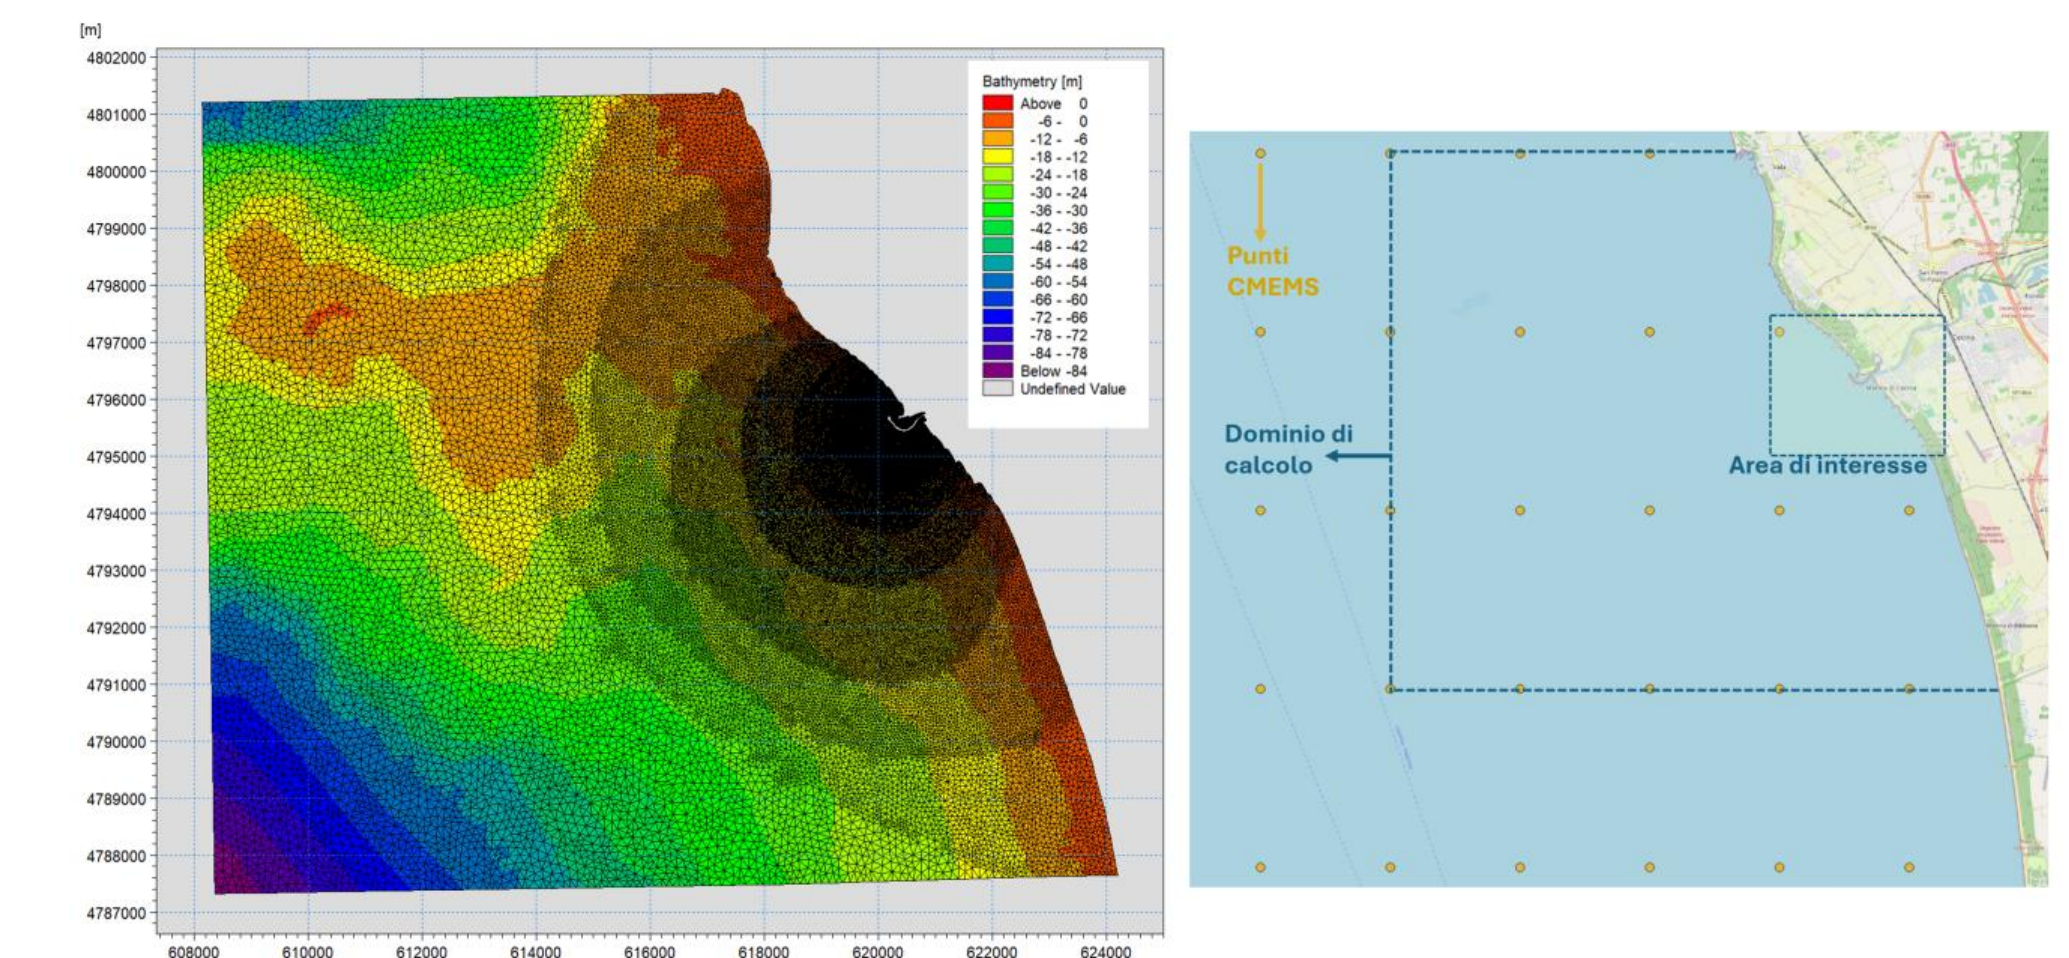
\includegraphics[width=\linewidth]{dominio_batimetria.png}
  \caption{Dominio di calcolo del modello idrodinamico. A sinistra: batimetria e mesh a
           elementi triangolari di dimensione variabile (pi\`u fitta nella zona di
           interesse). A destra: estensione del dominio ($\sim$$16\times14\,\text{km}$),
           area di interesse (riquadro) da cui \`e estratto il dataset e nodi CMEMS lungo i
           bordi usati per le condizioni al contorno. Baia di Cecina (costa toscana).}
  \label{fig:dominio}
\end{figure}

\subsection{Forzanti e condizioni al contorno}
\label{sec:forzanti}

Il modello locale realizza un \emph{downscaling idrodinamico} del bacino del
Mediterraneo, incrementando la risoluzione spaziale da circa $4{,}5\,\text{km}$ del
modello a grande scala fino a circa $10\,\text{m}$ nell'area di interesse. Le condizioni
al contorno di livello della superficie libera e di velocit\`a della corrente sono
derivate dal prodotto CMEMS~\citep{cmems}
\texttt{MEDSEA\_\allowbreak ANALYSIS\_\allowbreak FORECAST\_\allowbreak PHY\_\allowbreak 006\_013},
che fornisce dati orari delle componenti zonale e meridionale della velocit\`a di
corrente e del livello marino. Per ciascun nodo di calcolo ai bordi del dominio sono
imposte condizioni al contorno di tipo \emph{Flather}~\citep{oddo_pinardi}, mediante
l'imposizione dei valori orari delle componenti $(u, v)$ e dell'elevazione della
superficie libera, interpolati linearmente dai nodi CMEMS disponibili lungo i bordi.

La forzante di vento \`e imposta come variabile nel tempo e costante sul dominio, ed \`e
estratta dal dataset di \emph{reanalysis} \textbf{ERA5}~\citep{era5} dell'ECMWF
(componenti del vento a $10\,\text{m}$, $u_{10}, v_{10}$, a risoluzione oraria). In questa
fase non vengono considerati alcuni contributi al trasporto assunti come secondari: le
correnti indotte dal moto ondoso (deriva litoranea, correnti di ritorno) e gli apporti di
acqua dolce (scarichi fluviali, runoff superficiale).

\subsection{Scenari idrodinamici e di vento}
\label{sec:scenari}

Le serie temporali CMEMS ai bordi del dominio (2024--2025) sono state classificate in
finestre di 48 ore tramite descrittori sintetici (intensit\`a media della corrente,
persistenza direzionale, variabilit\`a del livello marino) e raggruppate con un algoritmo
di \emph{clustering} k-means in 4 classi idrodinamiche di riferimento, che rappresentano
regimi distinti in termini di intensit\`a della corrente, persistenza direzionale e
variabilit\`a del livello: dalla Classe~1 (regime moderato con elevata variabilit\`a del
livello) alla Classe~4 (regime energetico e altamente persistente). Le simulazioni
adottate in questa fase si riferiscono alla sola \textbf{Classe 2} (regime moderato e
persistente, con correnti di intensit\`a intermedia, direzione stabile e bassa
variabilit\`a del livello, ovvero condizioni relativamente stazionarie e ben organizzate),
rappresentata dalla finestra del 19--20 maggio 2024.

Analogamente, l'analisi statistica delle serie di vento ERA5 (intensit\`a, direzione,
persistenza; Figura~\ref{fig:rosa_venti}) ha portato a definire \textbf{4 classi di vento}
rappresentative, sovrapposte alla condizione idrodinamica di riferimento:
\begin{itemize}
    \item \textbf{V0} --- \emph{condizioni di calma / vento debole}. Vento di bassa
          intensit\`a (circa 1{,}5--2\,m/s), senza una direzione dominante significativa;
          rappresenta condizioni con forcing eolico trascurabile.
    \item \textbf{V1} --- \emph{vento persistente da NO}. Direzione prevalente compresa tra
          310\textdegree{} e 330\textdegree, con velocit\`a
          fino a 8--10\,m/s; rappresenta uno dei regimi dominanti lungo costa.
    \item \textbf{V2} --- \emph{vento persistente da SO}. Direzione prevalente tra
          230\textdegree{} e 250\textdegree, con velocit\`a
          fino a 8--10\,m/s; rappresenta il regime opposto rispetto al precedente, con
          effetti rilevanti sull'inversione del trasporto lungo costa.
    \item \textbf{V3} --- \emph{vento da settore orientale}. Direzione prevalente tra
          110\textdegree{} e 130\textdegree, con velocit\`a
          fino a 6--8\,m/s; rappresenta un regime meno frequente ma significativo, associato
          a condizioni di trasporto trasversale o secondario.
\end{itemize}

\begin{figure}[H]
  \centering
  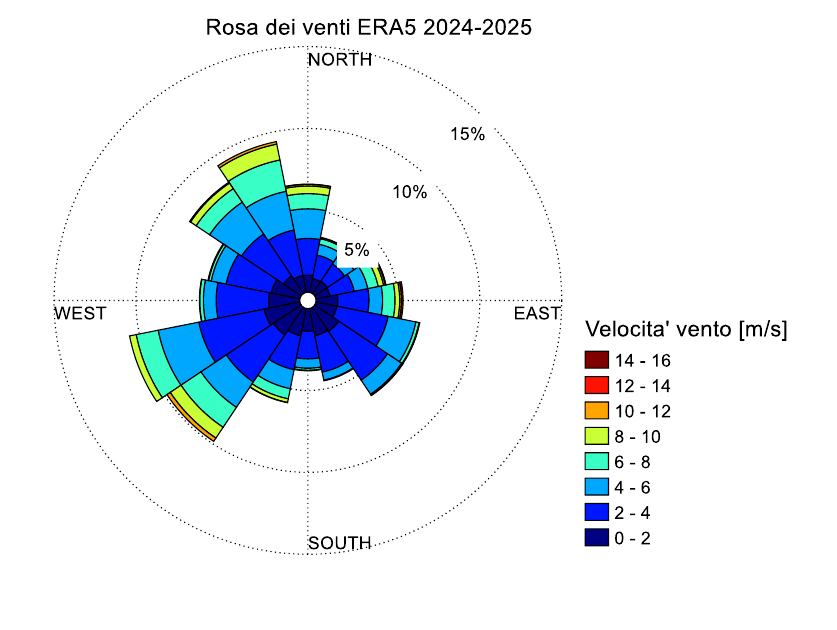
\includegraphics[width=0.62\linewidth]{rosa_venti.png}
  \caption{Rosa dei venti dell'area (dati ERA5 2024--2025): distribuzione di frequenza per
           direzione e intensit\`a. I settori dominanti da NO e da SO --- ben visibili ---
           motivano le classi di vento V1 e V2; le classi V0--V3 sintetizzano in modo
           compatto questa climatologia eolica.}
  \label{fig:rosa_venti}
\end{figure}

Per le classi V1--V3 il vento \`e modellato con un profilo temporale tipico: 8 ore di
calma iniziale, 6 ore di aumento lineare fino all'intensit\`a massima, 12 ore di intensit\`a
massima e 6 ore di diminuzione lineare. Ogni scenario genera plume con morfologie
marcatamente diverse (Figura~\ref{fig:plume}): da configurazioni compatte e direzionate a
configurazioni diffuse e frammentate.

\begin{figure}[H]
  \centering
  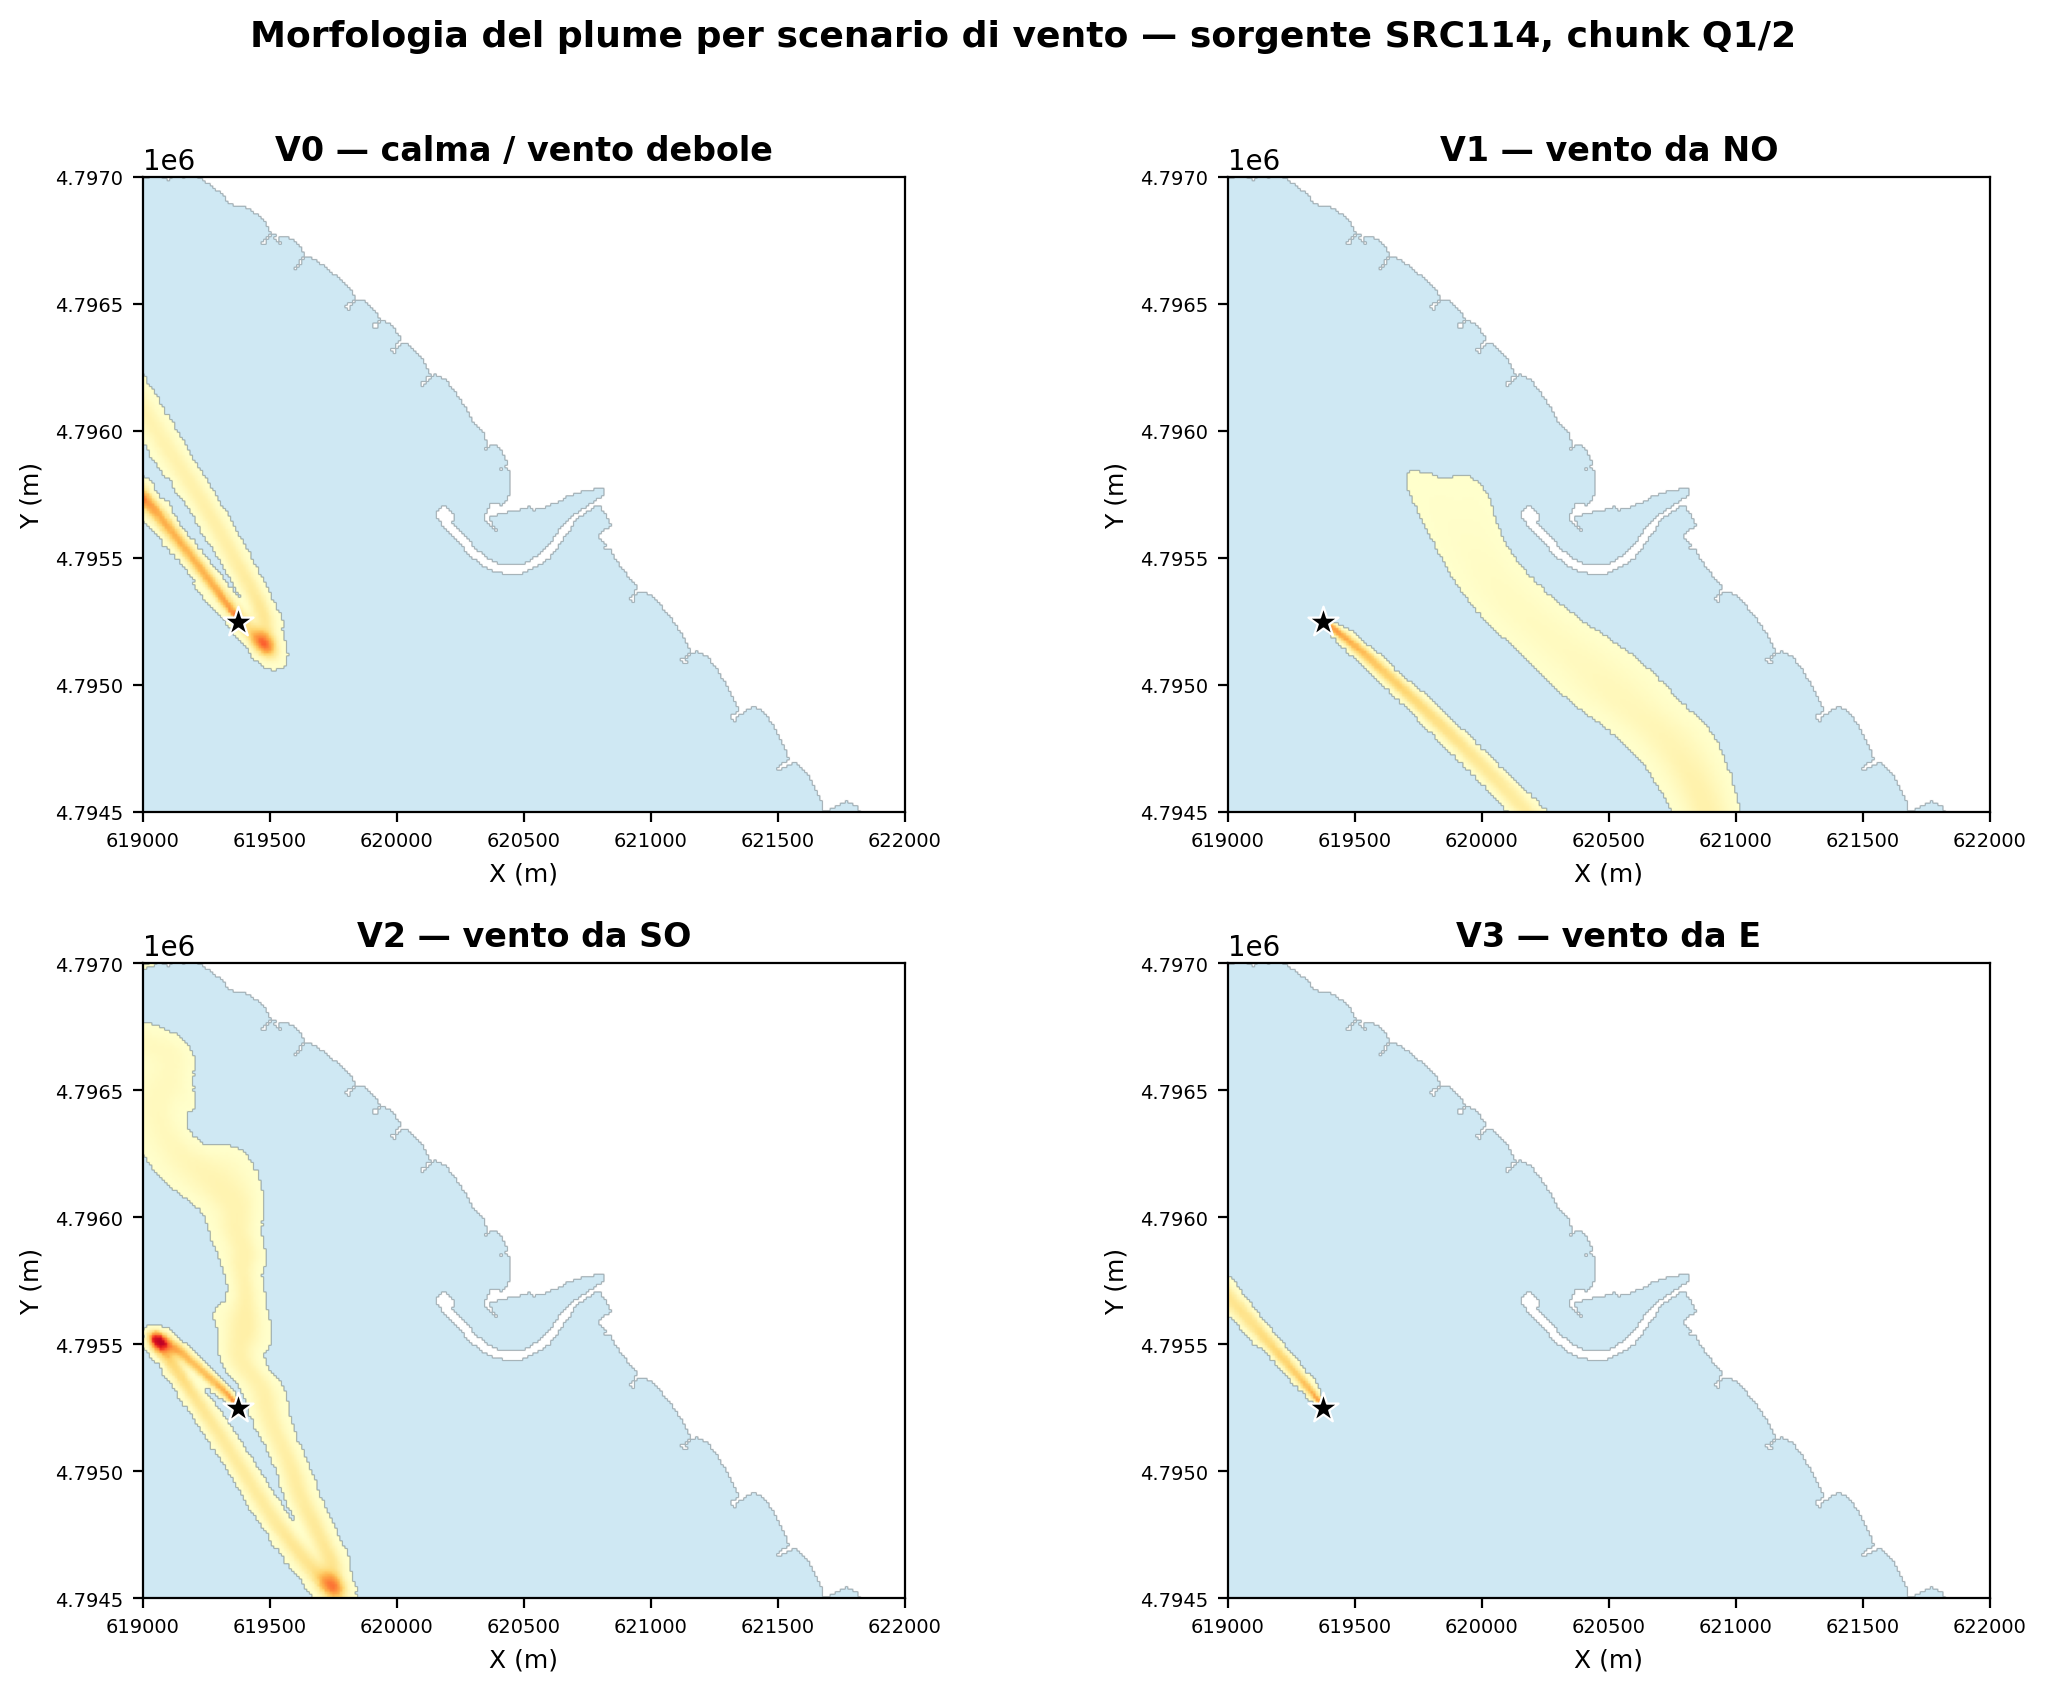
\includegraphics[width=\linewidth]{plume_scenarios.png}
  \caption{Campo di concentrazione del contaminante (plume) per la stessa sorgente
           ($\star$) sotto i quattro scenari di vento, allo stesso istante (chunk Q1/2).
           In V0 (calma) il plume resta compatto attorno alla sorgente; con vento
           persistente (V1 da NO, V2 da SO) viene avvettato lungo costa e si allunga/diffonde;
           in V3 (da E) \`e sospinto verso il largo. Mare in azzurro, terraferma in bianco,
           concentrazione in scala gialla--rossa.}
  \label{fig:plume}
\end{figure}

\subsection{Sorgenti e formato dei dati}
\label{sec:sorgenti}

Nell'area di interesse sono distribuite \textbf{132 sorgenti} equispaziate di circa
$200\,\text{m}$, ciascuna caratterizzata da una portata costante di $50\,\text{l/s}$ e da
una concentrazione di $1000\,\text{g/m}^3$ dell'inquinante target. Ogni sorgente \`e
simulata sotto i 4 scenari di vento, per un totale di $132 \times 4 = 528$ simulazioni.
I campi di concentrazione risultanti sono estratti in formato \textbf{NetCDF} su una
griglia regolare con passo di $10\,\text{m}$ e intervallo temporale di 2 minuti,
nell'area compresa fra le coordinate $x \in [619000, 622000]$ e
$y \in [4794500, 4797000]$\,m (UTM32N), corrispondente a un riquadro di
$3 \times 2{,}5\,\text{km}$ ($300 \times 250$ celle). I file seguono la convenzione di
nome \texttt{CL02\_<vento>\_SRC<num>\_Conc\_10mGrid.nc}; i corrispondenti campi di
corrente $(u, v)$, comuni a tutte le sorgenti di uno stesso scenario, seguono la
convenzione \texttt{CL02\_<vento>\_U\_V\_10mGrid.nc} (i campi di corrente sono comuni a
tutte le sorgenti di uno stesso scenario, in quanto la presenza della sorgente altera il
campo di moto solo localmente). Sorgente e scenario di ciascun file sono ricavati dal nome
tramite una semplice espressione regolare:

\begin{lstlisting}
m = re.match(r"CL02_(V\d)_(SRC\d+)_Conc", filename)
version, source_id = m.group(1), m.group(2)   # es. ("V2", "SRC042")
\end{lstlisting}

\subsection{Suddivisione del dataset e augmentation temporale}
\label{sec:split}

La suddivisione del dataset e l'augmentation temporale descritte di seguito sono
\textbf{comuni a entrambi gli approcci} confrontati nella tesi (Capitoli~\ref{cap:fcm}
e~\ref{cap:rl}), e fanno quindi parte dell'impostazione condivisa dell'ambiente di
simulazione.

Per garantire una valutazione su sorgenti mai osservate durante l'addestramento del
modello RL, le 132 sorgenti sono suddivise in un insieme di \textbf{training}
(SRC001--SRC106, 80\%, 106 sorgenti) e in un insieme di \textbf{inferenza} held-out
(SRC107--SRC132, 20\%, 26 sorgenti), riservato alla sola valutazione. Le stesse 26
sorgenti held-out sono usate per valutare sia il metodo del gradiente sia il modello RL,
cos\`i da garantire un confronto equo tra i due approcci.

Poich\'e il campo evolve nel tempo, ogni simulazione viene inoltre suddivisa in
\textbf{3 chunk temporali} che corrispondono a diversi stadi della dispersione del plume
e fungono da condizioni iniziali distinte: \textbf{Q1/4} (inizio della propagazione,
plume compatto), \textbf{Q1/2} (stadio intermedio, plume parzialmente disperso) e
\textbf{Q3/4} (stadio avanzato, plume pesantemente disperso). Questa
\emph{augmentation temporale} consente di inizializzare l'agente in tre fasi diverse della
dispersione, aumentando la variabilit\`a delle condizioni. La combinazione di scenari di
vento e chunk temporali definisce le \emph{configurazioni} $(v, q)$ su cui sono
articolati i risultati nei capitoli seguenti. In codice, la suddivisione delle sorgenti e
la mappatura chunk\,$\to$\,frame iniziale si riducono a:

\begin{lstlisting}
sources = sorted(discover_sources())               # SRC001 ... SRC132
train = [s for s in sources if int(s[3:]) <= 106]  # 80%
test  = [s for s in sources if int(s[3:]) >  106]  # 20% held-out

nt = field.n_timesteps                             # numero di frame
spawn_frame = {0: nt//4, 1: nt//2, 2: (nt*3)//4}[chunk_id]   # Q1/4, Q1/2, Q3/4
\end{lstlisting}

\section{Caricamento e gestione dei dati}
\label{sec:dataloader}

Il caricamento dei dati grezzi e la loro trasformazione in strutture interrogabili
dall'ambiente sono gestiti dal modulo software \texttt{data\_loader}, organizzato attorno
a tre componenti principali.

\paragraph{Campo di concentrazione.}
Il componente \texttt{NetCDFLoader} legge un file NetCDF e ne costruisce un oggetto
\texttt{ConcentrationField}, che incapsula i dati di concentrazione $[t, y, x]$ e
fornisce query spazio-temporali continue. Data una posizione $(x, y)$ e un istante $t$,
il campo restituisce la concentrazione tramite interpolazione (bilineare nello spazio,
lineare tra i due frame temporali adiacenti), cos\`i che l'agente non sia vincolato ai
soli centri-cella della griglia. All'inizializzazione, dalla maschera di terra viene
inoltre precalcolata --- tramite \emph{Euclidean Distance Transform} (EDT) --- una mappa
delle distanze dalla costa, usata sia per i vincoli di spawn sia per la penalit\`a di
prossimit\`a alla terra. In pratica, caricamento e interrogazione del campo si riducono a:

\begin{lstlisting}
field = NetCDFLoader(data_dir).load("CL02_V2_SRC042_Conc_10mGrid.nc")
field.set_time(t_idx)                 # seleziona il frame temporale corrente
c = field.get_concentration(x, y)     # concentrazione interpolata nel punto (x, y)
\end{lstlisting}

\paragraph{Campi di vento e corrente.}
In modo analogo, \texttt{WindData} e \texttt{CurrentData} incapsulano rispettivamente la
serie temporale di vento e il campo vettoriale di corrente, esponendo le componenti
$(u, v)$ in funzione del tempo (e della posizione, per la corrente). La sincronizzazione
temporale con il campo di concentrazione \`e mantenuta in minuti simulati.

\paragraph{Gestione centralizzata.}
Il componente \texttt{DataManager} coordina l'accesso ai dati: alla creazione
\emph{scopre automaticamente} le sorgenti disponibili dai file presenti, e su richiesta
fornisce all'ambiente il campo di concentrazione di una data coppia (sorgente, scenario)
insieme ai relativi vento e corrente. Per evitare di diventare un collo di bottiglia di
I/O durante l'addestramento --- che richiede milioni di passi e quindi continue
riletture --- il \texttt{DataManager} mantiene in memoria una \emph{cache} dei quattro
scenari di vento e corrente, eliminando gli accessi al disco dopo il primo caricamento.
Una singola chiamata restituisce il campo di concentrazione e le forzanti coerenti:

\begin{lstlisting}
# Campo di una coppia (sorgente, scenario) + forzanti della STESSA versione
field, run_id = data_manager.get_random_field_for_source_version("SRC042", "V2")
wind    = data_manager.get_wind_data_for_run(run_id, wind_mapping)       # da cache
current = data_manager.get_current_data_for_run(run_id, current_mapping) # da cache
\end{lstlisting}

\subsection{Sincronizzazione dei dati}
\label{sec:sync}

Affinch\'e l'agente percepisca un ambiente fisicamente coerente, i tre flussi di dati
--- concentrazione, vento e corrente --- devono essere allineati. Il \texttt{DataManager}
garantisce due livelli di sincronizzazione.

\paragraph{Sincronizzazione di versione.}
La versione dello scenario di vento (V0--V3) \`e codificata nel nome di ogni file (es.\
\texttt{CL02\_V2\_SRC042\_Conc\_10mGrid.nc}). Al momento di fornire un campo, il
\texttt{DataManager} estrae la versione dal nome del file di concentrazione e seleziona i
corrispondenti campi di vento e corrente della \emph{stessa} versione. In questo modo \`e
impossibile un accoppiamento errato tra concentrazione e forzanti: il plume \`e sempre
associato al vento e alla corrente che lo hanno effettivamente generato.

\paragraph{Sincronizzazione temporale.}
I tre flussi hanno cadenze di campionamento native diverse: il campo di concentrazione
MIKE21 \`e prodotto con un \emph{frame} ogni $\Delta t_c = 2\,\text{min}$, mentre vento e
corrente seguono le rispettive serie, ciascuna con il proprio passo ($\Delta t_w$ per il
vento, $\Delta t_u$ per la corrente). Se questi flussi non fossero allineati, l'agente
percepirebbe un plume che avanza a una velocit\`a incoerente con il vento e la corrente che
lo trasportano. L'ambiente li riconduce perci\`o a un unico \textbf{asse temporale
assoluto}, espresso in \emph{minuti simulati}.

\medskip\noindent\emph{Istante assoluto.} Ad ogni passo, dallo step corrente si ricava
l'istante assoluto dell'episodio come somma dell'offset del chunk di partenza e del tempo
trascorso:
\begin{equation}
  t_{\text{abs}}(k) = \underbrace{f_0 \cdot \Delta t_c}_{\text{offset del chunk}}
  \;+\; \underbrace{k \cdot \Delta t / 60}_{\text{tempo trascorso}}
  \qquad [\text{min}],
  \label{eq:tabs}
\end{equation}
dove $k$ \`e il numero di step compiuti, $\Delta t = 10\,\text{s}$ il passo dell'agente e
$f_0$ il \emph{frame} di spawn del chunk (Sezione~\ref{sec:split}). \`E essenziale che
l'offset del chunk compaia in $t_{\text{abs}}$: cos\`i, quando l'episodio parte da Q3/4, non
solo il plume ma anche il vento e la corrente sono presi al punto \emph{corrispondente} del
loro profilo temporale --- l'agente incontra lo stato idrodinamico effettivamente
contemporaneo a quello stadio di dispersione, non quello dell'inizio simulazione.

\medskip\noindent\emph{Query per flusso e interpolazione.} L'istante $t_{\text{abs}}$ viene
poi convertito nell'indice, in generale \emph{frazionario}, proprio di ciascun flusso; il
valore restituito \`e l'\textbf{interpolazione lineare} tra i due campioni adiacenti:
\begin{itemize}[leftmargin=1.4em, itemsep=2pt]
  \item \textbf{concentrazione}: l'indice di frame \`e
        $f = f_0 + (t_{\text{abs}} - f_0\,\Delta t_c)/\Delta t_c$; detta $\alpha$ la sua parte
        frazionaria, il campo restituito \`e la miscela
        $(1-\alpha)\,C_{t_0} + \alpha\,C_{t_1}$ tra i frame adiacenti $t_0=\lfloor f\rfloor$ e
        $t_1=t_0+1$ --- interpolazione temporale che si somma a quella bilineare nello spazio
        (Sezione~\ref{sec:dataloader});
  \item \textbf{vento e corrente}: l'indice \`e $t_{\text{abs}}/\Delta t_{w,u}$, con analoga
        miscela lineare tra i campioni delle rispettive serie.
\end{itemize}

\medskip\noindent\emph{Cadenza.} Poich\'e
$\Delta t_c / \Delta t = 2\,\text{min} / 10\,\text{s} = 12$, il campo di concentrazione
avanza di un frame \textbf{ogni 12 step} dell'agente; nei passi intermedi l'agente non vede
un fotogramma ``congelato'' ma una versione \emph{interpolata} del campo. Ad esempio, dopo
$11$ minuti dallo spawn ($k = 66$) l'indice di frame vale $f_0 + 5{,}5$: il campo restituito
\`e la media al $50\%$ fra il frame $f_0{+}5$ e il frame $f_0{+}6$
(Figura~\ref{fig:timeline}).

\begin{figure}[H]
\centering
\begin{tikzpicture}[font=\footnotesize, x=2.7cm]
  \draw[-{Latex[length=2mm]}] (-0.15,0) -- (4.55,0) node[right]{$t$ [min]};
  % frame di concentrazione (tick alti)
  \foreach \x/\lab in {0/$f_0$, 2/$f_0{+}5$, 4/$f_0{+}6$}{
    \draw[thick] (\x,-0.12) -- (\x,0.36);
    \node[above, font=\scriptsize] at (\x,0.34) {\lab};
  }
  \node[below, font=\scriptsize] at (2,-0.12){$10$}; \node[below, font=\scriptsize] at (4,-0.12){$12$};
  % step dell'agente (tick corti tra frame f0+5 e f0+6)
  \foreach \i in {1,...,11}{ \draw[gray] ({2+\i/6},-0.06) -- ({2+\i/6},0.06); }
  % query a t=11 min (indice f0+5.5)
  \draw[densely dashed, red!70!black] (3,-0.16) -- (3,0.62);
  \node[red!70!black, above, font=\scriptsize, align=center] at (3,0.6){$k{=}66$\\($11$\,min)};
  \draw[{Latex[length=1.5mm]}-{Latex[length=1.5mm]}, blue!55!black] (2,0.18) -- (3,0.18)
       node[midway, above, font=\scriptsize]{$\alpha$};
  \draw[{Latex[length=1.5mm]}-{Latex[length=1.5mm]}, blue!55!black] (3,0.18) -- (4,0.18)
       node[midway, above, font=\scriptsize]{$1-\alpha$};
  \node[align=center, font=\scriptsize, gray!50!black] at (3,-0.62)
       {$12$ step dell'agente ($\Delta t{=}10$\,s) per ogni frame ($\Delta t_c{=}2$\,min)};
\end{tikzpicture}
\caption{Sincronizzazione temporale della concentrazione. Tra due frame consecutivi
         ($f_0{+}5$ a $10\,\text{min}$, $f_0{+}6$ a $12\,\text{min}$) l'agente compie 12 step;
         allo step $k{=}66$ ($11\,\text{min}$) il campo \`e la miscela lineare
         $(1-\alpha)C_{f_0+5} + \alpha C_{f_0+6}$ con $\alpha = 0{,}5$. Vento e corrente sono
         interpolati in modo analogo sulle rispettive serie.}
\label{fig:timeline}
\end{figure}

\medskip\noindent\emph{Gestione dei bordi.} Un episodio dura al pi\`u $1080$ step
($= 180\,\text{min}$); partendo da un chunk avanzato, $t_{\text{abs}}$ pu\`o oltrepassare la
fine di una serie. In tal caso l'indice viene \textbf{saturato} all'ultimo campione
disponibile (con un avviso una tantum per il vento), cos\`i che l'episodio resti sempre ben
definito anche quando ``sopravvive'' ai dati. In codice, l'aggiornamento dei tre flussi ad
ogni step si riduce a:

\begin{lstlisting}
dt_c  = 2.0                                       # min per frame di concentrazione
t_abs = f0 * dt_c + step * dt / 60.0              # istante assoluto in minuti simulati
field.set_time(f0 + (step * dt / 60.0) / dt_c)    # frame float -> interp. temporale lineare
wind.set_time_from_minutes(t_abs)                 # indice = t_abs / dt_wind  (clamp agli estremi)
current.set_time_from_minutes(t_abs)              # indice = t_abs / dt_curr  (clamp agli estremi)
\end{lstlisting}
            % Cap. 2 --- Il dataset
\chapter{Composizione dell'ambiente}
\label{cap:ambiente}

A partire dai dati descritti nel Capitolo~\ref{cap:dati}, questo capitolo illustra
l'\textbf{ambiente di simulazione} vero e proprio: l'interfaccia software che trasforma i
campi idrodinamici in un problema di controllo sequenziale, la struttura della squadra di
agenti, lo spazio delle azioni, i vincoli di navigazione, la procedura di inizializzazione
e il segnale di reward. Si tratta dell'infrastruttura \textbf{condivisa} dai due approcci
confrontati nella tesi: sia il metodo del gradiente (Capitolo~\ref{cap:fcm}) sia l'agente
PPO (Capitolo~\ref{cap:rl}) operano su questo stesso ambiente, con la stessa dinamica e
gli stessi vincoli. L'unica differenza risiede nel modulo che, ricevuta l'osservazione,
sceglie l'azione: una regola analitica nel primo caso, una rete neurale addestrata nel
secondo.

\section{L'ambiente software}
\label{sec:env}

L'ambiente \`e implementato dalla classe \texttt{SourceSeekingEnv} secondo l'interfaccia
standard \texttt{gymnasium.Env}. Esso riceve in ingresso un \texttt{ConcentrationField}
(con i relativi \texttt{WindData} e \texttt{CurrentData}), oppure un \texttt{DataManager}
da cui estrarre dinamicamente un campo casuale ad ogni episodio --- modalit\`a usata in
addestramento per variare di continuo sorgente e scenario. Il dominio \`e la griglia
regolare $300 \times 250$ celle a passo $10\,\text{m}$ ($3 \times 2{,}5\,\text{km}$)
descritta nella Sezione~\ref{sec:sorgenti}.

L'oggetto ambiente viene quindi incapsulato in una catena di \emph{wrapper}:
\begin{itemize}
    \item un \texttt{ActionMasker} che applica l'action masking
          (Sezione~\ref{sec:masking}), escludendo le azioni non ammissibili;
    \item un \emph{vettorizzatore} (\texttt{DummyVecEnv}) che uniforma l'interfaccia a
          quella attesa dalla libreria di RL;
    \item per il solo addestramento RL, un \texttt{VecNormalize} che normalizza le
          osservazioni con media e varianza stimate online.
\end{itemize}

\begin{lstlisting}
raw = SourceSeekingEnv(config, concentration_field=field,
                       wind_data=wind, current_data=current)
env = ActionMasker(raw, mask_fn)               # masking delle azioni
env = DummyVecEnv([lambda: env])               # vettorizzazione
env = VecNormalize(env, norm_reward=False)     # solo per il training RL
\end{lstlisting}

\subsection{Architettura master--slave}
\label{sec:master_slave}

Il sistema \`e organizzato come una \textbf{squadra di agenti} in formazione
\emph{master--slave}. L'agente \textbf{master} \`e l'unico a decidere il movimento e a
spostarsi attivamente sul dominio; attorno ad esso, otto agenti \textbf{slave}
mantengono una formazione rigida (Figura~\ref{fig:formazione}), posizionandosi a distanza
$r_s$ (il \emph{sensor range}) lungo le otto direzioni cardinali e diagonali $\hat{d}_i$ (N, S, E, O, NE, SE,
NO, SO). Ciascuno slave campiona la concentrazione del contaminante nella propria
posizione $\mathbf{p} + r_s\,\hat{d}_i$ e la riporta al master, senza alcuna autonomia
decisionale propria: il loro unico compito \`e fornire le misurazioni e conservare la
formazione rispetto al master mentre questo si muove.

Le otto misurazioni degli slave, insieme alla lettura del master nella posizione
centrale, costituiscono l'informazione locale sul campo di concentrazione su cui si
basano entrambi gli approcci. Nel metodo del gradiente tali letture vengono usate per
stimare il gradiente locale; nell'approccio RL confluiscono nello spazio di osservazione
della rete neurale che governa il master. Le posizioni degli slave e il relativo
campionamento si esprimono come:

\begin{lstlisting}
DIAG = 1 / np.sqrt(2)
DIRECTIONS = np.array([(0,1),(0,-1),(1,0),(-1,0),          # N, S, E, O
                       (DIAG,DIAG),(DIAG,-DIAG),
                       (-DIAG,DIAG),(-DIAG,-DIAG)])         # diagonali
# ogni slave campiona a distanza r_s lungo la propria direzione
readings = [field.get_concentration(*(master_pos + r_s * d)) for d in DIRECTIONS]
\end{lstlisting}

\begin{figure}[H]
\centering
\begin{tikzpicture}[
  font=\footnotesize,
  slave/.style={circle, draw, fill=blue!14, minimum size=6.5mm, inner sep=0pt},
  master/.style={circle, draw, fill=orange!75, minimum size=9mm, inner sep=0pt},
  link/.style={-, gray, densely dashed}
]
  \def\R{2.3}
  \draw[gray!45, densely dotted] (0,0) circle (\R);
  \foreach \a/\lab in {90/N, 270/S, 0/E, 180/O, 45/NE, 315/SE, 135/NO, 225/SO} {
    \draw[link] (0,0) -- (\a:\R);
    \node[slave] at (\a:\R) {\scriptsize S};
    \node[gray!60!black] at (\a:{\R+0.42}) {\lab};
  }
  \node[master] (m) at (0,0) {\scriptsize M};
  \draw[{Latex}-{Latex}, thick] (0,0) -- (20:\R)
       node[midway, above, sloped, fill=white, inner sep=1pt]{$r_s$};
\end{tikzpicture}
\caption{Formazione master--slave. L'agente \textbf{master} (M, arancio) occupa il centro;
         otto agenti \textbf{slave} (S, blu) sono disposti a distanza $r_s$ (il \emph{sensor
         range}) lungo le direzioni cardinali e diagonali. Ogni slave campiona la
         concentrazione nella propria posizione e la riporta al master; le stesse otto
         direzioni sono anche le azioni di movimento disponibili.}
\label{fig:formazione}
\end{figure}

Questa unica corona di 8 sensori \`e la configurazione base (\emph{singola corona}); il
Capitolo~\ref{cap:rl} valuta anche una variante a \textbf{doppia corona} che aggiunge una
seconda formazione di 8 slave a $r_{s2} = 50\,\text{m}$, per dare al master informazione
sul plume a scala spaziale pi\`u larga.

\subsection{Spazio delle azioni e dinamica dell'episodio}
\label{sec:dinamica}

Il master si muove con uno spazio delle azioni discreto a \textbf{8 direzioni}
(le stesse $\hat{d}_i$ della formazione), con velocit\`a nominale di $1\,\text{m/s}$ e
passo temporale $\Delta t = 10\,\text{s}$, spostandosi quindi di $10\,\text{m}$ per
azione (o $\sim$7\,m per componente nelle direzioni diagonali). Ogni episodio ha durata
massima di 1080 step ($= 3\,\text{h}$ di tempo simulato) e termina con \textbf{successo}
quando il master raggiunge la sorgente (distanza $\leq 50\,\text{m}$). Il campo di
concentrazione evolve durante l'episodio: ogni alcuni step dell'agente il campo MIKE21
avanza di un frame temporale, mantenendo vento e correnti sincronizzati. La conversione
azione\,$\to$\,spostamento \`e immediata:

\begin{lstlisting}
ACTION_MAP = {0:(0,1), 1:(0,-1), 2:(1,0), 3:(-1,0),       # N, S, E, O
              4:(DIAG,DIAG), 5:(DIAG,-DIAG),
              6:(-DIAG,DIAG), 7:(-DIAG,-DIAG)}            # diagonali
dx, dy = ACTION_MAP[action]
step = max_velocity * dt                  # 1 m/s * 10 s = 10 m
master_pos += np.array([dx, dy]) * step
\end{lstlisting}

Questo spazio d'azione a passo fisso \`e il punto di partenza; il Capitolo~\ref{cap:rl} lo
estende a \textbf{velocit\`a variabile} rendendo la velocit\`a stessa una scelta
dell'agente (spazio $\text{Discrete}(8\times K)$), cos\`i che il master decida a ogni passo
non solo la direzione ma anche l'entit\`a dello spostamento.

\subsection{Action masking}
\label{sec:masking}

Per impedire le collisioni con la costa, l'ambiente calcola ad ogni passo una
\emph{maschera} delle azioni: le direzioni che porterebbero il master sulla terraferma o
fuori dal dominio vengono escluse dall'insieme delle azioni ammissibili. Questo
meccanismo, sfruttato sia dal metodo del gradiente sia dall'agente RL, garantisce che
vengano percorse soltanto traiettorie valide senza dover penalizzare a posteriori le
azioni non consentite.

\begin{lstlisting}
def action_masks(self):
    masks = np.ones(8, dtype=bool)
    step = self.max_velocity * self.dt
    for a, (dx, dy) in ACTION_MAP.items():
        nx, ny = self.x + dx*step, self.y + dy*step
        if out_of_domain(nx, ny) or self.field.is_land(nx, ny):
            masks[a] = False                  # azione invalida
    return masks
\end{lstlisting}

La maschera \`e costruita a partire dalla \emph{land mask} del campo e dalla mappa delle
distanze dalla costa precalcolata via \emph{Euclidean Distance Transform} (EDT,
Sezione~\ref{sec:dataloader}): la stessa mappa fornisce anche la penalit\`a di prossimit\`a
alla terra usata nel segnale di reward (Sezione~\ref{sec:reward}).

\subsection{Inizializzazione dell'agente}
\label{sec:spawn}

Il master viene inizializzato su una cella appartenente al plume (concentrazione
$c \geq 0{,}5$), a distanza dalla costa $\geq 50\,\text{m}$ e a una distanza dalla
sorgente controllata. Nel corso del progetto si sono succeduti \textbf{due algoritmi di
spawn}, e quale dei due sia in uso dipende dalla fase di lavoro: gli addestramenti iniziali
(a velocit\`a fissa) adottano una \emph{cascata di anelli} a soglie fisse, mentre a partire
dall'analisi a velocit\`a variabile (Sezione~\ref{sec:rl_velocity}) si passa a un
\emph{disco adattivo} $[d_{\min},d_{\max}]$ con campionamento uniforme in distanza. Vanno
descritti entrambi perch\'e coesistono nei risultati riportati: ogni modello eredita
l'algoritmo in vigore quando \`e stato addestrato, e i confronti fra modelli tengono conto
di questa differenza.

\paragraph{Primo algoritmo (addestramenti a velocit\`a fissa): cascata di anelli.}
La procedura iniziale (Figura~\ref{fig:spawn_cascade}) scandisce una lista di anelli in
ordine decrescente di distanza dalla sorgente, restituendo una cella a caso del
\emph{primo anello non vuoto}:
\begin{center}
$(2000\text{--}2500) \to (1500\text{--}2000) \to (1000\text{--}1500) \to
(500\text{--}1000) \to (250\text{--}500) \to (50\text{--}250) \to (0\text{--}50)\;\text{m}$
\end{center}
Per ogni anello vengono selezionate le celle con $c \geq 0{,}5$ e distanza dalla terra
$\geq 50\,\text{m}$; la cascata scende all'anello successivo solo se nessuna cella del
corrente soddisfa entrambe le condizioni. La distanza iniziale media di spawn risulta di
circa $800\,\text{m}$.

\begin{lstlisting}
CASCADE = [(2000,2500),(1500,2000),(1000,1500),
           (500,1000),(250,500),(50,250),(0,50)]
for dmin, dmax in CASCADE:                    # dal piu' lontano al piu' vicino
    cells = plume_cells[(dist >= dmin) & (dist <= dmax) & (land_dist >= 50)]
    if len(cells):
        return random.choice(cells)           # primo anello non vuoto
\end{lstlisting}

\begin{figure}[H]
\centering
\begin{tikzpicture}[font=\footnotesize]
  % anelli concentrici (1 unita' = 500 m); disegnati dal piu' grande al piu' piccolo
  \foreach \r/\col in {5/blue!22, 4/blue!18, 3/blue!14, 2/blue!11, 1/blue!8, 0.5/blue!5}{
    \fill[\col] (0,0) circle (\r);
  }
  \foreach \r in {0.1,0.5,1,2,3,4,5}{ \draw[gray!55] (0,0) circle (\r); }
  % sorgente
  \node[star, star points=5, fill=yellow, draw, minimum size=5mm, inner sep=0pt] at (0,0) {};
  % etichette distanze (m) sull'asse
  \foreach \r/\d in {0.5/250, 1/500, 2/1000, 3/1500, 4/2000, 5/2500}{
    \node[fill=white, inner sep=0.8pt, font=\scriptsize] at (\r,0) {\d};
  }
  % freccia: ordine di selezione dal piu' lontano al piu' vicino
  \draw[-{Latex[length=2.4mm]}, thick, orange!85!black] (4.6,0.55) to[bend right=12] (0.9,0.55);
  \node[orange!70!black, align=center, font=\scriptsize] at (2.7,1.35)
       {ordine di selezione\\(dal pi\`u lontano)};
\end{tikzpicture}
\caption{Cascata di anelli concentrici per l'inizializzazione. Il master \`e collocato in
         un anello attorno alla sorgente ($\star$), partendo dal pi\`u lontano
         ($2000$--$2500\,\text{m}$) e scendendo verso i pi\`u vicini solo se nessuna cella
         dell'anello corrente soddisfa i vincoli (concentrazione $\geq 0{,}5$, distanza dalla
         terra $\geq 50\,\text{m}$). Le distanze sono in metri dalla sorgente.}
\label{fig:spawn_cascade}
\end{figure}

\textbf{Pro.} Lo schema \`e semplice e deterministico nell'ordinamento, e privilegia in modo
naturale gli spawn lontani: con plume esteso l'agente parte quasi sempre dal bordo esterno,
affrontando il compito nella sua versione pi\`u difficile e informativa.
\textbf{Contro.} Restituendo sempre il \emph{primo} anello popolato, gli spawn si
\textbf{addensano quasi tutti alla stessa distanza} (l'anello esterno del plume del
momento): la distribuzione della distanza iniziale \`e di fatto degenere e copre male
l'intervallo intermedio. Le soglie sono inoltre \emph{fisse}, e non si adattano a plume
pi\`u compatti o pi\`u diffusi del previsto.

\paragraph{Secondo algoritmo (dall'analisi a velocit\`a variabile): disco adattivo $[d_{\min},\,d_{\max}]$.}
Per distribuire i punti di partenza su tutto l'intervallo utile, la versione definitiva
costruisce un \emph{disco di spawn} $[d_{\min},\,d_{\max}]$ che si adatta allo scenario e
campiona in modo \textbf{uniforme rispetto alla distanza} (Figura~\ref{fig:spawn_disk}).
Detto $\{d_i\}$ l'insieme delle distanze dalla sorgente delle celle di plume ammissibili
($c \geq 0{,}5$, distanza dalla terra $\geq 50\,\text{m}$):
\begin{itemize}
  \item $d_{\max} = \min\!\big(3000\,\text{m},\ \max_i d_i\big)$: il tetto di $3\,\text{km}$,
        abbassato all'estensione massima del plume quando questo non arriva cos\`i lontano;
  \item $d_{\min} = \max\!\big(300\,\text{m},\ \mathrm{perc}_{50}(\{d_i\})\big)$: la mediana
        delle distanze delle celle di plume, con un \emph{floor} assoluto a $300\,\text{m}$.
        Cos\`i $d_{\min}$ \textbf{scala con la diffusione del plume}: plume molto esteso
        $\Rightarrow$ celle lontane $\Rightarrow$ mediana alta $\Rightarrow$ $d_{\min}$ alta;
        plume compatto $\Rightarrow$ $d_{\min}$ bassa (una soglia alta sarebbe
        irraggiungibile). Il floor evita gli spawn gi\`a dentro il raggio di successo, tranne
        quando l'intero plume \`e pi\`u piccolo del floor stesso, nel qual caso il disco si
        restringe alla sua estensione;
  \item se $d_{\max}-d_{\min} < 500\,\text{m}$ si abbassa $d_{\min}$ (fino al floor) per
        garantire un intervallo abbastanza ampio da non far ripartire tutti gli agenti dalla
        stessa distanza.
\end{itemize}
Si estrae quindi una distanza obiettivo $d^\star \sim \mathcal{U}(d_{\min},\,d_{\max})$ e si
sceglie a caso una cella valida entro $\pm 50\,\text{m}$ da $d^\star$ (con piccolo jitter),
ripetendo finch\'e i vincoli di dominio, concentrazione e distanza dalla costa sono
soddisfatti. Campionando in modo uniforme $d^\star$, gli spawn si \textbf{spalmano su tutto}
$[d_{\min},\,d_{\max}]$ invece di concentrarsi sull'anello esterno.

\begin{lstlisting}
d = dist_from_source(plume_cells)          # celle con c>=0.5 e land>=50 m
d_disk = d[d <= 3000]                       # tetto d_cap = 3 km
d_max  = min(3000, d_disk.max())
d_min  = max(300, percentile(d_disk, 50))   # mediana, floor 300 m
if d_max - d_min < 500:                      # ampiezza minima dell'intervallo
    d_min = max(300, d_max - 500)
target = uniform(d_min, d_max)               # UNIFORME in distanza
band   = plume_cells[abs(d_disk - target) <= 50]   # cella entro +-50 m
return random.choice(band)                   # (con jitter +-5 m)
\end{lstlisting}

\begin{figure}[H]
\centering
\begin{tikzpicture}[font=\footnotesize]
  % 1 unita' = 500 m; disco esterno d_max, foro interno d_min
  \fill[blue!10] (0,0) circle (4.2);
  \fill[white]   (0,0) circle (1.5);
  \draw[dashed, thick, blue!55!black] (0,0) circle (1.5);
  \draw[dashed, thick, blue!55!black] (0,0) circle (4.2);
  % spawn estratti uniformemente in distanza nell'anello [d_min, d_max]
  \foreach \a/\r in {18/1.8, 52/3.5, 88/2.4, 124/3.9, 158/2.0, 196/3.2, 228/2.7,
                     262/4.0, 298/1.7, 332/3.0, 8/3.6, 72/2.9, 140/1.6, 210/2.3,
                     280/3.4, 350/2.6}{
    \fill[orange!85!black] (\a:\r) circle (1.6pt);
  }
  \node[star, star points=5, fill=yellow, draw, minimum size=5mm, inner sep=0pt] at (0,0) {};
  \draw[-{Latex[length=2mm]}, gray!65] (0,0) -- (68:1.5)
       node[pos=0.6, sloped, above, font=\scriptsize] {$d_{\min}$};
  \draw[-{Latex[length=2mm]}, gray!65] (0,0) -- (255:4.2)
       node[pos=0.72, sloped, below, font=\scriptsize] {$d_{\max}$};
\end{tikzpicture}
\caption{Disco di spawn adattivo $[d_{\min},d_{\max}]$ (versione adottata). $d_{\max}$ \`e il
         tetto di $3\,\text{km}$ ridotto all'estensione del plume; $d_{\min}$ \`e la mediana
         delle distanze delle celle di plume (\emph{floor} $300\,\text{m}$) e scala con la
         diffusione. I punti di partenza (arancioni) sono estratti in modo \emph{uniforme
         rispetto alla distanza} nell'anello, coprendo l'intero intervallo anzich\'e
         addensarsi sul bordo esterno.}
\label{fig:spawn_disk}
\end{figure}

\textbf{Pro.} Il disco \`e \emph{adattivo} (si ridimensiona con l'estensione del plume) e
distribuisce gli spawn in modo uniforme su tutto $[d_{\min},d_{\max}]$: la distanza iniziale
copre l'intero intervallo, rendendo il confronto fra modelli pi\`u equo e statisticamente
pi\`u solido. Il floor a $300\,\text{m}$ e l'ampiezza minima mantengono comunque il compito
non banale, senza inizializzazioni gi\`a prossime al bersaglio.
\textbf{Contro.} La logica \`e pi\`u complessa (percentile, banda di tolleranza, fallback),
e la distanza tipica di partenza non \`e un valore fisso ma dipende dalla mediana delle celle
di plume del singolo scenario, quindi varia da caso a caso. Soprattutto, campionando in modo
uniforme su $[d_{\min},d_{\max}]$, l'agente pu\`o partire anche da \textbf{distanze brevi}
(prossime a $d_{\min}$), mentre la cascata sceglieva sempre il punto valido pi\`u lontano:
alcuni episodi risultano quindi mediamente pi\`u facili rispetto al primo algoritmo.

\paragraph{Perch\'e il passaggio, e quale algoritmo usa cosa.}
Con la velocit\`a fissa la cascata era adeguata: il compito era gi\`a difficile e la distanza
di partenza, pur concentrata, risultava paragonabile fra episodi. Introducendo la
\textbf{velocit\`a variabile} (Sezione~\ref{sec:rl_velocity}) il confronto avviene per\`o
\emph{fra} modelli e \emph{fra} velocit\`a massime diverse: una distribuzione di spawn
degenere avrebbe reso i confronti sensibili al particolare anello estratto pi\`u che alla
reale capacit\`a dell'agente. Il disco adattivo, uniforme in distanza e indipendente dalla
forma istantanea del plume, offre una base di valutazione controllata e riproducibile. In
pratica: i modelli a \textbf{velocit\`a fissa} dei primi esperimenti usano la
\textbf{cascata}; tutti i modelli e le analisi a \textbf{velocit\`a variabile} --- l'intero
range di velocit\`a (Sezione~\ref{sec:rl_velocity}), i $v_{\max}$ intermedi, il confronto fra
corona singola e doppia e il test a singolo agente senza formazione --- usano il
\textbf{disco adattivo}.

L'analisi delle \emph{spawn map} (Sezione~\ref{sec:spawn_map}) verifica infine, per il disco,
che l'esito di un episodio non dipenda dalla particolare posizione di partenza.

\section{Il segnale di reward}
\label{sec:reward}

Oltre a osservazione e dinamica, l'ambiente calcola ad ogni passo un \textbf{segnale di
reward} scalare $r_t$. Esso \`e usato \emph{unicamente} dall'agente RL, che ne massimizza
il ritorno atteso in fase di addestramento (Capitolo~\ref{cap:rl}); il metodo del gradiente
lo ignora, poich\'e decide l'azione analiticamente dalle sole letture correnti. Nella sua
forma finale, adottata come riferimento, il reward combina un piccolo insieme di segnali
essenziali:
\begin{equation}
    r_t = \underbrace{r^{\text{reach}}_t}_{+100\ \text{a successo}}
        \;+\; \underbrace{r^{\text{dist}}_t}_{\text{avvicinamento}}
        \;+\; \underbrace{r^{\text{grad}}_t}_{\pm 0{,}05}
        \;+\; \underbrace{r^{\text{time}}_t}_{-0{,}1/\text{step}}
        \;+\; \underbrace{r^{\text{land}}_t}_{\text{costa}}
        \;+\; \underbrace{r^{\text{bound}}_t}_{-10\ \text{fuori dominio}}
    \label{eq:reward}
\end{equation}
dove: $r^{\text{reach}}_t = +100$ (pi\`u un piccolo bonus per l'arrivo anticipato) premia il
raggiungimento della sorgente; $r^{\text{dist}}_t$
\`e proporzionale alla \emph{riduzione} di distanza dalla sorgente nel passo (reward di
distanza lineare); $r^{\text{grad}}_t = \pm 0{,}05$ premia il muoversi lungo il gradiente
crescente di concentrazione; $r^{\text{time}}_t = -0{,}1$ per step incentiva a raggiungere
la sorgente rapidamente; $r^{\text{land}}_t$ penalizza la prossimit\`a eccessiva alla costa
(via la mappa EDT); $r^{\text{bound}}_t = -10$ penalizza l'uscita dal dominio. In codice, il
reward si assembla ad ogni passo come somma di questi contributi:

\begin{lstlisting}
def _compute_reward(self):
    r = 0.0
    if self._source_reached():                    # 1) raggiungimento (+ bonus di tempo)
        r += 100.0 + max(0, (N_max - k) / N_max * 50)
    if self._out_of_bounds():                     # 2) uscita dal dominio
        r += -10.0
    r += (prev_dist - curr_dist) * K_dist          # 3) distanza (lineare)
    r += 0.05 if conc > prev_conc else -0.05       # 4) gradiente di concentrazione
    r += -0.1                                       # 5) penalita' di tempo (per step)
    r += land_proximity_penalty(land_dist)         # 6) prossimita' alla costa (EDT)
    return r
\end{lstlisting}

La scelta di questa forma \emph{minimale} non \`e a priori: \`e il risultato di uno studio
di ablation (Sezione~\ref{sec:rl_reward}) che ha confrontato varianti pi\`u ricche ---
con reward di allineamento a vento e corrente, distanza quadratica, \emph{zone multiplier},
\emph{retreat asymmetry} e penalit\`a di stagnazione --- mostrando che i segnali aggiuntivi
non migliorano, e in alcuni casi peggiorano, le prestazioni. Il gradiente di concentrazione,
calcolato direttamente sul campo simulato, incorpora gi\`a implicitamente l'effetto di vento
e corrente.

        % Cap. 3 --- Composizione dell'ambiente
\chapter{Metodo del gradiente: Field Climbing Method}
\label{cap:fcm}

\section{Introduzione}

Il \textbf{Field Climbing Method} (FCM) \`e l'approccio gradient-based classico al
problema del source seeking, adottato in questa tesi come \emph{baseline} algoritmica di
confronto. L'idea \`e diretta: se l'agente conosce la direzione lungo cui la
concentrazione del contaminante cresce pi\`u rapidamente, pu\`o muoversi in quella
direzione e, ripetendo il procedimento ad ogni passo, risalire il plume fino alla
sorgente. A differenza dell'approccio basato su Reinforcement Learning
(Capitolo~\ref{cap:rl}), FCM \emph{non richiede una fase di addestramento}: \`e un
algoritmo puramente reattivo che decide l'azione ad ogni istante basandosi
esclusivamente sulle letture correnti dei sensori.

Il capitolo presenta due varianti del metodo, ciascuna con la relativa analisi
sperimentale: il \textbf{FCM puro} a passo fisso (Sezione~\ref{sec:fcm_puro}), con
l'analisi sul raggio di campionamento, e il \textbf{FCM con passo adattivo} basato
sull'ottimizzatore Adam (Sezione~\ref{sec:fcm_adam}), con l'analisi sul learning rate.

\paragraph{Protocollo di valutazione.}
Tutte le analisi sperimentali di questo capitolo sono condotte sulle 26 sorgenti di test
(SRC107--SRC132) --- riservate alla sola valutazione e impiegate anche per il modello RL
del Capitolo~\ref{cap:rl}, cos\`i da garantire un confronto equo --- su 4 scenari di vento
(V0--V3) e 3 chunk temporali, ossia tre istanti della simulazione usati come condizioni
iniziali distinte (Q1/4, Q1/2, Q3/4), con 2 episodi per scenario: in totale 624 episodi
per ogni configurazione di parametri.

% ════════════════════════════════════════════════════════════════════════════
\section{FCM puro}
\label{sec:fcm_puro}

\subsection{Stima del gradiente per minimi quadrati}
\label{sec:stima_gradiente}

La squadra di robot legge la concentrazione del contaminante in \textbf{9 punti}: la posizione
del master $\mathbf{p}$ (concentrazione centrale $C_0$) e gli 8 agenti slave che, in
formazione attorno al master (Sezione~\ref{sec:master_slave}), campionano
$C(\mathbf{p} + \boldsymbol{\delta}_i)$ con offset
$\boldsymbol{\delta}_i = r_s\,\hat{d}_i$, dove $r_s$ \`e il \emph{sensor range} e
$\hat{d}_i$ \`e uno degli 8 versori cardinali e diagonali (N, S, E, O, NE, SE, NO, SO).
Tali direzioni coincidono con le 8 azioni discrete disponibili al master.

Assumendo un'approssimazione lineare locale del campo (sviluppo di Taylor al
primo ordine):
\begin{equation}
    C(\mathbf{p} + \boldsymbol{\delta}_i) \approx C(\mathbf{p}) + \nabla C \cdot \boldsymbol{\delta}_i
    \label{eq:taylor}
\end{equation}

Sottraendo $C_0$ da ciascuna lettura e normalizzando per $r_s$, la
relazione~\eqref{eq:taylor} diventa $\hat{d}_i \cdot \nabla C \approx b_i$ per ogni
sensore $i$, con:
\begin{equation}
    b_i = \frac{C_i - C_0}{r_s}, \qquad C_i \equiv C(\mathbf{p}+\boldsymbol{\delta}_i)
\end{equation}

Raccogliendo gli 8 vincoli in forma matriciale
($\mathbf{D} \in \mathbb{R}^{8 \times 2}$, $D_{ij} = (\hat{d}_i)_j$) si ottiene il
sistema sovradeterminato $\mathbf{D}\,\nabla C \approx \mathbf{b}$, risolto per
minimi quadrati. La disposizione simmetrica delle 8 direzioni (per ogni $\hat{d}_i$
\`e presente anche $-\hat{d}_i$) implica $\mathbf{D}^\top\mathbf{D} = 4\,\mathbf{I}_2$:
il sistema \`e perfettamente condizionato e la stima del gradiente ha forma chiusa:
\begin{equation}
    \hat{\nabla C} = \frac{1}{4}\,\mathbf{D}^\top\mathbf{b}
    \;=\; \frac{1}{4}\sum_{i=1}^{8} \hat{d}_i\,b_i
    \label{eq:grad_ls}
\end{equation}

In termini implementativi, la stima si riduce a poche righe: dalle 9 letture si
costruisce il vettore $\mathbf{b}$ e si risolve il sistema ai minimi quadrati con
\texttt{numpy}.

\begin{lstlisting}
def estimate_gradient(obs, r_s, D):     # D: matrice 8x2 delle direzioni d_i
    c0      = obs[0]                     # lettura del master (concentrazione centrale)
    sensors = obs[28:36]                 # 8 letture riportate dagli slave
    b = (sensors - c0) / r_s             # gradiente proiettato sulle direzioni (eq. 4.2)
    grad, *_ = np.linalg.lstsq(D, b, rcond=None)   # soluzione ai minimi quadrati (eq. 4.3)
    return grad
\end{lstlisting}

\subsection{Selezione dell'azione}
\label{sec:azione_fcm}

Le 8 azioni discrete corrispondono esattamente alle 8 direzioni $\hat{d}_i$ usate
dai sensori. Nel FCM puro il passo dell'agente \`e fisso e pari a
$\Delta x = v_{\max}\,\Delta t = 1\,\text{m/s}\times 10\,\text{s} = 10\,\text{m}$.
Avendo gi\`a stimato il gradiente $\hat{\nabla C}$ tramite la~\eqref{eq:grad_ls}, si
sceglie la direzione discreta pi\`u allineata ad esso:
\begin{equation}
    a^* = \operatorname*{argmax}_{i \in \{1,\ldots,8\}} \; \hat{d}_i \cdot \hat{\nabla C}
    \label{eq:argmax_fcm}
\end{equation}

Se $\|\hat{\nabla C}\| < 10^{-12}$ (campo localmente piatto), l'azione viene scelta
uniformemente a caso tra le direzioni valide. In entrambi i casi, le direzioni non
ammissibili (collisione con la costa) sono escluse tramite l'\emph{action masking}
descritto nella Sezione~\ref{sec:masking}.

\subsection{Analisi del raggio di campionamento}
\label{sec:sensor_range}

Il parametro critico del FCM \`e il \textbf{raggio di campionamento} (\emph{sensor
range}) $r_s$, ovvero la distanza a cui gli agenti slave si posizionano rispetto al
master per misurare la concentrazione (Sezione~\ref{sec:master_slave}). La sua scelta
\`e un compromesso: un raggio troppo piccolo rende le letture insensibili al gradiente,
poich\'e le differenze di concentrazione su scala locale diventano trascurabili e
dominate dal rumore; un raggio troppo grande campiona zone distanti dalla posizione
corrente, riducendo la validit\`a dell'approssimazione lineare~\eqref{eq:taylor} su cui
si fonda la stima del gradiente e aumentando il tempo di convergenza.

Per individuare il valore ottimale sono stati testati cinque raggi
$r_s \in \{20,\allowbreak 50,\allowbreak 100,\allowbreak 150,\allowbreak 200\}\,\text{m}$
con il FCM a passo fisso, su 624 episodi per valore. La Tabella~\ref{tab:sensor_sweep}
riporta i risultati.

\begin{table}[H]
\centering
\renewcommand{\arraystretch}{1.3}
\resizebox{\linewidth}{!}{%
\setlength{\tabcolsep}{4pt}%
\begin{tabular}{C{1.3cm} C{1.0cm} C{1.5cm} C{1.0cm} C{1.0cm} C{1.0cm} C{1.0cm} C{1.0cm} C{1.0cm} C{1.0cm}}
\toprule
\rowcolor{headerbg}
\textcolor{white}{\textbf{$r_s$}} &
\textcolor{white}{\textbf{SR\%}} &
\textcolor{white}{\textbf{Step medi}} &
\textcolor{white}{\textbf{V0}} &
\textcolor{white}{\textbf{V1}} &
\textcolor{white}{\textbf{V2}} &
\textcolor{white}{\textbf{V3}} &
\textcolor{white}{\textbf{Q1/4}} &
\textcolor{white}{\textbf{Q1/2}} &
\textcolor{white}{\textbf{Q3/4}} \\
\midrule
20\,m  & 19{,}4 & 274{,}5 & 17{,}9 & 10{,}3 & 19{,}2 & 30{,}1 & 41{,}3 & 1{,}0  & 15{,}9 \\
\rowcolor{best}
\textbf{50\,m}  & \textbf{32{,}9} & \textbf{182{,}7} & \textbf{39{,}7} & \textbf{16{,}0} & \textbf{23{,}7} & \textbf{51{,}9} & \textbf{50{,}5} & \textbf{11{,}5} & \textbf{36{,}5} \\
100\,m & 18{,}8 & 411{,}6 & 28{,}2 & 8{,}3  & 16{,}0 & 22{,}4 & 28{,}8 & 1{,}4  & 26{,}0 \\
150\,m & 13{,}6 & 546{,}4 & 16{,}0 & 5{,}1  & 12{,}2 & 21{,}2 & 16{,}8 & 1{,}0  & 23{,}1 \\
200\,m & 13{,}8 & 398{,}7 & 6{,}4  & 6{,}4  & 13{,}5 & 28{,}8 & 11{,}1 & 7{,}7  & 22{,}6 \\
\bottomrule
\end{tabular}}
\caption{Sweep sul raggio di campionamento $r_s$ (FCM a passo fisso, 624 episodi per
         valore). In verde il valore ottimale.}
\label{tab:sensor_sweep}
\end{table}

Il valore ottimale risulta $r_s = 50\,\text{m}$, con un success rate globale del
$32{,}9\%$ e il tempo medio al successo pi\`u basso ($\sim$30\,min). Per raggi
superiori il success rate crolla e il tempo di convergenza aumenta, a causa
dell'approssimazione lineare sempre meno valida su scale spaziali grandi rispetto alla
struttura del plume; per $r_s = 20\,\text{m}$, viceversa, il segnale locale \`e troppo
debole. Il valore $r_s = 50\,\text{m}$ viene quindi adottato in tutto il seguito.

Le Figure~\ref{fig:fcmpure_sr}--\ref{fig:fcmpure_dist} analizzano il comportamento del
FCM puro alla configurazione ottimale ($r_s = 50\,\text{m}$) sui 624 episodi.

\begin{figure}[htbp]
  \centering
  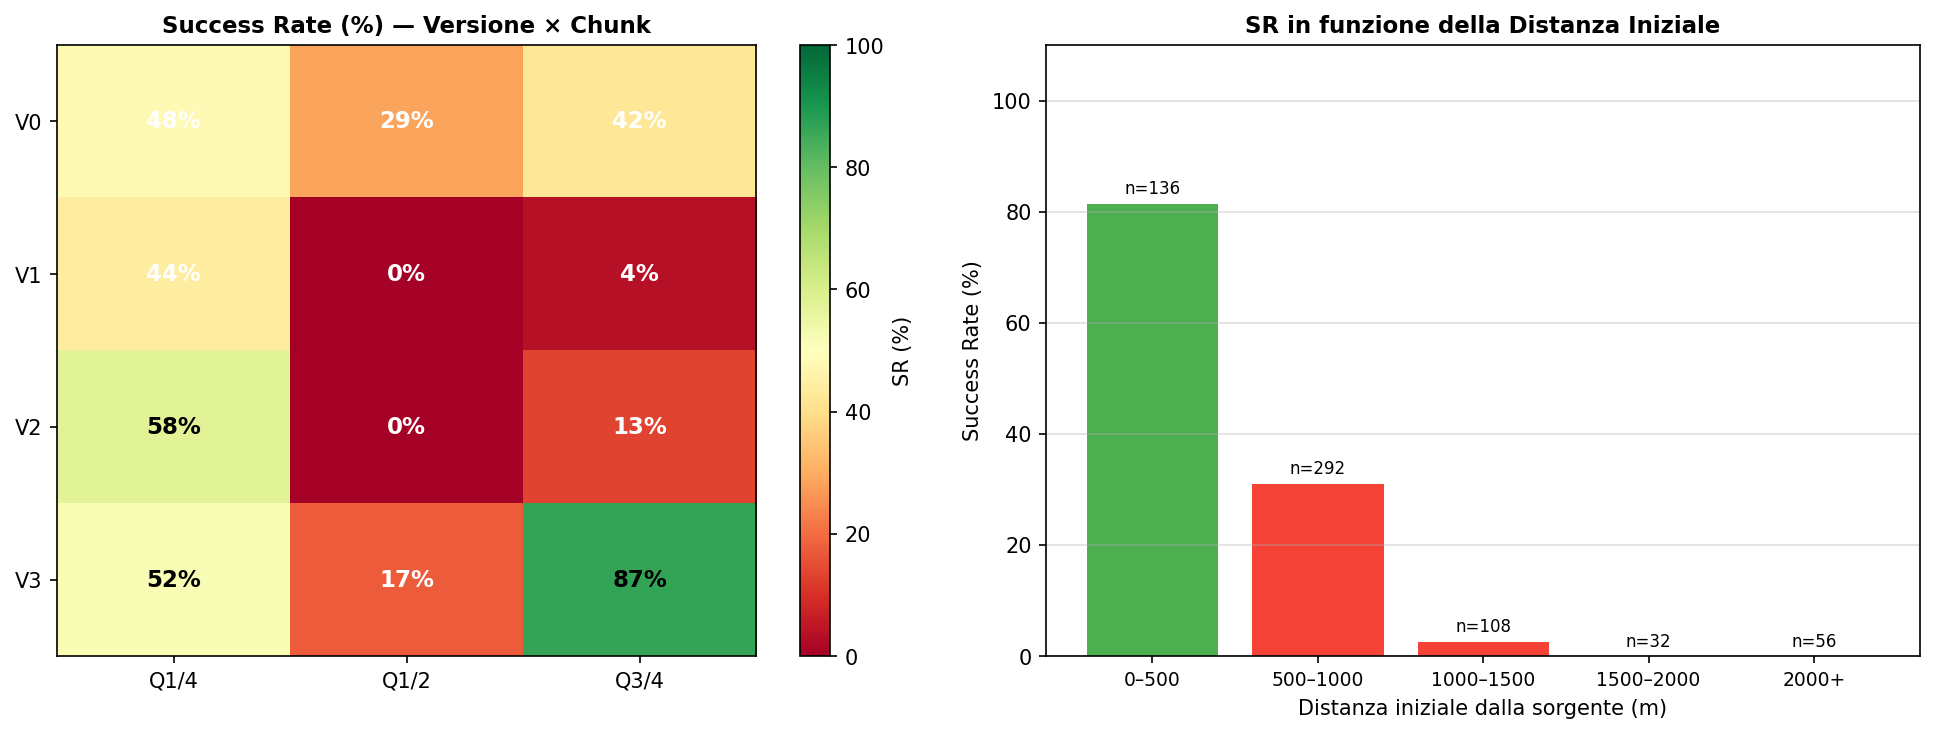
\includegraphics[width=0.97\linewidth]{fcmpure_sr_analysis.png}
  \caption{Success rate per scenario di vento e chunk temporale --- FCM puro
           $r_s = 50\,\text{m}$. Si evince che i fallimenti si concentrano negli scenari a
           plume diffuso (V1, V2) e nel chunk intermedio Q1/2, mentre V0/V3 e Q1/4 sono i
           pi\`u favorevoli.}
  \label{fig:fcmpure_sr}
\end{figure}

\begin{figure}[htbp]
  \centering
  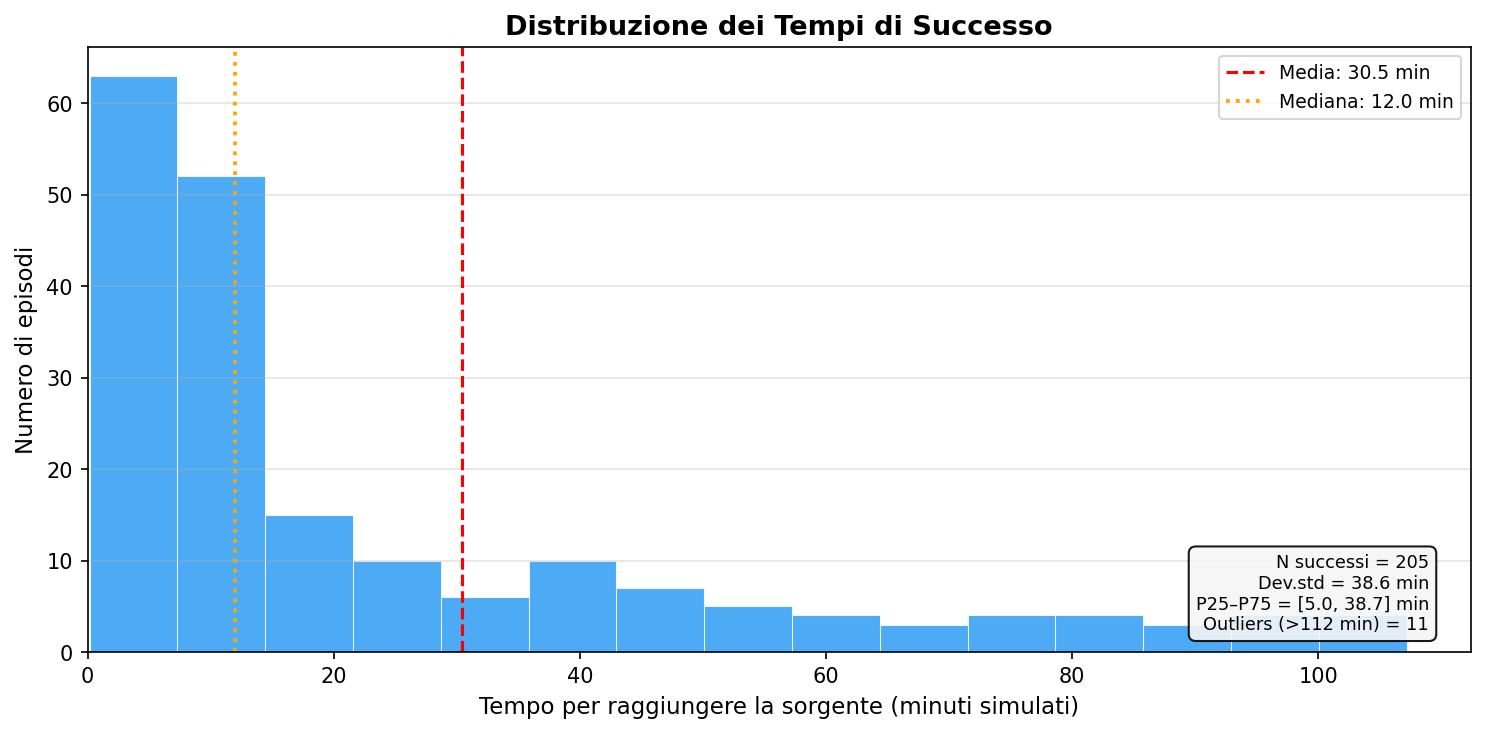
\includegraphics[width=0.97\linewidth]{fcmpure_success_time.png}
  \caption{Distribuzione del tempo al successo --- FCM puro $r_s = 50\,\text{m}$. La
           maggior parte dei successi avviene nei primi minuti, ma la coda lunga rivela
           numerosi episodi in cui l'agente vaga a lungo prima di convergere.}
  \label{fig:fcmpure_time}
\end{figure}

\begin{figure}[htbp]
  \centering
  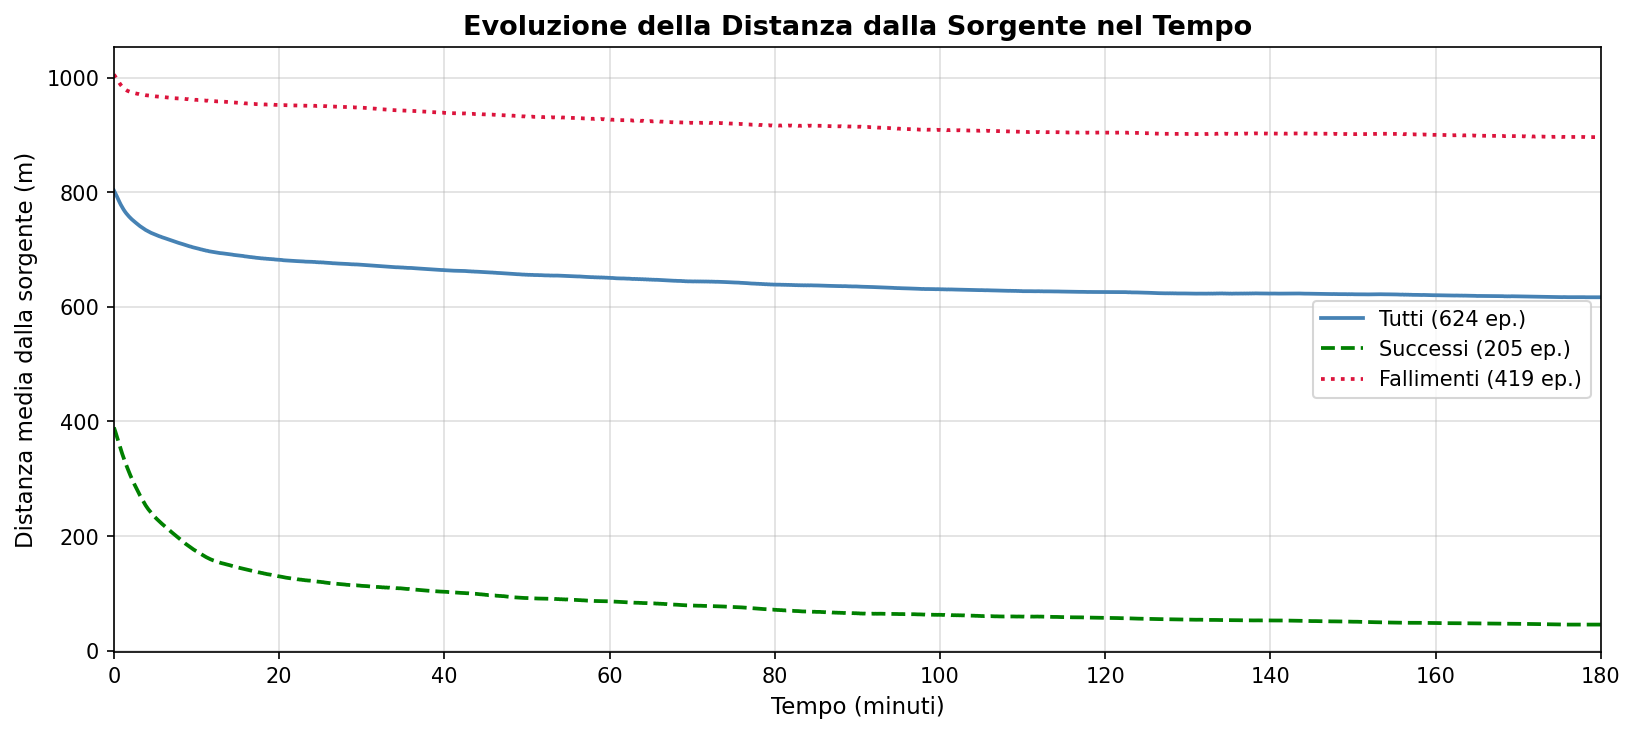
\includegraphics[width=0.97\linewidth]{fcmpure_distance_time.png}
  \caption{Distanza media dalla sorgente nel tempo --- FCM puro $r_s = 50\,\text{m}$. Gli
           episodi di successo riducono progressivamente la distanza, mentre i fallimenti
           restano stabili a grande distanza: il metodo reattivo entra in stallo senza
           riuscire ad avvicinarsi.}
  \label{fig:fcmpure_dist}
\end{figure}

\paragraph{Limiti del FCM puro.}
Anche al raggio ottimale, il success rate globale del FCM puro si ferma al $32{,}9\%$. La
causa principale \`e il \emph{passo fisso}, indipendente dalla storia del gradiente:
l'agente reagisce unicamente alla lettura corrente, senza memoria delle direzioni
percorse. In presenza di segnale rumoroso o plume diffuso ci\`o produce traiettorie
oscillanti e convergenza lenta, e il metodo tende a bloccarsi sui massimi locali di
concentrazione frequenti in ambiente costiero. Questi limiti motivano la variante
adattiva presentata nella sezione seguente.

% ════════════════════════════════════════════════════════════════════════════
\section{FCM con passo adattivo (Adam)}
\label{sec:fcm_adam}

Per superare i limiti del passo fisso, si sostituisce la regola di
selezione~\eqref{eq:argmax_fcm} con un aggiornamento basato sull'ottimizzatore
\textbf{Adam} (\emph{Adaptive Moment Estimation})~\citep{adam}. Adam accumula un
\emph{momentum} sul gradiente stimato e normalizza il passo per la varianza storica
del gradiente stesso, ottenendo un comportamento pi\`u robusto al rumore e pi\`u
direzionato.

Ad ogni timestep $t$ l'agente stima il gradiente locale
$\hat{\nabla}C_t \in \mathbb{R}^2$ tramite la~\eqref{eq:grad_ls} e calcola il
vettore di passo secondo la regola di aggiornamento Adam:
\begin{align}
    \mathbf{m}_t &= \beta_1\,\mathbf{m}_{t-1} + (1-\beta_1)\,\hat{\nabla}C_t \\
    \mathbf{v}_t &= \beta_2\,\mathbf{v}_{t-1} + (1-\beta_2)\,\hat{\nabla}C_t^{\,2} \\
    \hat{\mathbf{m}}_t &= \frac{\mathbf{m}_t}{1-\beta_1^t}, \qquad
    \hat{\mathbf{v}}_t = \frac{\mathbf{v}_t}{1-\beta_2^t} \\[4pt]
    \mathbf{s}_t &= lr \cdot \frac{\hat{\mathbf{m}}_t}{\sqrt{\hat{\mathbf{v}}_t} + \varepsilon}
    \label{eq:adam_step}
\end{align}

dove $\mathbf{m}_t, \mathbf{v}_t \in \mathbb{R}^2$ sono il primo e il secondo momento
del gradiente (inizializzati a $\mathbf{0}$ all'inizio di ogni episodio),
$\beta_1 = 0{,}9$, $\beta_2 = 0{,}999$, $\varepsilon = 10^{-8}$, e $lr$ \`e il
\emph{learning rate}, che rappresenta il passo base in metri. Il passo fisico effettivo
\`e limitato superiormente da $\Delta x_{\max} = 50\,\text{m}$, e l'azione discreta
viene scelta come la direzione $\hat{d}_i$ pi\`u allineata al vettore $\mathbf{s}_t$:
\begin{equation}
    \Delta x_t = \min\!\left(\left\|\mathbf{s}_t\right\|,\; \Delta x_{\max}\right),
    \qquad
    a_t = \operatorname*{argmax}_{i \in \{1,\ldots,8\}} \; \hat{d}_i \cdot \mathbf{s}_t
\end{equation}

Il momentum ($\beta_1$) mantiene la direzione coerente su pi\`u timestep, smorzando
le oscillazioni dovute al rumore del sensore; la normalizzazione per
$\sqrt{\hat{\mathbf{v}}_t}$ riduce il passo nelle direzioni in cui il gradiente \`e
inconsistente nel tempo. Lo pseudocodice dell'aggiornamento \`e riportato di seguito.

\begin{figure}[H]
\noindent\rule{\linewidth}{0.8pt}\vspace{-3pt}
\noindent\rule{\linewidth}{0.4pt}
\vspace{4pt}

\noindent\textit{FCM Adam: aggiornamento del passo per ogni timestep dell'episodio}

\vspace{4pt}
\noindent\rule{\linewidth}{0.4pt}
\vspace{4pt}

\small
\begin{tabbing}
\hspace{2.2em}\=\hspace{2.2em}\=\kill
\textit{--- Inizio episodio ---}\\[4pt]
$\mathbf{m} = \mathbf{0}_2$;\quad $\mathbf{v} = \mathbf{0}_2$;\quad $t = 0$;\\[8pt]
\textit{--- Per ogni timestep ---}\\[4pt]
$\hat{\nabla}C$ = stima\_gradiente(obs);\quad\textit{(minimi quadrati, 8 sensori)}\\[4pt]
$t = t + 1$;\\[4pt]
$\mathbf{m} = \beta_1 \cdot \mathbf{m} + (1 - \beta_1) \cdot \hat{\nabla}C$;\\[4pt]
$\mathbf{v} = \beta_2 \cdot \mathbf{v} + (1 - \beta_2) \cdot \hat{\nabla}C^{\,2}$;\\[6pt]
$\hat{\mathbf{m}} = \mathbf{m}\;/\;(1 - \beta_1^{\,t})$;\quad
$\hat{\mathbf{v}} = \mathbf{v}\;/\;(1 - \beta_2^{\,t})$;\\[6pt]
$\mathbf{s} = lr \cdot \hat{\mathbf{m}}\;/\;(\sqrt{\hat{\mathbf{v}}} + \varepsilon)$;\\[4pt]
$\Delta x = \min(\|\mathbf{s}\|,\; \Delta x_{\max})$;\\[4pt]
$a = \operatorname{argmax}_i\;(\hat{d}_i \cdot \mathbf{s})$;
\end{tabbing}

\vspace{2pt}
\noindent\rule{\linewidth}{0.4pt}\vspace{-3pt}
\noindent\rule{\linewidth}{0.8pt}
\end{figure}

Concretamente, ad ogni timestep la selezione dell'azione si traduce in:

\begin{lstlisting}
self.t += 1
self.m = b1 * self.m + (1 - b1) * grad           # primo momento
self.v = b2 * self.v + (1 - b2) * grad**2         # secondo momento
m_hat = self.m / (1 - b1**self.t)                 # bias correction
v_hat = self.v / (1 - b2**self.t)
step  = lr * m_hat / (np.sqrt(v_hat) + eps)       # vettore di passo Adam
action = int(np.argmax(D @ step))                 # direzione piu' allineata
\end{lstlisting}

\subsection{Interpretazione del learning rate}

Il parametro $lr$ rappresenta il passo asintotico per direzioni cardinali del
gradiente: a convergenza dei momenti Adam, $\|\mathbf{s}_t\| \to lr$ per gradienti
puramente orizzontali o verticali, e fino a $lr\sqrt{2}$ per gradienti diagonali
(comunque limitato a $\Delta x_{\max}$). Con $\Delta t = 10\,\text{s}$, un passo di
$lr = 10\,\text{m}$ corrisponde a una velocit\`a di $1\,\text{m/s}$, compatibile con la
velocit\`a nominale del veicolo; valori maggiori di $lr$ implicano velocit\`a
proporzionalmente pi\`u alte (fino a $5\,\text{m/s}$ per $lr = 50\,\text{m}$), a scapito
del realismo fisico.

\subsection{Analisi del learning rate e risultati}
\label{sec:fcm_lr}

Il parametro $lr$ \`e stato ottimizzato tramite uno sweep su
$lr \in \{10, 20, 30, 40, 50\}\,\text{m}$, con 624 episodi per valore e sensor range
$r_s = 50\,\text{m}$. La Tabella~\ref{tab:fcm_sweep} riporta il success rate globale, gli
step medi al successo e il dettaglio per scenario di vento e chunk temporale, confrontati
con la baseline a passo fisso ($10\,\text{m}$).

\begin{table}[H]
\centering
\renewcommand{\arraystretch}{1.05}
\resizebox{\linewidth}{!}{%
\setlength{\tabcolsep}{4pt}%
\begin{tabular}{C{1.5cm} C{1.0cm} C{1.5cm} C{1.0cm} C{1.0cm} C{1.0cm} C{1.0cm} C{1.0cm} C{1.0cm} C{1.0cm}}
\toprule
\rowcolor{headerbg}
\textcolor{white}{\textbf{$lr$}} &
\textcolor{white}{\textbf{SR\%}} &
\textcolor{white}{\textbf{Step medi}} &
\textcolor{white}{\textbf{V0}} &
\textcolor{white}{\textbf{V1}} &
\textcolor{white}{\textbf{V2}} &
\textcolor{white}{\textbf{V3}} &
\textcolor{white}{\textbf{Q1/4}} &
\textcolor{white}{\textbf{Q1/2}} &
\textcolor{white}{\textbf{Q3/4}} \\
\midrule
FCM puro & 32{,}9 & 182{,}7 & 39{,}7 & 16{,}0 & 23{,}7 & 51{,}9 & 50{,}5 & 11{,}5 & 36{,}5 \\
\rowcolor{rowalt}
10\,m & 54{,}6 & 174{,}0 & 73{,}7 & 29{,}5 & 35{,}9 & 79{,}5 & 77{,}9 & 30{,}3 & 55{,}8 \\
20\,m & 58{,}2 & 131{,}5 & 80{,}1 & 32{,}1 & 34{,}6 & 85{,}9 & 81{,}7 & 38{,}0 & 54{,}8 \\
\rowcolor{rowalt}
30\,m & 60{,}7 & 110{,}4 & 84{,}6 & 30{,}8 & 37{,}2 & 90{,}4 & 86{,}1 & 39{,}4 & 56{,}7 \\
\rowcolor{best}
\textbf{40\,m} & \textbf{63{,}5} & \textbf{115{,}1} & \textbf{84{,}6} & \textbf{35{,}3} & \textbf{41{,}7} & \textbf{92{,}3} & \textbf{90{,}9} & \textbf{44{,}2} & \textbf{55{,}3} \\
50\,m & 62{,}2 & 82{,}9 & 84{,}6 & 34{,}6 & 37{,}2 & 92{,}3 & 89{,}4 & 41{,}8 & 55{,}3 \\
\bottomrule
\end{tabular}}
\caption{Sweep su $lr$ per FCM Adam ($\beta_1{=}0{,}9$, $\beta_2{=}0{,}999$,
         $\Delta x_{\max}{=}50\,\text{m}$, $r_s{=}50\,\text{m}$, 624 episodi per valore).
         In verde la configurazione con il success rate pi\`u alto.}
\label{tab:fcm_sweep}
\end{table}

Il FCM Adam con $lr = 40\,\text{m}$ raggiunge il success rate globale pi\`u alto,
\textbf{63{,}5\%}, con un guadagno di \textbf{+30{,}6 punti percentuali} rispetto al
FCM puro a passo fisso (32{,}9\%). Il success rate \textbf{non cresce indefinitamente}
con $lr$: sale da $54{,}6\%$ ($lr = 10\,\text{m}$) fino al massimo a $40\,\text{m}$, per
poi ripiegare leggermente a $62{,}2\%$ a $50\,\text{m}$. Esiste dunque un passo ottimale,
oltre il quale falcate troppo ampie iniziano a scavalcare la struttura del plume anzich\'e
seguirla. Il miglioramento rispetto al FCM puro \`e comunque diffuso su tutti gli scenari,
con V3 e Q1/4 che beneficiano maggiormente del momentum, mentre V1, V2 e Q1/2 restano i
pi\`u critici.

Gli step medi al successo calano complessivamente all'aumentare di $lr$ (da 174 a 83):
passi pi\`u ampi riducono il numero di timestep necessari a raggiungere la sorgente.
L'andamento non \`e per\`o regolare --- a $lr = 40\,\text{m}$ gli step risalgono a
$115{,}1$ contro i $110{,}4$ di $30\,\text{m}$ --- e la spiegazione pi\`u naturale \`e un
effetto di \emph{selezione}: \`e proprio a $40\,\text{m}$ che il metodo porta a termine il
maggior numero di episodi, inclusi quelli difficili e lunghi che alle altre configurazioni
finivano in timeout e non entravano nella media. Un success rate pi\`u alto include
successi pi\`u faticosi, e la media degli step ne risente.

Si ricorda infine (Sezione~\ref{sec:fcm_adam}) che valori elevati di $lr$ comportano
velocit\`a non realistiche: il valore $lr = 10\,\text{m}$, fisicamente compatibile con la
velocit\`a nominale del veicolo, raggiunge gi\`a il $54{,}6\%$ di SR.

\paragraph{Comparabilit\`a degli spawn.} Va segnalato che il FCM puro e il FCM adattivo non
condividono lo stesso algoritmo di inizializzazione (Sezione~\ref{sec:spawn}): il primo, a
passo fisso, adotta la \emph{cascata di anelli} (distanza media di spawn $\sim$800\,m),
mentre il secondo, a passo variabile, adotta il \emph{disco adattivo}, che produce spawn in
media pi\`u vicini alla sorgente. Una parte del divario fra le due varianti riflette quindi
la diversa distribuzione delle distanze iniziali, e non il solo effetto dell'ottimizzatore
Adam. Il confronto pi\`u rigoroso, a parit\`a di condizioni, \`e quello fra RL e FCM adattivo
alla stessa velocit\`a massima (Sezione~\ref{sec:rl_fullrange}), in cui entrambi i metodi
condividono il disco adattivo.

Le Figure~\ref{fig:fcm_sr}--\ref{fig:fcm_dist} analizzano il comportamento del modello
migliore ($lr = 40\,\text{m}$) sui 624 episodi.

\begin{figure}[H]
  \centering
  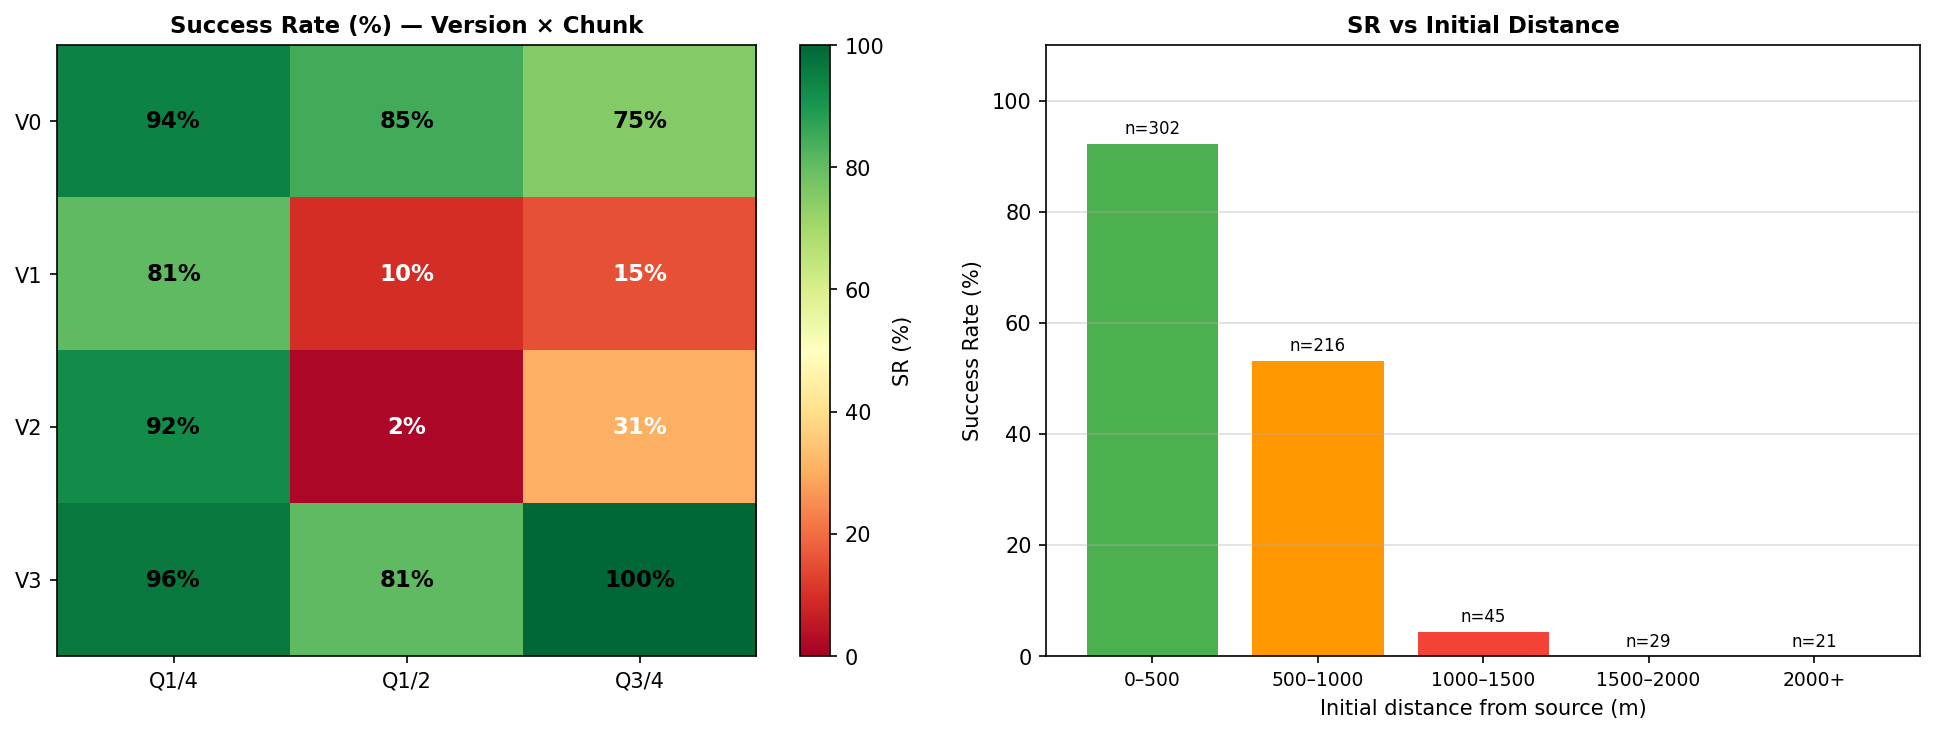
\includegraphics[width=0.97\linewidth]{plot_sr_analysis.png}
  \caption{Success rate per scenario di vento e chunk temporale --- FCM Adam
           $lr = 40\,\text{m}$. Rispetto al FCM puro il miglioramento \`e diffuso su tutti
           gli scenari, ma V1, V2 e Q1/2 rimangono i pi\`u critici: il momentum mitiga ma
           non elimina la difficolt\`a del plume diffuso.}
  \label{fig:fcm_sr}
\end{figure}

\begin{figure}[H]
  \centering
  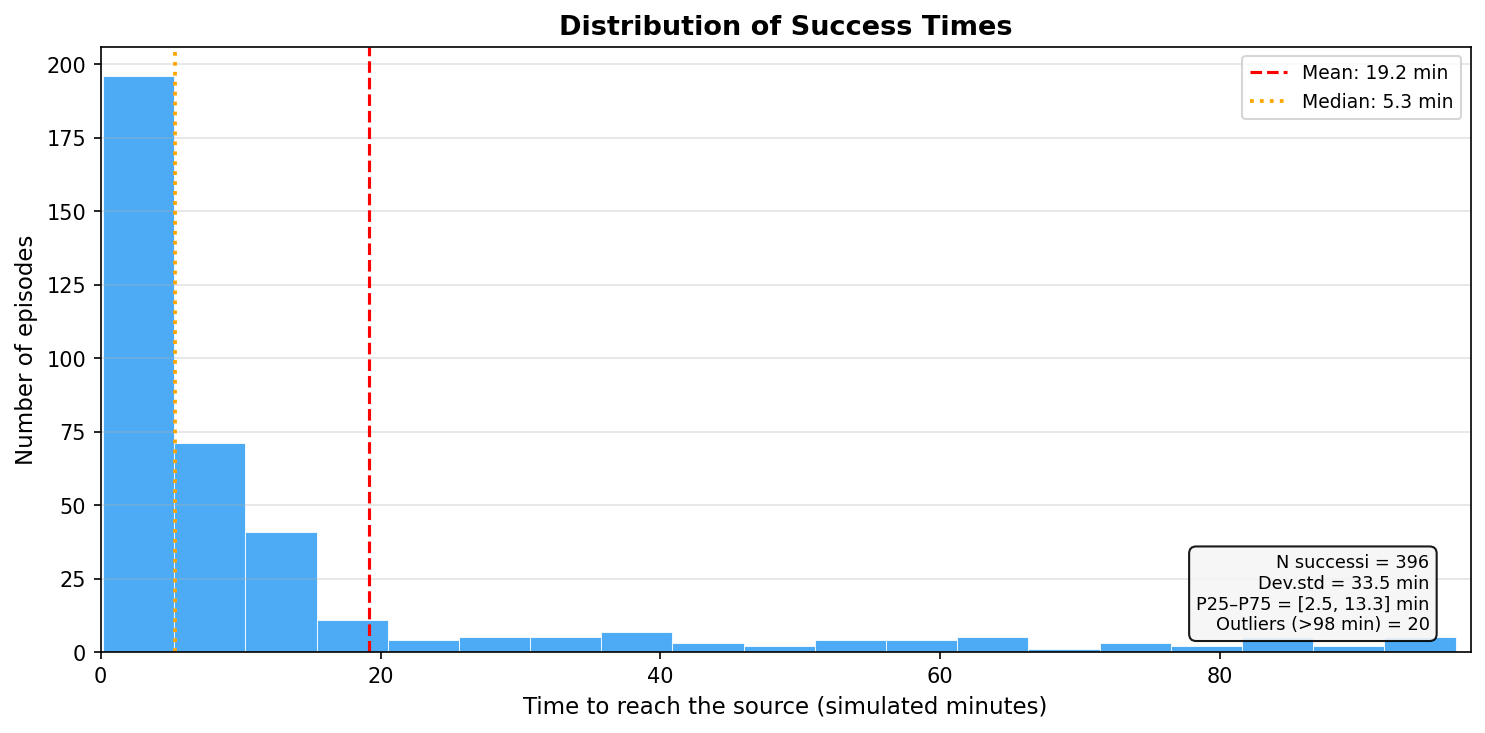
\includegraphics[width=0.97\linewidth]{plot_success_time_dist.png}
  \caption{Distribuzione del tempo al successo --- FCM Adam $lr = 40\,\text{m}$. La
           distribuzione \`e pi\`u concentrata sui tempi brevi rispetto al FCM puro: il
           passo adattivo riduce il numero di timestep necessari a raggiungere la
           sorgente.}
  \label{fig:fcm_time}
\end{figure}

\begin{figure}[H]
  \centering
  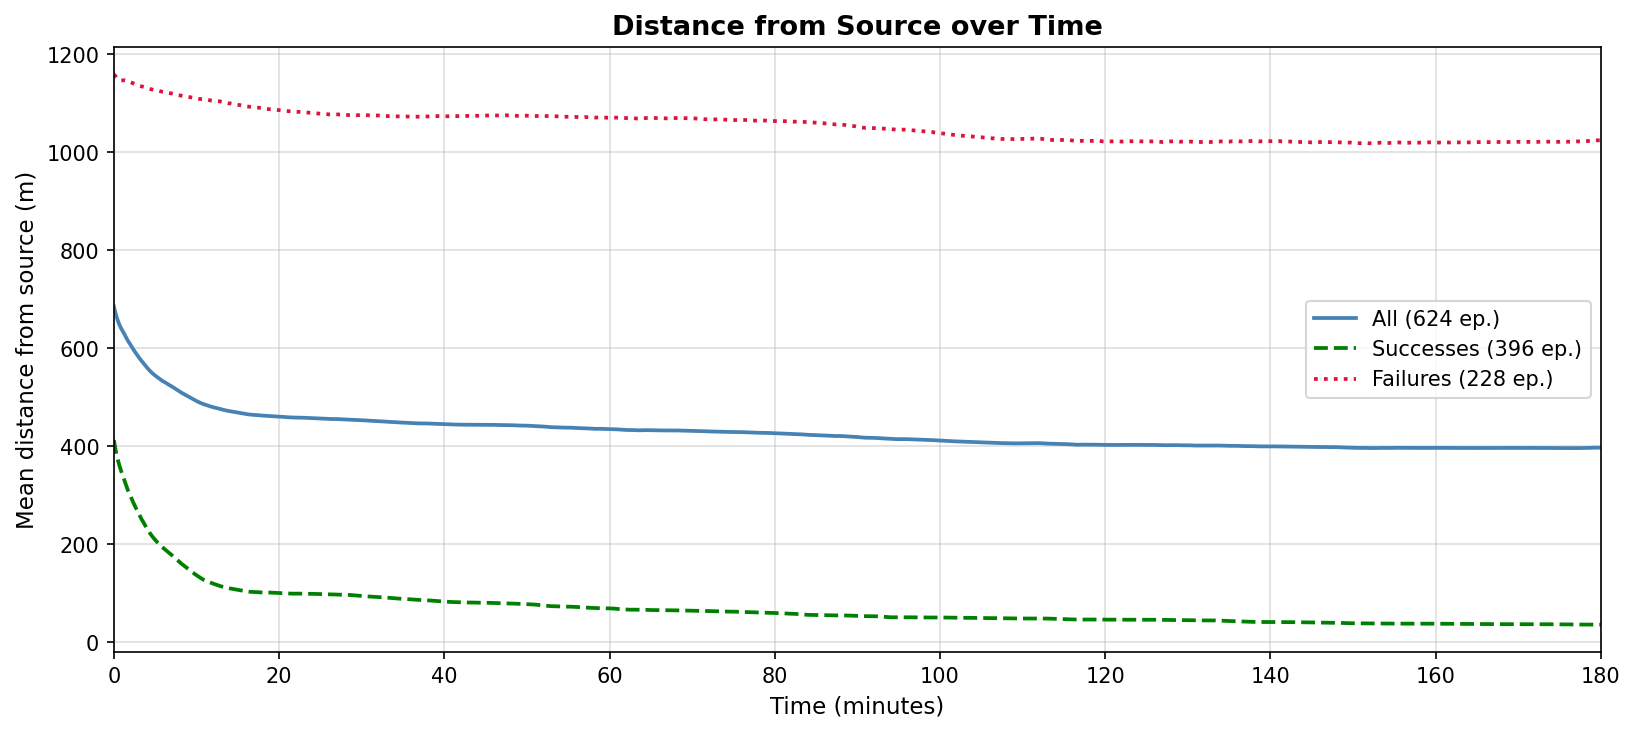
\includegraphics[width=0.97\linewidth]{plot_distance_over_time.png}
  \caption{Distanza media dalla sorgente nel tempo --- FCM Adam $lr = 40\,\text{m}$. La
           curva dei successi cala pi\`u rapidamente che nel FCM puro; resta comunque una
           quota di fallimenti stabili a grande distanza negli scenari pi\`u difficili.}
  \label{fig:fcm_dist}
\end{figure}

La Figura~\ref{fig:fcm_traj} mostra due episodi rappresentativi, tratti dalla
configurazione $lr = 50\,\text{m}$: un successo in condizioni di plume compatto (V0) e un
fallimento in condizioni di plume disperso (V2). Nel caso di fallimento, il campo diffuso
annulla il gradiente locale e l'agente non riesce a mantenere una direzione affidabile
verso la sorgente, terminando in timeout --- un limite qualitativo della risalita di
gradiente che non dipende dal particolare valore di $lr$.

\begin{figure}[H]
  \centering
  \begin{subfigure}{0.74\textwidth}
    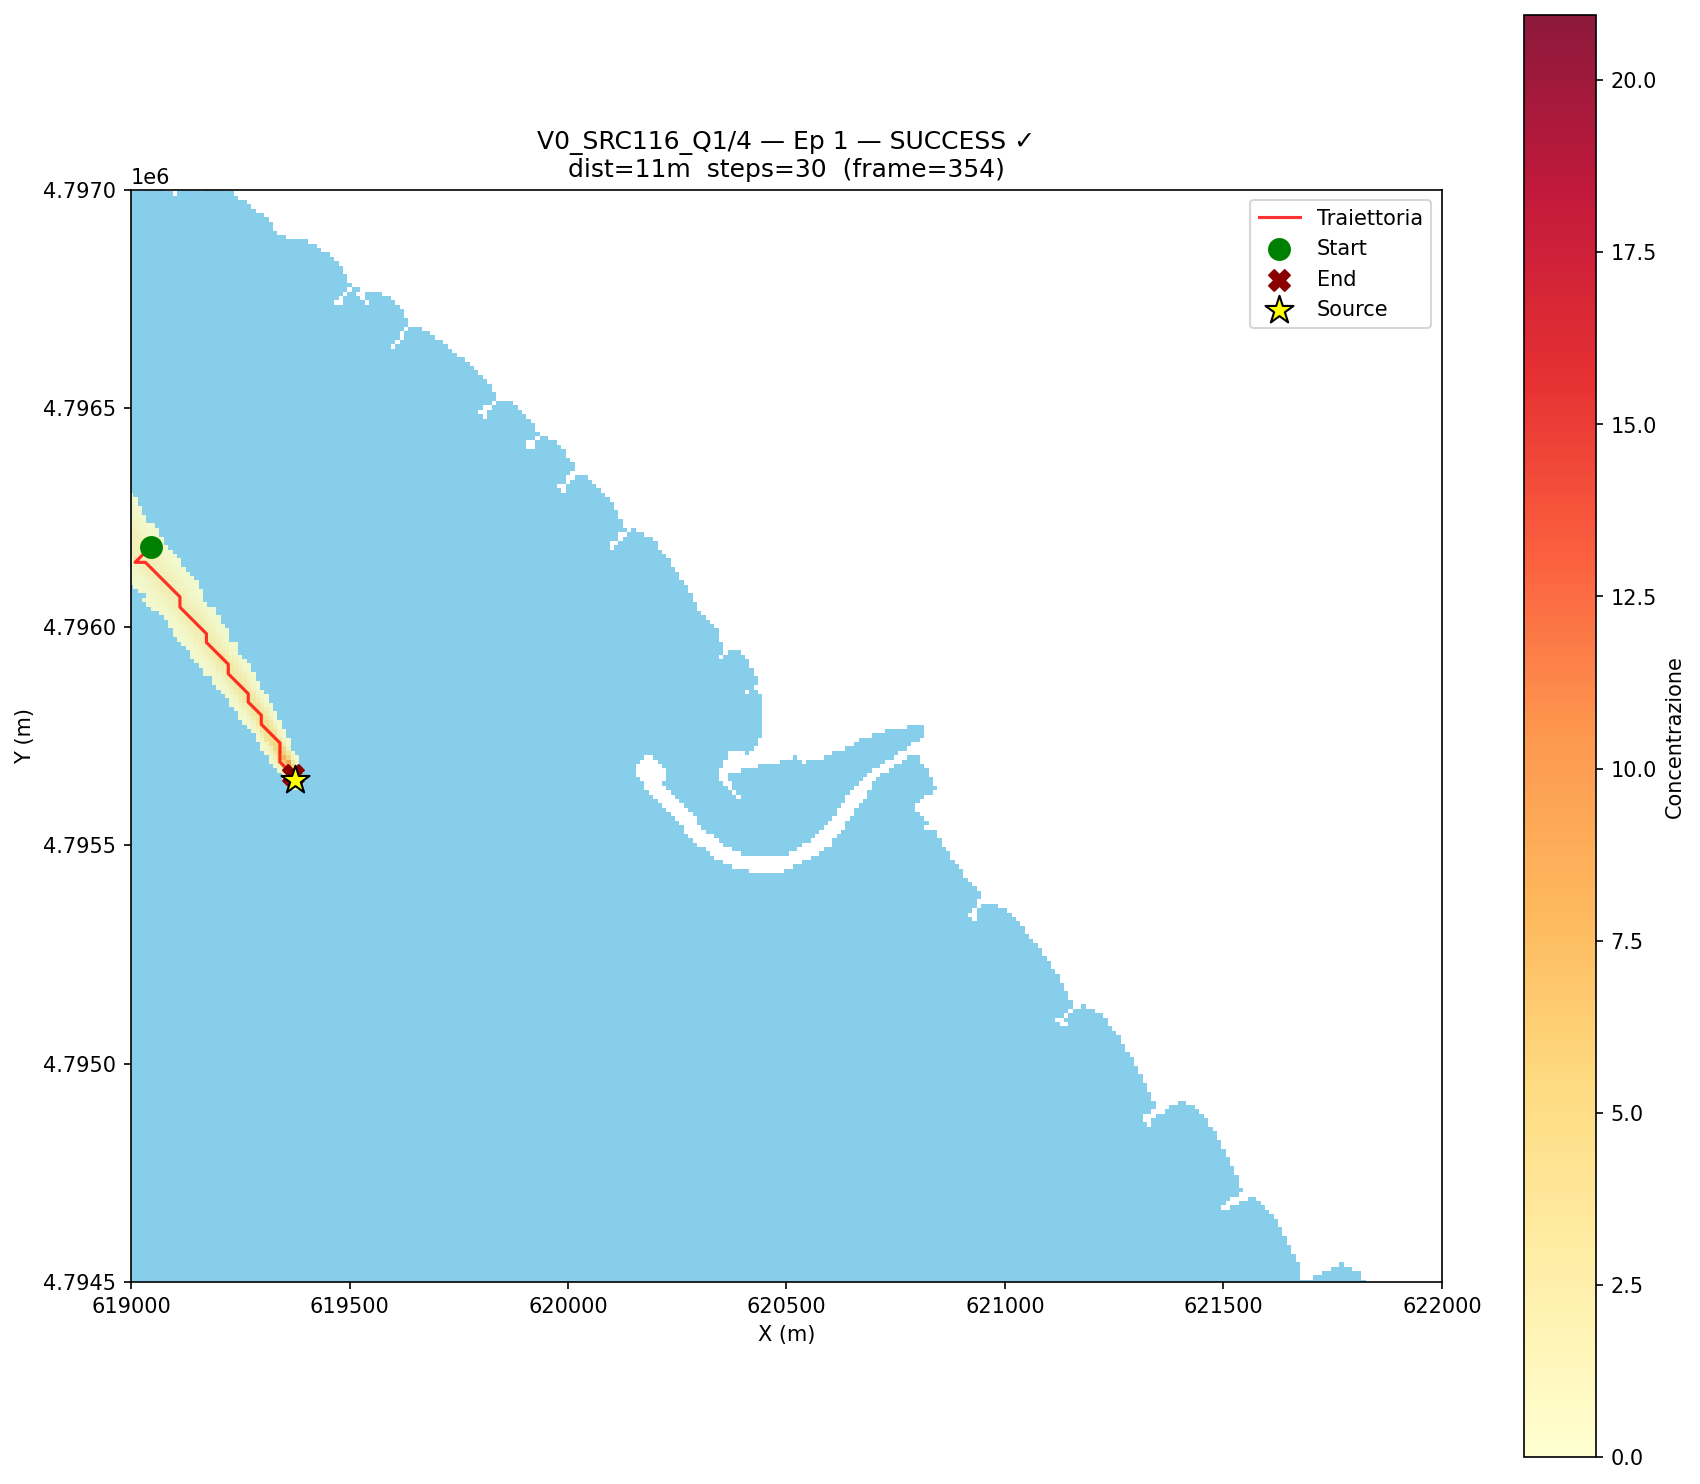
\includegraphics[width=\linewidth]{fcm_success_traj.png}
    \caption{Successo (V0, plume compatto).}
  \end{subfigure}

  \vspace{4mm}
  \begin{subfigure}{0.74\textwidth}
    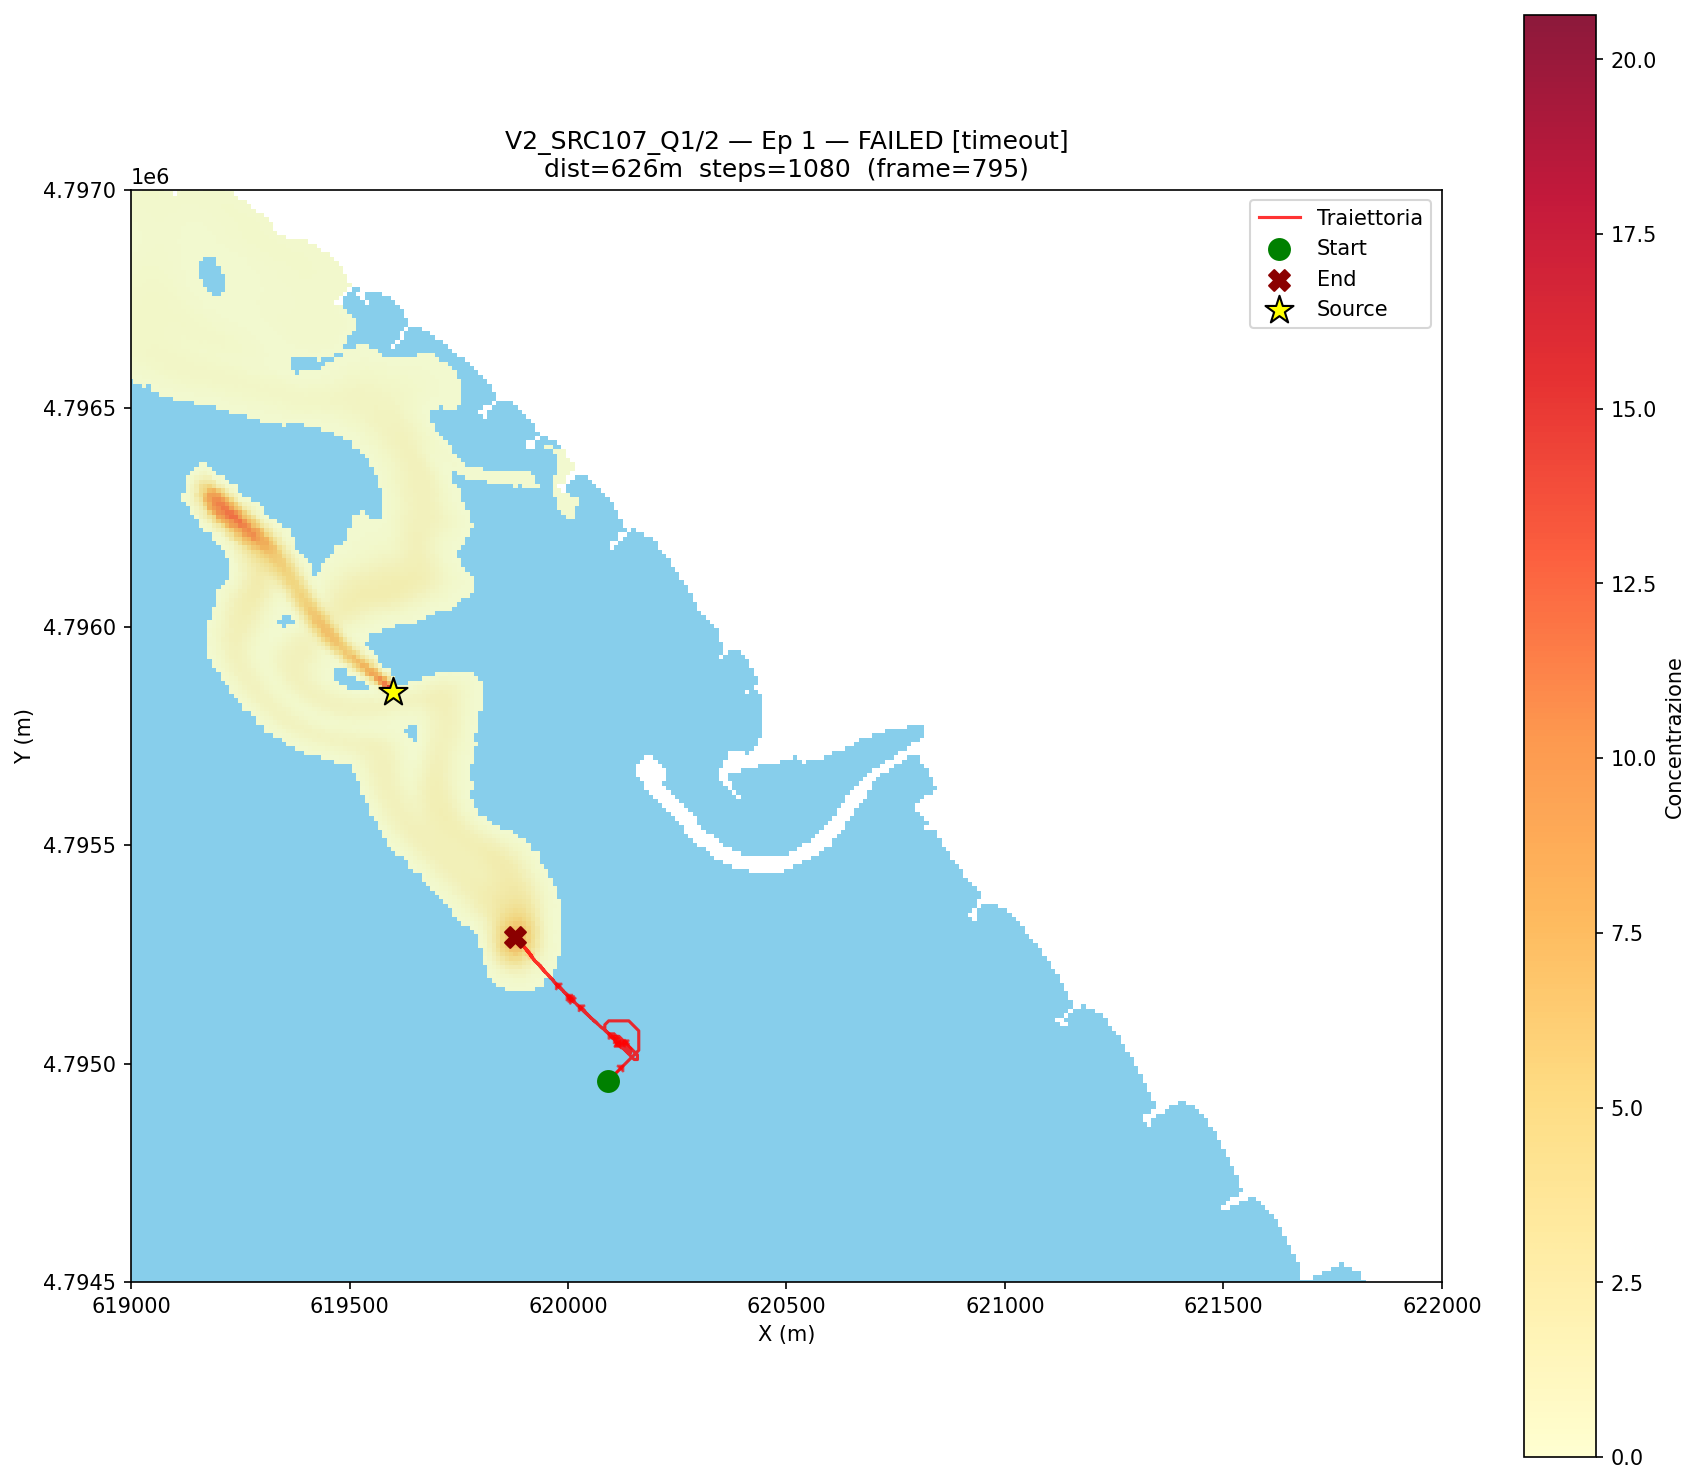
\includegraphics[width=\linewidth]{fcm_failure_traj.png}
    \caption{Fallimento (V2, plume disperso).}
  \end{subfigure}
  \caption{Traiettorie rappresentative del FCM Adam $lr = 50\,\text{m}$. Nel successo
           (a) l'agente risale il plume compatto con traiettoria diretta; nel fallimento
           (b) il plume disperso annulla il gradiente locale e l'agente vaga senza
           convergere, terminando in timeout.}
  \label{fig:fcm_traj}
\end{figure}

In sintesi, il metodo del gradiente adattivo migliora sensibilmente la baseline a passo
fisso, ma resta limitato dalla sua natura reattiva: negli scenari a plume diffuso
(V1, V2, Q1/2) il gradiente locale degenera e il success rate rimane basso. Questo
limite strutturale motiva l'approccio basato su Reinforcement Learning presentato nel
capitolo seguente.
             % Cap. 4 --- Metodo del gradiente: FCM
\chapter{Apprendimento per rinforzo: PPO}
\label{cap:rl}

\section{Motivazione}
\label{sec:rl_motiv}

Il metodo del gradiente presentato nel Capitolo~\ref{cap:fcm} \`e per natura
\emph{locale e reattivo}: decide l'azione basandosi solo sulle letture correnti degli
slave, senza memoria dell'episodio n\'e capacit\`a di pianificazione. Anche nella sua
versione adattiva con Adam, esso resta limitato negli scenari a plume diffuso, dove il
gradiente locale degenera e il metodo si blocca su massimi locali.

L'approccio proposto in questo lavoro si basa sul \textbf{Reinforcement Learning} (RL),
che mira a superare questi limiti apprendendo, tramite l'interazione ripetuta con
l'ambiente~\citep{sutton_barto}, una politica di navigazione che sfrutta la storia delle
osservazioni e le informazioni contestuali sul vento e sulle correnti. A differenza degli
approcci gradient-based e model-based, l'RL \`e \emph{model-free} e non richiede un
modello esplicito dell'ambiente: la strategia emerge dall'ottimizzazione su milioni di
episodi simulati. L'obiettivo \`e apprendere la politica del master a partire dalle stesse
misurazioni della squadra di slave usate dal FCM, verificando se l'apprendimento
produca strategie pi\`u robuste del gradiente reattivo.

\section{Introduzione a PPO}
\label{sec:ppo}

Proximal Policy Optimization (PPO)~\citep{ppo} \`e un algoritmo di reinforcement
learning \emph{on-policy} appartenente alla famiglia dei \emph{Policy Gradient Methods}.
L'architettura segue lo schema \emph{actor-critic}: una rete (la \emph{policy} o attore)
produce la distribuzione di probabilit\`a sulle azioni $\pi_\theta(a|s)$, mentre una
seconda rete (la \emph{value function} o critico) stima la funzione valore $V(s)$, ovvero
il \emph{ritorno atteso} (la somma scontata delle ricompense future) a partire dallo
stato $s$ seguendo la politica corrente.

In forma esplicita: poich\'e lo spazio d'azione di questo lavoro \`e \emph{discreto},
l'attore produce un vettore di \emph{logit} $z_\theta(s)$ e la politica \`e la distribuzione
categorica ottenuta con la funzione \emph{softmax},
\begin{equation}
    \pi_\theta(a \mid s) = \frac{\exp\!\big(z_\theta(s)_a\big)}
                                {\sum_{a'} \exp\!\big(z_\theta(s)_{a'}\big)},
    \label{eq:policy_softmax}
\end{equation}
mentre la funzione valore \`e definita come il ritorno atteso scontato a partire da $s$,
\begin{equation}
    V^{\pi_\theta}(s) = \mathbb{E}_{\pi_\theta}\!\left[\,
        \sum_{k=0}^{\infty} \gamma^{k}\, r_{t+k+1} \;\middle|\; s_t = s \right],
    \label{eq:value_fn}
\end{equation}
con $\gamma \in (0,1]$ il fattore di sconto (Tabella~\ref{tab:hyper}) e $r_{t}$ la ricompensa
al passo $t$; il critico ne apprende un'approssimazione $V_\phi(s)$ tramite una seconda rete.

Il meccanismo chiave di PPO \`e il \emph{clipped surrogate objective}: l'algoritmo
massimizza il miglioramento della policy ma limita la deviazione rispetto alla policy
precedente tramite il clipping del rapporto di probabilit\`a
$r_t(\theta) = \pi_\theta(a_t|s_t) / \pi_{\theta_{\text{old}}}(a_t|s_t)$:
\begin{equation}
    L^{\text{CLIP}}(\theta) = \mathbb{E}_t\!\left[\min\!\big(
    r_t(\theta)\,\hat{A}_t,\;
    \text{clip}(r_t(\theta), 1-\epsilon, 1+\epsilon)\,\hat{A}_t \big)\right]
    \label{eq:ppo_clip}
\end{equation}

dove $\hat{A}_t$ \`e la stima del vantaggio (\emph{advantage}) e $\epsilon$ \`e il
parametro di clipping. L'obiettivo complessivo combina tre contributi: la \emph{policy
loss} (clipped), la \emph{value loss} che allinea la stima $V(s)$ ai ritorni osservati, e
un termine di \emph{entropy bonus} che mantiene l'esplorazione:
\begin{equation}
    L(\theta) = L^{\text{CLIP}}(\theta) - c_1\,L^{\text{VF}}(\theta) + c_2\,H[\pi_\theta]
\end{equation}

La stima del vantaggio \`e ottenuta tramite \emph{Generalized Advantage Estimation}
(GAE)~\citep{gae}, che offre un buon compromesso tra bias e varianza. Durante il training
la policy \`e stocastica (campionamento da $\pi_\theta$); in inferenza pu\`o essere resa
deterministica scegliendo l'azione a probabilit\`a massima.

\subsection{MaskablePPO}
\label{sec:maskable}

L'implementazione utilizzata \`e \textbf{MaskablePPO} della libreria \emph{sb3-contrib},
estensione di PPO che integra l'\emph{action masking}~\citep{maskable_ppo} descritto nella
Sezione~\ref{sec:masking}. Ad ogni passo, le azioni che porterebbero il master sulla
terraferma o fuori dal dominio vengono escluse dalla distribuzione di probabilit\`a,
impedendo le collisioni con la costa senza penalit\`a a posteriori e garantendo
l'esplorazione di sole traiettorie ammissibili.

L'architettura della policy \`e una rete \emph{Multi-Layer Perceptron} (MLP) con due reti
separate per attore e critico, ciascuna composta da due strati nascosti da 256 neuroni
con attivazione $\tanh$. La libreria \emph{Stable-Baselines3}~\citep{sb3}, costruita su
PyTorch, fornisce l'implementazione di base e ne rende l'uso riproducibile. La creazione
dell'agente e l'avvio dell'addestramento si riducono a poche righe:

\begin{lstlisting}
env = ActionMasker(SourceSeekingEnv(config), mask_fn)   # masking delle azioni
model = MaskablePPO("MlpPolicy", env,
                    policy_kwargs=dict(net_arch=[256, 256], activation_fn=nn.Tanh),
                    n_steps=4096, batch_size=128, gamma=0.99, clip_range=0.15)
model.learn(total_timesteps=6_000_000)
\end{lstlisting}

\section{Spazio di osservazione}
\label{sec:osservazione}

L'osservazione fornita alla rete neurale rappresenta il campo chimico locale, la
cinematica dell'agente e le condizioni ambientali. Tutte le feature sono normalizzate.
Se ne considerano due configurazioni, confrontate nella
Sezione~\ref{sec:rl_dual}: la \textbf{singola corona} (\textbf{116 dimensioni}), in cui
gli slave formano un'unica corona di 8 sensori a $r_s = 20\,\text{m}$ attorno al master,
e la \textbf{doppia corona} (\textbf{196 dimensioni}), che aggiunge una seconda corona a
$r_{s2} = 50\,\text{m}$ per dare all'agente informazione sul plume a scala spaziale
pi\`u larga. La struttura \`e riportata nella Tabella~\ref{tab:obs}.

\begin{table}[H]
\centering
\renewcommand{\arraystretch}{1.25}
\small
\begin{tabular}{L{5.0cm} C{1.5cm} C{1.5cm} L{4.6cm}}
\toprule
\rowcolor{headerbg}
\textcolor{white}{\textbf{Componente}} &
\textcolor{white}{\textbf{Singola}} &
\textcolor{white}{\textbf{Doppia}} &
\textcolor{white}{\textbf{Descrizione}} \\
\midrule
Concentrazione corrente        & 1  & 1  & Concentrazione nella posizione attuale \\
\rowcolor{rowalt}
Memoria concentrazione         & 9  & 9  & Ultime 9 letture di concentrazione \\
Memoria spostamenti            & 18 & 18 & Ultimi 9 spostamenti $(\Delta x, \Delta y)$ \\
\rowcolor{rowalt}
Sensori corona 1               & 8  & 8  & Concentrazione nelle 8 direzioni a $20\,\text{m}$ \\
Sensori corona 2               & -- & 8  & Concentrazione nelle 8 direzioni a $50\,\text{m}$ \\
\rowcolor{rowalt}
Memoria corona 1               & 72 & 72 & Corona 1 per i 9 timestep passati \\
Memoria corona 2               & -- & 72 & Corona 2 per i 9 timestep passati \\
\rowcolor{rowalt}
Vento                          & 2  & 2  & Componenti $u, v$ [m/s] \\
Corrente                       & 2  & 2  & Componenti $u, v$ [m/s] \\
\rowcolor{rowalt}
Informazione posizionale       & 4  & 4  & Direzione e valore della max concentrazione vista,
                                           step dall'ultimo contatto col plume \\
\midrule
\textbf{Totale}                & \textbf{116} & \textbf{196} & \\
\bottomrule
\end{tabular}
\caption{Spazio di osservazione della rete neurale: singola corona (116 dimensioni) e
         doppia corona (196 dimensioni).}
\label{tab:obs}
\end{table}

\section{Addestramento}
\label{sec:training}

I modelli sono addestrati per $6 \times 10^6$ step con gli iperparametri riportati nella
Tabella~\ref{tab:hyper}, sulla suddivisione del dataset e con l'augmentation temporale
descritte nella Sezione~\ref{sec:split}.

\paragraph{Learning rate decrescente.}
Il learning rate segue uno \textbf{schedule a gradini decrescenti}
(Tabella~\ref{tab:lr_curr}, sinistra): si parte da un valore relativamente alto
($3 \times 10^{-4}$) nelle prime fasi, quando la policy \`e ancora lontana
dall'ottimo e conviene compiere aggiornamenti ampi per esplorare rapidamente lo spazio
delle soluzioni, e lo si riduce progressivamente fino a $1 \times 10^{-5}$ nelle fasi
finali, quando servono aggiustamenti pi\`u fini per affinare la politica senza
destabilizzare quanto gi\`a appreso.

\paragraph{Curriculum sugli scenari.}
La distribuzione degli scenari di addestramento evolve tramite un parametro
$\alpha \in [0,1]$ (Tabella~\ref{tab:lr_curr}, destra): per $\alpha = 0$ gli scenari sono
estratti in modo \textbf{uniforme}, mentre per $\alpha \to 1$ il peso si concentra
progressivamente sugli scenari pi\`u difficili --- lo scenario di vento V2 e i chunk
temporali centrali (Q1/2), caratterizzati da plume pi\`u diffuso. In questo modo l'agente
apprende prima le situazioni pi\`u semplici e, una volta acquisita una politica di base,
viene esposto in misura crescente ai casi critici, secondo la logica del
\emph{curriculum learning}.

\begin{table}[H]
\centering
\small
\begin{minipage}{0.48\linewidth}
\centering
\renewcommand{\arraystretch}{1.2}
\begin{tabular}{C{3.5cm} C{2cm}}
\toprule
\rowcolor{headerbg}
\textcolor{white}{\textbf{Step}} & \textcolor{white}{\textbf{LR}} \\
\midrule
0 -- 2\,000\,000        & $3 \times 10^{-4}$ \\
2\,000\,000 -- 4\,000\,000 & $1 \times 10^{-4}$ \\
4\,000\,000 -- 5\,000\,000 & $5 \times 10^{-5}$ \\
5\,000\,000 -- 6\,000\,000 & $1 \times 10^{-5}$ \\
\bottomrule
\end{tabular}
\end{minipage}
\hfill
\begin{minipage}{0.48\linewidth}
\centering
\renewcommand{\arraystretch}{1.2}
\begin{tabular}{C{3.5cm} C{2cm}}
\toprule
\rowcolor{headerbg}
\textcolor{white}{\textbf{Step}} & \textcolor{white}{\textbf{$\alpha$}} \\
\midrule
0 -- 2\,000\,000        & 0{,}0 \\
2\,000\,000 -- 4\,000\,000 & 0{,}5 \\
4\,000\,000 -- 6\,000\,000 & 0{,}8 \\
\bottomrule
\end{tabular}
\end{minipage}
\caption{Schedule del learning rate (sinistra) e curriculum sugli scenari (destra).}
\label{tab:lr_curr}
\end{table}

\begin{table}[H]
\centering
\renewcommand{\arraystretch}{1.2}
\small
\begin{tabular}{L{5cm} C{4cm}}
\toprule
\rowcolor{headerbg}
\textcolor{white}{\textbf{Parametro}} & \textcolor{white}{\textbf{Valore}} \\
\midrule
Algoritmo            & MaskablePPO \\
\rowcolor{rowalt}
Policy               & MLP ($256\times256$, $\tanh$) \\
Step totali          & $6\,000\,000$ \\
\rowcolor{rowalt}
$n\_steps$           & 4096 \\
Batch size           & 128 \\
\rowcolor{rowalt}
Epoche               & 10 \\
$\gamma$             & 0{,}99 \\
\rowcolor{rowalt}
$\lambda$ (GAE)      & 0{,}95 \\
Clip range           & 0{,}15 \\
\rowcolor{rowalt}
Coeff.\ value function & 0{,}3 \\
Coeff.\ entropia     & 0{,}01 \\
\rowcolor{rowalt}
Max grad norm        & 0{,}5 \\
Target KL            & 0{,}02 \\
\bottomrule
\end{tabular}
\caption{Iperparametri di training del modello PPO.}
\label{tab:hyper}
\end{table}

\section{Risultati}
\label{sec:rl_risultati}

La valutazione \`e condotta sulle 26 sorgenti held-out (SRC107--SRC132) su 4 scenari di
vento e 3 chunk temporali, in modalit\`a deterministica, per un totale di 1560 episodi
per modello. Si analizzano in sequenza l'effetto del raggio di campionamento
(Sezione~\ref{sec:rl_sensor}) e della funzione di reward (Sezione~\ref{sec:rl_reward}),
che fissano il modello di riferimento \texttt{minimal}. Da questo si sviluppa la
\textbf{catena a velocit\`a variabile} (Sezione~\ref{sec:rl_velocity}), in cui la
velocit\`a diventa una scelta dell'agente, e su ciascuno stadio della catena si valuta la
\textbf{doppia corona} (Sezione~\ref{sec:rl_dual}). Seguono due approfondimenti sulla
politica cos\`i ottenuta --- il restringimento del raggio di successo
(Sezione~\ref{sec:rl_r10}) e le heatmap di occupazione (Sezione~\ref{sec:rl_heatmap}) ---
quindi l'analisi delle spawn map (Sezione~\ref{sec:spawn_map}) e il confronto diretto con
il metodo del gradiente (Sezione~\ref{sec:rl_confronto}), esteso infine all'intero range di
velocit\`a operative (Sezione~\ref{sec:rl_fullrange}).

\subsection{Analisi sul raggio di campionamento crescente}
\label{sec:rl_sensor}

Analogamente a quanto fatto per l'FCM (Sezione~\ref{sec:sensor_range}), si \`e indagato
l'effetto del raggio di campionamento $r_s$ --- la distanza a cui gli slave si
posizionano attorno al master --- anche per l'agente RL. A partire da un modello base
addestrato con $r_s = 20\,\text{m}$ (success rate $94\%$), \`e stato condotto un
\emph{fine-tuning progressivo a catena} con raggi crescenti
$r_s \in \{50, 100, 150, 200\}\,\text{m}$: ogni modello \`e stato ottenuto rifinendo per
$2 \times 10^6$ step il modello dello stadio precedente
($20 \to 50 \to 100 \to 150 \to 200\,\text{m}$), con distribuzione uniforme di scenari e
chunk. La Tabella~\ref{tab:rl_sensor} riporta i risultati.

\begin{table}[H]
\centering
\renewcommand{\arraystretch}{1.3}
\resizebox{\linewidth}{!}{%
\setlength{\tabcolsep}{4pt}%
\begin{tabular}{C{1.6cm} C{1.0cm} C{1.0cm} C{1.0cm} C{1.0cm} C{1.0cm} C{1.0cm} C{1.0cm} C{1.0cm}}
\toprule
\rowcolor{headerbg}
\textcolor{white}{\textbf{$r_s$}} &
\textcolor{white}{\textbf{SR\%}} &
\textcolor{white}{\textbf{V0}} &
\textcolor{white}{\textbf{V1}} &
\textcolor{white}{\textbf{V2}} &
\textcolor{white}{\textbf{V3}} &
\textcolor{white}{\textbf{Q1/4}} &
\textcolor{white}{\textbf{Q1/2}} &
\textcolor{white}{\textbf{Q3/4}} \\
\midrule
\rowcolor{best}
\textbf{20\,m} & \textbf{94} & \textbf{100} & \textbf{82} & \textbf{87} & \textbf{99} & \textbf{100} & \textbf{84} & \textbf{96} \\
50\,m  & 93 & 100 & 82 & 91 & 100 & 100 & 84 & 96 \\
100\,m & 87 & 100 & 85 & 82 & 82 & 100 & 81 & 81 \\
150\,m & 63 & 65  & 60 & 61 & 66 & 61  & 56 & 72 \\
200\,m & 52 & 47  & 45 & 39 & 75 & 49  & 39 & 66 \\
\bottomrule
\end{tabular}}
\caption{Sweep sul raggio di campionamento per l'agente RL (fine-tuning progressivo dal
         modello base a $20\,\text{m}$, 1560 episodi per valore). In verde il valore
         ottimale.}
\label{tab:rl_sensor}
\end{table}

Si osserva una \textbf{degradazione monotona} delle prestazioni all'aumentare del raggio,
con il calo pi\`u netto tra 100\,m ($87\%$) e 150\,m ($63\%$). La spiegazione \`e di
natura fisica e coincide con quella dell'FCM: il criterio di successo richiede di arrivare
entro $50\,\text{m}$ dalla sorgente, un obiettivo di navigazione \emph{locale}; sensori
troppo distanti (es.\ $200\,\text{m}$) campionano punti oltre la sorgente stessa,
invertendo o annullando il gradiente direzionale nella fase critica di avvicinamento. Il
raggio ottimale per questo task e dataset \`e dunque $r_s \approx 20\,\text{m}$, fissato
dalla scala caratteristica del plume nelle simulazioni MIKE21; aumentarlo sostituisce
informazione locale utile con informazione irrilevante. Il risultato \`e indipendente
dall'architettura della rete e dalla funzione di reward, identiche per tutti i modelli
testati. Tutti i modelli successivi adottano quindi $r_s = 20\,\text{m}$.

\subsection{Analisi sulla funzione di reward}
\label{sec:rl_reward}

Fissato il raggio ottimale, si \`e studiato l'effetto della \textbf{funzione di reward}. Ad
ogni passo l'ambiente calcola una ricompensa scalare come \emph{somma} di pi\`u componenti;
le tre varianti confrontate differiscono per quali componenti sono attive e per la
\emph{forma} del termine di distanza. Se ne descrivono di seguito i singoli componenti.

\begin{itemize}[leftmargin=1.4em, itemsep=2pt]
  \item \textbf{Bonus di raggiungimento}: $+100$ all'arrivo (distanza $\leq 50\,$m), pi\`u un
        bonus di tempo residuo $\max\!\big(0,\,(N_{\max}-k)/N_{\max}\cdot 50\big)$ che premia
        l'arrivare in anticipo.
  \item \textbf{Penalit\`a di uscita dal dominio}: $-10$ se il passo porta fuori dai bordi.
  \item \textbf{Reward di distanza} (segnale dominante): premia l'avvicinamento alla sorgente.
        In forma \emph{lineare} \`e proporzionale alla riduzione di distanza nel passo,
        $(d_{t-1}-d_t)\,K/3000$; in forma \emph{quadratica} (variante \texttt{full}) usa un
        potenziale $\propto(Q-d)^2$ modulato da uno \emph{zone multiplier} (che pesa di pi\`u i
        progressi vicino alla sorgente) e da una \emph{retreat asymmetry} (il moto di
        allontanamento \`e penalizzato $3\times$).
  \item \textbf{Gradiente di concentrazione}: $\pm 0{,}05$ a seconda che la concentrazione
        sotto l'agente aumenti o diminuisca nel passo.
  \item \textbf{Allineamento a vento e corrente}: $\pm 0{,}05$ per ciascuno, che premia il
        muoversi \emph{controvento} e \emph{controcorrente} (assunti diretti verso la sorgente).
  \item \textbf{Penalit\`a di tempo}: $-0{,}1$ per passo, per incentivare la rapidit\`a.
  \item \textbf{Prossimit\`a alla costa}: rampa lineare da $0$ (a $30\,$m dalla terra) fino a
        $-15$ (sul bordo).
  \item \textbf{Stagnazione} (solo \texttt{full}): se in una finestra di passi la distanza
        minima non migliora abbastanza, una penalit\`a scoraggia il vagare; una variante
        \emph{direzionale} penalizza i percorsi in cui lo spostamento netto \`e piccolo
        rispetto a quello totale (moto inefficiente).
\end{itemize}

Le tre varianti si ottengono attivando o disattivando questi componenti (parametro
\texttt{reward\_mode}):
\begin{description}[leftmargin=1.4em, style=nextline]
    \item[\texttt{full}] tutti i componenti: distanza \emph{quadratica} con zone multiplier e
          retreat asymmetry, allineamento a vento/corrente e le penalit\`a di stagnazione.
    \item[\texttt{base}] distanza \emph{lineare} e simmetrica; rimossi zone multiplier, retreat
          asymmetry e stagnazione. Allineamento a vento e corrente ancora attivi.
    \item[\texttt{minimal}] come \texttt{base}, ma con l'allineamento a vento e corrente
          \emph{rimosso}. Restano i soli segnali essenziali: raggiungimento ($+100$), uscita
          dal dominio ($-10$), distanza lineare, gradiente di concentrazione ($\pm 0{,}05$),
          tempo ($-0{,}1$/step) e prossimit\`a alla costa. Nel codice questa variante
          corrisponde a \texttt{reward\_mode = "base\_no\_wind\_reward"}.
\end{description}

In codice, l'assemblaggio del reward e i punti in cui le varianti divergono sono:

\begin{lstlisting}
def _compute_reward(self):
    r = 0.0
    if self._source_reached():                    # 1) raggiungimento
        r += 100.0 + max(0, (N_max - k) / N_max * 50)   # (+ bonus di tempo)
    if self._out_of_bounds():                     # 2) fuori dominio
        r += -10.0
    r += self._distance_reward(d, d_prev)         # 3) distanza
    r += 0.05 if conc > prev_conc else -0.05      # 4) gradiente conc.
    if self.reward_mode != "base_no_wind_reward": # 5) allineamento (no in minimal)
        r += self._alignment_reward(v, wind, current)
    r += -0.1                                     # 6) tempo
    r += self._land_proximity_penalty(d_land)     # 7) prossimita' costa
    if self.reward_mode == "full":                # 8) stagnazione (solo full)
        r += self._stagnation_penalty(dist_history)
    return r
\end{lstlisting}

Il termine di distanza \`e l'unico a cambiare \emph{forma} tra le varianti:

\begin{lstlisting}
def _distance_reward(self, d, d_prev):
    K = self.distance_reward_multiplier              # = 100
    if self.reward_mode == "full":                   # potenziale quadratico
        QMAX = 3000.0
        raw  = ((QMAX - d)**2 - (QMAX - d_prev)**2) / QMAX**2
        zone = self._distance_zone_multiplier(d)     # pesa di piu' vicino alla sorgente
        mult = 1.0 if d <= d_prev else self.retreat_penalty_multiplier   # 3x se si allontana
        return raw * zone * mult * K
    else:                                            # base/minimal: LINEARE, simmetrico
        return (d_prev - d) * K / 3000.0
\end{lstlisting}

L'allineamento a vento e corrente --- presente in \texttt{full} e \texttt{base}, assente in
\texttt{minimal} --- premia il moto \emph{contro} il campo (controvento/controcorrente):

\begin{lstlisting}
def _alignment_reward(self, v, wind, current):
    r = 0.0
    for field in (wind, current):
        n = np.linalg.norm(field)
        if n > 1e-6:
            align = np.dot(v, field) / n             # <0 = contro il campo = verso la sorgente
            r += 0.05 if align < 0 else -0.05
    return r
\end{lstlisting}

I tre modelli sono stati addestrati da zero con configurazione identica e valutati su
1560 episodi ciascuno. La Tabella~\ref{tab:ablation} riporta il confronto.

\begin{table}[H]
\centering
\renewcommand{\arraystretch}{1.3}
\small
\begin{tabular}{L{3.5cm} C{2.6cm} C{2.6cm} C{2.6cm}}
\toprule
\rowcolor{headerbg}
\textcolor{white}{\textbf{Metrica}} &
\textcolor{white}{\textbf{base}} &
\textcolor{white}{\textbf{full}} &
\textcolor{white}{\textbf{minimal}} \\
\midrule
\rowcolor{rowalt}
\textbf{SR globale} & 88{,}3\% & 95{,}6\% & \textbf{96{,}9\%} \\
Step medi (succ.)   & 113{,}8 & 129{,}6 & 129{,}2 \\
\midrule
V0 & 99{,}5\% & 98{,}0\% & 100{,}0\% \\
\rowcolor{rowalt}
V1 & 95{,}4\% & 99{,}0\% & 99{,}0\% \\
V2 & 67{,}9\% & 88{,}5\% & 88{,}7\% \\
\rowcolor{rowalt}
V3 & 90{,}3\% & 97{,}0\% & 99{,}7\% \\
\midrule
Q1/4 & 100{,}0\% & 100{,}0\% & 100{,}0\% \\
\rowcolor{rowalt}
Q1/2 & 74{,}4\% & 93{,}7\% & 93{,}5\% \\
Q3/4 & 90{,}4\% & 93{,}0\% & 97{,}1\% \\
\bottomrule
\end{tabular}
\caption{Confronto delle tre varianti di reward su 1560 episodi ciascuna.}
\label{tab:ablation}
\end{table}

Il modello \texttt{minimal} ottiene il success rate pi\`u alto (\textbf{96{,}9\%}),
superando sia \texttt{full} (95{,}6\%) sia \texttt{base} (88{,}3\%). Due osservazioni
emergono. Primo, i componenti aggiuntivi della reward \texttt{full} (stagnation penalty,
zone multiplier, retreat asymmetry) non producono un guadagno misurabile rispetto a una
reward lineare pi\`u semplice. Secondo, il divario pi\`u significativo \`e tra
\texttt{base} e \texttt{minimal} ($-8{,}6\%$ globale), imputabile ai reward di
allineamento a vento e corrente: tali segnali assumono che la sorgente si trovi sempre
controvento/controcorrente, ipotesi non valida in ambiente costiero complesso, e il
segnale risultante entra in conflitto con il gradiente chimico in una frazione rilevante
degli scenari. Il gradiente di concentrazione, calcolato direttamente sul campo simulato,
incorpora gi\`a implicitamente l'effetto di vento e corrente. Il modello \texttt{minimal}
\`e quindi adottato come modello di riferimento; le
Figure~\ref{fig:rl_initdist}--\ref{fig:rl_dist} ne riportano l'analisi quantitativa.

\begin{figure}[H]
  \centering
  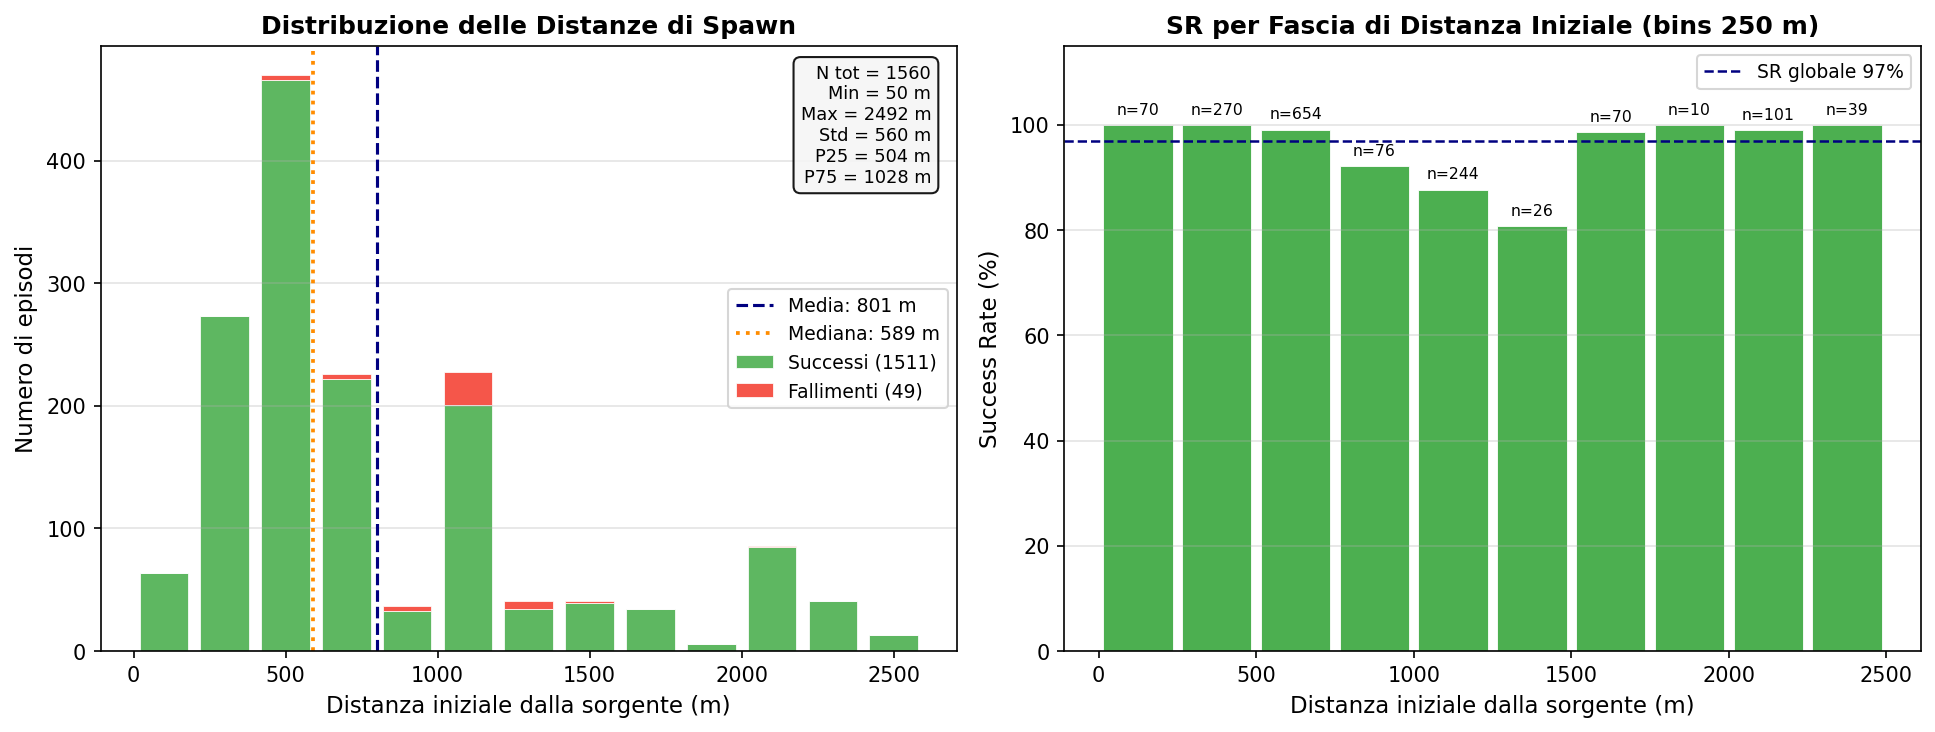
\includegraphics[width=0.82\linewidth]{rl_initial_dist.png}
  \caption{Distribuzione delle distanze iniziali di spawn --- modello \texttt{minimal}.
           La success rate resta elevata su tutte le fasce di distanza iniziale (anche
           oltre 2000\,m), a conferma che la politica generalizza indipendentemente dal
           punto di partenza.}
  \label{fig:rl_initdist}
\end{figure}

\begin{figure}[H]
  \centering
  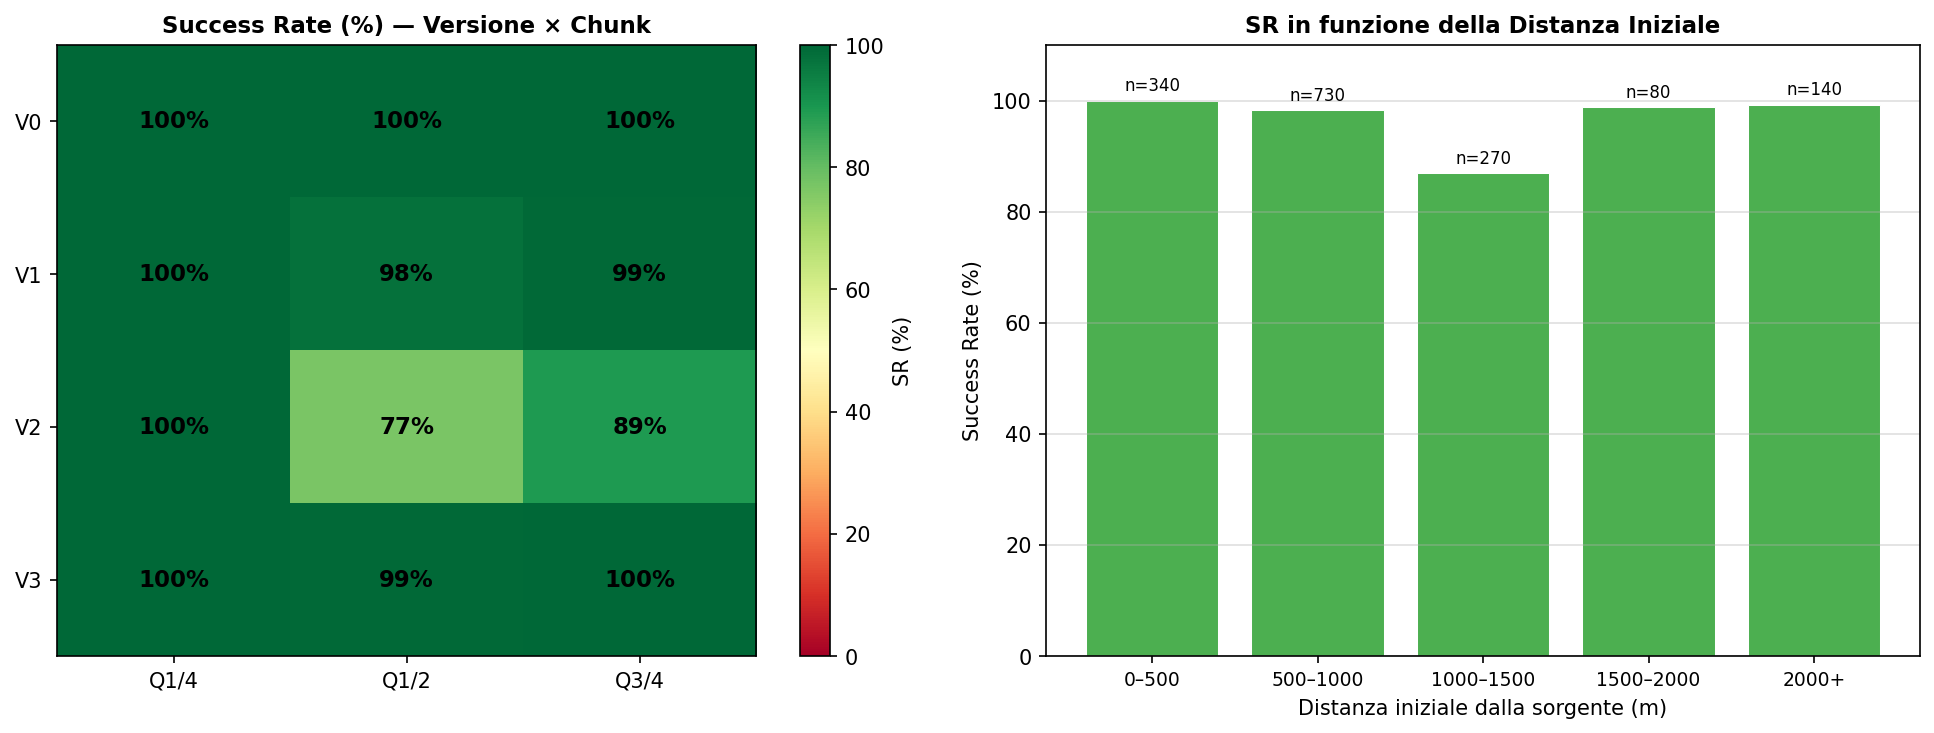
\includegraphics[width=0.82\linewidth]{rl_sr_analysis.png}
  \caption{Success rate per scenario di vento e chunk temporale --- modello
           \texttt{minimal}. Quasi tutte le combinazioni sono risolte vicino al 100\%; le
           uniche difficolt\`a residue --- comunque lievi --- restano su V2 e Q1/2, gli
           stessi scenari critici per l'FCM.}
  \label{fig:rl_sr}
\end{figure}

\begin{figure}[H]
  \centering
  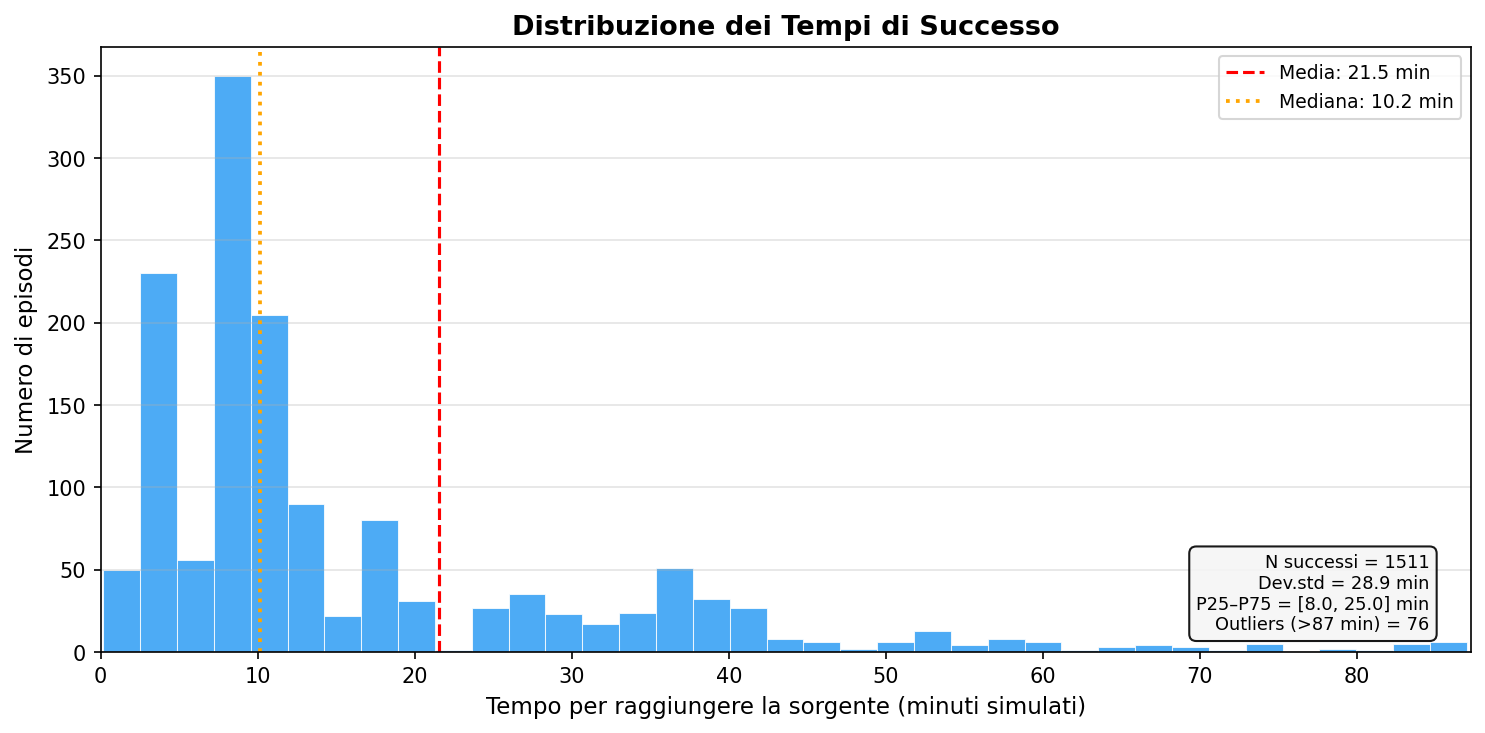
\includegraphics[width=0.82\linewidth]{rl_success_time.png}
  \caption{Distribuzione del tempo al successo --- modello \texttt{minimal}. La gran parte
           degli episodi converge entro pochi minuti simulati, con una coda contenuta:
           l'agente raggiunge la sorgente in modo rapido e consistente.}
  \label{fig:rl_time}
\end{figure}

\begin{figure}[H]
  \centering
  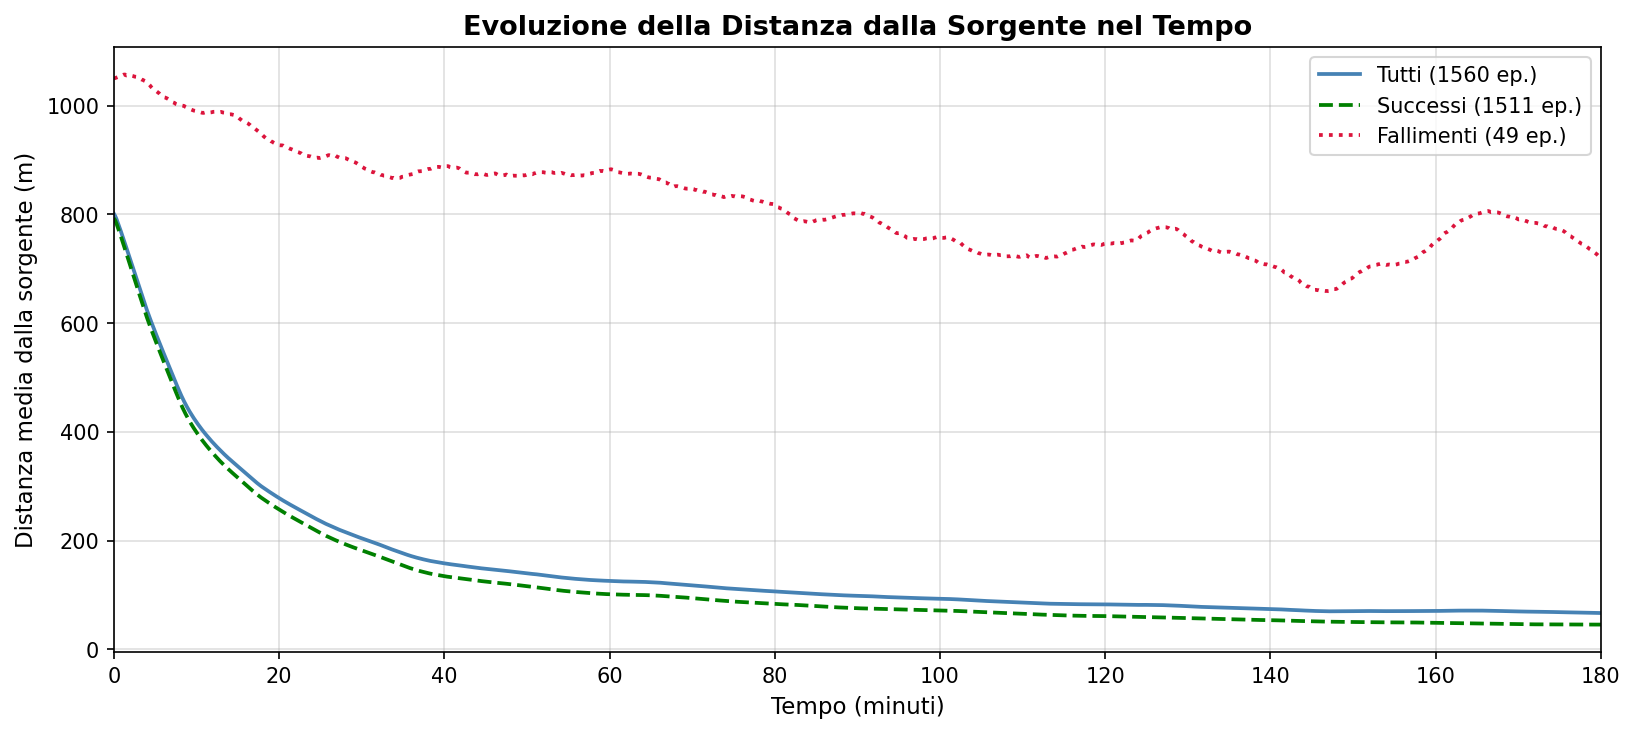
\includegraphics[width=0.82\linewidth]{rl_distance_time.png}
  \caption{Distanza media dalla sorgente nel tempo --- modello \texttt{minimal}. La curva
           dei successi decresce in modo netto e monotono fino all'azzeramento; i rari
           fallimenti restano una frazione marginale, in netto contrasto con i metodi del
           gradiente.}
  \label{fig:rl_dist}
\end{figure}

\subsection{Catena a velocit\`a variabile}
\label{sec:rl_velocity}

Nei modelli visti finora la velocit\`a \`e un parametro fisso del veicolo e l'agente
sceglie solo la direzione. \`E una limitazione: un AUV reale pu\`o modulare la spinta, e
non \`e detto che andare sempre al massimo sia ottimale. Si \`e quindi reso la velocit\`a
una \textbf{scelta dell'agente}.

\paragraph{Spazio d'azione.} Lo spazio d'azione passa da 8 direzioni (passo fisso) a
$\text{Discrete}(8 \times K)$ con $K = 5$: ogni azione codifica \emph{congiuntamente} una
delle 8 direzioni e uno dei 5 livelli di velocit\`a
$\{0{,}2,\,0{,}4,\,\ldots,\,1{,}0\}\cdot v_{\max}$. L'agente sceglie cos\`i a ogni passo
non solo \emph{dove} andare ma anche \emph{quanto} spingere. La velocit\`a ottimale non
\`e imposta da una regola: emerge \textbf{implicitamente} dall'ottimizzazione del ritorno
--- l'agente potrebbe apprendere, ad esempio, che rallentare in prossimit\`a della
sorgente o in controcorrente conviene. La singola azione intera viene decodificata in una
coppia (direzione, velocit\`a) tramite divisione e resto per $K$:

\begin{lstlisting}
def _decode_action(self, action):        # action in {0, ..., 8K-1}
    K = self.config.n_velocity_levels    # K = 5 livelli
    dir_idx = action // K                # una delle 8 direzioni
    vel_idx = action %  K                # livello di velocita'
    velocity = (vel_idx + 1) / K * self.config.max_velocity   # in (0, v_max]
    return dir_idx, velocity             # dove andare + quanto spingere
\end{lstlisting}

\paragraph{Perch\'e una catena di warm-start.} Passare direttamente da un modello a passo
fisso ($1\,\text{m/s}$) a uno con velocit\`a libera fino a $5\,\text{m/s}$ \`e un salto
difficile: lo spazio d'azione si quintuplica (da 8 a 40 azioni) e la dinamica
dell'episodio cambia. L'addestramento \`e perci\`o organizzato a \textbf{catena}, in modo
che ogni incremento sia un piccolo aggiustamento su una policy gi\`a competente anzich\'e
un apprendimento da zero:
\begin{itemize}[leftmargin=1.4em, itemsep=2pt]
    \item il primo stadio ($v_{\max}{=}1$) parte dal modello \texttt{minimal} a passo
          fisso, ne \textbf{trapianta il corpo} (le rappresentazioni gi\`a apprese) ed
          espande la testa d'azione da 8 a 40 uscite; l'agente impara a modulare la
          velocit\`a entro lo stesso tetto di $1\,\text{m/s}$;
    \item ogni stadio successivo ($v_{\max}{=}2,\ldots,5$) riparte dal precedente
          (fine-tuning) e alza progressivamente il tetto di velocit\`a.
\end{itemize}
Ogni stadio \`e valutato su 1560 episodi. Il trapianto della testa d'azione replica i logit
di ciascuna direzione sui $K$ livelli, favorendo all'avvio il livello $v_{\max}$ tramite il
bias (variante \emph{max-bias}), cos\`i che la policy parta equivalente a quella a passo
fisso:

\begin{lstlisting}
# corpo (MLP 256x256) e critico: copiati invariati dal modello minimal.
# testa azione (8 -> 8*K): ogni direzione replicata sui K livelli di velocita'.
for d in range(n_directions):                  # 8 direzioni
    for k in range(K):                         # 5 livelli di velocita'
        row = d * K + k
        W[row] = w_min[d]                      # stessi pesi della direzione d
        B[row] = b_min[d] - (0.0 if k == K-1 else suppress)  # bias sul livello v_max
\end{lstlisting}

\begin{figure}[H]
\centering
\begin{tikzpicture}[
  font=\footnotesize,
  box/.style={draw, rounded corners, minimum height=1.05cm, align=center, inner sep=4pt},
  copied/.style={box, fill=green!14, minimum width=1.7cm},
  body/.style={box, fill=green!14, minimum width=2.7cm},
  changed/.style={box, fill=orange!28, minimum width=1.9cm},
  flow/.style={-{Latex[length=2mm]}, thick},
  map/.style={-{Latex[length=2mm]}, densely dashed, gray}
]
% --- riga Minimal ---
\node[copied] (m0) {obs\\(116)};
\node[body, right=0.7cm of m0] (mb) {corpo MLP\\$256\times256$ (tanh)};
\node[changed, right=0.7cm of mb] (mh) {testa azione\\\textbf{8} (dir.)};
\draw[flow] (m0)--(mb); \draw[flow] (mb)--(mh);
\node[align=right, anchor=east] at ([xshift=-0.25cm]m0.west) {\textbf{minimal}\\passo fisso};
% --- riga v1 ---
\node[copied, below=2.0cm of m0] (v0) {obs\\(116)};
\node[body, right=0.7cm of v0] (vb) {corpo MLP\\$256\times256$ (tanh)};
\node[changed, right=0.7cm of vb] (vh) {testa azione\\\textbf{40} (dir$\times$vel)};
\draw[flow] (v0)--(vb); \draw[flow] (vb)--(vh);
\node[align=right, anchor=east] at ([xshift=-0.25cm]v0.west) {\textbf{v1}\\vel.\ adattiva};
% --- mappature ---
\draw[map] (m0)--(v0) node[midway, fill=white, inner sep=1pt]{copia};
\draw[map] (mb)--(vb) node[midway, fill=white, inner sep=1pt]{copia};
\draw[-{Latex[length=2mm]}, thick, orange!75!black] (mh)--(vh)
   node[midway, fill=white, inner sep=1pt, text=black]{espansione $8\!\to\!40$};
\end{tikzpicture}
\caption{Warm-start del primo stadio (\texttt{minimal} $\to$ v1). Il \textbf{corpo} della
         rete (ingresso a 116 dim.\ e MLP $256\times256$) viene \textbf{copiato} invariato
         (verde); solo la \textbf{testa d'azione} viene \textbf{espansa} da 8 a 40 uscite
         (arancio): ogni direzione viene replicata sui 5 livelli di velocit\`a, con bias
         iniziale verso $v_{\max}$ (all'avvio la policy equivale a quella a passo fisso).}
\label{fig:rl_warmstart_vel}
\end{figure}

\begin{figure}[H]
\centering
\begin{tikzpicture}[
  font=\scriptsize,
  vel/.style={draw, rounded corners, fill=blue!7, minimum width=2.4cm, minimum height=0.52cm, align=center, inner sep=1pt},
  velmax/.style={draw, rounded corners, fill=orange!30, minimum width=2.4cm, minimum height=0.52cm, align=center, inner sep=1pt},
  dir/.style={draw, rounded corners, fill=green!16, minimum width=2.3cm, minimum height=0.95cm, align=center},
  a/.style={-{Latex[length=1.5mm]}, gray}
]
\node[dir] (d) {direzione $d_i$\\(1 delle 8)};
\node[vel, right=1.9cm of d] (v3) {$(d_i,\;0{,}6\,v_{\max})$};
\node[vel, above=0.1cm of v3] (v2) {$(d_i,\;0{,}4\,v_{\max})$};
\node[vel, above=0.1cm of v2] (v1) {$(d_i,\;0{,}2\,v_{\max})$};
\node[vel, below=0.1cm of v3] (v4) {$(d_i,\;0{,}8\,v_{\max})$};
\node[velmax, below=0.1cm of v4] (v5) {$(d_i,\;v_{\max})$};
\foreach \n in {v1,v2,v3,v4,v5} \draw[a] (d.east)--(\n.west);
\node[anchor=west, align=left, text width=3.5cm] at ([xshift=0.5cm]v3.east)
  {peso della direzione \textbf{replicato} sui 5 livelli; il livello $v_{\max}$ (arancio)
   riceve il \textbf{bias} iniziale};
\node[below=0.7cm of d.south, anchor=north, align=center, text width=3.3cm]
  {ripetuto per le \textbf{8 direzioni}\\$\Rightarrow\; 8\times5 = \mathbf{40}$ uscite};
\end{tikzpicture}
\caption{Focus sulla testa d'azione (espansione $8\to40$). Ciascuna delle 8 direzioni
         della testa \texttt{minimal} viene sdoppiata nei 5 livelli di velocit\`a
         $(d_i, v_k)$: i pesi sono replicati e il livello $v_{\max}$ \`e favorito
         all'avvio, cos\`i la policy parte equivalente a quella a passo fisso.}
\label{fig:rl_testa_azione}
\end{figure}

\begin{table}[H]
\centering
\renewcommand{\arraystretch}{1.6}
\setlength{\tabcolsep}{3pt}
\small
\begin{tabular}{C{1.4cm} C{1.0cm} C{2.2cm} C{1.15cm} C{1.15cm} C{1.15cm} C{1.15cm} C{1.15cm} C{1.15cm} C{1.15cm}}
\toprule
\rowcolor{headerbg}
\textcolor{white}{\textbf{$v_{\max}$}} &
\textcolor{white}{\textbf{SR\%}} &
\textcolor{white}{\textbf{Step (min)}} &
\textcolor{white}{\textbf{V0}} &
\textcolor{white}{\textbf{V1}} &
\textcolor{white}{\textbf{V2}} &
\textcolor{white}{\textbf{V3}} &
\textcolor{white}{\textbf{Q1/4}} &
\textcolor{white}{\textbf{Q1/2}} &
\textcolor{white}{\textbf{Q3/4}} \\
\midrule
1\,m/s & 97{,}1 & 119{,}6 (19{,}9) & 99{,}5 & 100{,}0 & 89{,}7 & 99{,}2 & 100{,}0 & 95{,}0 & 96{,}3 \\
\rowcolor{rowalt}
2\,m/s & 99{,}7 & 69{,}5 (11{,}6) & 100{,}0 & 99{,}5 & 99{,}2 & 100{,}0 & 100{,}0 & 99{,}0 & 100{,}0 \\
3\,m/s & 99{,}9 & 46{,}9 (7{,}8) & 100{,}0 & 100{,}0 & 99{,}7 & 100{,}0 & 100{,}0 & 99{,}8 & 100{,}0 \\
\rowcolor{rowalt}
4\,m/s & 99{,}9 & 38{,}2 (6{,}4) & 100{,}0 & 100{,}0 & 99{,}5 & 100{,}0 & 100{,}0 & 100{,}0 & 99{,}6 \\
\rowcolor{best}
\textbf{5\,m/s} & \textbf{99{,}9} & \textbf{27{,}8 (4{,}6)} & 100{,}0 & 100{,}0 & \textbf{99{,}7} & 100{,}0 & 100{,}0 & 100{,}0 & 99{,}8 \\
\bottomrule
\end{tabular}
\caption{Catena PPO a velocit\`a variabile (1560 episodi per stadio, $K{=}5$).
         ``Step (min)'' riporta gli step medi al successo e, tra parentesi, i minuti
         corrispondenti ($1\,\text{step}=10\,\text{s}$). All'aumentare di $v_{\max}$
         crescono SR e velocit\`a (step medi da $\sim$20 a $\sim$5\,min).}
\label{tab:rl_velocity}
\end{table}

Gi\`a il primo stadio ($v_{\max}{=}1$, equivalente in velocit\`a al modello a passo
fisso) raggiunge il $97{,}1\%$, superando il $96{,}9\%$ di \texttt{minimal}: rendere la
velocit\`a una scelta non costa nulla nemmeno a parit\`a di tetto. Alzare $v_{\max}$
produce due benefici congiunti: l'SR sale al $99{,}7$--$99{,}9\%$ e gli step medi al
successo crollano da 120 a 28 (oltre $4\times$ pi\`u veloce). Il guadagno maggiore \`e su
\textbf{V2}, lo scenario a corrente forte: la velocit\`a netta dell'agente \`e
$v_{\text{agente}} - v_{\text{corrente}}$, e con pi\`u velocit\`a disponibile l'agente
batte pi\`u facilmente la corrente contraria, passando da $89{,}7\%$ a $99{,}7\%$. A
partire da $v_{\max}{=}3$ le prestazioni sono sostanzialmente sature ($\approx 99{,}9\%$):
l'ulteriore margine di velocit\`a serve solo a ridurre il tempo al successo, non
l'affidabilit\`a.

\paragraph{Andamento della velocit\`a media.} In media l'agente resta prossimo a
$v_{\max}$ a ogni stadio; la modulazione (gli avvallamenti della media e l'ampiezza della
banda) \textbf{non \`e monot\`ona} in $v_{\max}$: \`e \textbf{massima agli stadi
intermedi} ($v_{\max}{=}2,3$) e \textbf{quasi assente agli estremi}. A $v_{\max}{=}1$ il
passo pieno ($10\,\text{m}$) \`e molto minore del raggio di successo ($50\,\text{m}$): non
c'\`e rischio di scavalcare la sorgente, andare al massimo \`e quasi sempre sicuro e la
media resta piatta. A $v_{\max}{=}5$ il passo pieno ($50\,\text{m}$) eguaglia il raggio e,
grazie alla cattura sul segmento percorso, una falcata piena centra comunque il bersaglio:
di nuovo conviene il massimo. Ai valori intermedi, invece, il passo diventa confrontabile
con la scala di avvicinamento e i rallentamenti correttivi si fanno pi\`u evidenti.

\begin{figure}[H]
  \centering
  \begin{subfigure}{0.62\linewidth}
    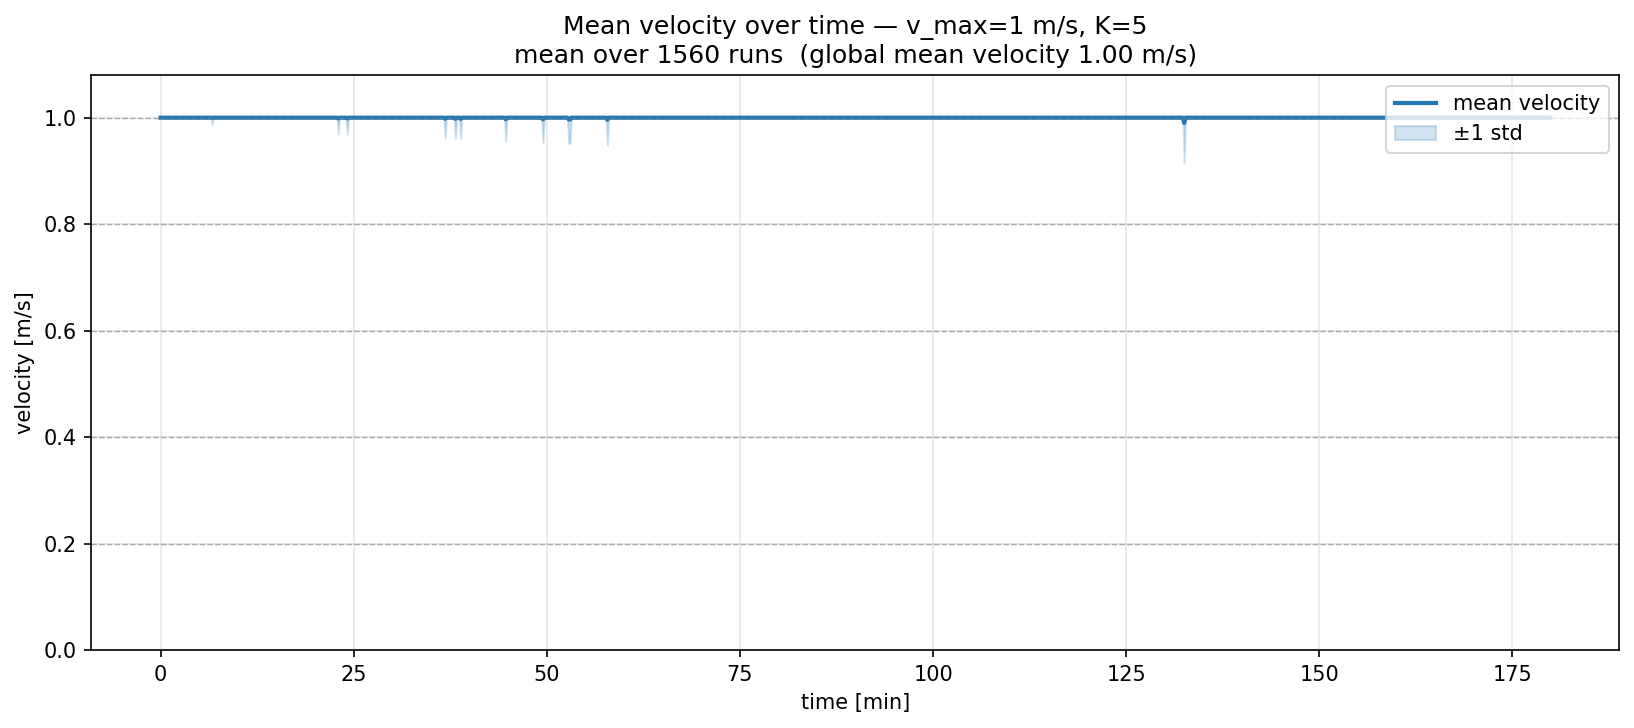
\includegraphics[width=\linewidth]{velocity_mean_over_time_v1.png}
    \caption{$v_{\max}{=}1\,\text{m/s}$}
  \end{subfigure}

  \vspace{6pt}
  \begin{subfigure}{0.62\linewidth}
    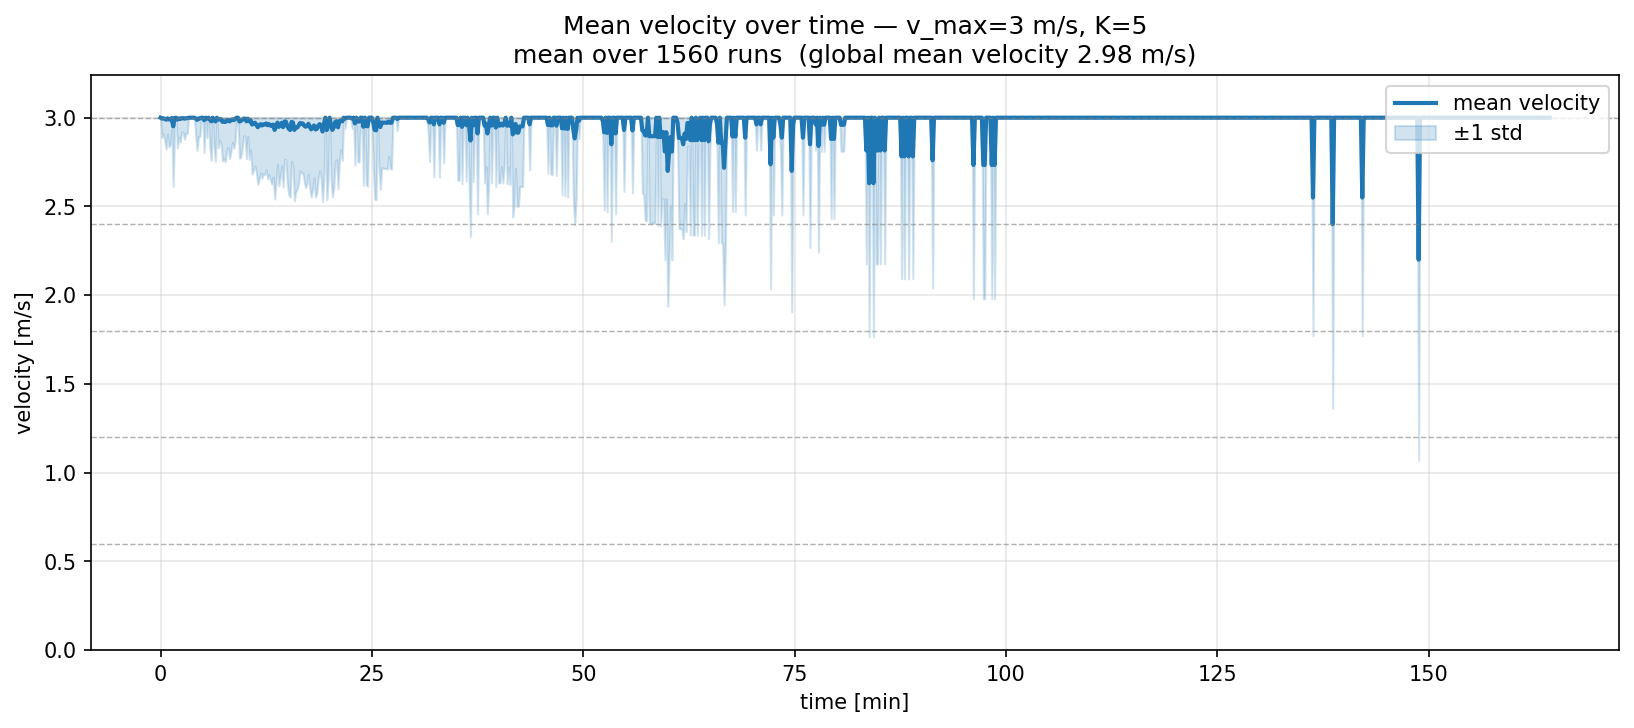
\includegraphics[width=\linewidth]{velocity_mean_over_time_v3.png}
    \caption{$v_{\max}{=}3\,\text{m/s}$}
  \end{subfigure}

  \vspace{6pt}
  \begin{subfigure}{0.62\linewidth}
    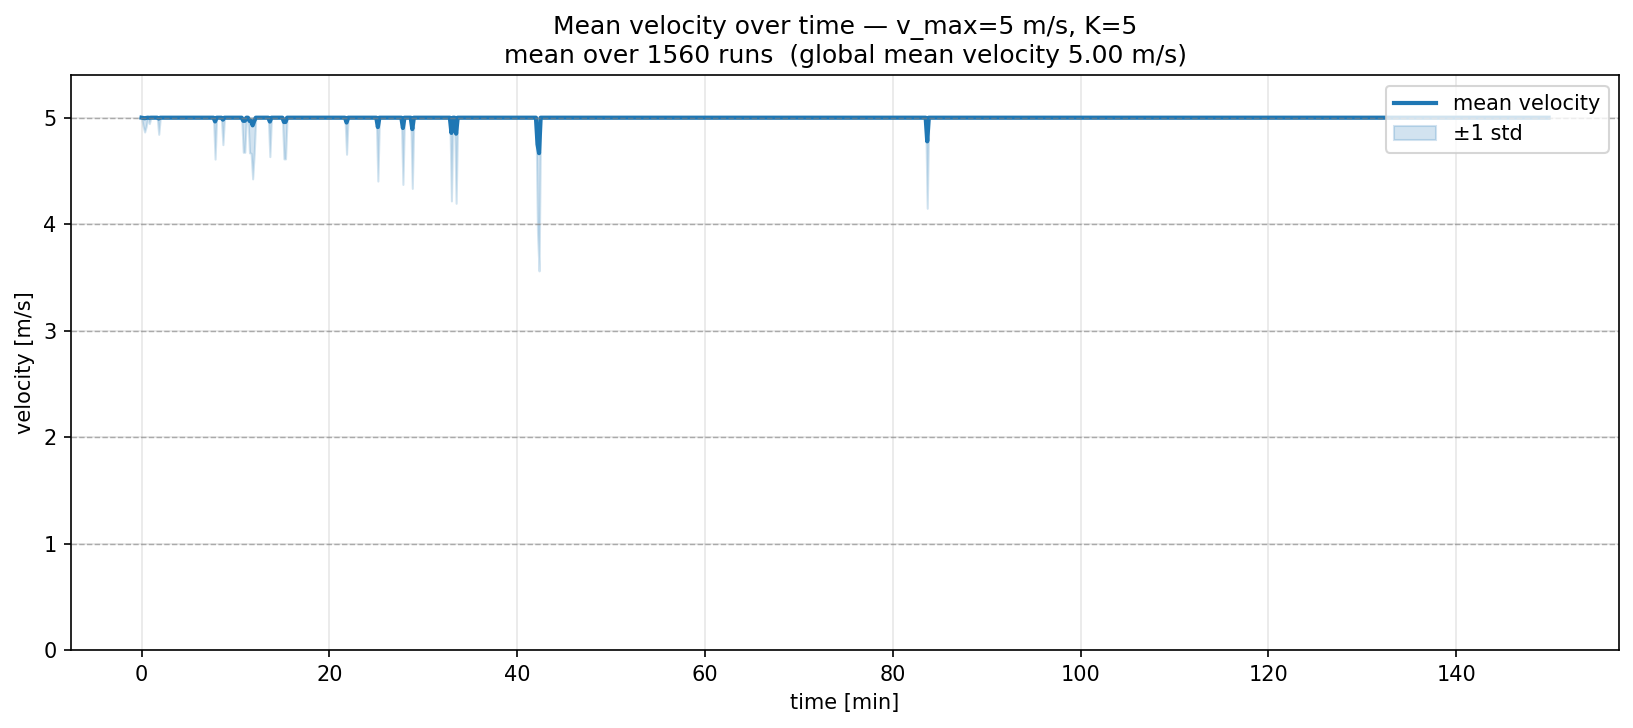
\includegraphics[width=\linewidth]{velocity_mean_over_time_v5.png}
    \caption{$v_{\max}{=}5\,\text{m/s}$}
  \end{subfigure}
  \caption{PPO adattivo: velocit\`a media (su tutte le run) nel tempo, stadi
           $v_{\max}{=}1{,}3{,}5$. In media l'agente resta prossimo a $v_{\max}$ ma modula
           il passo con rallentamenti correttivi, pi\`u evidenti allo stadio intermedio e
           quasi assenti agli estremi.}
  \label{fig:rl_velocity_time}
\end{figure}

\subsection{Formazione a singola vs.\ doppia corona}
\label{sec:rl_dual}

La doppia corona (Tabella~\ref{tab:obs}) aggiunge alla corona locale a
$r_s = 20\,\text{m}$ una \textbf{seconda corona} di 8 slave a $r_{s2} = 50\,\text{m}$, per
dare al master informazione sul plume a scala spaziale pi\`u larga. La domanda \`e:
questa seconda corona \textbf{serve}, e \textbf{a quali velocit\`a}?

\paragraph{Un primo confronto, e perch\'e \`e viziato.} Il primo tentativo ha addestrato
il modello a doppia corona \emph{da zero}, con la stessa configurazione del riferimento
\texttt{minimal} (Tabella~\ref{tab:dualring}).

\begin{table}[H]
\centering
\renewcommand{\arraystretch}{1.3}
\small
\begin{tabular}{L{4.2cm} C{3.3cm} C{3.3cm}}
\toprule
\rowcolor{headerbg}
\textcolor{white}{\textbf{Metrica}} &
\textcolor{white}{\textbf{Singola corona (116)}} &
\textcolor{white}{\textbf{Doppia corona (196)}} \\
\midrule
\rowcolor{rowalt}
SR globale & \textbf{96{,}9\%} & 93{,}0\% \\
Step medi (succ.) & 129{,}2 & \textbf{114{,}4} \\
\midrule
V1 & \textbf{99{,}0\%} & 90{,}3\% \\
\rowcolor{rowalt}
V2 & \textbf{88{,}7\%} & 82{,}3\% \\
Q1/2 & \textbf{93{,}5\%} & 86{,}2\% \\
\bottomrule
\end{tabular}
\caption{Primo confronto fra singola corona (\texttt{minimal}, $r_s{=}20\,\text{m}$) e
         doppia corona ($20\,\text{m}$ + $50\,\text{m}$), entrambe a passo fisso e
         addestrate \textbf{da zero}. Il confronto \`e viziato: cambia insieme il sensore e
         la difficolt\`a di ottimizzare da zero una rete pi\`u grande. La
         Tabella~\ref{tab:dual_vmax} lo rif\`a in modo controllato.}
\label{tab:dualring}
\end{table}

Letto cos\`i, il risultato sembrerebbe chiudere la questione: la doppia corona
\emph{non} supera il riferimento, con un calo di $3{,}9$ punti concentrato su V1, V2 e
Q1/2. Il confronto \`e per\`o \textbf{viziato}, perch\'e cambia due cose insieme: il
sensore \emph{e} la dimensione della rete da ottimizzare da zero. Una rete con 80 ingressi
in pi\`u \`e pi\`u difficile da addestrare a partire da pesi casuali, e il calo osservato
confonde l'effetto dell'informazione con quello dell'ottimizzazione. Non si pu\`o quindi
concludere che la seconda corona sia dannosa: si pu\`o solo dire che addestrare da zero
una rete pi\`u grande rende meno.

\paragraph{Un protocollo equo: warm-start.} Per isolare il \emph{solo} effetto del
sensore, la doppia corona \`e ottenuta per \textbf{warm-start dal corrispondente modello a
singola corona}: per ogni $v_{\max} \in \{1,\ldots,5\}$ il modello a doppia corona parte
da quello a singola corona di pari velocit\`a, allargando lo strato di ingresso da 116 a
196 dimensioni e \textbf{azzerando} le colonne della corona-2. All'avvio la rete \`e
quindi \emph{identica} alla singola corona --- ignora la corona-2 --- e impara durante il
fine-tuning se e come usarla. Ogni eventuale differenza \`e cos\`i attribuibile al solo
sensore, non al protocollo. Ogni modello \`e valutato su 1560 episodi. L'allargamento dello
strato d'ingresso conserva le colonne condivise e azzera quelle della corona-2:

\begin{lstlisting}
# doppia corona (196) warm-startata dalla singola (116):
# tutti i pesi copiati dal single; nello strato d'ingresso le colonne condivise
# sono rimappate e le 80 colonne della corona-2 sono AZZERATE.
W_in_dual[:, shared_cols] = W_in_single    # resto identico al single
W_in_dual[:, ring2_cols]  = 0.0            # corona-2 non contribuisce all'avvio
# le statistiche di VecNormalize della corona-2 restano neutre (media 0, var 1).
\end{lstlisting}

\begin{figure}[H]
\centering
\begin{tikzpicture}[
  font=\footnotesize,
  box/.style={draw, rounded corners, minimum height=1.05cm, align=center, inner sep=4pt},
  copied/.style={box, fill=green!14},
  body/.style={box, fill=green!14, minimum width=2.7cm},
  head/.style={box, fill=green!14, minimum width=1.9cm},
  changed/.style={box, fill=orange!28},
  flow/.style={-{Latex[length=2mm]}, thick},
  map/.style={-{Latex[length=2mm]}, densely dashed, gray}
]
% --- riga v1 (singola corona) ---
\node[copied, minimum width=1.9cm] (s0) {obs single\\(116)};
\node[body, right=0.7cm of s0] (sb) {corpo MLP\\$256\times256$ (tanh)};
\node[head, right=0.7cm of sb] (sh) {testa azione\\\textbf{40}};
\draw[flow] (s0)--(sb); \draw[flow] (sb)--(sh);
\node[align=right, anchor=east] at ([xshift=-0.25cm]s0.west) {\textbf{v1}\\singola corona};
% --- riga doppia corona: ingresso segmentato 116 + 80 ---
\node[copied, below=2.0cm of s0, minimum width=1.15cm] (d0a) {116};
\node[changed, right=0pt of d0a, minimum width=1.15cm] (d0b) {+80\\corona-2\\(=0)};
\node[body, right=0.7cm of d0b] (db) {corpo MLP\\$256\times256$ (tanh)};
\node[head, right=0.7cm of db] (dh) {testa azione\\\textbf{40}};
\draw[flow] (d0b)--(db); \draw[flow] (db)--(dh);
\node[align=right, anchor=east] at ([xshift=-0.25cm]d0a.west) {\textbf{doppia}\\corona (196)};
% --- mappature ---
\draw[-{Latex[length=2mm]}, thick, orange!75!black] (s0.south)--(d0a.north)
   node[midway, xshift=1.5cm, fill=white, inner sep=1.5pt, text=black]{ingresso $116\!\to\!196$};
\draw[map] (sb)--(db) node[midway, fill=white, inner sep=1pt]{copia};
\draw[map] (sh)--(dh) node[midway, fill=white, inner sep=1pt]{copia};
\end{tikzpicture}
\caption{Warm-start della doppia corona (esempio a $v_{\max}{=}1$; a ogni livello \`e
         analogo, dal rispettivo modello a singola corona). \textbf{Corpo} e \textbf{testa
         d'azione} sono \textbf{copiati} invariati (verde); si allarga solo lo
         \textbf{strato d'ingresso} da 116 a 196 (arancio), aggiungendo 80 colonne per la
         corona-2 con \textbf{pesi inizializzati a zero}. All'avvio la rete \`e identica a
         v1 e ignora la corona-2; il fine-tuning decide se e come usarla.}
\label{fig:rl_warmstart_dual}
\end{figure}

\begin{table}[H]
\centering
\renewcommand{\arraystretch}{1.3}
\small
\begin{tabular}{C{1.3cm} C{1.5cm} C{1.5cm} C{2.6cm} C{2.6cm} C{1.7cm}}
\toprule
\rowcolor{headerbg}
\textcolor{white}{\textbf{$v_{\max}$}} &
\textcolor{white}{\textbf{SR sing.}} &
\textcolor{white}{\textbf{SR dopp.}} &
\textcolor{white}{\textbf{Step sing.}} &
\textcolor{white}{\textbf{Step dopp.}} &
\textcolor{white}{\textbf{$\Delta$step}} \\
\midrule
1 & 97{,}1\% & 95{,}8\% & 119{,}6 (19{,}9\,min) & 97{,}8 (16{,}3\,min) & \textcolor{green!50!black}{\textbf{$-$18{,}2\%}} \\
\rowcolor{rowalt}
2 & 99{,}7\% & 99{,}7\% & 69{,}5 (11{,}6\,min) & 49{,}8 (8{,}3\,min) & \textcolor{green!50!black}{\textbf{$-$28{,}3\%}} \\
3 & 99{,}9\% & \textbf{100{,}0\%} & 46{,}9 (7{,}8\,min) & 31{,}3 (5{,}2\,min) & \textcolor{green!50!black}{\textbf{$-$33{,}2\%}} \\
\rowcolor{rowalt}
4 & 99{,}9\% & 99{,}9\% & 38{,}2 (6{,}4\,min) & 25{,}3 (4{,}2\,min) & \textcolor{green!50!black}{\textbf{$-$33{,}6\%}} \\
5 & 99{,}9\% & \textbf{100{,}0\%} & 27{,}8 (4{,}6\,min) & 20{,}9 (3{,}5\,min) & \textcolor{green!50!black}{\textbf{$-$24{,}8\%}} \\
\bottomrule
\end{tabular}
\caption{Singola vs.\ doppia corona a ogni $v_{\max}$ (ogni doppia corona warm-startata
         dal modello a singola corona omologo; 1560 episodi per cella). ``Step'' = step
         medi al successo (minuti tra parentesi). $\Delta$step = variazione relativa dei
         passi (verde = doppia pi\`u veloce).}
\label{tab:dual_vmax}
\end{table}

Il quadro \textbf{si ribalta} rispetto alla lettura precedente, e per due motivi distinti.
Primo, \textbf{il costo di SR \`e confinato a $v_{\max}{=}1$}: gi\`a con il solo
warm-start la penalit\`a scende da $-3{,}9$ a $-1{,}3$ --- prova che gran parte del calo
originale era difficolt\`a di ottimizzazione, non informazione dannosa --- e ai livelli
superiori non si ripresenta affatto: a v2--v5 l'SR della doppia corona \`e \emph{pari o
superiore} a quello della singola. Secondo, \textbf{il guadagno di step non si assottiglia
ma cresce}: da $-18\%$ (v1) sale a un picco di $\sim -34\%$ (v3--v4), per poi ridursi a
$-25\%$ a v5 per effetto pavimento (la singola \`e gi\`a a $\sim 28$ step, vicino al
minimo geometrico).

\paragraph{Sguardo ravvicinato a $v_{\max}{=}1$.} A $v_{\max}{=}1$ --- l'unico livello con
un costo di SR --- il residuo $-1{,}3$ \`e concentrato in \textbf{V2}
($89{,}7 \to 86{,}2$) e \textbf{Q3/4} ($96{,}3 \to 90{,}4$), mentre su Q1/2 la doppia
corona \`e in vantaggio ($+2{,}1$). Appaiando i 1560 episodi per (sorgente, vento, chunk,
episodio) si isolano i casi in cui le due configurazioni divergono
(Tabella~\ref{tab:dual_paired}).

\begin{table}[H]
\centering
\renewcommand{\arraystretch}{1.3}
\small
\begin{tabular}{L{6.5cm} C{3.0cm}}
\toprule
\rowcolor{headerbg}
\textcolor{white}{\textbf{Esito appaiato}} &
\textcolor{white}{\textbf{N. episodi}} \\
\midrule
\rowcolor{rowalt}
Entrambi successo                       & 1463 \\
Entrambi fallimento                     & 13 \\
\rowcolor{worst}
Singola OK, \textbf{doppia FALLISCE}    & \textbf{52} \\
Singola fallisce, doppia OK             & 32 \\
\midrule
\textbf{Netto}                          & \textbf{$-20$ ($=-1{,}3\%$)} \\
\bottomrule
\end{tabular}
\caption{Matrice degli esiti appaiati singola vs.\ doppia corona a $v_{\max}{=}1$.}
\label{tab:dual_paired}
\end{table}

I 52 fallimenti differenziali hanno una firma nettissima (Figura~\ref{fig:dual_v2}): sono \textbf{tutti
\texttt{timeout}} (nessuna uscita dal dominio), l'$81\%$ \`e su \textbf{vento V2} (42/52)
nei chunk a corrente sostenuta, avvengono su \textbf{spawn lontani} (distanza iniziale
media $1070\,\text{m}$ contro $690\,\text{m}$ della media generale) e \textbf{non sono
near-miss}: $36/52$ non scendono mai sotto $150\,\text{m}$ dalla sorgente (distanza minima
mediana $322\,\text{m}$). L'agente, in altre parole, \textbf{si perde}; non ``non riesce a
frenare''. Il crollo \`e tutto nel regime ``lontano $+$ corrente forte'': in V2 la SR per
fascia di distanza iniziale passa da $+1{,}1$ (300--700\,m) a $-15{,}2$ (1100--1600\,m)
fino a $-83{,}3$ (oltre 1600\,m).

\begin{figure}[H]
  \centering
  \begin{subfigure}{0.49\linewidth}
    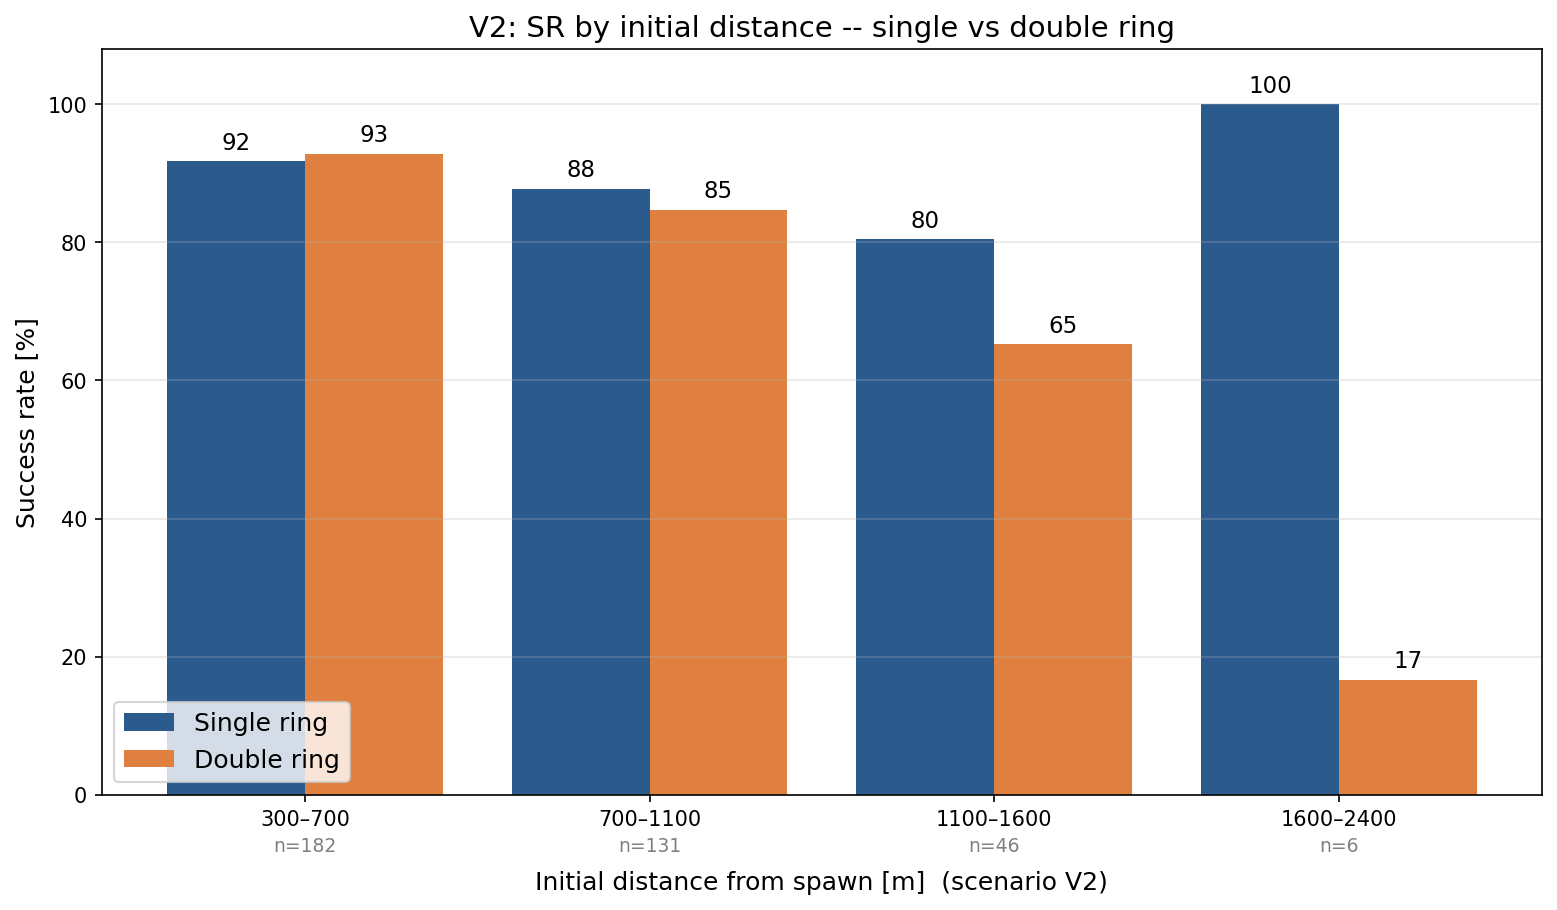
\includegraphics[width=\linewidth]{sr_vs_initdist_V2.png}
    \caption{SR per fascia di distanza iniziale (V2).}
  \end{subfigure}
  \hfill
  \begin{subfigure}{0.49\linewidth}
    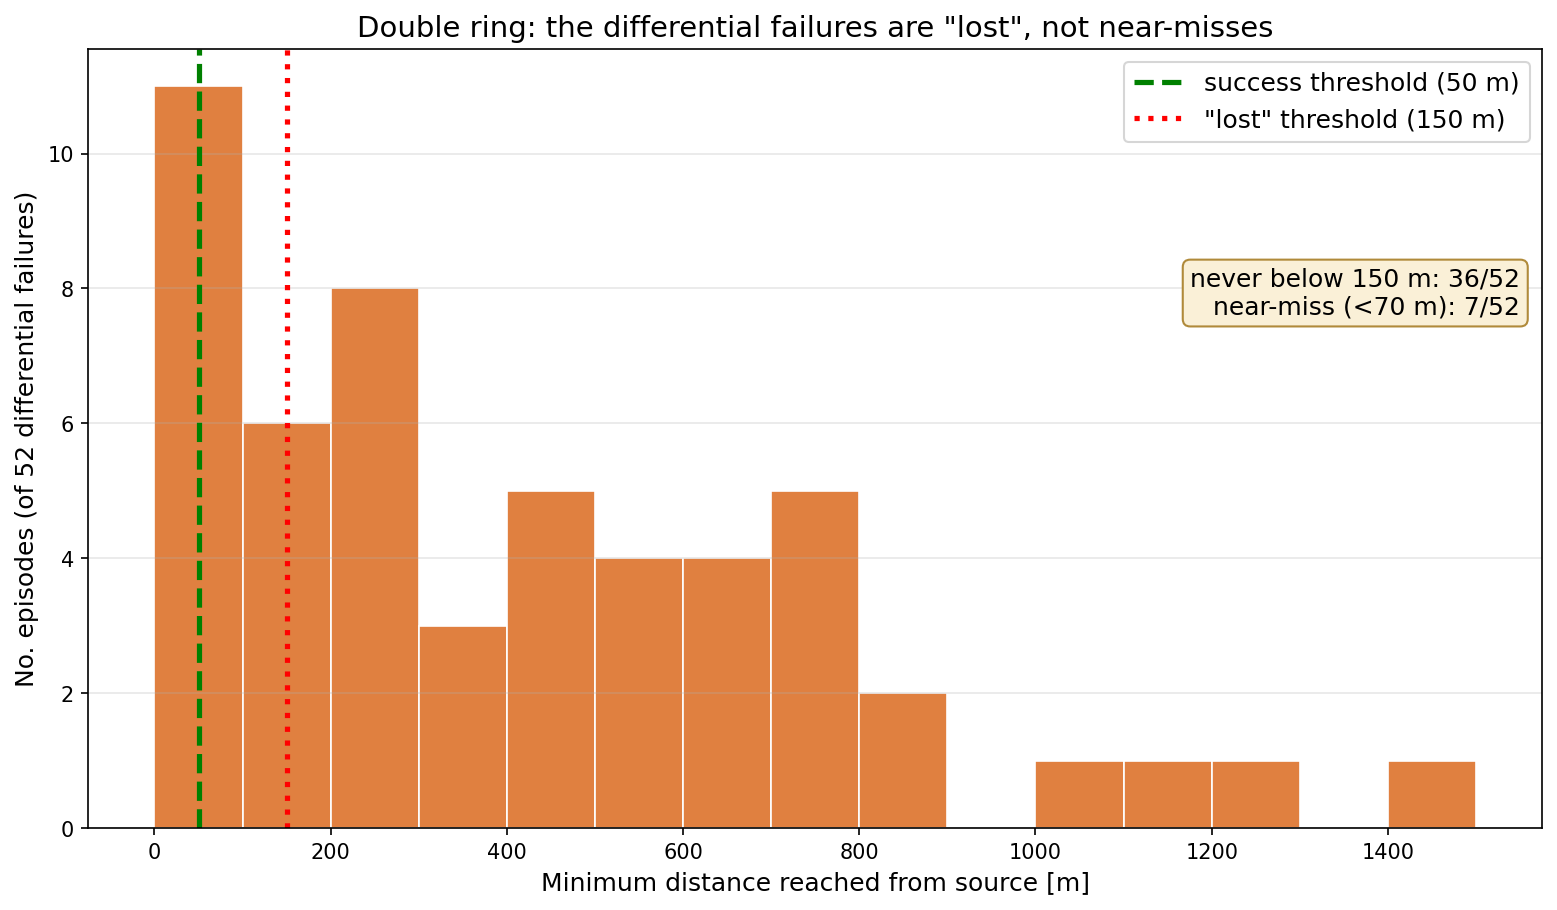
\includegraphics[width=\linewidth]{diff_fail_mindist.png}
    \caption{Distanza minima nei fallimenti differenziali.}
  \end{subfigure}
  \caption{Firma del costo di affidabilit\`a della doppia corona a $v_{\max}{=}1$ nello
           scenario V2. A sinistra: sugli spawn vicini la doppia corona \`e pari o migliore,
           ma sulle fasce lontane ($>$1100\,m) la SR crolla rispetto alla singola. A destra:
           i fallimenti differenziali non sono \emph{near-miss} --- la distanza minima dalla
           sorgente resta elevata, l'agente ``si perde'' anzich\'e non riuscire a frenare.}
  \label{fig:dual_v2}
\end{figure}

Vanno per\`o letti anche i \textbf{32 casi opposti}, in cui la singola fallisce e la
doppia riesce. Anch'essi sono tutti timeout della singola e concentrati in V2 (28/32), ma
con firma \emph{complementare}: il chunk dominante \`e \textbf{Q1/2} (25/32) anzich\'e
Q3/4, e gli spawn sono a distanza \textbf{moderata} (media $749\,\text{m}$ contro
$1070\,\text{m}$). La doppia corona non \`e dunque uniformemente peggiore:
\textbf{redistribuisce} i successi. Sui chunk Q1/2 il segnale a 50\,m aiuta a tenere la
rotta ed \`e in attivo (25 recuperi contro 14 perdite); su Q3/4, con spawn pi\`u lontani e
corrente pi\`u sostenuta, lo stesso segnale inganna ed \`e in passivo (7 recuperi contro
38 perdite). Il bilancio netto, $-20$ episodi, \`e uno \textbf{spostamento della frontiera
di successo}, non una regressione generalizzata.

\paragraph{Interpretazione.} Il filo che tiene insieme tutti i risultati \`e uno solo: la
corona-2 sente il campo \textbf{pi\`u lontano} ($50\,\text{m}$), e il valore di questa
``vista lontana'' dipende da \emph{quanto lontano l'agente sta per muoversi}, cio\`e dalla
lunghezza del passo. A $v_{\max}$ alto le falcate sono grandi (fino a $50\,\text{m}$) e
una falcata mal puntata scavalca la rotta, costando correzioni; la corona-2, vedendo
esattamente ``un passo avanti'', permette di puntarle bene ed evita gli \emph{overshoot}
che rallentano la singola --- da cui il guadagno crescente con $v_{\max}$. Il costo di
affidabilit\`a a $v_{\max}{=}1$ \`e lo stesso meccanismo ribaltato: a passi piccoli
l'agente resta pi\`u a lungo immerso nel campo e in V2, con plume fortemente avvettato, il
segnale a 50\,m pu\`o puntare \emph{lungo la corrente} anzich\'e verso la sorgente; sugli
spawn lontani l'agente si fida del segnale distante, sbaglia direzione e va in timeout.
Alle velocit\`a superiori attraversa quel regime troppo in fretta perch\'e l'errore si
accumuli, e il costo sparisce.

Vale infine la pena chiedersi perch\'e l'agente non \emph{ignori} semplicemente la
corona-2 quando non conviene. Ignorarla equivarrebbe a pesi d'ingresso esattamente nulli,
una soluzione che la discesa del gradiente non raggiunge: anche partendo da zero, come nel
warm-start, i gradienti spostano quei pesi. Soprattutto, usarla \emph{aumenta} il reward
--- lo \texttt{step\_penalty} premia l'arrivare prima e la corona-2 d\`a traiettorie pi\`u
dirette --- quindi l'ottimizzatore \textbf{sceglie} di usarla. In sintesi: la seconda
corona \`e un \textbf{vantaggio netto a partire da $v_{\max}{=}2$} (stessa affidabilit\`a,
$25$--$34\%$ di passi in meno), e solo a $v_{\max}{=}1$ si osserva un piccolo scambio
robustezza/velocit\`a. La conclusione del primo confronto --- ``per questo dominio la
singola corona \`e sufficiente'' --- era un artefatto dell'aver addestrato da zero e
dell'aver guardato un solo livello di velocit\`a.

\subsection{Test di modulazione: raggio di successo a 10\,m}
\label{sec:rl_r10}

I risultati della catena a velocit\`a variabile mostrano che, in media, l'agente resta
prossimo a $v_{\max}$. Sorge quindi una domanda: l'agente \emph{sa} davvero rallentare, o
gli conviene sempre andare al massimo? Con un raggio di successo di $50\,\text{m}$ la
domanda \`e mal posta, perch\'e il raggio \`e grande quanto un passo pieno
($50\,\text{m}$ a $v_{\max}{=}5$): l'agente pu\`o \textbf{piombare} sulla sorgente a piena
velocit\`a e centrare comunque il bersaglio, senza alcun bisogno di rallentare.

Per rendere il compito pi\`u stringente si \textbf{restringe il raggio di successo a
$10\,\text{m}$}. Ora un passo pieno da $50\,\text{m}$ \textbf{scavalca} un bersaglio da
$10\,\text{m}$, e centrarlo non \`e pi\`u banale: per riuscirci l'agente impara a
\emph{rallentare} in avvicinamento, oppure adotta un'altra strategia? Il modello \`e
ottenuto per fine-tuning a partire dallo stadio $v_{\max}{=}5$, cambiando \emph{solo} il
raggio di successo ($50 \to 10\,\text{m}$), con soglia di stagnazione ridotta,
$lr = 10^{-4}$ e curriculum $\alpha = 0{,}8$, per $2$\,M timestep; la valutazione \`e su
1560 episodi, identica agli altri stadi.

\begin{table}[H]
\centering
\renewcommand{\arraystretch}{1.6}
\setlength{\tabcolsep}{2pt}
\small
\begin{tabular}{C{2.4cm} C{1.0cm} C{2.1cm} C{1.1cm} C{1.1cm} C{1.1cm} C{1.1cm} C{1.1cm} C{1.1cm} C{1.1cm}}
\toprule
\rowcolor{headerbg}
\textcolor{white}{\textbf{Raggio}} &
\textcolor{white}{\textbf{SR\%}} &
\textcolor{white}{\textbf{Step (min)}} &
\textcolor{white}{\textbf{V0}} &
\textcolor{white}{\textbf{V1}} &
\textcolor{white}{\textbf{V2}} &
\textcolor{white}{\textbf{V3}} &
\textcolor{white}{\textbf{Q1/4}} &
\textcolor{white}{\textbf{Q1/2}} &
\textcolor{white}{\textbf{Q3/4}} \\
\midrule
$v_{\max}{=}5$, 50\,m & 99{,}9 & 27{,}8 (4{,}6) & 100{,}0 & 100{,}0 & 99{,}7 & 100{,}0 & 100{,}0 & 100{,}0 & 99{,}8 \\
\rowcolor{rowalt}
$v_{\max}{=}5$, 10\,m &
  \shortstack{99{,}2\\[-1pt]{\scriptsize\textcolor{red!60!black}{$-$0{,}7}}} &
  \shortstack{54{,}8 (9{,}1)\\[-1pt]{\scriptsize\textcolor{gray!35!black}{$+$27{,}0}}} &
  \shortstack{100{,}0\\[-1pt]{\scriptsize 0{,}0}} &
  \shortstack{98{,}5\\[-1pt]{\scriptsize\textcolor{red!60!black}{$-$1{,}5}}} &
  \shortstack{98{,}5\\[-1pt]{\scriptsize\textcolor{red!60!black}{$-$1{,}2}}} &
  \shortstack{100{,}0\\[-1pt]{\scriptsize 0{,}0}} &
  \shortstack{98{,}7\\[-1pt]{\scriptsize\textcolor{red!60!black}{$-$1{,}3}}} &
  \shortstack{99{,}4\\[-1pt]{\scriptsize\textcolor{red!60!black}{$-$0{,}6}}} &
  \shortstack{99{,}6\\[-1pt]{\scriptsize\textcolor{red!60!black}{$-$0{,}2}}} \\
\bottomrule
\end{tabular}
\caption{Effetto del restringimento del raggio di successo ($50 \to 10\,\text{m}$) sullo
         stadio $v_{\max}{=}5$ (1560 episodi). Sotto ogni valore a 10\,m, il delta rispetto
         alla configurazione a 50\,m (in rosso i cali di SR; in grigio l'aumento --- atteso
         --- degli step).}
\label{tab:rl_r10}
\end{table}

Con un bersaglio cinque volte pi\`u piccolo l'agente continua a raggiungerlo quasi sempre
($99{,}2\%$), ma \textbf{impiega circa il doppio degli step} ($27{,}8 \to 54{,}8$, ovvero
$4{,}6 \to 9{,}1$ minuti). Il dato interessante \`e \emph{dove} va a finire questo tempo
extra: \textbf{non} in un rallentamento. La velocit\`a media resta infatti prossima al
massimo ($4{,}98\,\text{m/s}$), praticamente identica alla configurazione a $50\,\text{m}$.

Il motivo \`e nel criterio di cattura: il successo \`e valutato sul \textbf{segmento
percorso} (posizione precedente $\to$ corrente), non solo sull'endpoint. Un passo pieno da
$50\,\text{m}$ la cui traiettoria passa entro $10\,\text{m}$ dalla sorgente conta gi\`a
come successo; l'agente quindi \textbf{non \`e obbligato a frenare} --- gli basta
indirizzare una falcata che sfiori il bersaglio. Centrare un target da $10\,\text{m}$ con
passi da $50\,\text{m}$ richiede per\`o pi\`u manovre: l'agente \textbf{scavalca e
ri-approccia} ripetutamente attorno alla sorgente, accumulando step a velocit\`a quasi
piena. Il costo del bersaglio pi\`u piccolo si paga dunque in \textbf{lunghezza del
percorso}, non in velocit\`a: la politica sa \emph{manovrare} finemente attorno a un target
stretto, pi\`u di quanto sappia rallentare sistematicamente.

\begin{figure}[H]
  \centering
  \begin{subfigure}{0.78\linewidth}
    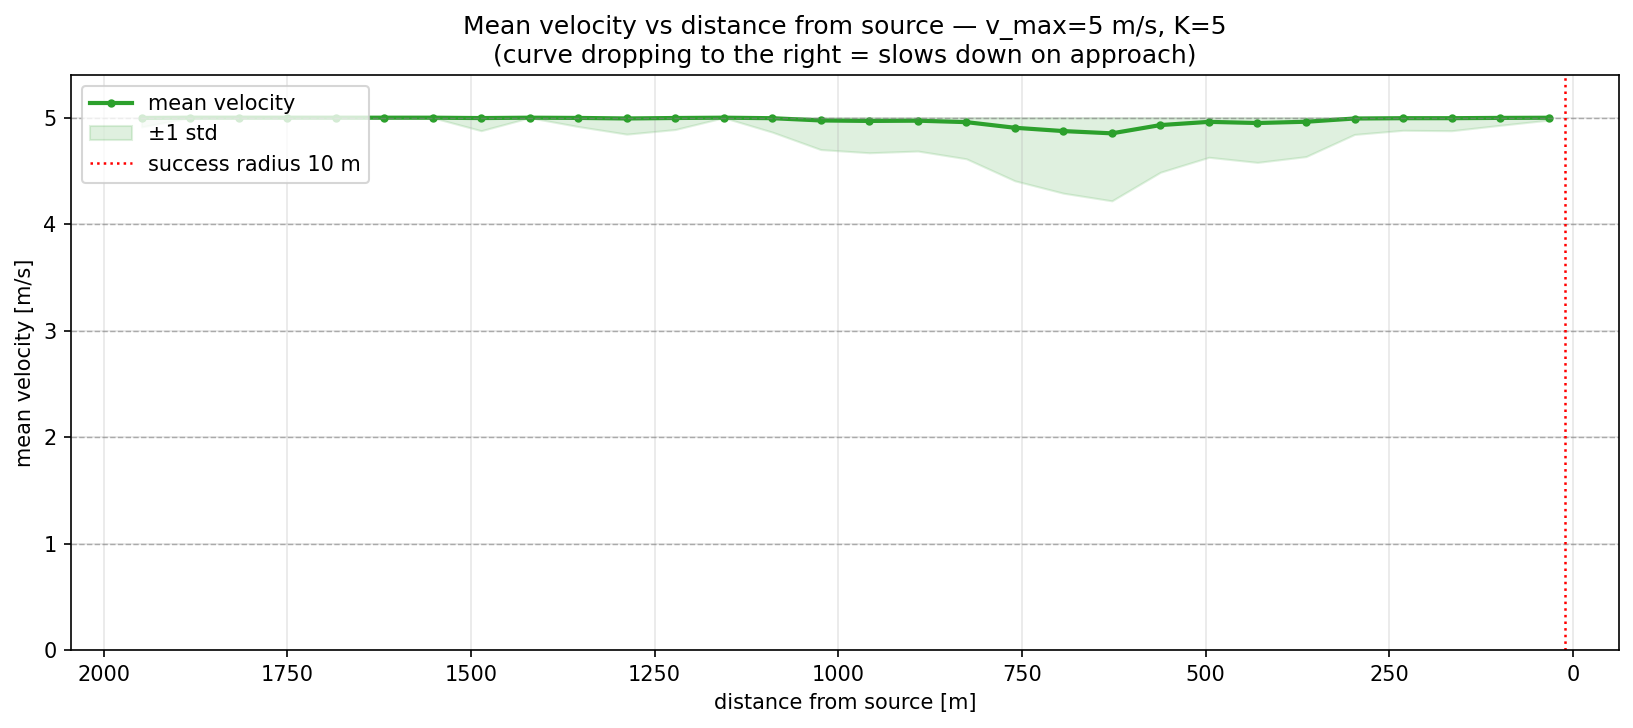
\includegraphics[width=\linewidth]{velocity_vs_distance.png}
    \caption{Velocit\`a media in funzione della distanza dalla sorgente (asse invertito:
             lontano a sinistra, vicino a destra; linea rossa = raggio di successo).}
  \end{subfigure}

  \vspace{6pt}
  \begin{subfigure}{0.78\linewidth}
    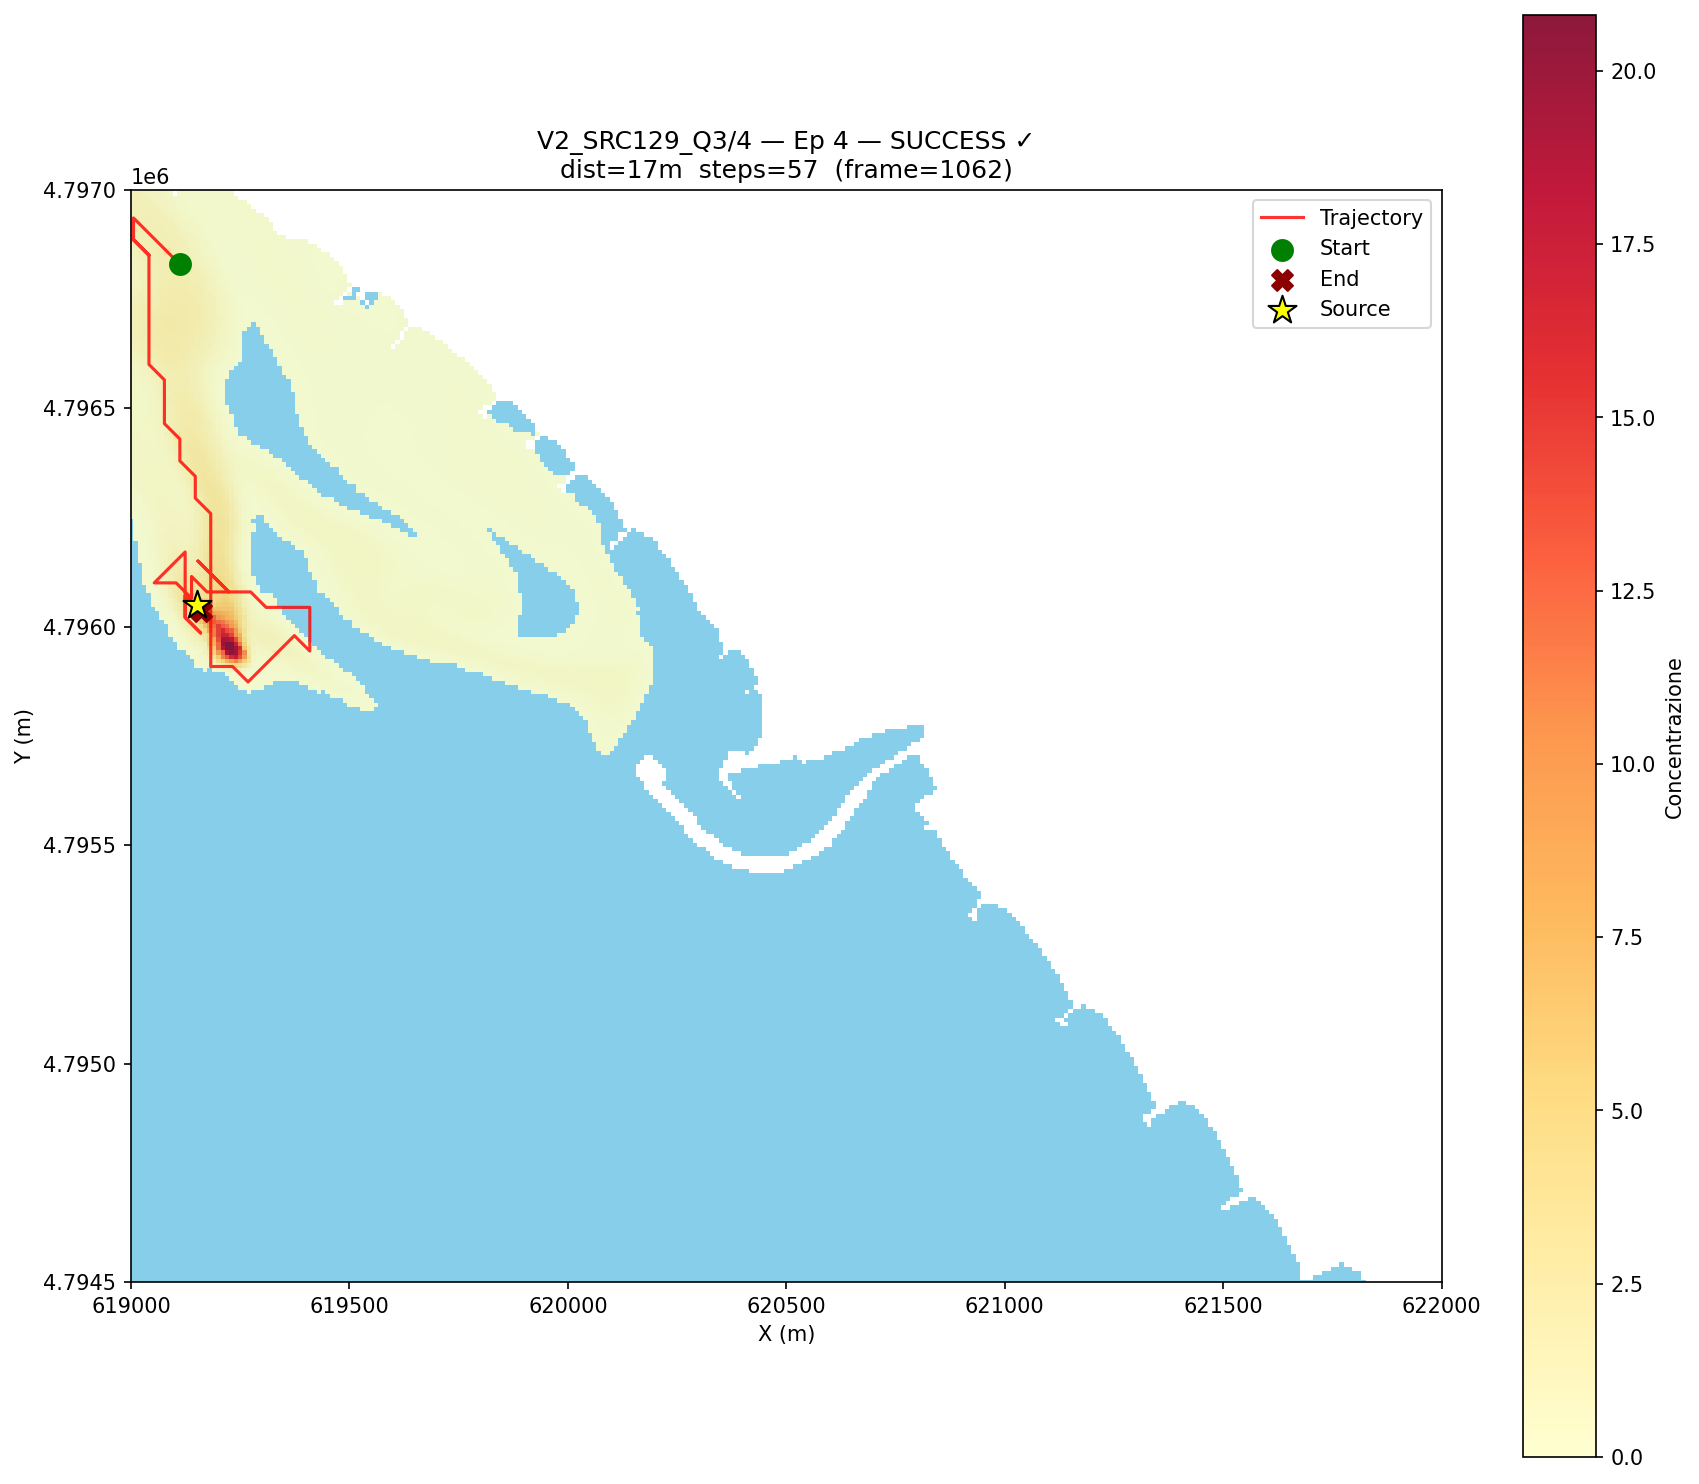
\includegraphics[width=\linewidth]{ep04_chunk2_trajectory.png}
    \caption{Traiettoria con manovra attorno alla sorgente: scavalcamenti e ri-approcci
             (57 step).}
  \end{subfigure}
  \caption{Esperimento a raggio $10\,\text{m}$. La velocit\`a media resta prossima al
           massimo a ogni distanza dalla sorgente (a): l'agente non frena. Scende invece
           lungo il plume a piena velocit\`a e \textbf{manovra ripetutamente} attorno alla
           sorgente (b) per far passare una falcata entro i $10\,\text{m}$.}
  \label{fig:r10traj}
\end{figure}

\subsection{Heatmap di occupazione dell'agente}
\label{sec:rl_heatmap}

Per un riscontro \emph{visivo} dei risultati numerici si riportano alcune \textbf{heatmap
di occupazione}: dato uno scenario (sorgente, vento, chunk) si eseguono 10 episodi e si
accumula la densit\`a di presenza dell'agente sul dominio, su sfondo geografico (mare,
costa, sorgente $\star$). Si confrontano tre agenti alla \textbf{stessa velocit\`a
massima}: FCM ($5\,\text{m/s}$), PPO a singola corona ($v_{\max}{=}5$) e PPO a doppia
corona ($v_{\max}{=}5$), su scenari \emph{difficili} (vento V1/V2, chunk Q1/2 o Q3/4). La
scala colori \`e \textbf{comune ai tre pannelli}, fissata sui due modelli PPO; l'FCM, che
oscilla a lungo negli stessi punti, ha densit\`a di picco molto pi\`u alte e quindi
\textbf{satura}.

\begin{figure}[H]
  \centering
  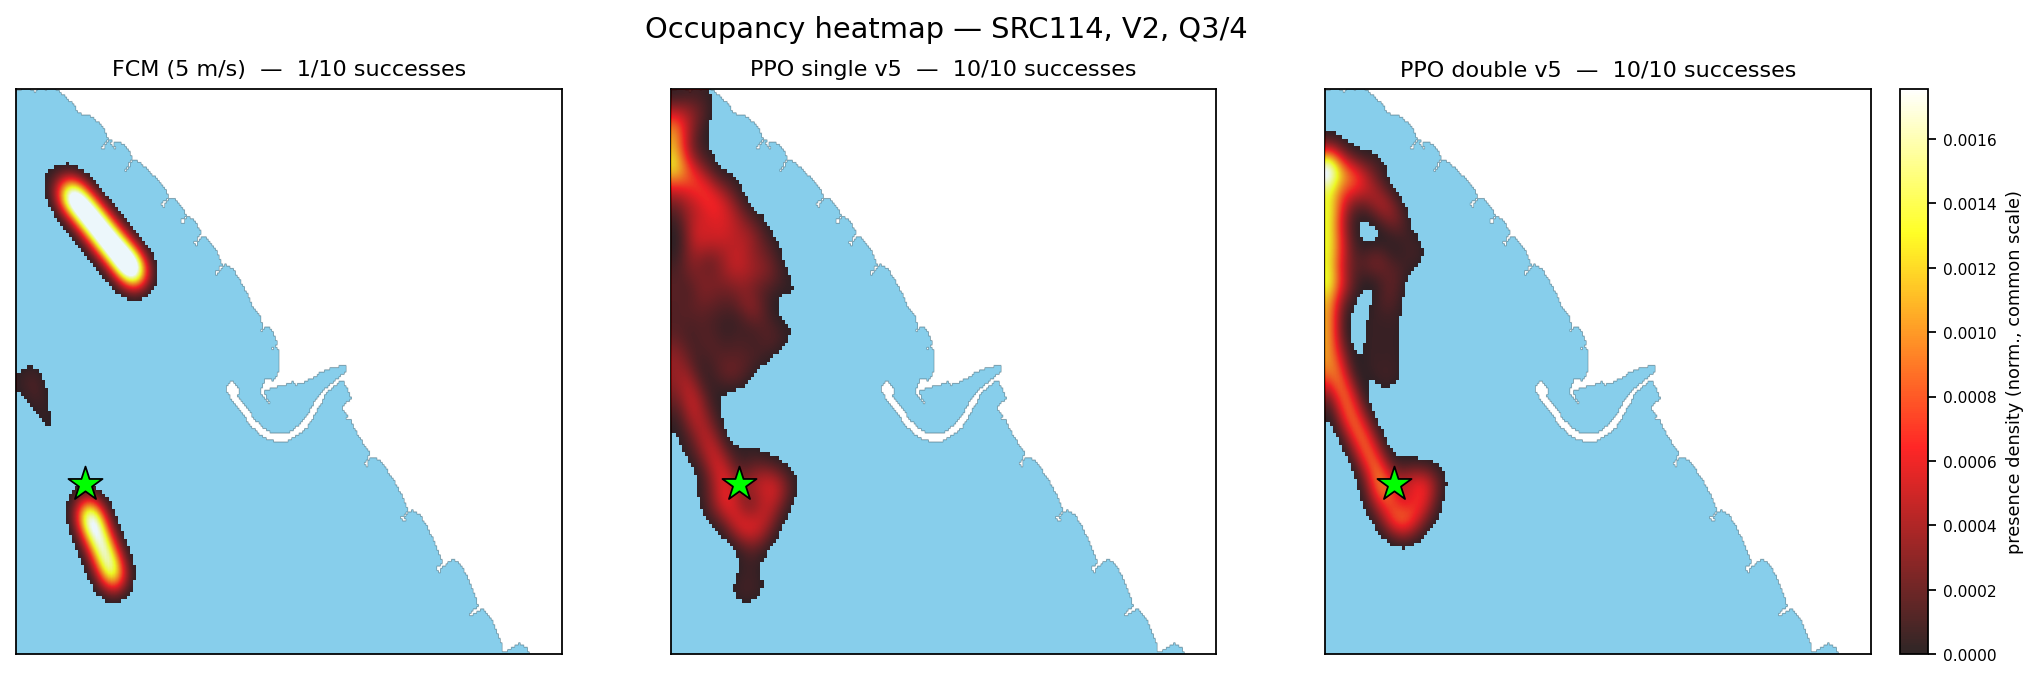
\includegraphics[width=\linewidth]{heatmap_1_SRC114_V2_Q2.png}
  \caption{Heatmap di occupazione --- SRC114, V2, Q3/4. FCM (sinistra) vs.\ PPO singola
           corona (centro) vs.\ PPO doppia corona (destra), $v_{\max}{=}5$, scala comune.}
  \label{fig:heatmap1}
\end{figure}

\begin{figure}[H]
  \centering
  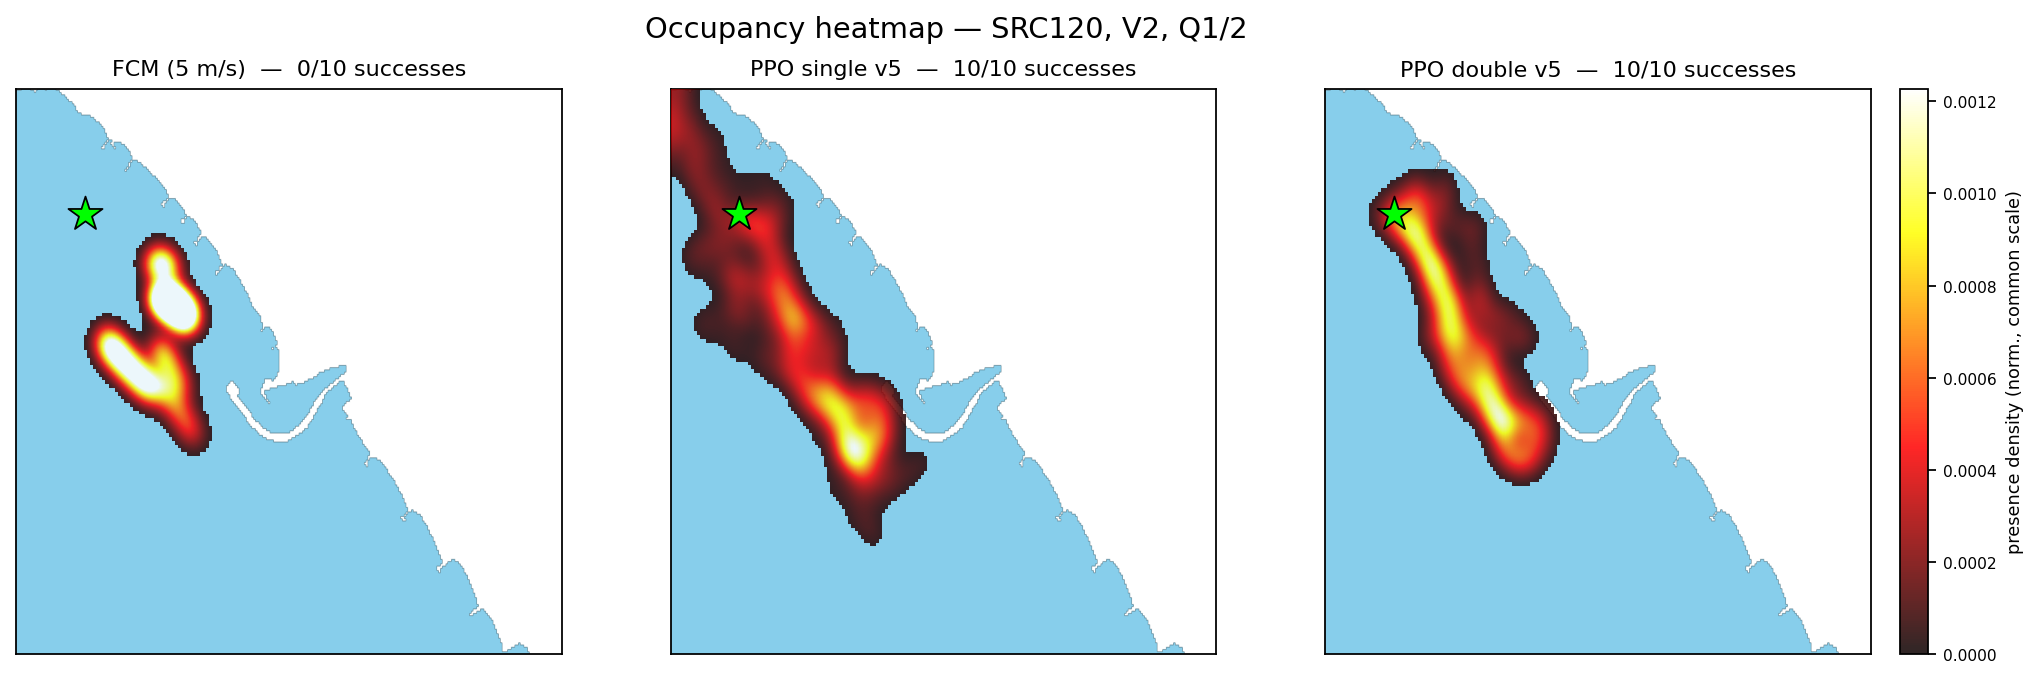
\includegraphics[width=\linewidth]{heatmap_2_SRC120_V2_Q1.png}
  \caption{Heatmap di occupazione --- SRC120, V2, Q1/2. Stessa disposizione e stessa scala
           della figura precedente.}
  \label{fig:heatmap2}
\end{figure}

Se ne leggono due fatti. Nel confronto \textbf{FCM vs.\ PPO}, l'FCM resta
\textbf{intrappolato} in macchie oscillanti lontane dalla sorgente e quasi sempre
fallisce, mentre il PPO forma una scia che \textbf{converge sulla sorgente}: \`e la
controparte visiva del divario di success rate (Sezione~\ref{sec:rl_confronto}) --- la
risalita di gradiente \emph{locale}, senza memoria n\'e contesto, si perde nel plume
avvettato. Nel confronto \textbf{singola vs.\ doppia corona}, entrambe raggiungono la
sorgente, ma la doppia concentra la presenza in un \textbf{corridoio pi\`u stretto e
definito} (pi\`u luminoso a parit\`a di scala) mentre la singola \`e pi\`u dispersa: \`e
la controparte visiva del $-34\%$ di step della Tabella~\ref{tab:dual_vmax}. Va letta con
un'avvertenza: la luminosit\`a indica la \emph{densit\`a di passaggio}, non la velocit\`a
--- un tratto pi\`u luminoso vicino alla sorgente riflette la convergenza di tutte le run
in un corridoio comune, non un rallentamento (la velocit\`a resta $\sim v_{\max}$).

\subsection{Analisi delle spawn map}
\label{sec:spawn_map}

Per indagare se l'esito di un episodio dipenda dalla posizione iniziale del master, sono
state generate le \textbf{spawn map} per le configurazioni vento--chunk con success rate
inferiore al 100\%. Per ciascuna si selezionano le 5 sorgenti con il maggior numero di
fallimenti; per ogni terna (sorgente, $v$, $q$) si eseguono 10 episodi e si registrano le
coordinate di spawn, contrassegnate con un \textcolor{green!60!black}{cerchio verde}
(successo) o una \textcolor{red!70!black}{croce rossa} (fallimento), sovrapposte al plume
di concentrazione della specifica sorgente all'istante $Q^*$.

\begin{figure}[H]
  \centering
  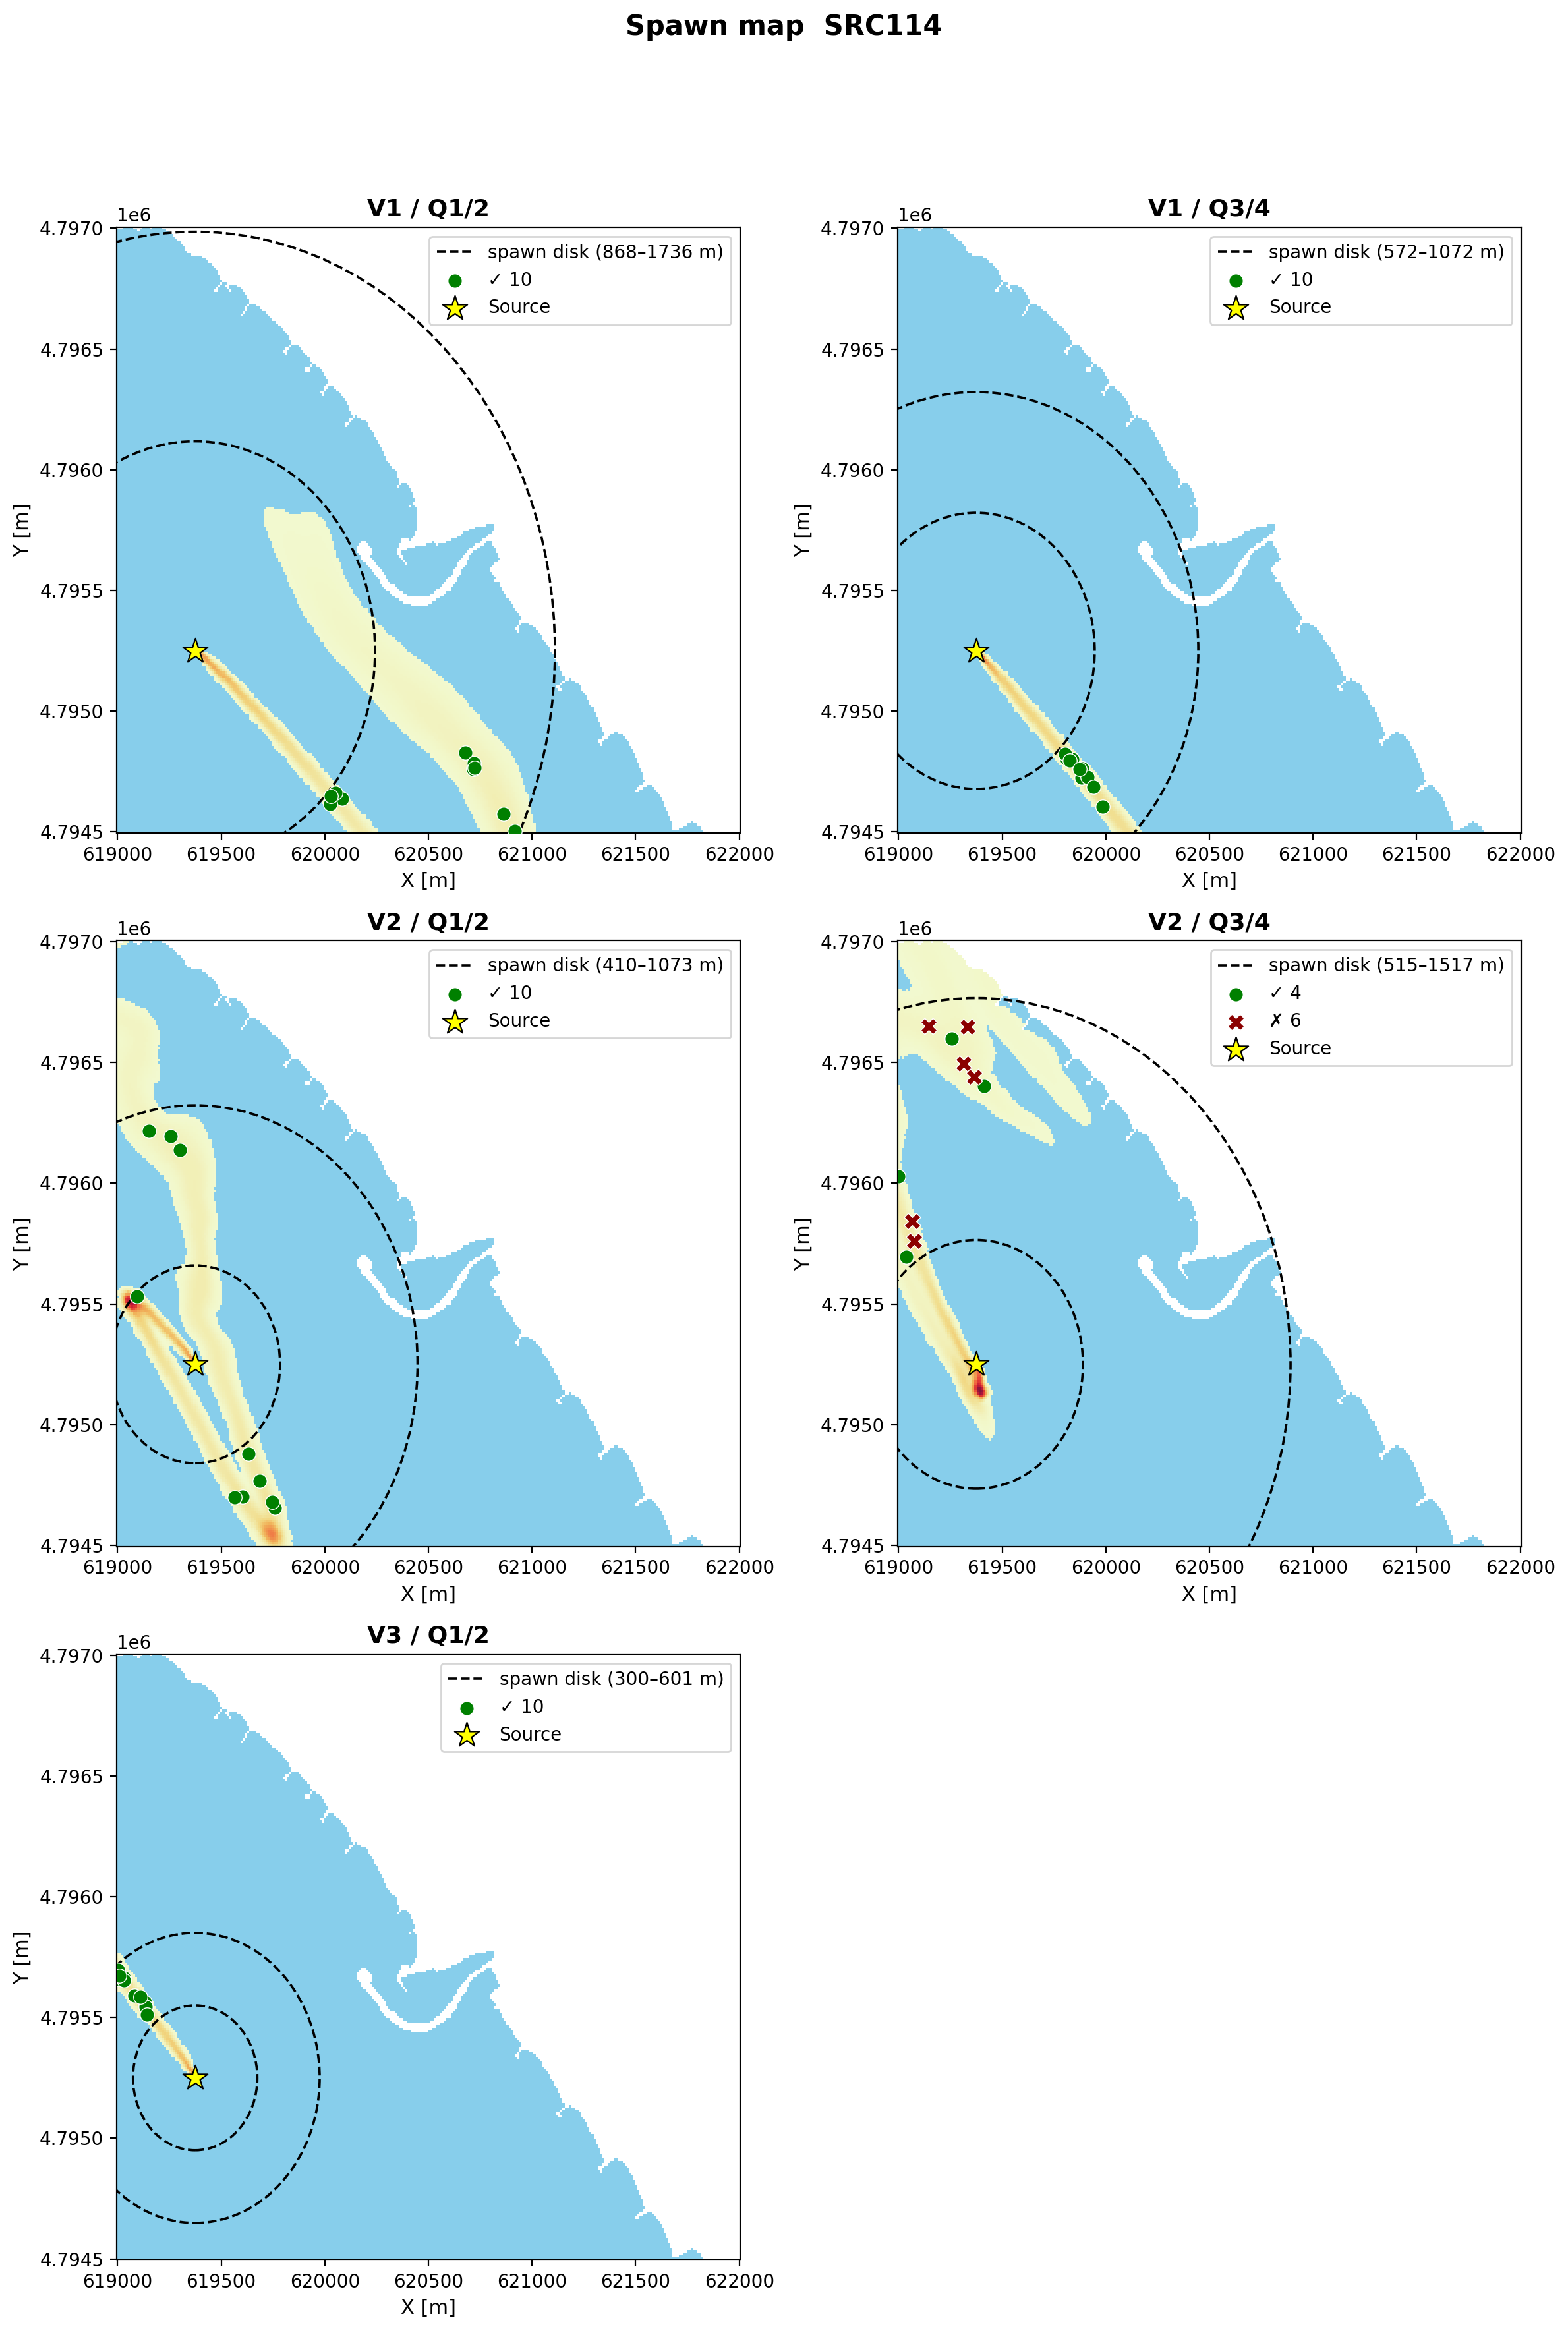
\includegraphics[width=\linewidth]{spawn_SRC114.png}
  \caption{Spawn map --- SRC114. Cerchi verdi (successo) e croci rosse (fallimento)
           risultano spazialmente intrecciati: non emerge alcuna regione di partenza
           sistematicamente sfavorevole.}
  \label{fig:spawn1}
\end{figure}

\begin{figure}[H]
  \centering
  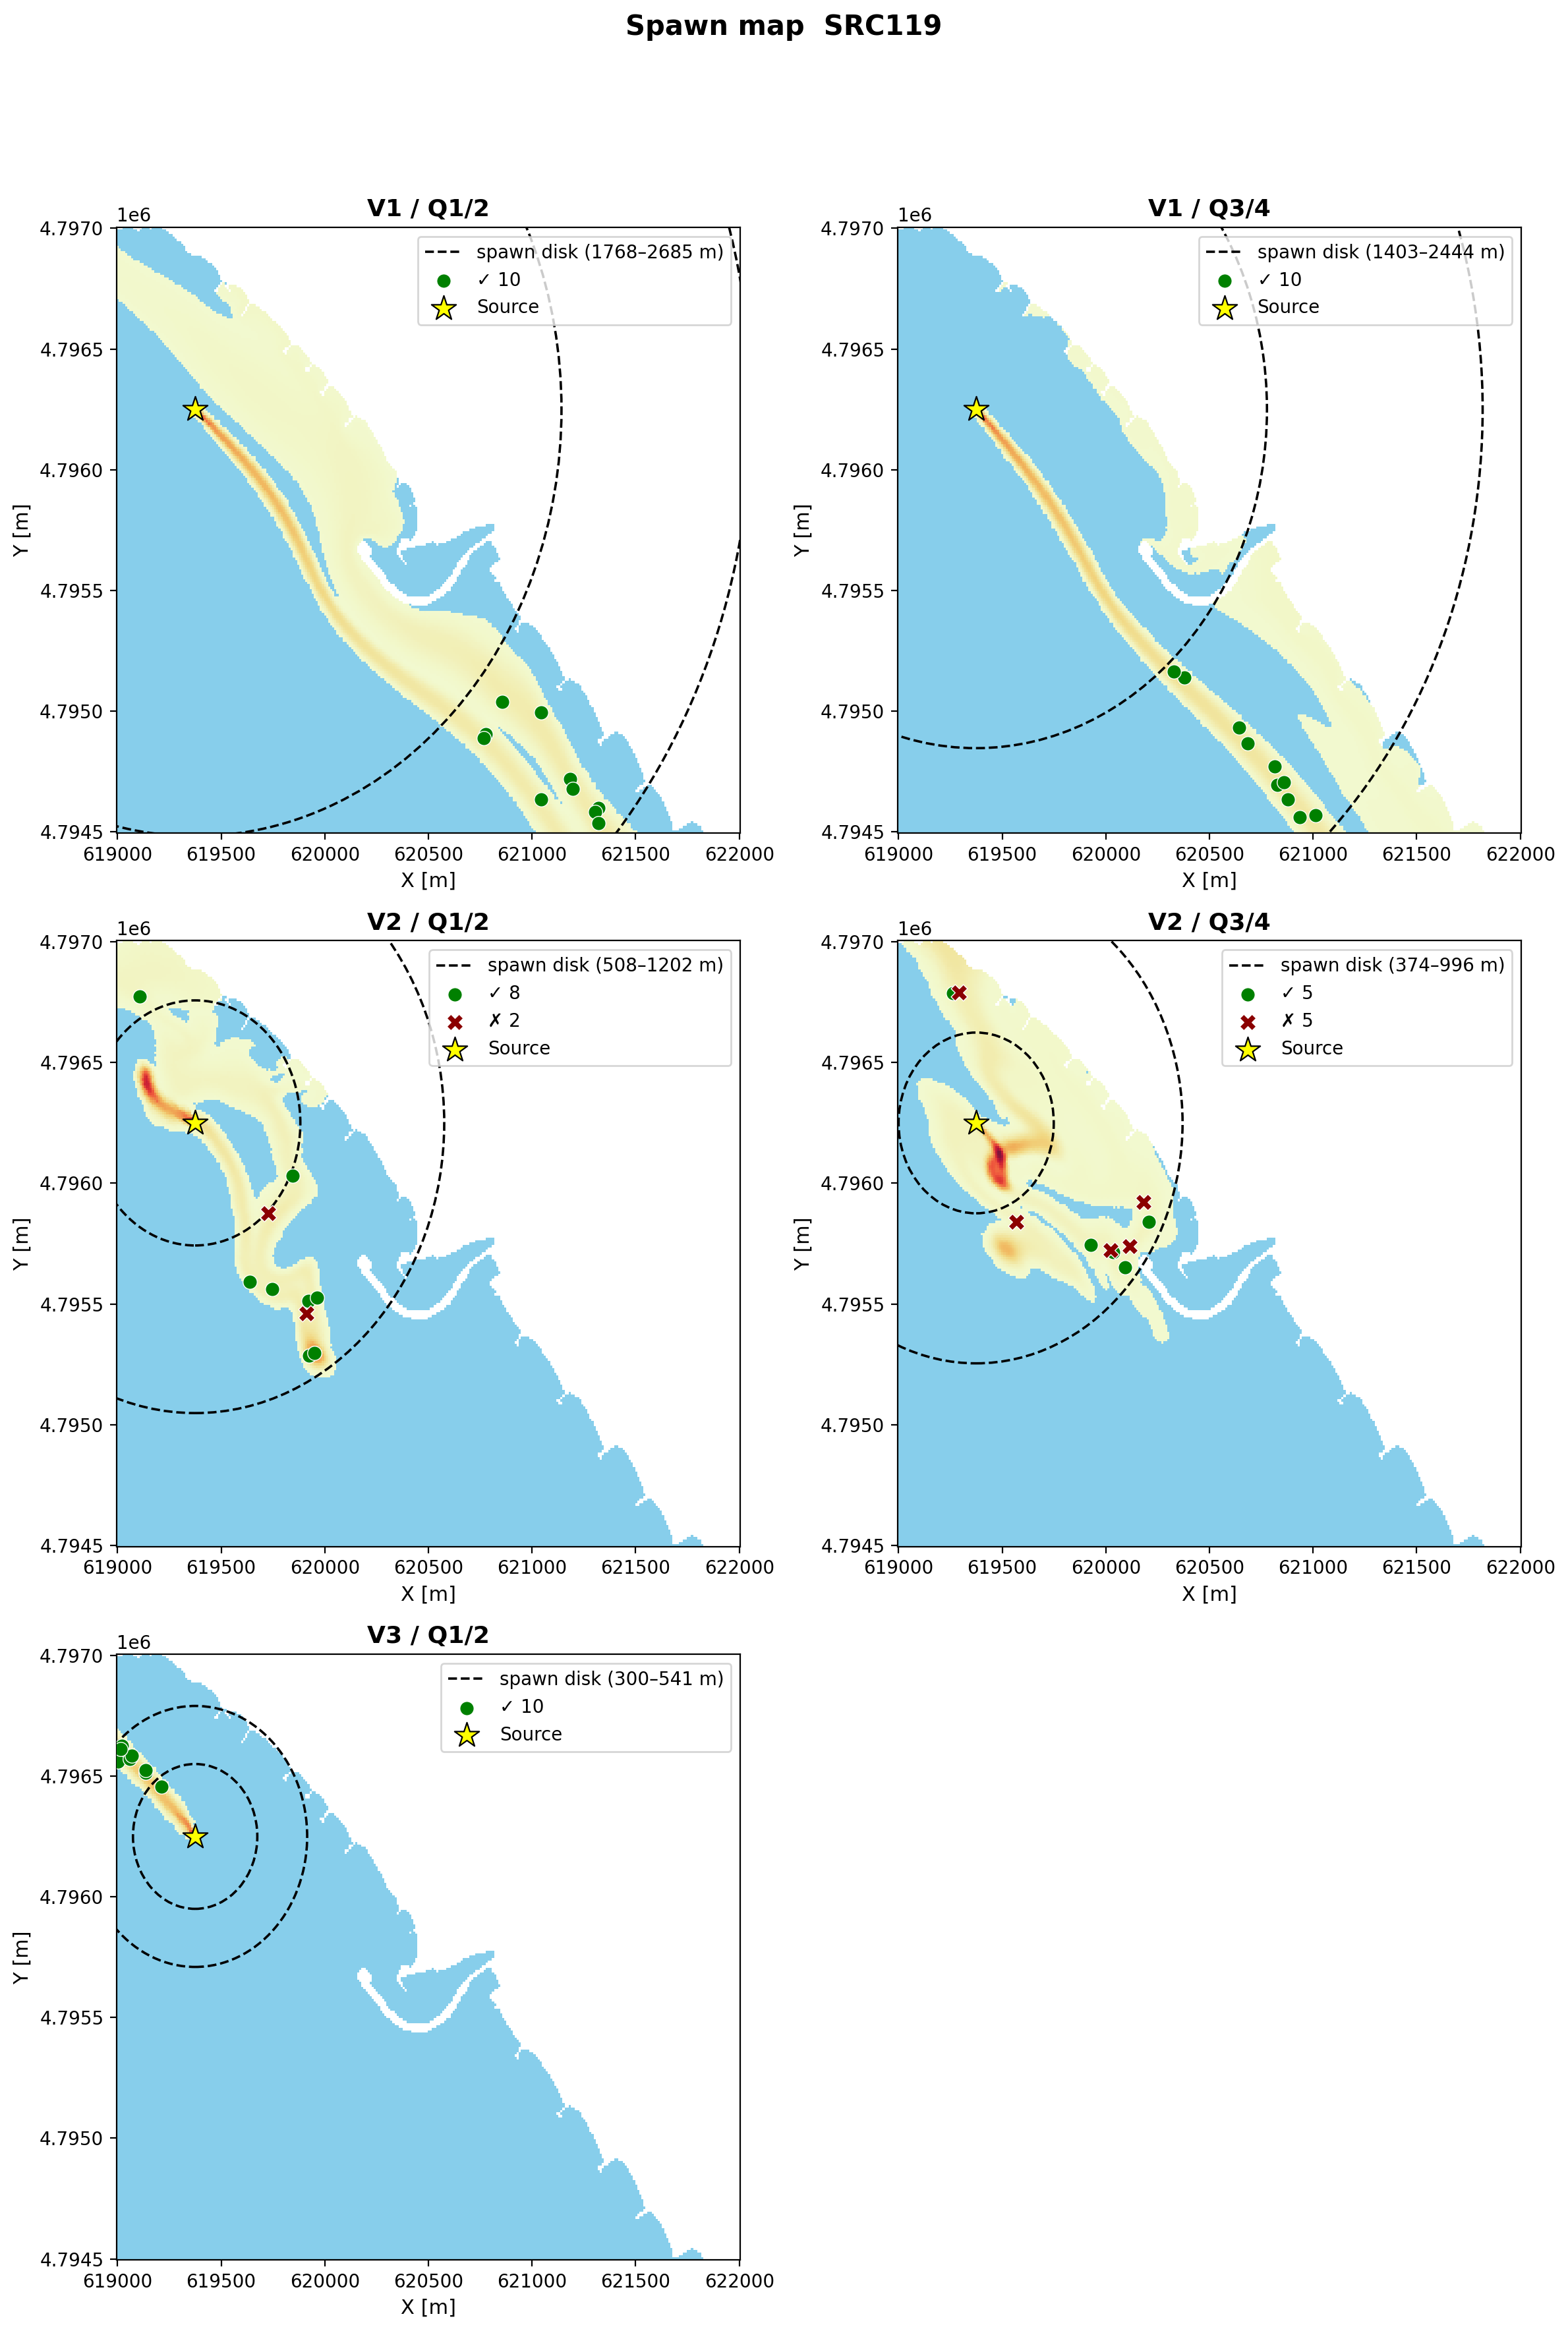
\includegraphics[width=\linewidth]{spawn_SRC119.png}
  \caption{Spawn map --- SRC119. Anche qui successi e fallimenti si alternano nelle stesse
           zone del plume: l'esito non \`e separabile in base alla posizione di spawn.}
  \label{fig:spawn2}
\end{figure}

\begin{figure}[H]
  \centering
  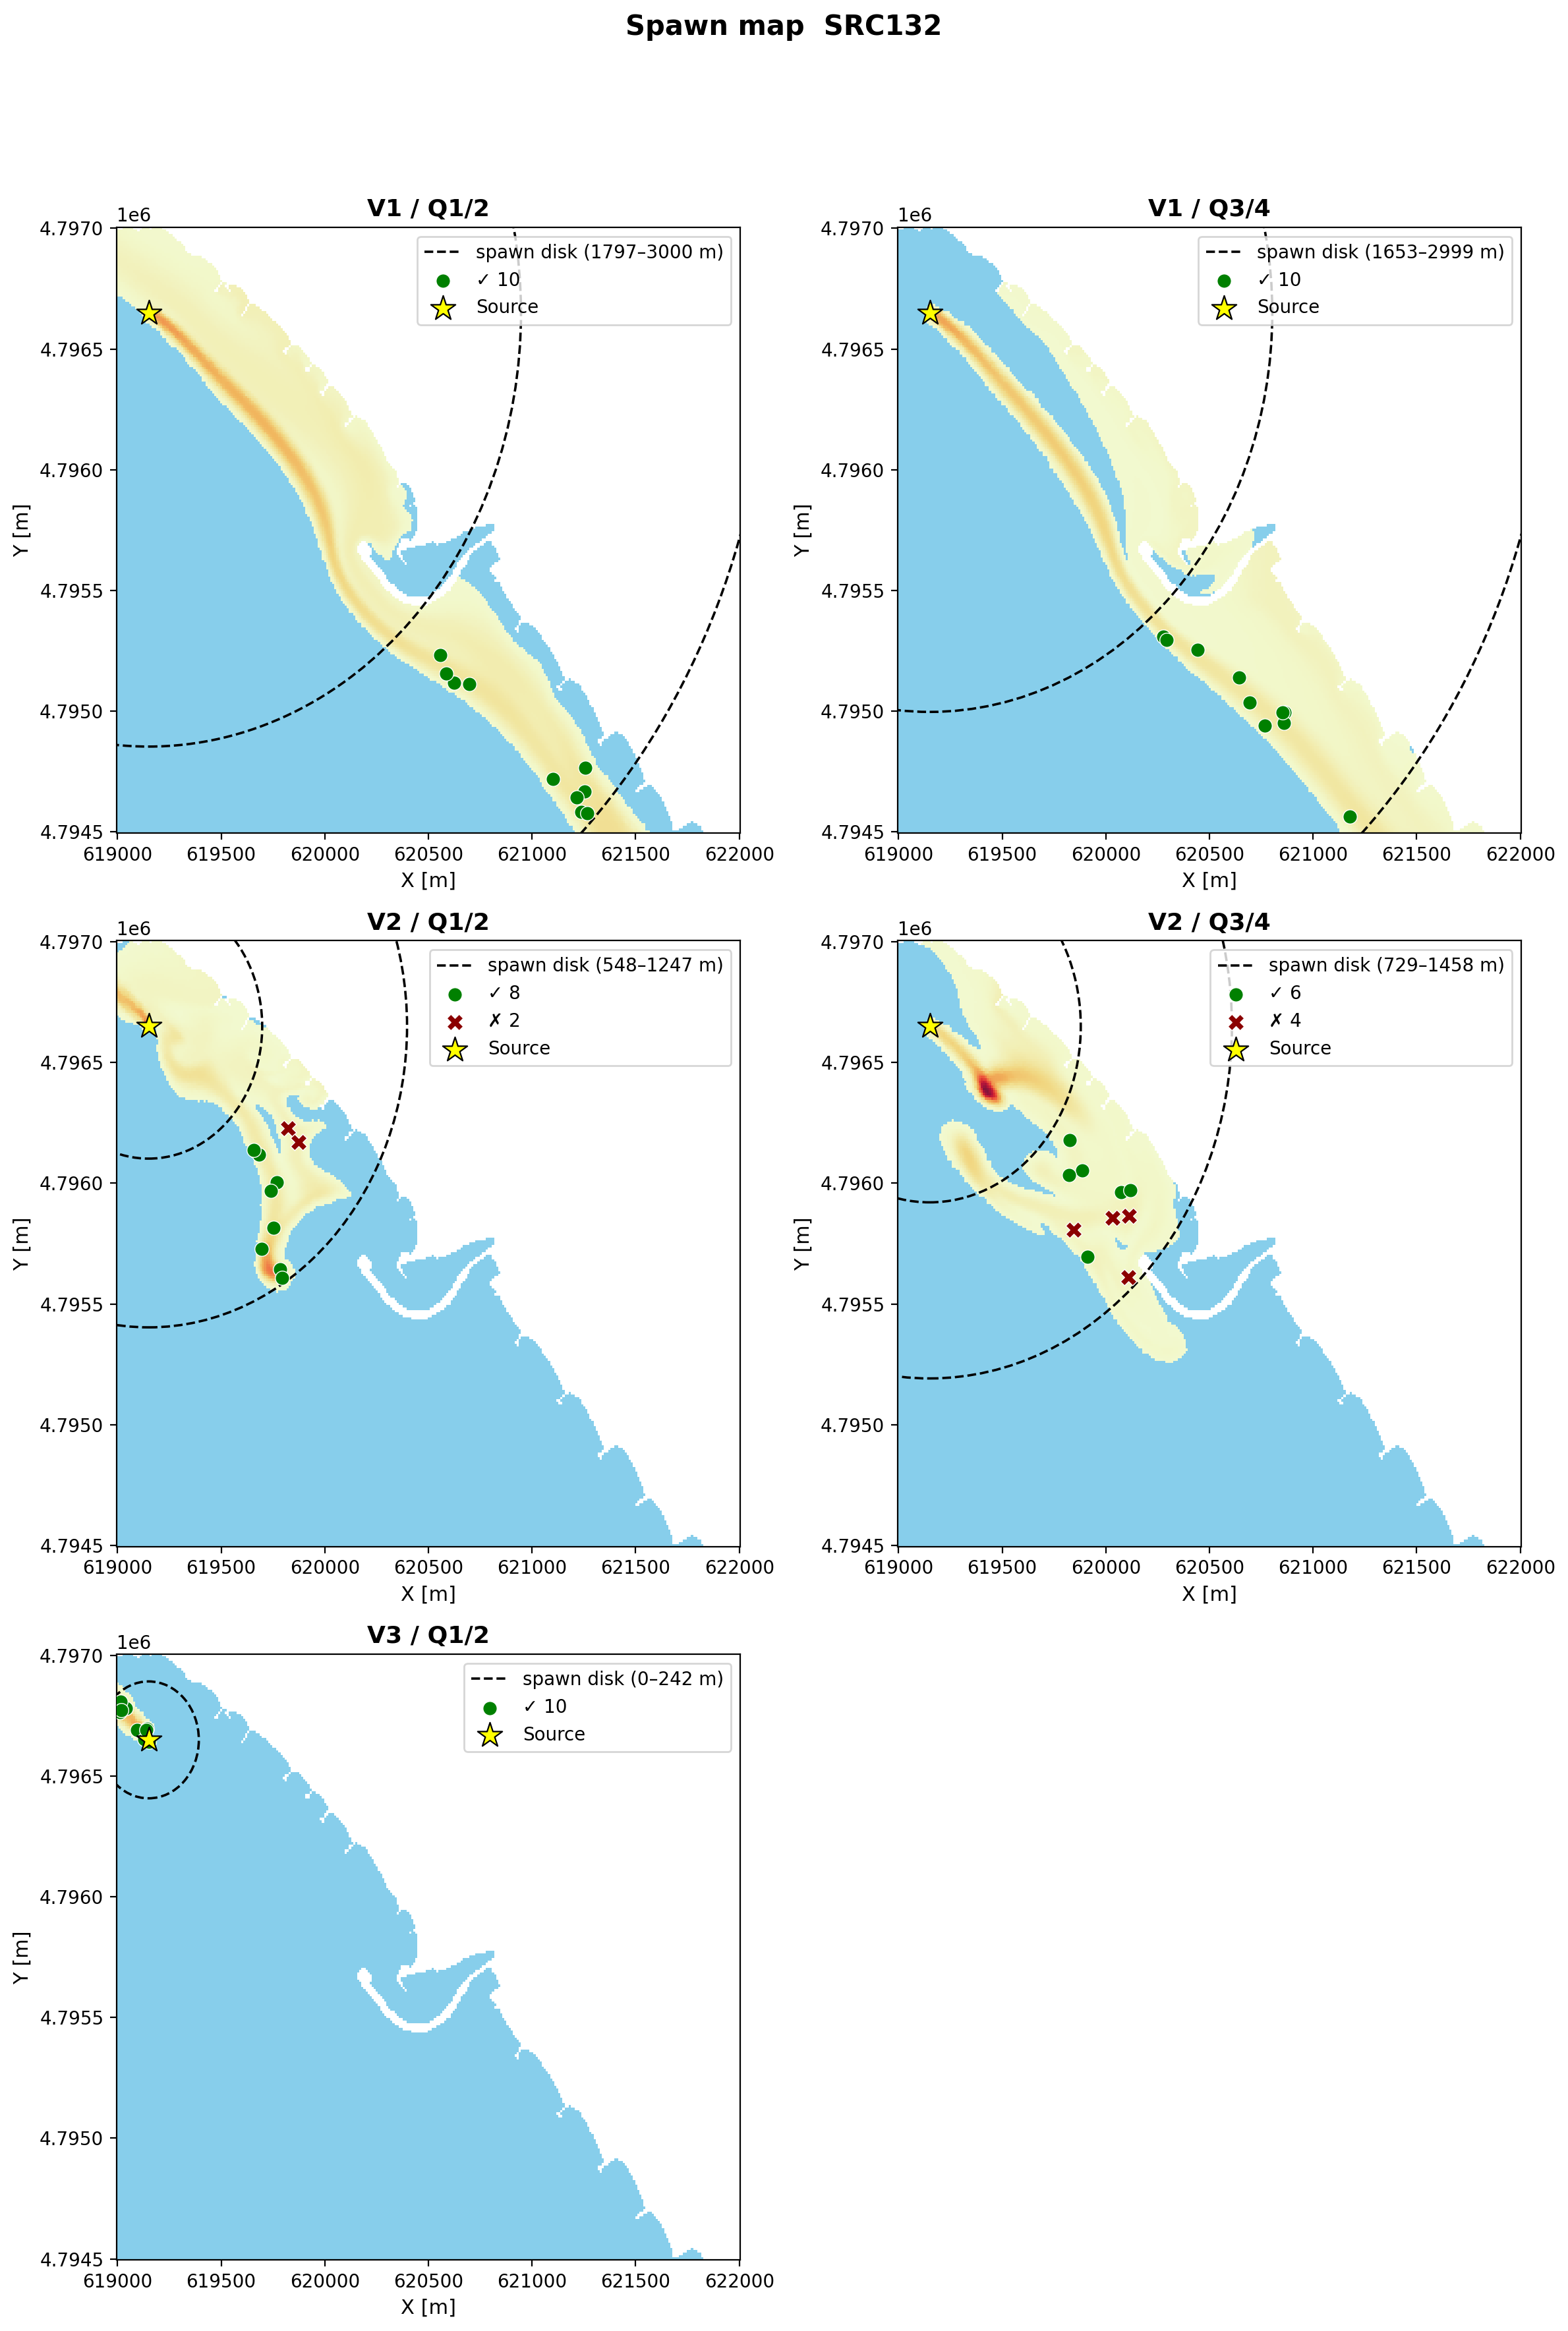
\includegraphics[width=\linewidth]{spawn_SRC132.png}
  \caption{Spawn map --- SRC132. La sovrapposizione di esiti opposti dagli stessi punti di
           partenza conferma che il fallimento dipende dalle condizioni idrodinamiche del
           chunk, non dalla geometria dello spawn.}
  \label{fig:spawn3}
\end{figure}

In tutte le sorgenti analizzate, i punti di partenza che portano al successo e quelli che
portano al fallimento \textbf{non mostrano alcuna separazione spaziale}: non emergono zone
di spawn sistematicamente ``difficili'' o ``facili''. L'esito di un episodio non dipende
dunque dalla posizione iniziale del master, bens\`i dalle condizioni idrodinamiche locali
(intensit\`a e direzione del plume, turbolenza) proprie di quel chunk temporale e di quello
scenario di vento. I fallimenti residui del modello sono da attribuire a caratteristiche
intrinseche degli scenari pi\`u difficili, non a limitazioni geometriche dello spazio di
spawn.

\subsection{Confronto con FCM puro e adattivo}
\label{sec:rl_confronto}

La Tabella~\ref{tab:confronto} riassume il confronto tra le due varianti del metodo del
gradiente (Capitolo~\ref{cap:fcm}) e il modello RL di riferimento (\texttt{minimal}),
valutati sulle stesse sorgenti di test.

\begin{table}[H]
\centering
\renewcommand{\arraystretch}{1.3}
\small
\begin{tabular}{L{3.2cm} C{2.8cm} C{2.8cm} C{2.8cm}}
\toprule
\rowcolor{headerbg}
\textcolor{white}{\textbf{Metrica}} &
\textcolor{white}{\textbf{FCM puro}} &
\textcolor{white}{\textbf{FCM adattivo}} &
\textcolor{white}{\textbf{RL (minimal)}} \\
\midrule
\rowcolor{rowalt}
SR globale & 32{,}9\% & 63{,}5\% & \textbf{96{,}9\%} \\
V0 & 39{,}7\% & 84{,}6\% & \textbf{100{,}0\%} \\
\rowcolor{rowalt}
V1 & 16{,}0\% & 35{,}3\% & \textbf{99{,}0\%} \\
V2 & 23{,}7\% & 41{,}7\% & \textbf{88{,}7\%} \\
\rowcolor{rowalt}
V3 & 51{,}9\% & 92{,}3\% & \textbf{99{,}7\%} \\
Q1/4 & 50{,}5\% & 90{,}9\% & \textbf{100{,}0\%} \\
\rowcolor{rowalt}
Q1/2 & 11{,}5\% & 44{,}2\% & \textbf{93{,}5\%} \\
Q3/4 & 36{,}5\% & 55{,}3\% & \textbf{97{,}1\%} \\
\bottomrule
\end{tabular}
\caption{Confronto diretto tra FCM puro ($r_s{=}50\,\text{m}$), FCM con passo adattivo
         nella configurazione migliore ($lr{=}40\,\text{m}$,
         Tabella~\ref{tab:fcm_sweep}) e modello RL di riferimento \texttt{minimal}. Il FCM
         adattivo adotta il disco adattivo di spawn, mentre il FCM puro e l'RL
         \texttt{minimal} usano la cascata (Sezione~\ref{sec:spawn}); il confronto RL vs.\ FCM
         a parit\`a di spawn e velocit\`a \`e nella Sezione~\ref{sec:rl_fullrange}.}
\label{tab:confronto}
\end{table}

Il modello RL supera nettamente entrambe le varianti del metodo del gradiente su ogni
scenario: $+64$ punti percentuali sul success rate globale rispetto al FCM puro e $+33$
rispetto al FCM adattivo. Il divario \`e massimo proprio negli scenari a plume diffuso
(V1, V2, Q1/2), dove il gradiente locale degenera e i metodi reattivi perdono la
direzione.

Il confronto della Tabella~\ref{tab:confronto} \`e per giunta \emph{sfavorevole} all'RL
sul piano cinematico: il modello \texttt{minimal} si muove a passo fisso di
$10\,\text{m}$ per timestep ($1\,\text{m/s}$), mentre l'FCM adattivo a $lr = 40\,\text{m}$
compie passi fino a quattro volte pi\`u lunghi ($4\,\text{m/s}$). L'RL vince dunque pur
essendo quattro volte pi\`u lento. Poich\'e entrambi i metodi dispongono ora di una
versione a velocit\`a variabile --- la catena della Sezione~\ref{sec:rl_velocity} per il
PPO, lo sweep su $lr$ per l'FCM --- \`e possibile un confronto \textbf{a parit\`a di
velocit\`a massima}, che neutralizza questo fattore: un passo FCM di $lr$ metri per
timestep corrisponde a $lr/10$ m/s, e si accoppia quindi con lo stadio PPO di pari
$v_{\max}$ (Tabella~\ref{tab:fcm_ppo_vel}).

\begin{table}[H]
\centering
\renewcommand{\arraystretch}{1.35}
\setlength{\tabcolsep}{4pt}
\small
\begin{tabular}{l c c c c c c c c}
\toprule
\rowcolor{headerbg}
\textcolor{white}{\textbf{Vel.\ / metodo}} &
\textcolor{white}{\textbf{SR\%}} &
\textcolor{white}{\textbf{V0}} &
\textcolor{white}{\textbf{V1}} &
\textcolor{white}{\textbf{V2}} &
\textcolor{white}{\textbf{V3}} &
\textcolor{white}{\textbf{Q1/4}} &
\textcolor{white}{\textbf{Q1/2}} &
\textcolor{white}{\textbf{Q3/4}} \\
\midrule
FCM ($lr{=}10$) & 54{,}6 & 73{,}7 & 29{,}5 & 35{,}9 & 79{,}5 & 77{,}9 & 30{,}3 & 55{,}8 \\
\rowcolor{rowalt}
PPO ($v_{\max}{=}1$) & \shortstack{97{,}1\\[-1pt]{\scriptsize\textcolor{green!50!black}{+42{,}5}}} & \shortstack{99{,}5\\[-1pt]{\scriptsize\textcolor{green!50!black}{+25{,}8}}} & \shortstack{100{,}0\\[-1pt]{\scriptsize\textcolor{green!50!black}{+70{,}5}}} & \shortstack{89{,}7\\[-1pt]{\scriptsize\textcolor{green!50!black}{+53{,}8}}} & \shortstack{99{,}2\\[-1pt]{\scriptsize\textcolor{green!50!black}{+19{,}7}}} & \shortstack{100{,}0\\[-1pt]{\scriptsize\textcolor{green!50!black}{+22{,}1}}} & \shortstack{95{,}0\\[-1pt]{\scriptsize\textcolor{green!50!black}{+64{,}7}}} & \shortstack{96{,}3\\[-1pt]{\scriptsize\textcolor{green!50!black}{+40{,}6}}} \\
\midrule
FCM ($lr{=}20$) & 58{,}2 & 80{,}1 & 32{,}1 & 34{,}6 & 85{,}9 & 81{,}7 & 38{,}0 & 54{,}8 \\
\rowcolor{rowalt}
PPO ($v_{\max}{=}2$) & \shortstack{99{,}7\\[-1pt]{\scriptsize\textcolor{green!50!black}{+41{,}5}}} & \shortstack{100{,}0\\[-1pt]{\scriptsize\textcolor{green!50!black}{+19{,}9}}} & \shortstack{99{,}5\\[-1pt]{\scriptsize\textcolor{green!50!black}{+67{,}4}}} & \shortstack{99{,}2\\[-1pt]{\scriptsize\textcolor{green!50!black}{+64{,}6}}} & \shortstack{100{,}0\\[-1pt]{\scriptsize\textcolor{green!50!black}{+14{,}1}}} & \shortstack{100{,}0\\[-1pt]{\scriptsize\textcolor{green!50!black}{+18{,}3}}} & \shortstack{99{,}0\\[-1pt]{\scriptsize\textcolor{green!50!black}{+61{,}1}}} & \shortstack{100{,}0\\[-1pt]{\scriptsize\textcolor{green!50!black}{+45{,}2}}} \\
\midrule
FCM ($lr{=}30$) & 60{,}7 & 84{,}6 & 30{,}8 & 37{,}2 & 90{,}4 & 86{,}1 & 39{,}4 & 56{,}7 \\
\rowcolor{rowalt}
PPO ($v_{\max}{=}3$) & \shortstack{99{,}9\\[-1pt]{\scriptsize\textcolor{green!50!black}{+39{,}2}}} & \shortstack{100{,}0\\[-1pt]{\scriptsize\textcolor{green!50!black}{+15{,}4}}} & \shortstack{100{,}0\\[-1pt]{\scriptsize\textcolor{green!50!black}{+69{,}2}}} & \shortstack{99{,}7\\[-1pt]{\scriptsize\textcolor{green!50!black}{+62{,}6}}} & \shortstack{100{,}0\\[-1pt]{\scriptsize\textcolor{green!50!black}{+9{,}6}}} & \shortstack{100{,}0\\[-1pt]{\scriptsize\textcolor{green!50!black}{+13{,}9}}} & \shortstack{99{,}8\\[-1pt]{\scriptsize\textcolor{green!50!black}{+60{,}4}}} & \shortstack{100{,}0\\[-1pt]{\scriptsize\textcolor{green!50!black}{+43{,}3}}} \\
\midrule
FCM ($lr{=}40$) & 63{,}5 & 84{,}6 & 35{,}3 & 41{,}7 & 92{,}3 & 90{,}9 & 44{,}2 & 55{,}3 \\
\rowcolor{rowalt}
PPO ($v_{\max}{=}4$) & \shortstack{99{,}9\\[-1pt]{\scriptsize\textcolor{green!50!black}{+36{,}4}}} & \shortstack{100{,}0\\[-1pt]{\scriptsize\textcolor{green!50!black}{+15{,}4}}} & \shortstack{100{,}0\\[-1pt]{\scriptsize\textcolor{green!50!black}{+64{,}7}}} & \shortstack{99{,}5\\[-1pt]{\scriptsize\textcolor{green!50!black}{+57{,}8}}} & \shortstack{100{,}0\\[-1pt]{\scriptsize\textcolor{green!50!black}{+7{,}7}}} & \shortstack{100{,}0\\[-1pt]{\scriptsize\textcolor{green!50!black}{+9{,}1}}} & \shortstack{100{,}0\\[-1pt]{\scriptsize\textcolor{green!50!black}{+55{,}8}}} & \shortstack{99{,}6\\[-1pt]{\scriptsize\textcolor{green!50!black}{+44{,}3}}} \\
\midrule
FCM ($lr{=}50$) & 62{,}2 & 84{,}6 & 34{,}6 & 37{,}2 & 92{,}3 & 89{,}4 & 41{,}8 & 55{,}3 \\
\rowcolor{rowalt}
PPO ($v_{\max}{=}5$) & \shortstack{99{,}9\\[-1pt]{\scriptsize\textcolor{green!50!black}{+37{,}8}}} & \shortstack{100{,}0\\[-1pt]{\scriptsize\textcolor{green!50!black}{+15{,}4}}} & \shortstack{100{,}0\\[-1pt]{\scriptsize\textcolor{green!50!black}{+65{,}4}}} & \shortstack{99{,}7\\[-1pt]{\scriptsize\textcolor{green!50!black}{+62{,}6}}} & \shortstack{100{,}0\\[-1pt]{\scriptsize\textcolor{green!50!black}{+7{,}7}}} & \shortstack{100{,}0\\[-1pt]{\scriptsize\textcolor{green!50!black}{+10{,}6}}} & \shortstack{100{,}0\\[-1pt]{\scriptsize\textcolor{green!50!black}{+58{,}2}}} & \shortstack{99{,}8\\[-1pt]{\scriptsize\textcolor{green!50!black}{+44{,}5}}} \\
\bottomrule
\end{tabular}
\caption{FCM adattivo vs.\ PPO adattivo \textbf{a parit\`a di velocit\`a massima} (FCM:
         $lr/\Delta t$; PPO: $v_{\max}$), per scenario di vento (V) e chunk temporale (Q).
         Sotto ogni valore PPO, in verde, il surplus sul FCM in punti percentuali.}
\label{tab:fcm_ppo_vel}
\end{table}

Neutralizzato il fattore cinematico, il quadro non cambia: a \textbf{ogni} livello di
velocit\`a il PPO supera l'FCM di $36$--$42$ punti di success rate globale, e il divario
resta massimo negli scenari avversi (V1, V2, Q1/2), dove tocca i $55$--$70$ punti. Il
vantaggio dell'RL non \`e dunque un artefatto della velocit\`a: \`e strutturale. L'RL ha
appreso strategie non riducibili al gradiente locale --- sfruttamento della memoria
storica, navigazione in zone a bassa concentrazione, recupero da situazioni di stallo ---
che emergono dall'ottimizzazione su milioni di episodi e non sono accessibili a un metodo
che decide passo-passo senza contesto.

\subsection{Estensione all'intero range di velocit\`a}
\label{sec:rl_fullrange}

Le analisi precedenti coprono i valori interi $v_{\max} \in \{1,\ldots,5\}\,\text{m/s}$.
Per completare il quadro sull'\emph{intero} intervallo operativo del veicolo, la catena
\`e stata estesa sia verso il basso, con le \textbf{velocit\`a ridotte}
$v_{\max} \in \{0{,}1,\,0{,}4,\,0{,}7\}$, sia negli \textbf{stadi intermedi}
$v_{\max} \in \{1{,}2,\,1{,}5,\,1{,}7,\,1{,}9\}$, per entrambe le formazioni (singola e
doppia corona). Ogni stadio \`e ottenuto per fine-tuning a catena dal modello adiacente
gi\`a addestrato --- ascendente per gli intermedi, discendente per i valori bassi --- e
valutato sui consueti 1560 episodi held-out. In parallelo, il metodo del gradiente
adattivo \`e stato valutato al learning rate corrispondente ($lr = 10\,v_{\max}$, cfr.\
Sezione~\ref{sec:fcm_adam}) su tutte le stesse velocit\`a, cos\`i da estendere il confronto
\emph{a parit\`a di velocit\`a massima} lungo l'intero range. Le
Figure~\ref{fig:fullrange_sr}--\ref{fig:fullrange_steps} riportano l'andamento di success
rate e step medi al successo; la Tabella~\ref{tab:fullrange} ne raccoglie i valori.

\begin{figure}[H]
  \centering
  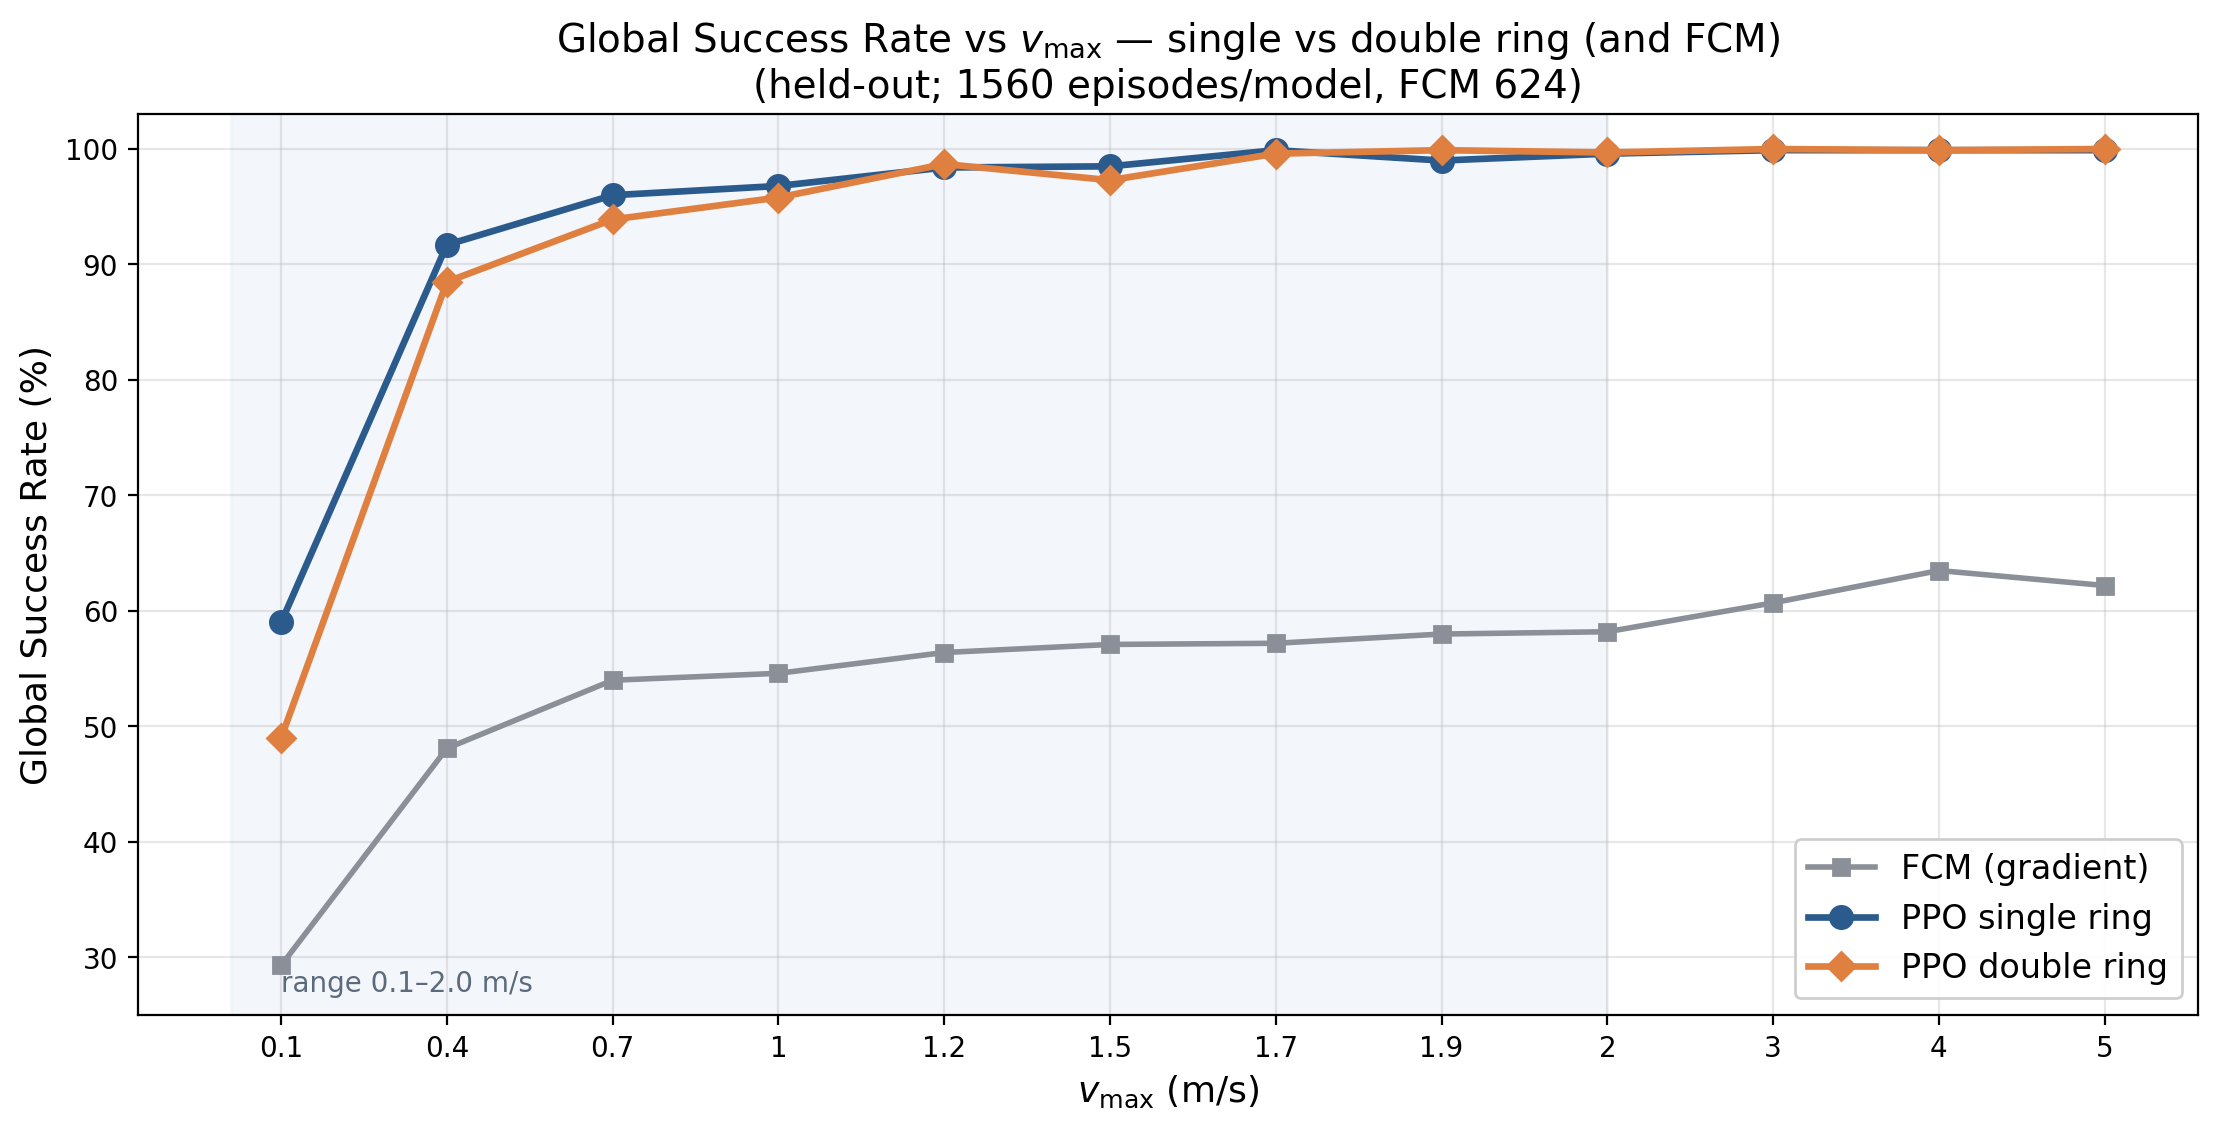
\includegraphics[width=0.95\linewidth]{sr_vs_vmax_single_double.png}
  \caption{Success rate globale in funzione di $v_{\max}$ sull'intero range
           ($0{,}1$--$5\,\text{m/s}$): PPO singola corona, PPO doppia corona e FCM adattivo
           (held-out; 1560 episodi per modello, 624 per l'FCM). Le due curve PPO saturano
           gi\`a a $v_{\max} \gtrsim 1{,}2$, mentre l'FCM resta confinato attorno al
           $55$--$63\%$ alle velocit\`a operative, con un ulteriore calo (fino al
           $\sim$$29\%$) a quelle pi\`u basse.}
  \label{fig:fullrange_sr}
\end{figure}

\begin{figure}[H]
  \centering
  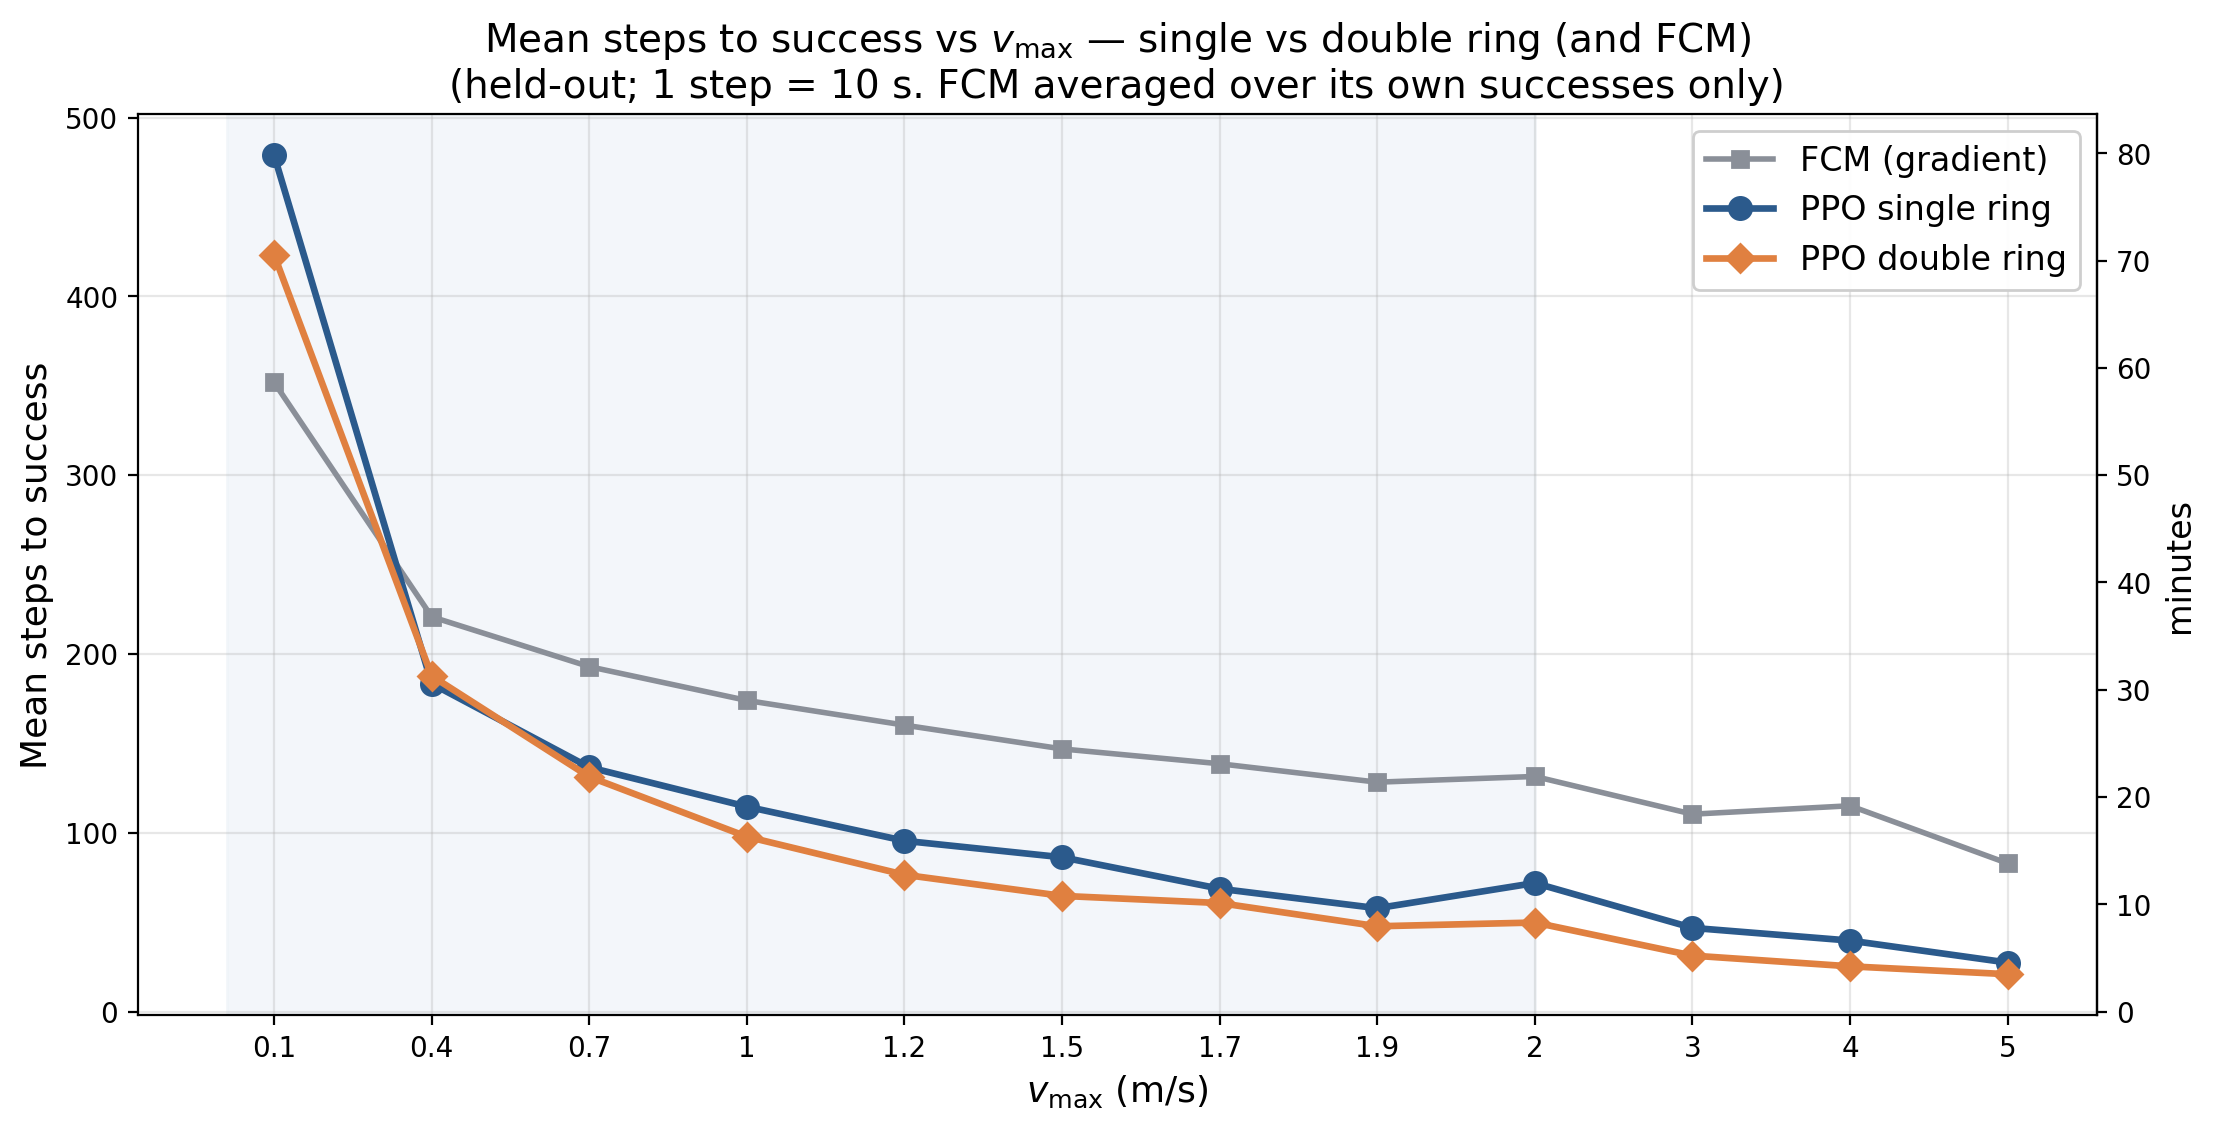
\includegraphics[width=0.95\linewidth]{steps_vs_vmax_single_double.png}
  \caption{Step medi al successo in funzione di $v_{\max}$ (asse secondario in minuti,
           $1\,\text{step}=10\,\text{s}$). Dalla velocit\`a nominale ($1\,\text{m/s}$) in su
           la doppia corona raggiunge la sorgente in meno passi della singola; alle
           velocit\`a pi\`u basse i due profili sono sostanzialmente sovrapposti. Il tempo al
           successo cala in modo netto all'aumentare di $v_{\max}$.}
  \label{fig:fullrange_steps}
\end{figure}

La Tabella~\ref{tab:fullrange_singledouble} dettaglia il confronto \emph{singola vs.\ doppia
corona} a ciascuna velocit\`a, riportando per entrambe success rate e passi al successo con
le rispettive differenze.

\begin{table}[H]
\centering
\renewcommand{\arraystretch}{0.95}
\setlength{\tabcolsep}{4pt}
\footnotesize
\begin{tabular}{c c c c c c c}
\toprule
\rowcolor{headerbg}
\textcolor{white}{\textbf{$v_{\max}$}} &
\textcolor{white}{\textbf{SR singola}} &
\textcolor{white}{\textbf{SR doppia}} &
\textcolor{white}{\textbf{$\Delta$SR}} &
\textcolor{white}{\textbf{step singola}} &
\textcolor{white}{\textbf{step doppia}} &
\textcolor{white}{\textbf{$\Delta$step}} \\
\midrule
0{,}1 & 59{,}0 & 49{,}0 & \textcolor{red!70!black}{$-$10{,}0} & 478{,}9 & 423{,}2 & \textcolor{green!50!black}{$-$11{,}6\%} \\
\rowcolor{rowalt}
0{,}4 & 91{,}7 & 88{,}5 & \textcolor{red!70!black}{$-$3{,}2} & 183{,}4 & 187{,}7 & \textcolor{red!70!black}{$+$2{,}3\%} \\
0{,}7 & 96{,}0 & 93{,}9 & \textcolor{red!70!black}{$-$2{,}1} & 136{,}6 & 131{,}3 & \textcolor{green!50!black}{$-$3{,}9\%} \\
\rowcolor{rowalt}
1{,}0 & 96{,}8 & 95{,}8 & \textcolor{red!70!black}{$-$1{,}0} & 114{,}6 & 97{,}8 & \textcolor{green!50!black}{$-$14{,}7\%} \\
1{,}2 & 98{,}4 & 98{,}7 & \textcolor{green!50!black}{$+$0{,}3} & 95{,}5 & 76{,}5 & \textcolor{green!50!black}{$-$19{,}9\%} \\
\rowcolor{rowalt}
1{,}5 & 98{,}5 & 97{,}3 & \textcolor{red!70!black}{$-$1{,}2} & 86{,}3 & 64{,}7 & \textcolor{green!50!black}{$-$25{,}0\%} \\
1{,}7 & 99{,}9 & 99{,}6 & \textcolor{red!70!black}{$-$0{,}3} & 68{,}7 & 60{,}7 & \textcolor{green!50!black}{$-$11{,}6\%} \\
\rowcolor{rowalt}
1{,}9 & 99{,}0 & 99{,}9 & \textcolor{green!50!black}{$+$0{,}9} & 57{,}8 & 47{,}7 & \textcolor{green!50!black}{$-$17{,}5\%} \\
2{,}0 & 99{,}6 & 99{,}7 & \textcolor{green!50!black}{$+$0{,}1} & 71{,}9 & 49{,}8 & \textcolor{green!50!black}{$-$30{,}7\%} \\
\rowcolor{rowalt}
3{,}0 & 99{,}9 & 100{,}0 & \textcolor{green!50!black}{$+$0{,}1} & 46{,}8 & 31{,}3 & \textcolor{green!50!black}{$-$33{,}1\%} \\
4{,}0 & 99{,}9 & 99{,}9 & 0{,}0 & 39{,}7 & 25{,}3 & \textcolor{green!50!black}{$-$36{,}3\%} \\
\rowcolor{rowalt}
5{,}0 & 99{,}9 & 100{,}0 & \textcolor{green!50!black}{$+$0{,}1} & 27{,}4 & 20{,}9 & \textcolor{green!50!black}{$-$23{,}7\%} \\
\bottomrule
\end{tabular}
\caption{Singola vs.\ doppia corona di sensori a ciascun $v_{\max}$ (held-out, 1560 episodi per
         modello). ``step'' $=$ passi medi al successo ($1\,\text{step}=10\,\text{s}$);
         $\Delta$SR $=$ doppia $-$ singola (punti percentuali); $\Delta$step $=$ variazione
         relativa dei passi (\textcolor{green!50!black}{verde} $=$ doppia pi\`u
         veloce/migliore, \textcolor{red!70!black}{rosso} $=$ doppia peggiore). I valori
         provengono dalla campagna di valutazione unificata sull'intero range e possono
         differire di poco da quelli della Tabella~\ref{tab:dual_vmax}.}
\label{tab:fullrange_singledouble}
\end{table}

\begin{table}[H]
\centering
\renewcommand{\arraystretch}{1.3}
\setlength{\tabcolsep}{5pt}
\small
\begin{tabular}{C{1.6cm} C{2.2cm} C{2.2cm} C{2.0cm} C{2.4cm}}
\toprule
\rowcolor{headerbg}
\textcolor{white}{\textbf{$v_{\max}$}} &
\textcolor{white}{\textbf{SR singola}} &
\textcolor{white}{\textbf{SR doppia}} &
\textcolor{white}{\textbf{SR FCM}} &
\textcolor{white}{\textbf{PPO $-$ FCM}} \\
\midrule
0{,}1 & 59{,}0 & 49{,}0 & 29{,}3 & \textcolor{green!50!black}{\textbf{+29{,}7}} \\
\rowcolor{rowalt}
0{,}4 & 91{,}7 & 88{,}5 & 48{,}1 & \textcolor{green!50!black}{\textbf{+43{,}6}} \\
0{,}7 & 96{,}0 & 93{,}9 & 54{,}0 & \textcolor{green!50!black}{\textbf{+42{,}0}} \\
\rowcolor{rowalt}
1{,}0 & 96{,}8 & 95{,}8 & 54{,}6 & \textcolor{green!50!black}{\textbf{+42{,}2}} \\
1{,}2 & 98{,}4 & 98{,}7 & 56{,}4 & \textcolor{green!50!black}{\textbf{+42{,}3}} \\
\rowcolor{rowalt}
1{,}5 & 98{,}5 & 97{,}3 & 57{,}1 & \textcolor{green!50!black}{\textbf{+41{,}4}} \\
1{,}7 & 99{,}9 & 99{,}6 & 57{,}2 & \textcolor{green!50!black}{\textbf{+42{,}7}} \\
\rowcolor{rowalt}
1{,}9 & 99{,}0 & 99{,}9 & 58{,}0 & \textcolor{green!50!black}{\textbf{+41{,}9}} \\
2{,}0 & 99{,}6 & 99{,}7 & 58{,}2 & \textcolor{green!50!black}{\textbf{+41{,}5}} \\
\rowcolor{rowalt}
3{,}0 & 99{,}9 & 100{,}0 & 60{,}7 & \textcolor{green!50!black}{\textbf{+39{,}3}} \\
4{,}0 & 99{,}9 & 99{,}9 & 63{,}5 & \textcolor{green!50!black}{\textbf{+36{,}4}} \\
\rowcolor{rowalt}
5{,}0 & 99{,}9 & 100{,}0 & 62{,}2 & \textcolor{green!50!black}{\textbf{+37{,}8}} \\
\bottomrule
\end{tabular}
\caption{Success rate globale sull'intero range di velocit\`a: PPO singola corona, PPO
         doppia corona e FCM adattivo (held-out). L'ultima colonna riporta il surplus della
         migliore configurazione PPO sull'FCM di pari velocit\`a. I valori ai punti interi
         possono differire di meno di un punto da quelli delle Tabelle~\ref{tab:rl_velocity}
         e~\ref{tab:dual_vmax}, in quanto ottenuti da una campagna di valutazione unificata
         sull'intero range.}
\label{tab:fullrange}
\end{table}

Quattro fatti emergono con nettezza. Primo, la \textbf{saturazione precoce} del PPO: gi\`a a
$v_{\max} = 1{,}2\,\text{m/s}$ entrambe le formazioni superano il $98\%$ e si stabilizzano
attorno al $99\%$ fino a $5\,\text{m/s}$; il margine di velocit\`a aggiuntivo si
traduce in tempi al successo pi\`u brevi (Figura~\ref{fig:fullrange_steps}), non in
maggiore affidabilit\`a. Secondo, il \textbf{plateau dell'FCM}: il metodo del gradiente
non supera il $64\%$, e la sua curva cresce lentamente e in modo quasi lineare con la
velocit\`a, senza mai avvicinarsi al PPO --- conferma che il limite dell'FCM \`e
\emph{strutturale} (la natura reattiva e locale), non cinematico. Terzo, il
\textbf{crollo condiviso alle velocit\`a molto basse}: a $v_{\max} = 0{,}1\,\text{m/s}$
anche il PPO scende al $59\%$, perch\'e a $0{,}1\,\text{m/s}$ il veicolo \`e pi\`u lento
delle correnti che deve risalire e nessuna strategia di navigazione pu\`o compensare un
deficit puramente fisico di propulsione; \`e l'unico regime in cui il divario
PPO\,--\,FCM si riduce (a $+29{,}7$), pur restando ampiamente a favore del PPO. Su tutto il
resto del range il surplus del PPO si mantiene fra $+36$ e $+44$ punti percentuali,
ribadendo che il vantaggio dell'apprendimento \`e sistematico e indipendente dalla
velocit\`a operativa scelta. Quarto, il confronto \textbf{singola vs.\ doppia corona}
(Tabella~\ref{tab:fullrange_singledouble}): la seconda corona a $50\,\text{m}$ non \`e sempre
conveniente, ma il suo valore dipende dalla velocit\`a, con uno spartiacque attorno a
$v_{\max}\approx 1\,\text{m/s}$. \emph{Sotto} tale soglia la doppia corona \textbf{costa}
success rate (fino a $-10$ punti a $0{,}1\,\text{m/s}$): con passi piccoli l'agente resta a
lungo immerso nel campo e, negli scenari avversi, il segnale lontano pu\`o puntare lungo la
corrente anzich\'e verso la sorgente, senza lasciare margine per correggere. \emph{Da}
$v_{\max}\geq 1{,}2\,\text{m/s}$, invece, la doppia corona \textbf{mantiene la stessa
affidabilit\`a} (differenze di SR tra $-1{,}2$ e $+0{,}9$ punti, rumore vicino alla
saturazione) \textbf{riducendo per\`o i passi al successo del $12$--$37\%$}: a falcate lunghe
la ``vista lontana'' aiuta a mirare meglio la direzione ed evitare gli overshoot. Il secondo
anello \`e dunque un vantaggio netto solo dalle velocit\`a intermedie in su.
              % Cap. 5 --- Apprendimento per rinforzo: PPO
\chapter{Explainability della politica appresa}
\label{cap:xai}

\section{Motivazione}
\label{sec:xai_motivazione}

Il Capitolo~\ref{cap:rl} stabilisce \emph{che} la politica funziona: sul protocollo
held-out il modello a doppia corona con $v_{\max}=2\,$m/s risolve il 99{,}7\% degli
episodi. Non dice per\`o \emph{perch\'e} funzioni, n\'e su quale parte delle 196
dimensioni dell'osservazione si regga. \`E una lacuna che conta in un contesto
operativo: sapere quali grandezze la politica sfrutta davvero significa sapere quali
sensori sono indispensabili a bordo del veicolo, quali sono ridondanti e quali
degradazioni sensoristiche la missione tollera.

Il capitolo separa due domande che la letteratura tende a confondere:

\begin{itemize}[leftmargin=1.4em, itemsep=2pt]
  \item \textbf{Che cosa la rete guarda} --- quali blocchi dell'osservazione
        influenzano l'uscita della politica. \`E una domanda \emph{osservazionale}
        sulla funzione appresa, e si risponde con l'attribuzione
        (Sezione~\ref{sec:xai_shapley}).
  \item \textbf{Che cosa serve al compito} --- quali blocchi, se rimossi, degradano
        la prestazione. \`E una domanda \emph{causale} sul task, e si risponde con
        un intervento (Sezione~\ref{sec:xai_ablation}).
\end{itemize}

Le due domande non hanno la stessa risposta, e il punto interessante \`e proprio
dove divergono: una feature pu\`o avere attribuzione alta e impatto nullo perch\'e
ridondante rispetto ad altre, oppure attribuzione modesta ed effetto grande perch\'e
non sostituibile da nessun'altra. Il capitolo si chiude
(Sezione~\ref{sec:xai_sintesi}) mettendo a confronto le due letture.

\section{Metodi post-hoc: rassegna e criterio di scelta}
\label{sec:xai_rassegna}

Lo strumentario standard dell'explainability post-hoc model-agnostic \`e essenzialmente
duplice. \textbf{LIME}~\cite{lime} approssima il modello nell'intorno di una singola
predizione con un surrogato lineare sparso, stimato su perturbazioni del punto pesate
da un kernel di prossimit\`a. \textbf{SHAP}~\cite{shap} riconduce invece un'intera
famiglia di metodi al \emph{valore di Shapley}~\cite{shapley1953} della teoria dei
giochi cooperativi: le feature sono i giocatori, la predizione \`e il payoff da
ripartire, e il valore di Shapley \`e l'unica ripartizione che soddisfa gli assiomi di
efficienza, simmetria, dummy e additivit\`a. Accanto a questi si colloca la famiglia
delle attribuzioni basate sul gradiente, di cui gli \emph{Integrated
Gradients}~\cite{integrated_gradients} sono il rappresentante assiomatico.

\`E importante distinguere due livelli che il nome ``SHAP'' tende a sovrapporre: il
valore di Shapley \`e il \emph{concetto}, mentre KernelSHAP, DeepSHAP e TreeSHAP sono
\emph{stimatori} di quel valore, resi necessari dal fatto che il numero di coalizioni
cresce come $2^n$ nel numero $n$ di giocatori. La distinzione \`e decisiva per il
seguito.

Nel contesto di questa tesi l'applicazione meccanica di questi strumenti sarebbe
inadeguata, per tre ragioni.

\paragraph{Granularit\`a e collinearit\`a.} L'osservazione non \`e un insieme di 196
grandezze indipendenti ma un insieme di \emph{blocchi} fortemente collineari al loro
interno: 72 valori sono la storia della corona interna, altri 72 quella della corona
esterna. Chiedersi quanto valga la singola feature numero~87 --- il sensore di
nord-est di cinque passi fa --- non ha una risposta sensata, perch\'e essa \`e quasi
determinata da una dozzina di altre. Il problema non \`e solo di leggibilit\`a: in
presenza di feature perfettamente correlate il valore di Shapley ripartisce il merito
fra di esse in parti uguali, diluendo l'attribuzione di un blocco importante su decine
di componenti. KernelSHAP aggiunge a ci\`o un'ipotesi di indipendenza fra le feature nel
campionamento delle coalizioni, palesemente violata qui, con distorsioni
documentate~\cite{aas2021}. La risposta corretta non \`e abbandonare Shapley ma
cambiarne i giocatori: \`e la costruzione nota come
\emph{groupShapley}~\cite{groupshapley}, in cui i giocatori sono gruppi di feature
semanticamente coerenti. I gruppi adottati sono definiti nella
Sezione~\ref{sec:xai_gruppi} e sono, non a caso, le stesse unit\`a di cui si parla nel
Capitolo~\ref{cap:rl}: la seconda corona, il vento, la memoria degli spostamenti.

\paragraph{Esattezza.} Con dodici gruppi le coalizioni sono $2^{12}=4096$: un numero
enumerabile in pochi secondi. Gli stimatori servono quando l'enumerazione \`e
impraticabile; qui non lo \`e, e i valori di Shapley si calcolano in forma
\emph{esatta}. Si evita cos\`i sia l'errore di approssimazione sia la scelta arbitraria
del numero di campioni, e l'assioma di efficienza diventa un test numerico di
correttezza del calcolo anzich\'e una propriet\`a asserita
(Sezione~\ref{sec:xai_shapley}).

\paragraph{La possibilit\`a di intervenire.} \`E la ragione pi\`u profonda. Nel
supervised learning i metodi post-hoc sono necessari perch\'e il mondo non \`e
rieseguibile: il modello \`e dato, i dati sono dati, e l'importanza di una feature pu\`o
solo essere \emph{stimata} da un surrogato --- da cui la \emph{model
reliance}~\cite{model_reliance} e le sue varianti a permutazione. Nel reinforcement
learning con simulatore questa limitazione non sussiste. Bloccare un gruppo di feature
e rieseguire la politica misurando il success rate effettivo non \`e un surrogato
dell'importanza: \`e un \emph{intervento}, cio\`e evidenza diretta. Inoltre la politica,
a differenza di un classificatore, non \`e un fine ma un mezzo per un ritorno
misurabile, il che rende disponibile una metrica di importanza definita sul compito e
non sulla funzione di perdita --- uno status che l'ablation ha nell'explainability per
RL e non nel supervised~\cite{xrl_survey}. Rinunciarvi per affidarsi soltanto a metodi
osservazionali significherebbe lasciare inutilizzata la prova migliore a disposizione.

\paragraph{Perch\'e non LIME.} LIME \`e escluso come strumento principale per ragioni
indipendenti. \`E \emph{locale} per costruzione: spiega una singola decisione, mentre le
domande di questo capitolo sono globali (il vento viene usato? la seconda corona
serve?); rispondervi richiederebbe di aggregare centinaia di spiegazioni locali,
ricostruendo in modo deteriore un metodo globale. Le sue perturbazioni campionano
inoltre le feature indipendentemente, il che con blocchi collineari produce punti
lontani dalla variet\`a dei dati --- la storia dei sensori \`e quasi deterministica dati
i sensori correnti. Infine le spiegazioni LIME sono note per essere instabili rispetto
alla larghezza del kernel e al seed di campionamento~\cite{robustness_interp}: fondare
su di esse un'affermazione del tipo ``la feature $X$ conta'' \`e metodologicamente
fragile. Resta a LIME una nicchia legittima, che questo capitolo non sfrutta ma che
segnaliamo fra gli sviluppi possibili: lo studio di caso di una singola decisione
critica, dove la domanda \`e effettivamente locale.

\paragraph{Il criterio adottato.} Ne segue l'impianto del capitolo: valori di Shapley
\emph{esatti} sui gruppi per stabilire che cosa la politica guarda, ablation
\emph{causale} sugli stessi gruppi per stabilire che cosa serve al compito, e infine
sonde comportamentali per caratterizzare la strategia appresa. I tre livelli sono
complementari e vengono confrontati nella Sezione~\ref{sec:xai_sintesi}.

\subsection{Due accortezze tecniche}
\label{sec:xai_accortezze}

Due dettagli dell'implementazione hanno conseguenze sostanziali sui risultati e vanno
dichiarati.

\textbf{Logit pre-maschera.} MaskablePPO~\cite{maskable_ppo} pone a $-\infty$ i logit
delle azioni che porterebbero l'agente a terra o fuori dominio
(Sezione~\ref{sec:osservazione}). Attribuzioni e sonde comportamentali sono calcolate
sui logit \emph{prima} del mascheramento: diversamente si misurerebbe la geometria
della costa invece della politica. L'ablation, al contrario, gira con il mascheramento
attivo, perch\'e in quel caso l'oggetto di interesse \`e il compito reale, di cui il
mascheramento \`e parte.

\textbf{Spazio normalizzato.} La rete non vede le grandezze fisiche ma la loro versione
normalizzata da \texttt{VecNormalize}, che sottrae la media e divide per la deviazione
standard stimate in addestramento. Ci\`o ha due implicazioni favorevoli. Primo, tutte le
feature hanno varianza unitaria, quindi le magnitudini di attribuzione sono
confrontabili fra blocchi senza ulteriori riscalature. Secondo, il vettore nullo nello
spazio normalizzato corrisponde esattamente alla \emph{media di addestramento}: \`e
quindi una baseline naturale, con la semantica di ``sensore che riporta il valore
tipico'', e la stessa baseline serve sia per le coalizioni vuote dello Shapley sia per
l'ablation. Fa eccezione la lettura dei sensori grezzi nelle sonde comportamentali,
dove la normalizzazione per-feature altererebbe l'ordinamento e va quindi invertita.

\section{I gruppi semantici dell'osservazione}
\label{sec:xai_gruppi}

L'analisi \`e condotta sul modello a \textbf{doppia corona con $v_{\max} = 2\,$m/s}
(Sezione~\ref{sec:rl_dual}), che ha osservazione a 196 dimensioni e spazio d'azione
$\text{Discrete}(8\times5)$. Le 196 feature sono raggruppate nei dodici blocchi della
Tabella~\ref{tab:xai_gruppi}, che ricalcano la struttura dell'osservazione
(Tabella~\ref{tab:obs}). La valutazione usa il protocollo held-out del
Capitolo~\ref{cap:rl}: 26 sorgenti mai viste, 4 scenari di vento, 3 chunk temporali.

\begin{table}[H]
\centering
\renewcommand{\arraystretch}{1.2}
\small
\begin{tabular}{L{5.6cm} C{2.0cm} C{1.6cm}}
\toprule
\rowcolor{headerbg}
\textcolor{white}{\textbf{Gruppo}} &
\textcolor{white}{\textbf{Indici}} &
\textcolor{white}{\textbf{Dim.}} \\
\midrule
Concentrazione (istante)   & [0]        & 1  \\
\rowcolor{rowalt}
Concentrazione (storia)    & [1:10]     & 9  \\
Spostamenti (storia)       & [10:28]    & 18 \\
\rowcolor{rowalt}
Corona 20\,m (istante)     & [28:36]    & 8  \\
Corona 50\,m (istante)     & [36:44]    & 8  \\
\rowcolor{rowalt}
Corona 20\,m (storia)      & [44:116]   & 72 \\
Corona 50\,m (storia)      & [116:188]  & 72 \\
\rowcolor{rowalt}
Vento $(u,v)$              & [188:190]  & 2  \\
Corrente $(u,v)$           & [190:192]  & 2  \\
\rowcolor{rowalt}
Vettore verso max conc.    & [192:194]  & 2  \\
Valore max conc.           & [194]      & 1  \\
\rowcolor{rowalt}
Et\`a ultimo contatto      & [195]      & 1  \\
\midrule
\textbf{Totale}            &            & \textbf{196} \\
\bottomrule
\end{tabular}
\caption{I dodici gruppi semantici in cui \`e partizionata l'osservazione a doppia
         corona. Sono i giocatori dello Shapley (Sezione~\ref{sec:xai_shapley}) e le
         unit\`a dell'ablation (Sezione~\ref{sec:xai_ablation}).}
\label{tab:xai_gruppi}
\end{table}

\section{Ablation causale di gruppo}
\label{sec:xai_ablation}

\paragraph{Protocollo.} Per ogni gruppo si azzerano le sue componenti nello spazio
normalizzato --- equivalente, come detto, a sostituirle con la media di addestramento ---
e si riesegue la politica misurando success rate, step al successo e distanza finale. Il
disegno \`e \textbf{appaiato}: per ogni spawn si valutano la baseline e tutte e dodici le
ablazioni a partire dallo stesso seme, quindi dallo stesso punto di partenza e dallo
stesso campo. Senza questo accorgimento la varianza fra spawn --- la distanza iniziale
varia da 300 a oltre 2000\,m --- sommergerebbe differenze di pochi punti. Sono stati
valutati \textbf{624 spawn appaiati} $\times$ 13 condizioni, per un totale di circa 8100
episodi; gli intervalli di confidenza al 95\% sono ottenuti per bootstrap
ricampionando \emph{gli spawn} (non gli episodi), cos\`i da preservare l'appaiamento.
L'ablazione di un gruppo si riduce ad azzerarne gli indici nell'osservazione gi\`a
normalizzata, ad ogni passo dell'episodio:

\begin{lstlisting}
def run_episode_ablated(model, vec_env, ablate_idx, seed):
    obs = vec_env.reset()                  # obs normalizzata (VecNormalize)
    obs[:, ablate_idx] = 0.0               # azzera il gruppo -> media di training
    done = False
    while not done:
        action, _ = model.predict(obs, deterministic=True,
                                  action_masks=vec_env.env_method("action_masks")[0])
        obs, _, done, info = vec_env.step(action)
        obs[:, ablate_idx] = 0.0           # mantiene il blocco azzerato ad ogni step
    return info
\end{lstlisting}

\begin{figure}[H]
  \centering
  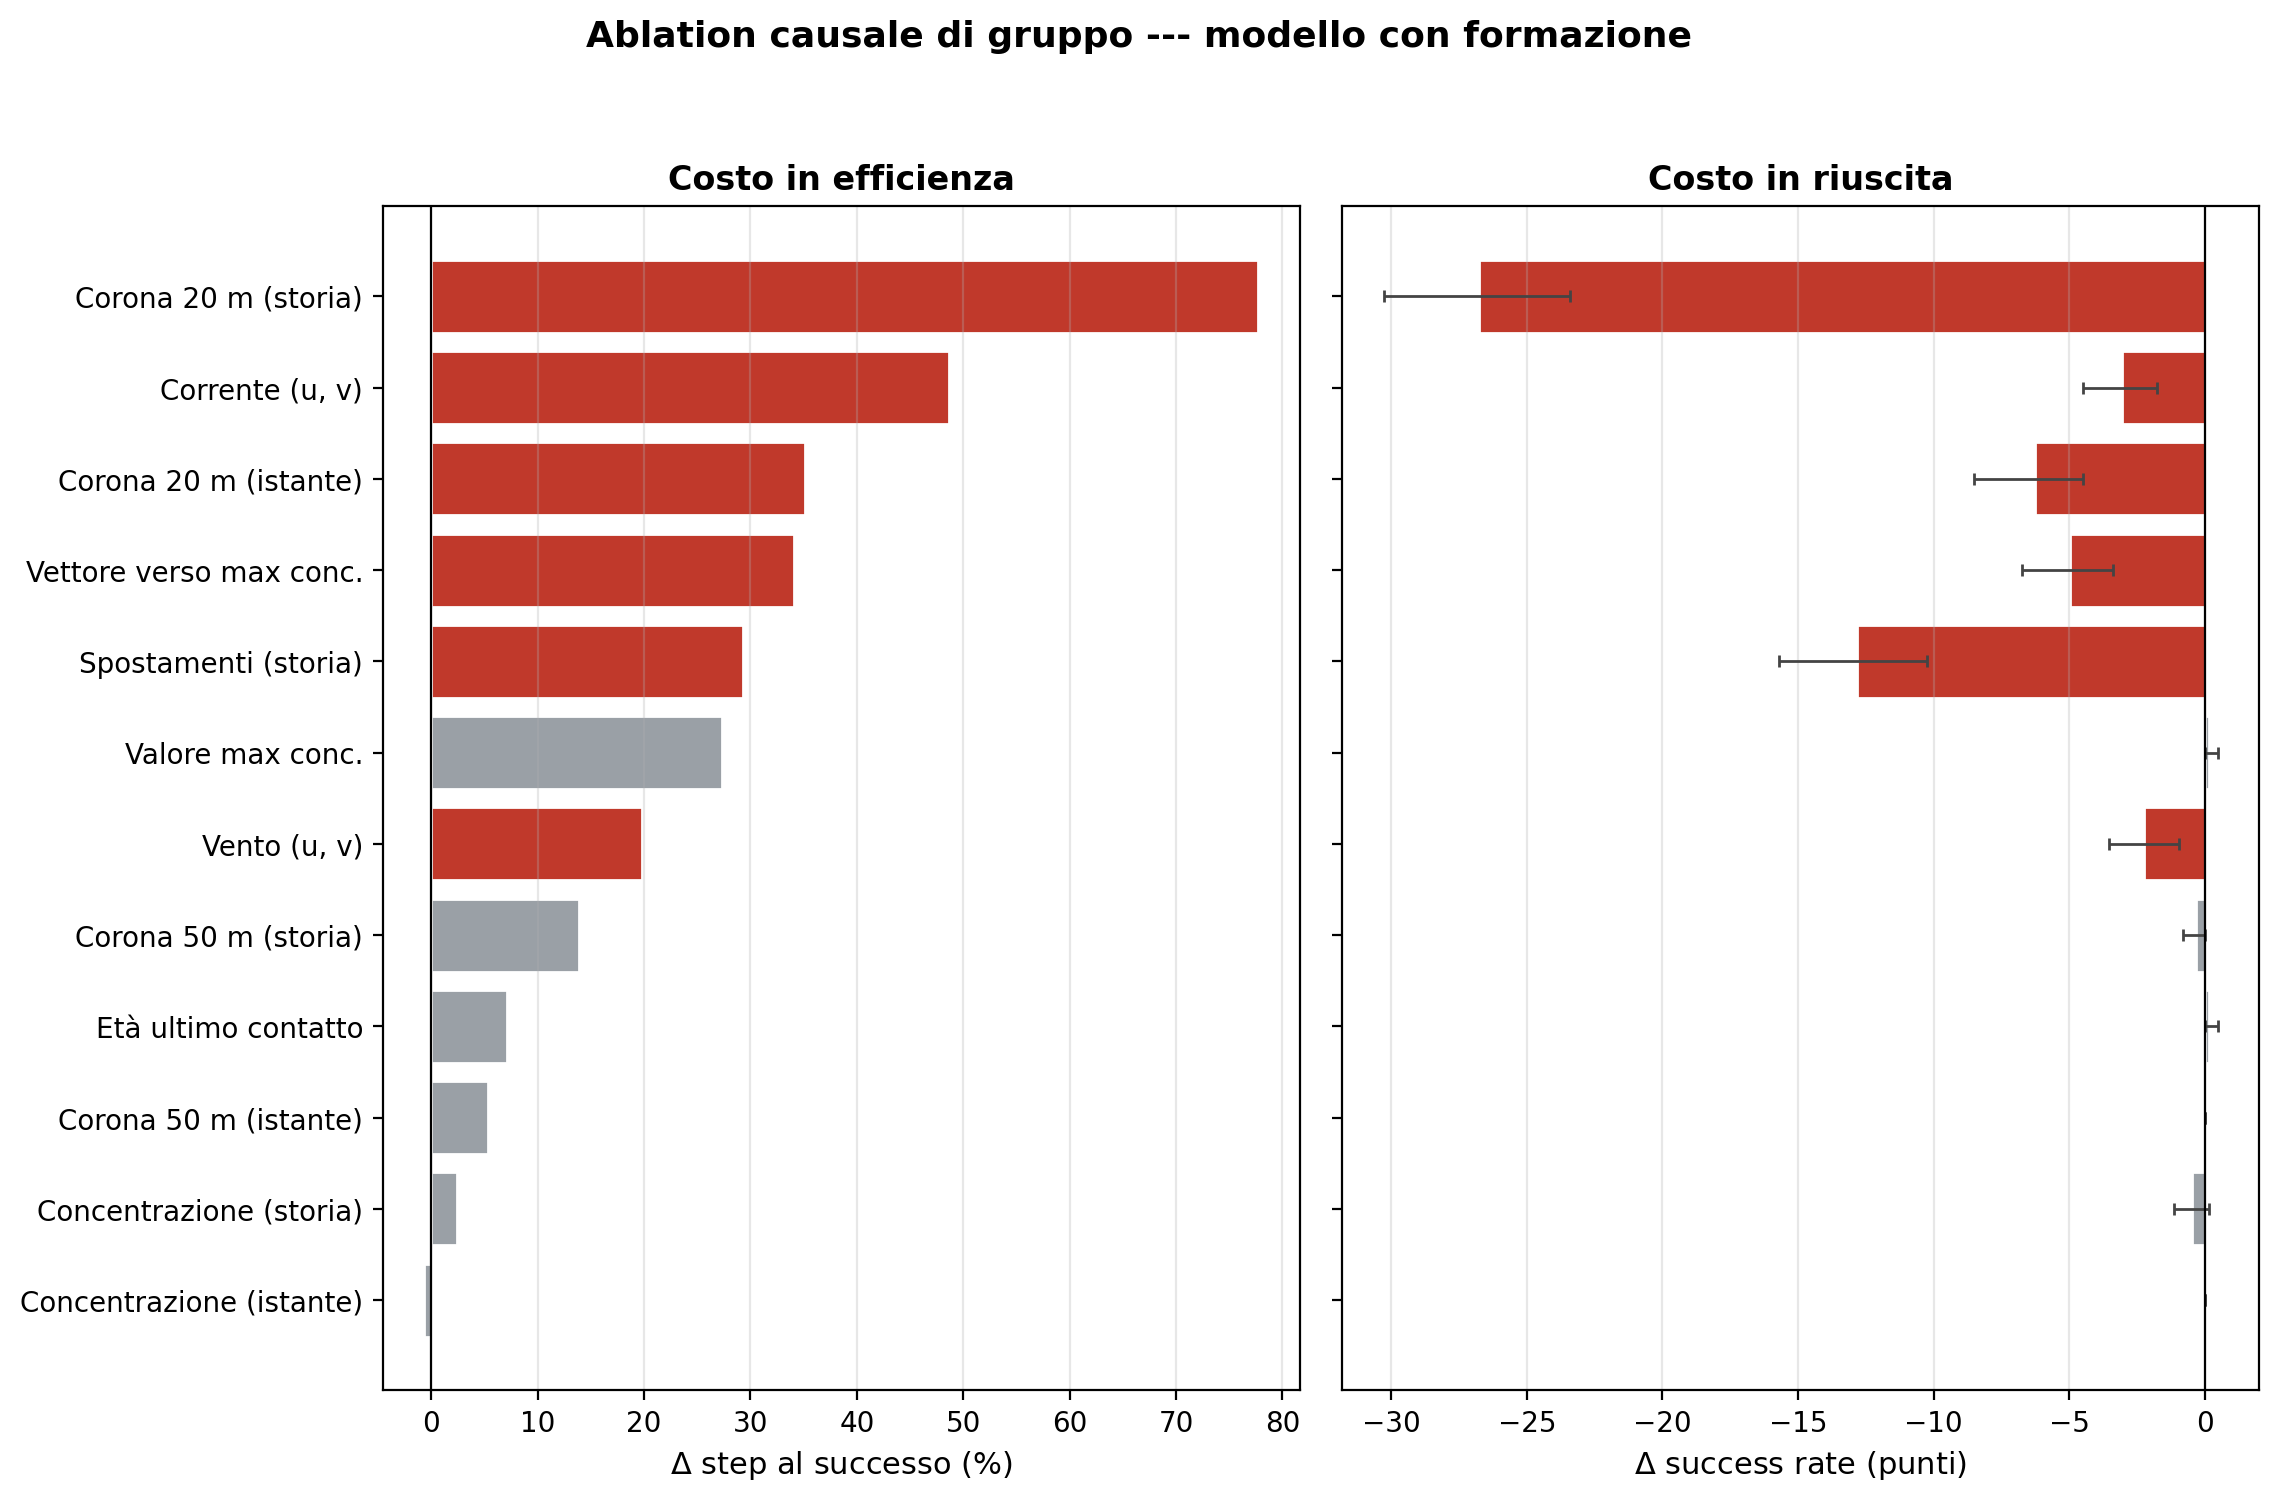
\includegraphics[width=\linewidth]{fig_ablation_clean_dualcorona.png}
  \caption{Ablation causale di gruppo sul modello a doppia corona $v_{\max}{=}2$: 624
           spawn appaiati, IC 95\% bootstrap. A sinistra il costo in efficienza (step al
           successo), a destra quello in riuscita (success rate). L'ordinamento segue
           l'efficienza. Il colore indica la \emph{classe di evidenza}: rosso se
           l'intervallo esclude lo zero, grigio se lo contiene.}
  \label{fig:xai_ablation}
\end{figure}

\paragraph{Risultati.} La baseline raggiunge il $99{,}8\%$ di success rate in $47{,}6$
step medi --- valori misurati sui 624 spawn appaiati di questo protocollo, e quindi
lievemente diversi dal $99{,}7\%$ / $49{,}8$ step riportati per lo stesso modello nella
Tabella~\ref{tab:dual_vmax} (valutazione held-out a 1560 episodi). Il risultato dominante \`e la \textbf{storia della corona a 20\,m}: rimuoverla
costa $-26{,}8$ punti di success rate (IC $[-30{,}3, -23{,}4]$) e $+77{,}7\%$ di step. \`E
di gran lunga il blocco pi\`u portante dell'intera osservazione, e il fatto che a pesare
sia la \emph{storia} --- non la lettura istantanea, che costa $-6{,}2$ punti --- dice che
la politica integra il campo chimico nel tempo anzich\'e reagire all'istante. Seguono la
memoria degli \textbf{spostamenti} ($-12{,}8$ punti), cio\`e il senso di dove si sta
andando, e il \textbf{vettore verso la massima concentrazione vista} ($-5{,}0$).

All'estremo opposto, tre gruppi risultano \textbf{indistinguibili dalla baseline} su
entrambe le metriche: la concentrazione istantanea, la sua storia e la corona a 50\,m
istantanea hanno intervalli di confidenza che contengono lo zero. Il caso della
\textbf{concentrazione istantanea} \`e il pi\`u netto: azzerarla non cambia nulla
($-0{,}7\%$ di step, IC $[-5{,}5, +4{,}5]$; success rate invariato). La lettura al centro
della formazione \`e ridondante --- gli otto sensori direzionali la circondano a
$20\,\text{m}$ e ne contengono gi\`a l'informazione --- e la politica, di fatto, la
ignora.

\paragraph{La seconda corona.} Il verdetto sulla corona a 50\,m \`e sfumato e merita
attenzione, perch\'e incrocia il risultato della Sezione~\ref{sec:rl_dual}. La sua lettura
istantanea non ha effetto misurabile ($+5{,}3\%$ di step, IC $[-0{,}4, +12{,}4]$), mentre
la sua \emph{storia} ha un effetto piccolo ma reale sull'efficienza ($+13{,}9\%$, IC
$[+7{,}0, +21{,}9]$) e nullo sulla riuscita ($-0{,}3$ punti). Il quadro \`e coerente con
il confronto per riaddestramento del Capitolo~\ref{cap:rl}, dove la doppia corona a
$v_{\max}{=}2$ risultava $28{,}3\%$ pi\`u veloce a parit\`a di success rate: i due
esperimenti --- rimuovere il sensore da un modello \emph{congelato} e riaddestrare senza
di esso --- convergono sullo stesso ordine di grandezza e sulla stessa conclusione
qualitativa, cio\`e che la seconda corona compra \textbf{velocit\`a, non affidabilit\`a}.
La convergenza di due protocolli indipendenti \`e un riscontro non banale.

\section{Valori di Shapley esatti}
\label{sec:xai_shapley}

Con dodici giocatori le $2^{12} = 4096$ coalizioni sono state enumerate integralmente su
un buffer di 1500 stati raccolti dai rollout della politica piena. Il payoff \`e
$v(S) = \pi(a^*\,|\,x_S)$, con $a^*$ l'azione scelta a osservazione completa. La media di
$\pi(a^*)$ passa da $0{,}201$ alla baseline a $0{,}707$ a osservazione piena: i dodici
gruppi si ripartiscono quindi $0{,}506$ di massa di probabilit\`a. L'assioma di
efficienza \`e verificato numericamente con un errore massimo di
$3{,}2 \times 10^{-8}$, che conferma l'esattezza del calcolo.

La Figura~\ref{fig:xai_shapley} riporta, per ciascuno dei dodici gruppi, la magnitudine media
del valore di Shapley $|\phi_i|$: la lunghezza di ogni barra misura quanto quel blocco
contribuisce, in media, alla probabilit\`a che la politica assegna all'azione scelta. \`E
quindi una graduatoria di \emph{ci\`o che la rete guarda}, ossia una lettura
\emph{osservazionale} della funzione appresa, distinta dalla \emph{necessit\`a} causale
misurata dall'ablazione (Sezione~\ref{sec:xai_ablation}); come si vedr\`a, le due letture
divergono, e il confronto \`e ripreso nella Sezione~\ref{sec:xai_sintesi}.

\begin{figure}[H]
  \centering
  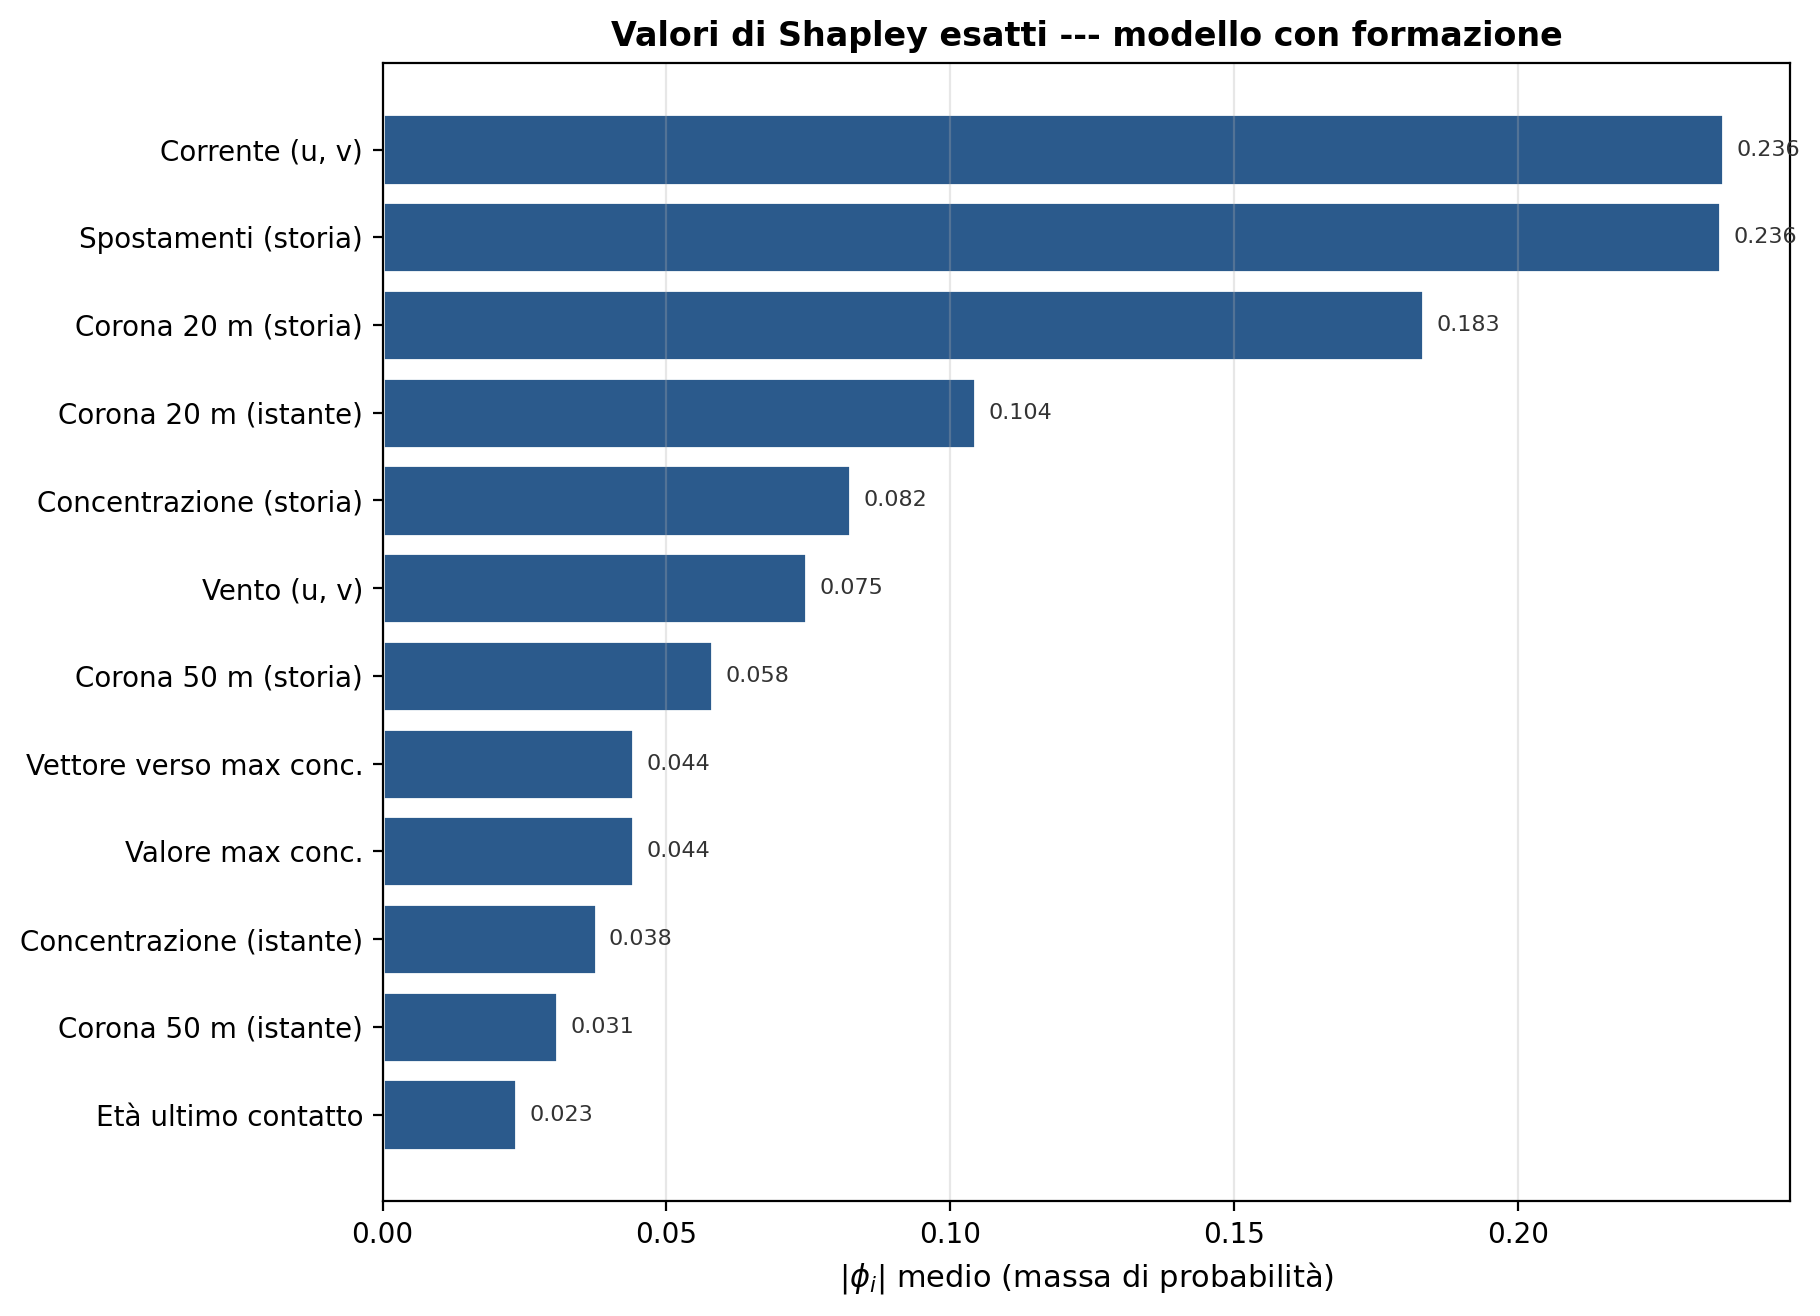
\includegraphics[width=0.94\linewidth]{fig_shapley_clean_dualcorona.png}
  \caption{Valori di Shapley esatti sui dodici gruppi: media di $|\phi_i|$ su 1500 stati,
           $4096$ coalizioni enumerate. La magnitudine \`e sull'asse, non nel colore.}
  \label{fig:xai_shapley}
\end{figure}

La graduatoria di ci\`o che la rete \emph{guarda} \`e guidata a pari merito dalla
\textbf{corrente} ($|\phi| = 0{,}236$) e dalla \textbf{memoria degli spostamenti}
($0{,}236$), seguite dalla storia della corona a 20\,m ($0{,}183$). In coda stanno l'et\`a
dell'ultimo contatto ($0{,}023$), la corona a 50\,m istantanea ($0{,}031$) e la
concentrazione istantanea ($0{,}038$).

\section{Analisi comportamentale}
\label{sec:xai_comportamento}

\paragraph{Non \`e risalita di gradiente.} La domanda pi\`u naturale su una politica di
source seeking \`e se si riduca a seguire il sensore pi\`u intenso. Per rispondere si
confronta, su 13\,738 stati con contatto col plume, la direzione del sensore massimo
della corona a 20\,m con la direzione scelta. La lettura richiede un'accortezza: gli spawn
stanno sul plume, che \`e avvettato \emph{a valle} della sorgente, quindi la sorgente cade
quasi sempre in una direzione sistematica e il marginale $P(\text{azione})$ \`e
fortemente sbilanciato. Confrontare la diagonale con $1/8$ sarebbe quindi fuorviante: va
confrontata con il valore \emph{atteso sotto indipendenza}, che incorpora quel bias.

\begin{figure}[H]
  \centering
  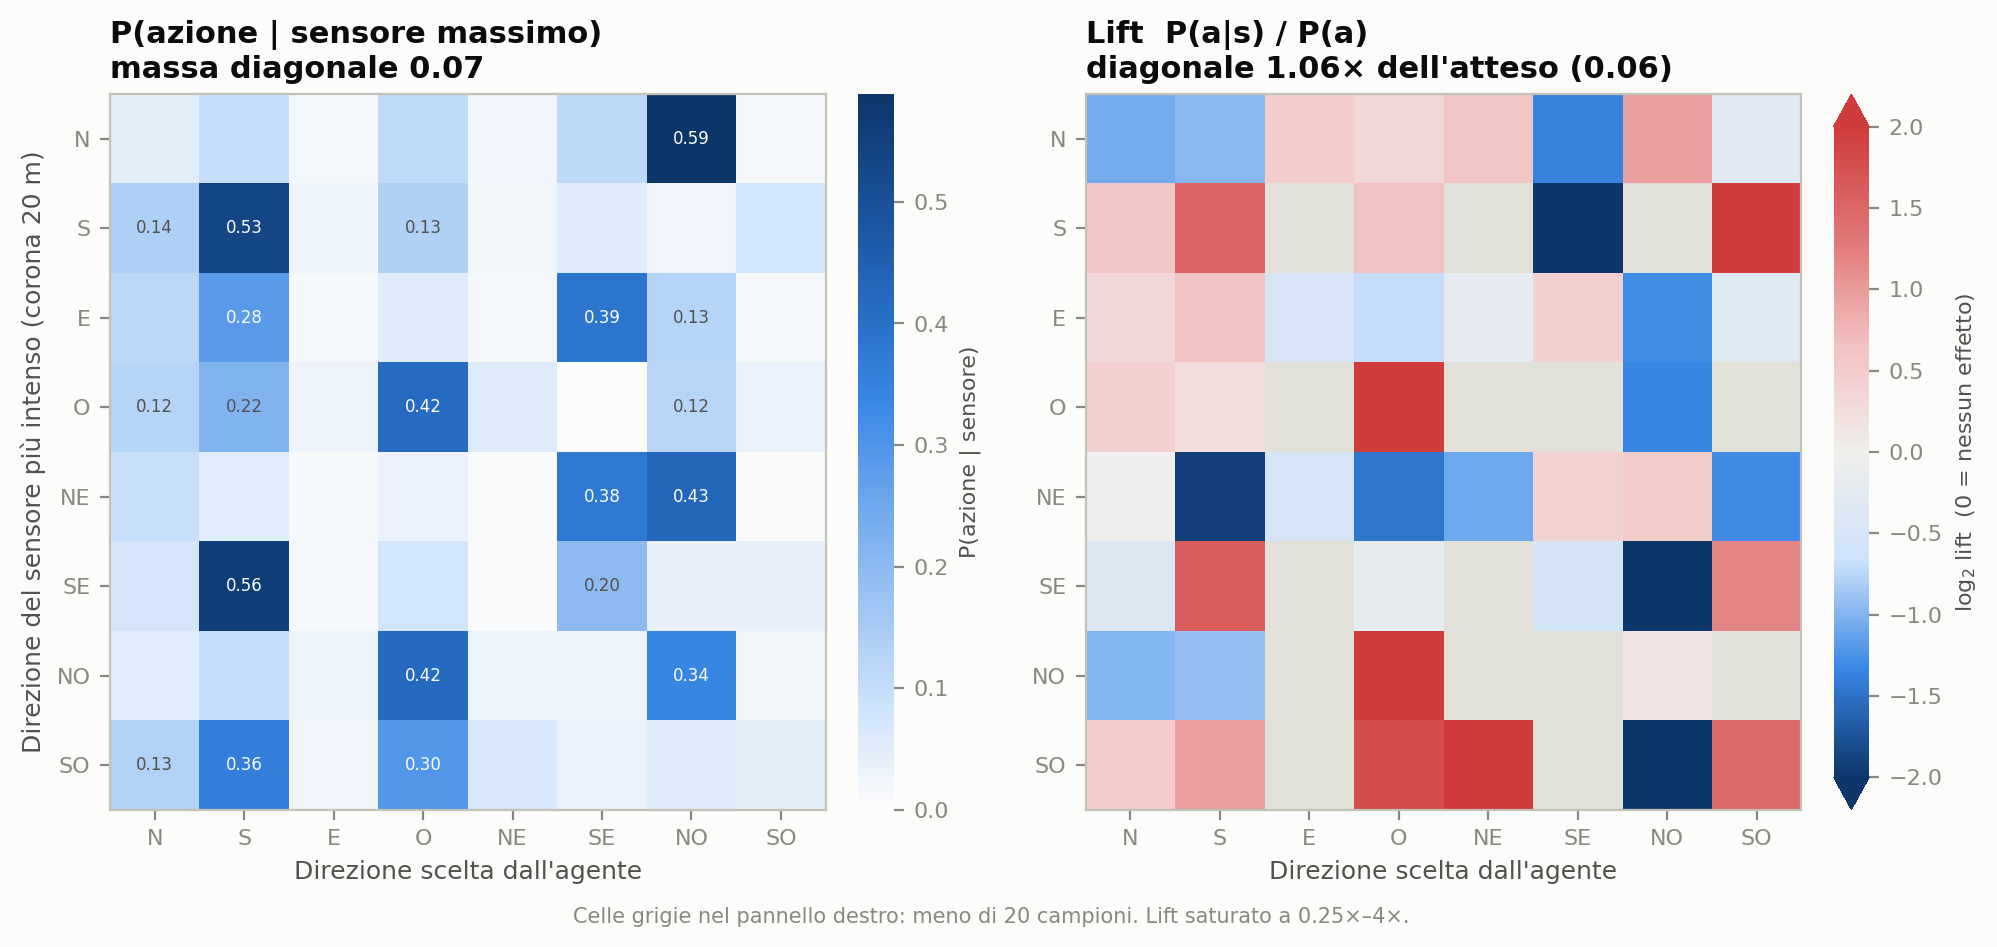
\includegraphics[width=\linewidth]{fig_sensore_azione.png}
  \caption{Sensore massimo (corona 20\,m) contro direzione scelta. A sinistra la
           condizionale $P(a|s)$, dominata dal bias direzionale degli scenari; a destra il
           \emph{lift} $P(a|s)/P(a)$, che divide per il marginale e isola il solo
           contributo del sensore ($1 = $ nessun effetto).}
  \label{fig:xai_sensore}
\end{figure}

La massa sulla diagonale \`e $0{,}068$ contro un atteso di $0{,}064$: un \textbf{lift di
appena $1{,}06\times$}. La politica muove verso il sensore pi\`u intenso solo il $6\%$
delle volte in pi\`u di quanto predica il suo stesso bias direzionale. \textbf{La politica
non fa risalita di gradiente locale}: pur essendo la corona a 20\,m il blocco pi\`u
portante dell'osservazione (Sezione~\ref{sec:xai_ablation}), non la usa per scegliere la
direzione istantanea di massima concentrazione. I due risultati non sono in
contraddizione, anzi si spiegano a vicenda: ci\`o che conta non \`e la corona ma la
\emph{sua storia}, cio\`e l'integrazione temporale del campo, esattamente la strategia che
il Capitolo~\ref{cap:rl} attribuiva all'RL per spiegare il divario con l'FCM --- il quale,
per costruzione, la risalita di gradiente locale la fa.

\paragraph{Il vento \`e letto ma non seguito.} Ruotando il vento a $360^\circ$ e tenendo
fermo il resto dell'osservazione, la direzione preferita dalla politica insegue il
controvento con un allineamento di appena $0{,}109$ (dove $1$ sarebbe anemotassi perfetta
e $0$ indifferenza). La politica, cio\`e, \textbf{non fa anemotassi}. Il dato \`e coerente
con l'addestramento: questo modello discende dalla catena \texttt{minimal}, in cui i
reward di allineamento a vento e corrente sono \emph{disattivati}
(Sezione~\ref{sec:rl_reward}) proprio perch\'e controproducenti. Il risultato vale quindi
anche come validazione del metodo: l'analisi ritrova, senza saperlo, una propriet\`a nota
del setup di addestramento.

Va segnalato il limite della sonda: ruotare il vento tenendo fermo il campo di
concentrazione produce osservazioni fuori dalla variet\`a dei dati, perch\'e vento e forma
del plume sono fisicamente accoppiati. La response curve risponde quindi alla domanda
``l'uscita della politica dipende dall'ingresso vento?'', non a ``cosa accadrebbe in un
mondo con vento diverso?''.

\paragraph{Il critic stima la distanza.} La funzione valore $V(s)$ correla negativamente
con la distanza dalla sorgente ($r = -0{,}33$ su tutti gli scenari): il critic ha appreso
una nozione di prossimit\`a senza che gliela si sia mai fornita esplicitamente. La
correlazione \`e moderata perch\'e aggregata su 26 sorgenti e 12 combinazioni
vento--chunk, ciascuna con il proprio livello di difficolt\`a: $V(s)$ stima il ritorno
atteso, che dipende anche dallo scenario, non solo dalla distanza.

\begin{figure}[H]
  \centering
  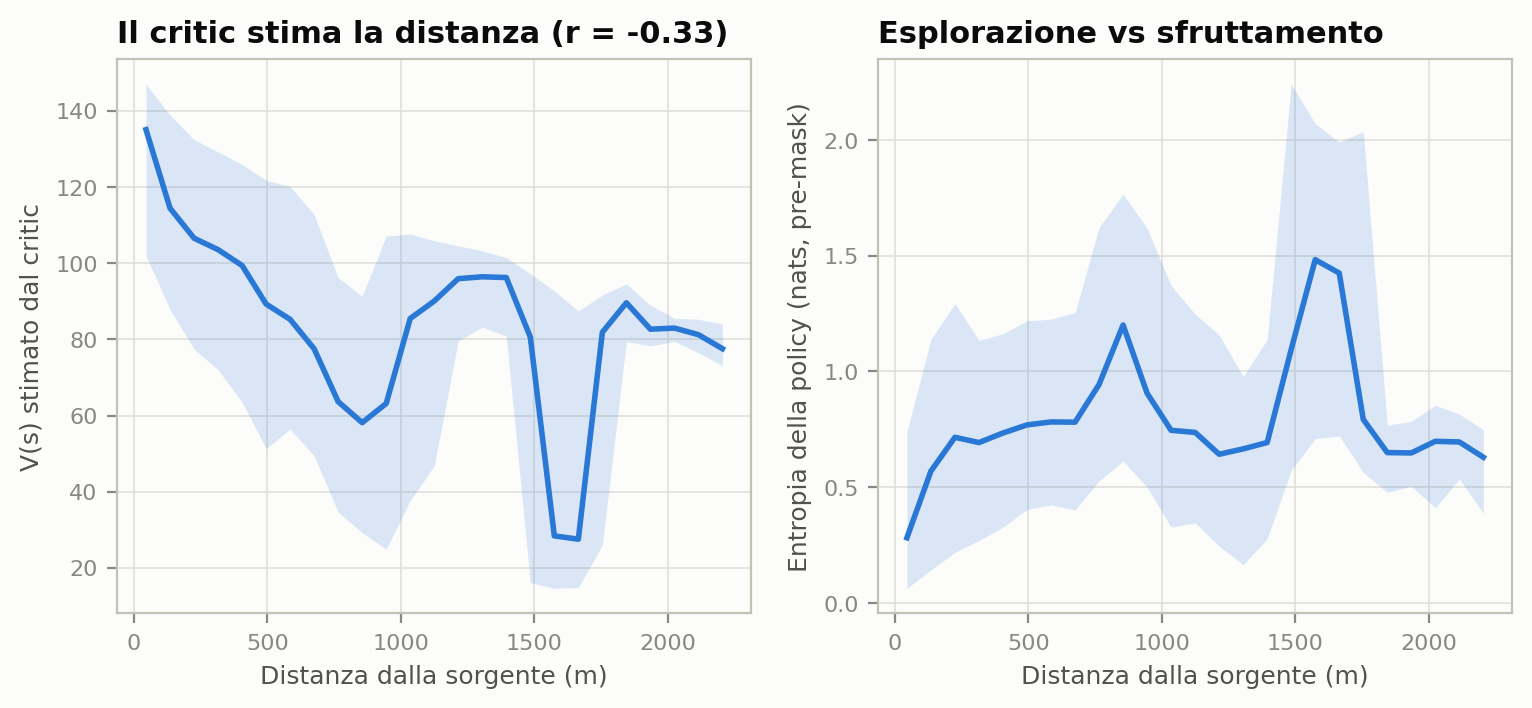
\includegraphics[width=\linewidth]{fig_valore_entropia.png}
  \caption{A sinistra $V(s)$ stimato dal critic in funzione della distanza dalla sorgente
           (mediana e intervallo interquartile per bin); a destra l'entropia della
           politica, calcolata sui logit pre-maschera.}
  \label{fig:xai_valore}
\end{figure}

\section{Il valore della formazione: ablazione per riaddestramento}
\label{sec:xai_noform}

Le ablazioni fin qui condotte operano su un modello \textbf{congelato}: si azzera un gruppo
di feature in inferenza e si misura il danno. Questo protocollo, per\`o, \emph{sovrastima}
l'importanza di una feature, perch\'e l'agente non pu\`o adattarsi alla sua assenza. Per
misurare il valore \emph{irriducibile} della formazione --- l'insieme dei sensori
direzionali che distingue la nostra squadra master--slave da un singolo veicolo --- si
adotta un protocollo pi\`u equo: \textbf{rimuovere la formazione e riaddestrare}.

\paragraph{Protocollo.} A partire dal modello a singola corona con $v_{\max}=2\,\text{m/s}$
si esegue un fine-tuning ($2$\,M step) in cui i sensori direzionali della formazione ---
correnti e storici --- sono \textbf{azzerati} ad ogni passo (\emph{masking} della
formazione). L'architettura non cambia (osservazione a 116 dimensioni, spazio d'azione
$\text{Discrete}(8\times5)$): l'agente riparte dai pesi del modello con formazione e impara
una nuova strategia con la sola informazione che gli resta --- la concentrazione nella
\emph{propria} posizione, le memorie di concentrazione e di spostamento, il vento e la
corrente. Tutto il resto (velocit\`a, protocollo held-out a 1560 episodi, dataset)
\`e identico, cos\`i che il calo di prestazioni sia attribuibile alla \emph{sola} rimozione
della formazione.

\paragraph{Costo della rimozione.} La Tabella~\ref{tab:noform_cmp} confronta l'agente
singolo con il modello a formazione di pari velocit\`a.

\begin{table}[H]
\centering
\renewcommand{\arraystretch}{1.3}
\small
\begin{tabular}{L{3.4cm} C{2.8cm} C{2.8cm} C{2.4cm}}
\toprule
\rowcolor{headerbg}
\textcolor{white}{\textbf{Metrica}} &
\textcolor{white}{\textbf{Con formazione}} &
\textcolor{white}{\textbf{Senza formazione}} &
\textcolor{white}{\textbf{$\Delta$}} \\
\midrule
\rowcolor{rowalt} \textbf{SR globale} & 99{,}7\% & \textbf{93{,}3\%} & $-6{,}4$ \\
Step medi (succ.) & 69{,}5 & 100{,}6 & $+44{,}7\%$ \\
\midrule
V0 & 100{,}0\% & 97{,}2\% & $-2{,}8$ \\
\rowcolor{rowalt} V1 & 99{,}5\% & 97{,}9\% & $-1{,}6$ \\
V2 & 99{,}2\% & 86{,}4\% & $\mathbf{-12{,}8}$ \\
\rowcolor{rowalt} V3 & 100{,}0\% & 91{,}8\% & $-8{,}2$ \\
Q1/4 & 100{,}0\% & 97{,}9\% & $-2{,}1$ \\
\rowcolor{rowalt} Q1/2 & 99{,}0\% & 90{,}0\% & $\mathbf{-9{,}0}$ \\
Q3/4 & 100{,}0\% & 92{,}1\% & $-7{,}9$ \\
\bottomrule
\end{tabular}
\caption{Modello con vs.\ senza formazione a $v_{\max}{=}2\,$m/s (1560 episodi ciascuno). Il
         $\Delta$ \`e il costo \emph{netto} della rimozione della formazione, dopo che
         l'agente ha avuto modo di adattarsi.}
\label{tab:noform_cmp}
\end{table}

La formazione vale \textbf{$6{,}4$ punti} di success rate globale e circa il $45\%$ in
velocit\`a. Il costo non \`e uniforme: \`e trascurabile negli scenari facili (V0/V1, Q1/4,
entro $-3$ punti) e diventa marcato dove il plume \`e avvettato e diffuso --- \textbf{V2}
($-12{,}8$) e \textbf{Q1/2} ($-9{,}0$) --- ossia dove il gradiente \emph{spaziale}
istantaneo delle otto letture simultanee \`e pi\`u prezioso. Il calo resta comunque
\textbf{moderato}: l'agente singolo riaddestrato recupera gran parte delle prestazioni, e
soprattutto rimane molto sopra il metodo del gradiente --- l'FCM adattivo a pari velocit\`a
($lr=20\,$m) si ferma al $58{,}2\%$, circa \textbf{35 punti} sotto l'agente singolo (93{,}3\%).
\`E un fatto notevole: un agente RL che vede solo la propria concentrazione batte nettamente
un metodo reattivo che dispone dell'intera formazione. Ci\`o che separa il successo dal
fallimento non \`e il sensore, ma la strategia appresa.

\paragraph{Come compensa l'agente singolo.} L'explainability del modello senza formazione
(stesso protocollo: ablazione di gruppo e Shapley esatti) rivela uno \textbf{spostamento del
baricentro informativo dal sensing spaziale a quello temporale}
(Tabella~\ref{tab:noform_shift}, Figura~\ref{fig:noform_xai}). Privato della corona,
l'agente si regge in modo schiacciante sulla \textbf{memoria degli spostamenti} (ablazione
$-55{,}6$ punti, Shapley $|\phi|=0{,}27$): correla i propri movimenti con le variazioni
della concentrazione che misura sotto di s\'e, ricostruendo nel \emph{tempo} il gradiente
che la formazione forniva nello \emph{spazio}. Seguono l'\emph{homing} verso la massima
concentrazione vista ($-25{,}8$), la corrente ($-12{,}8$) e la storia della concentrazione
propria ($-11{,}2$) --- proprio la feature che il modello \emph{con} formazione ignorava
($\approx 0$).

Come per il modello con formazione (Sezione~\ref{sec:xai_sintesi}), anche qui
\emph{attribuzione} e \emph{necessit\`a} divergono, e nello stesso modo istruttivo. Il
\textbf{vettore verso il massimo di concentrazione} \`e solo quarto per attribuzione
($|\phi| = 0{,}07$) ma \textbf{secondo per impatto causale} ($-25{,}8$): l'homing di memoria
\`e insostituibile per il compito pur essendo poco ``guardato'' dalla rete. Specularmente, la
\textbf{corrente} \`e seconda per attribuzione ($|\phi| = 0{,}12$) ma pesa meno all'ablazione
($-12{,}8$), confermando --- ora anche in assenza della corona --- che ci\`o che la rete
osserva non coincide con ci\`o che le \`e strettamente necessario.

\begin{table}[H]
\centering
\renewcommand{\arraystretch}{1.3}
\small
\begin{tabular}{L{5.4cm} C{2.9cm} C{2.9cm}}
\toprule
\rowcolor{headerbg}
\textcolor{white}{\textbf{Gruppo ($\Delta$SR)}} &
\textcolor{white}{\textbf{Con formazione}} &
\textcolor{white}{\textbf{Senza formazione}} \\
\midrule
Corona 20\,m (storia)              & $\mathbf{-26{,}8}$ & mascherata \\
\rowcolor{rowalt} Spostamenti (storia) & $-12{,}8$ & $\mathbf{-55{,}6}$ \\
Corona 20\,m (istante)             & $-6{,}2$  & mascherata \\
\rowcolor{rowalt} Vettore verso max conc.\ (homing) & $-5{,}0$ & $-25{,}8$ \\
Corrente $(u,v)$                   & $-3{,}0$  & $-12{,}8$ \\
\rowcolor{rowalt} Vento $(u,v)$    & $-2{,}2$  & $-1{,}4$ \\
Concentrazione (storia)            & $-0{,}5$  & $-11{,}2$ \\
\rowcolor{rowalt} Corona 50\,m (storia) & $-0{,}3$ & --- \\
Concentrazione (istante)           & $0{,}0$   & $-3{,}2$ \\
\rowcolor{rowalt} Corona 50\,m (istante) & $0{,}0$ & --- \\
Valore max conc.                   & $+0{,}2$  & $-7{,}1$ \\
\rowcolor{rowalt} Et\`a ultimo contatto & $+0{,}2$ & $-0{,}5$ \\
\bottomrule
\end{tabular}
\caption{Spostamento del baricentro informativo: costo in success rate ($\Delta$SR,
         punti percentuali) di \emph{ogni} gruppo, per il modello \emph{con} formazione
         (doppia corona, ablazioni della Sezione~\ref{sec:xai_ablation}) e per l'agente
         \emph{senza} formazione (singola corona, formazione mascherata). Con la formazione la
         politica si regge sul gradiente \emph{spaziale} (storia della corona); rimossa, il
         peso si trasferisce sul sensing \emph{temporale} --- spostamenti, homing, storia e
         valore di concentrazione, tutti nettamente pi\`u costosi. ``mascherata'': corona
         azzerata, effetto spurio escluso (Figura~\ref{fig:noform_xai}); ``---'': gruppo
         assente, poich\'e l'agente singolo ha una sola corona.}
\label{tab:noform_shift}
\end{table}

\begin{figure}[H]
  \centering
  \begin{subfigure}{\linewidth}
    \centering
    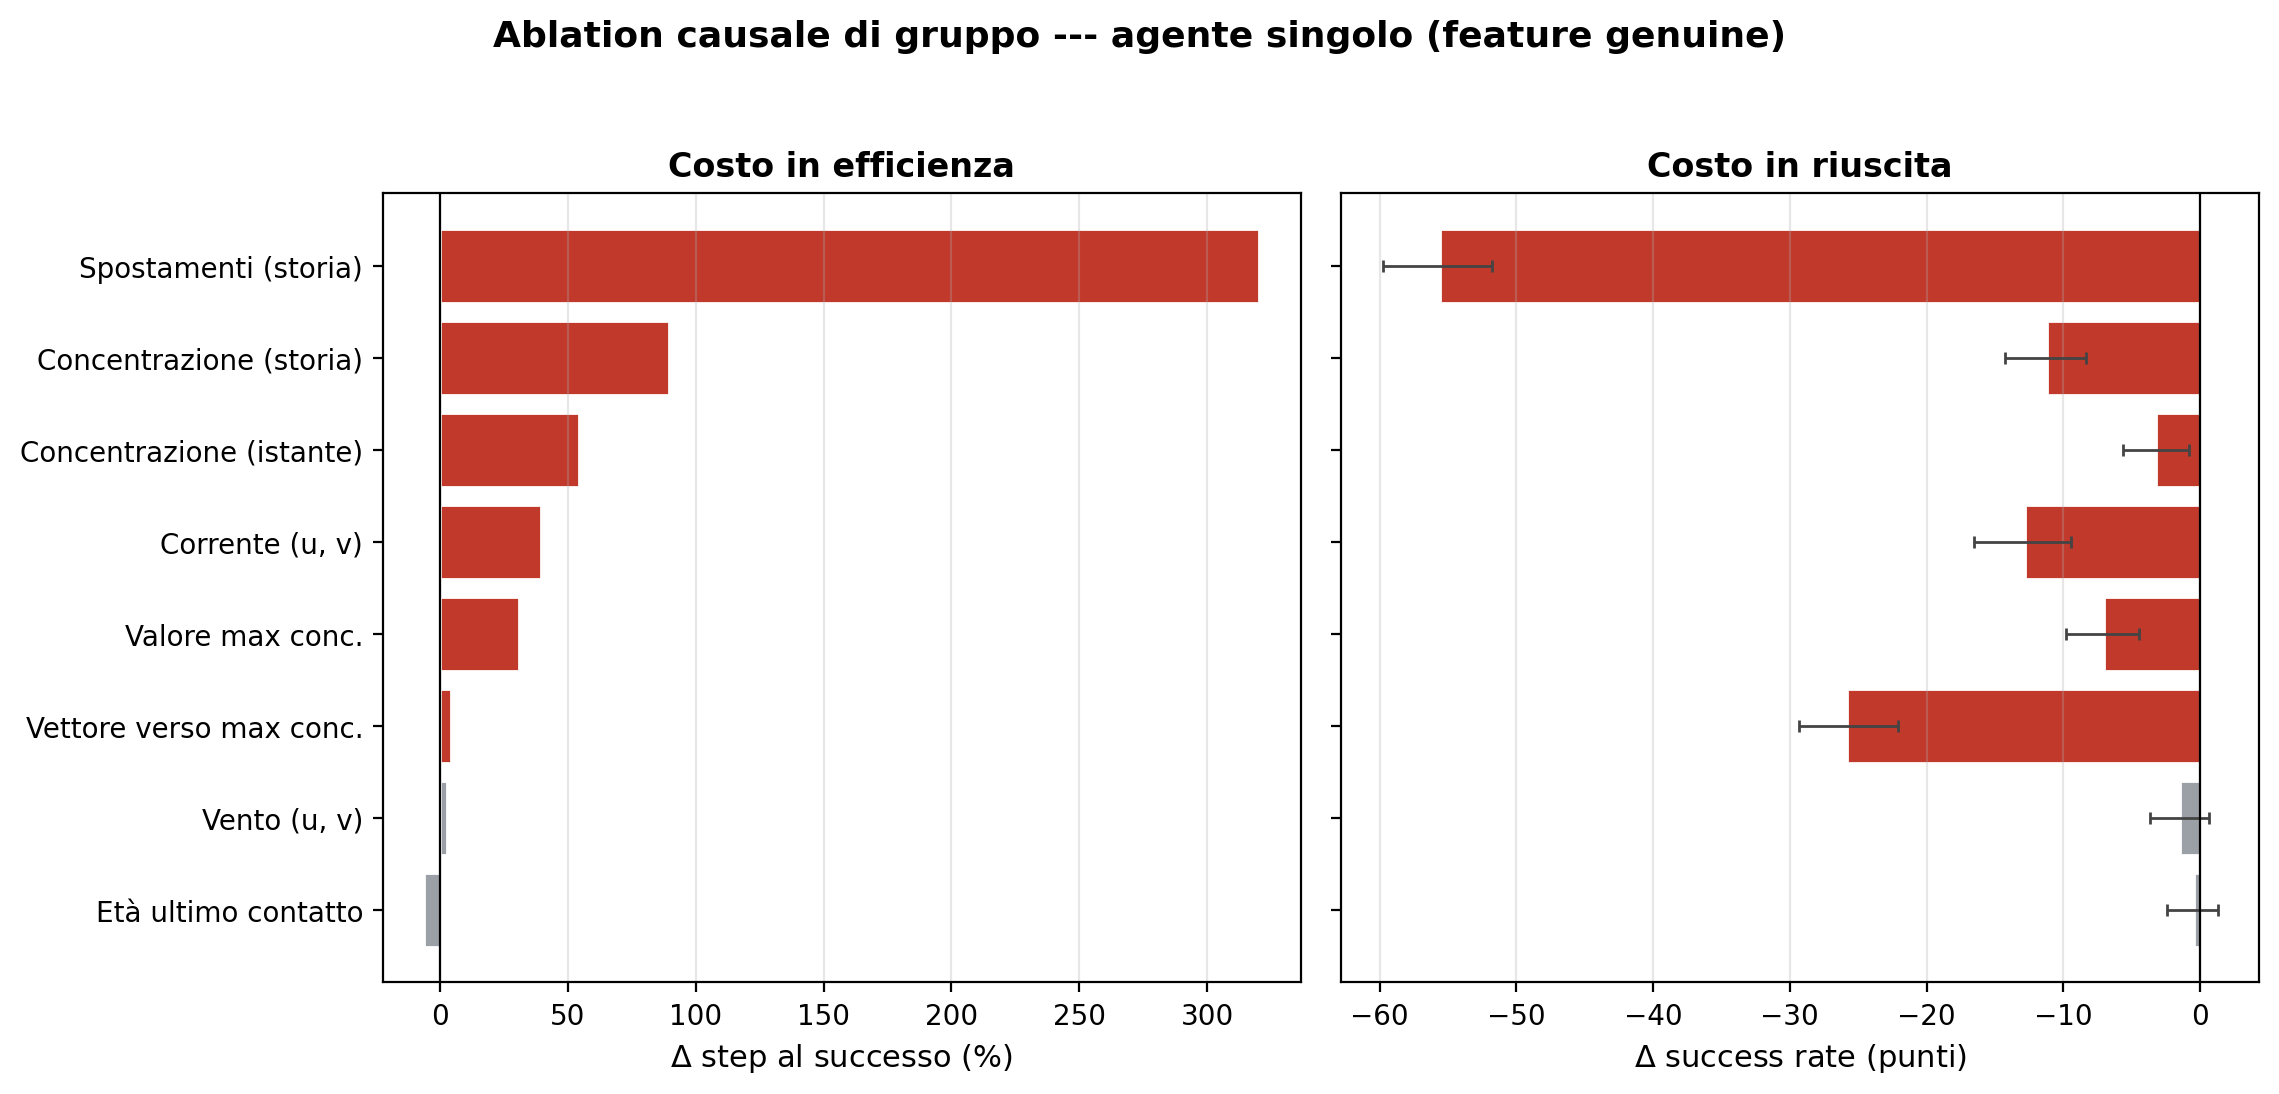
\includegraphics[width=\linewidth]{fig_ablation_clean_noformation.png}
    \caption{Ablazione di gruppo.}
  \end{subfigure}

  \vspace{5mm}
  \begin{subfigure}{\linewidth}
    \centering
    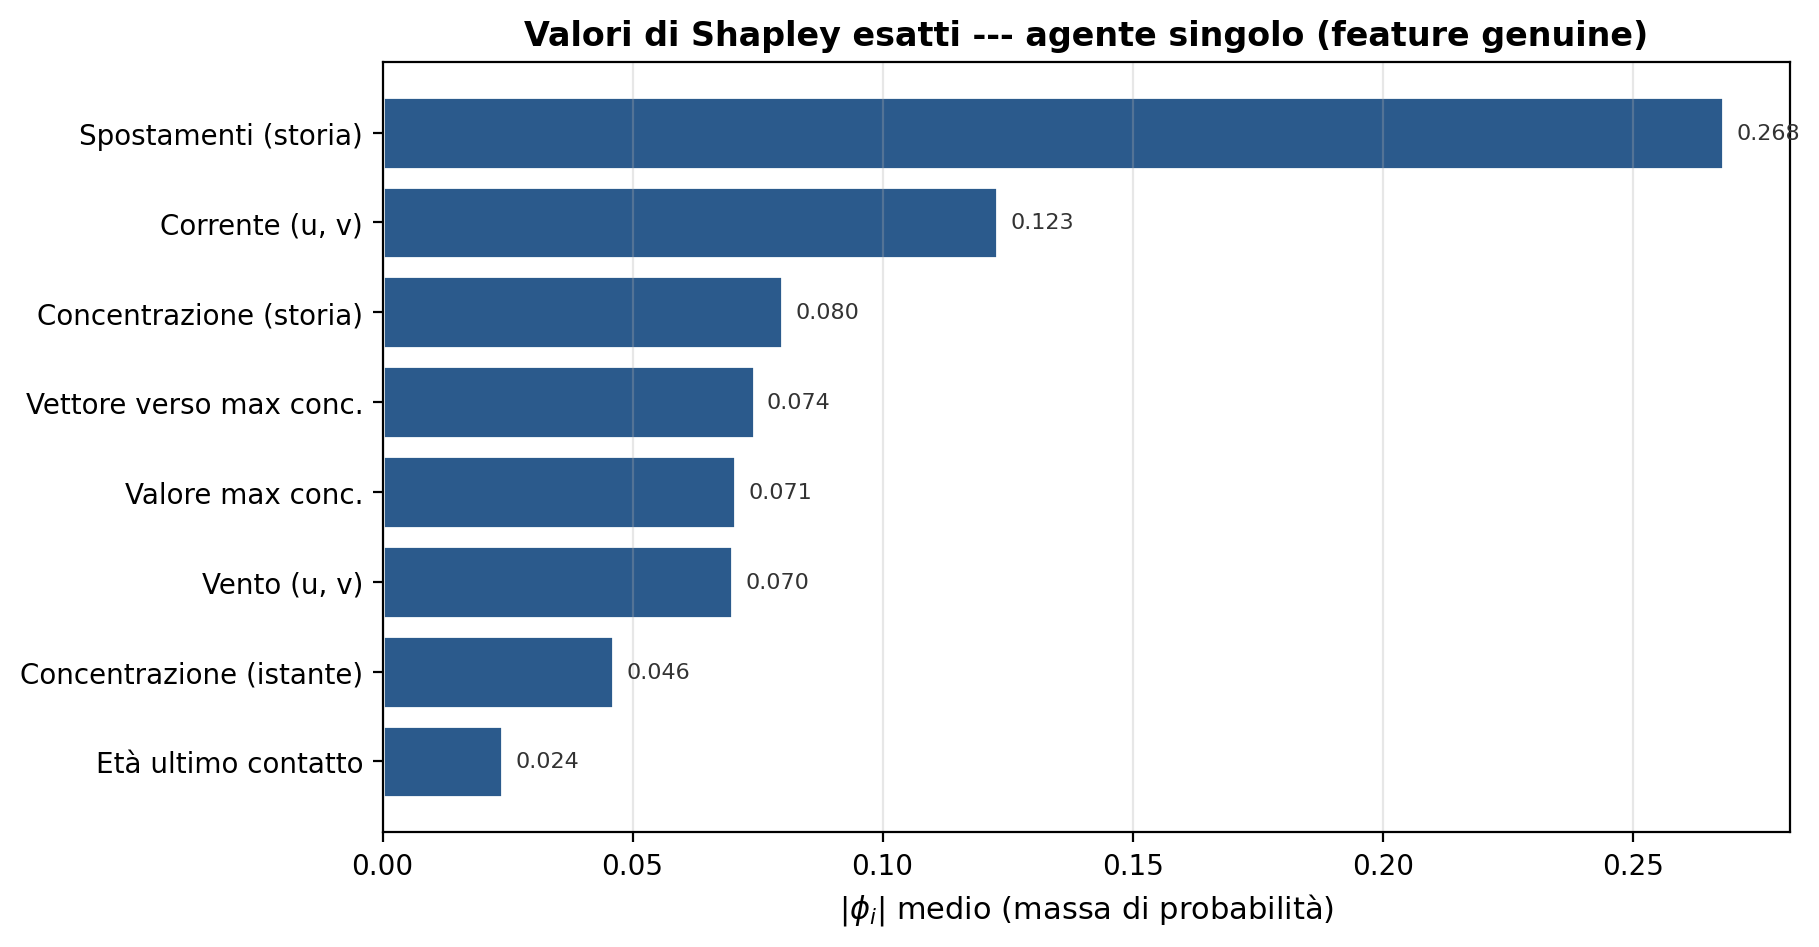
\includegraphics[width=0.9\linewidth]{fig_shapley_clean_noformation.png}
    \caption{Valori di Shapley esatti.}
  \end{subfigure}
  \caption{Explainability dell'agente singolo (senza formazione), sui soli gruppi
           \emph{genuini}: la memoria degli spostamenti \`e la feature portante, seguita
           dall'homing verso il massimo di concentrazione e dalla corrente. I gruppi della
           corona sono \textbf{esclusi} perch\'e mascherati a zero: \texttt{VecNormalize} li
           rende una costante non nulla il cui azzeramento perturberebbe il bias appreso,
           producendo un effetto spurio privo di contenuto informativo.}
  \label{fig:noform_xai}
\end{figure}

Il quadro chiude il cerchio dell'analisi: la rete non ``perde un pezzo'' quando le si toglie
la formazione, ma \textbf{ricompone} la stima della direzione con gli strumenti che le
restano. La formazione \`e un vantaggio reale ma \emph{sostituibile in parte} da una
strategia temporale appresa; \`e negli scenari a plume diffuso, dove il segnale temporale
degenera pi\`u in fretta, che il suo contributo spaziale resta insostituibile.

\section{Sintesi: che cosa la rete guarda, che cosa le serve}
\label{sec:xai_sintesi}

Il confronto fra le due graduatorie \`e la parte pi\`u istruttiva del capitolo, perch\'e
\textbf{divergono}.

\begin{table}[H]
\centering
\renewcommand{\arraystretch}{1.3}
\small
\begin{tabular}{L{4.1cm} C{2.2cm} C{1.9cm} L{3.9cm}}
\toprule
\rowcolor{headerbg}
\textcolor{white}{\textbf{Gruppo}} &
\textcolor{white}{\textbf{Shapley $|\phi|$}} &
\textcolor{white}{\textbf{$\Delta$SR}} &
\textcolor{white}{\textbf{Lettura}} \\
\midrule
Corona 20\,m (storia)          & 0{,}183 (3\textsuperscript{o})  & $\mathbf{-26{,}8}$ & indispensabile \\
\rowcolor{rowalt}
Spostamenti (storia)           & 0{,}236 (1\textsuperscript{o})  & $-12{,}8$ & indispensabile \\
Corona 20\,m (istante)         & 0{,}104 (4\textsuperscript{o})  & $-6{,}2$  & necessaria \\
\rowcolor{rowalt}
Vettore verso max conc.\ (homing) & 0{,}044 (8\textsuperscript{o}) & $-5{,}0$ & necessaria, poco guardata \\
Corrente $(u,v)$               & \textbf{0{,}236} (1\textsuperscript{o}) & $-3{,}0$ & guardata, poco necessaria \\
\rowcolor{rowalt}
Vento $(u,v)$                  & 0{,}075 (6\textsuperscript{o})  & $-2{,}2$  & guardata, poco necessaria \\
Concentrazione (storia)        & 0{,}082 (5\textsuperscript{o})  & $-0{,}5$  & guardata, poco necessaria \\
\rowcolor{rowalt}
Corona 50\,m (storia)          & 0{,}058 (7\textsuperscript{o})  & $-0{,}3$  & ridondante \\
Concentrazione (istante)       & 0{,}038 (10\textsuperscript{o}) & $0{,}0$   & ridondante \\
\rowcolor{rowalt}
Corona 50\,m (istante)         & 0{,}031 (11\textsuperscript{o}) & $0{,}0$   & ridondante \\
Valore max conc.               & 0{,}044 (8\textsuperscript{o})  & $+0{,}2$  & ridondante \\
\rowcolor{rowalt}
Et\`a ultimo contatto          & 0{,}023 (12\textsuperscript{o}) & $+0{,}2$  & ridondante \\
\bottomrule
\end{tabular}
\caption{Attribuzione (Shapley $|\phi|$: \emph{che cosa la rete guarda}) contro necessit\`a
         causale (ablation $\Delta$SR in punti percentuali: \emph{che cosa serve al compito}),
         per tutti i dodici gruppi, ordinati per necessit\`a decrescente. Le due graduatorie
         \textbf{divergono}: la \emph{corrente} \`e la pi\`u guardata (Shapley 1\textsuperscript{o})
         ma poco necessaria ($-3{,}0$), mentre la \emph{storia della corona} \`e solo terza per
         attribuzione ma di gran lunga la pi\`u necessaria ($-26{,}8$); specularmente l'\emph{homing}
         \`e poco guardato (8\textsuperscript{o}) ma utile ($-5{,}0$).}
\label{tab:xai_sintesi}
\end{table}

Il caso pi\`u istruttivo \`e la \textbf{corrente marina}: \`e il gruppo con
l'attribuzione pi\`u alta in assoluto ($|\phi| = 0{,}236$, primo a pari merito), eppure
rimuoverla costa appena $3$ punti di success rate. La rete la legge molto, ma il compito
ne ha poco bisogno --- segno che l'informazione che la corrente veicola \`e in larga parte
\emph{recuperabile} dagli altri blocchi, in primo luogo dalla storia della corona, che del
trasporto porta gi\`a la traccia. Simmetricamente, la \textbf{storia della corona a
20\,m} \`e solo terza per attribuzione ma prima, e di gran lunga, per impatto causale: \`e
l'unico blocco davvero non sostituibile.

\`E precisamente la divergenza che giustifica l'impianto metodologico della
Sezione~\ref{sec:xai_rassegna}. Un capitolo fondato sui soli metodi post-hoc avrebbe
concluso che la corrente \`e la grandezza pi\`u importante per la politica; l'intervento
mostra che, se la si toglie, la politica se la cava quasi altrettanto bene. Le due
domande --- che cosa la rete guarda, che cosa serve al compito --- hanno risposte diverse,
e solo la seconda \`e quella che conta per decidere quali sensori montare a bordo.

Ne emerge un ritratto coerente della politica appresa. Essa \textbf{non} \`e un
risalitore di gradiente: la direzione istantanea di massima concentrazione non guida la
scelta (lift $1{,}06\times$), e la concentrazione al centro della formazione \`e
addirittura ignorata. Ci\`o su cui si regge \`e l'\textbf{integrazione temporale} del
campo chimico locale --- la storia della corona a 20\,m, il blocco pi\`u portante, unita
alla memoria di dove si \`e andati --- affiancata da una memoria esplicita del punto
migliore incontrato. La seconda corona a 50\,m serve a puntare meglio le falcate lunghe,
comprando velocit\`a e non affidabilit\`a, in accordo con quanto il
Capitolo~\ref{cap:rl} aveva stabilito per riaddestramento. Vento e corrente vengono letti
ma non usati come bussola. \`E, in sintesi, esattamente la strategia che il
Capitolo~\ref{cap:rl} ipotizzava per spiegare il divario con il metodo del gradiente ---
con la differenza che qui \`e misurata anzich\'e supposta.
  % Cap. 6 --- Explainability della politica appresa
\chapter{Conclusioni}
\label{cap:concl}

Questa tesi ha affrontato il problema del \emph{source seeking} marino --- la
localizzazione autonoma della sorgente di un inquinante a partire dalle letture locali
di concentrazione --- confrontando due famiglie di approcci nell'ambito del progetto
HYDRAS, su un dataset di simulazioni idrodinamiche realistiche della baia di Cecina.

\section{Risultati principali}

Ripercorriamo il cammino della tesi dall'inizio alla fine, raccogliendone i risultati
salienti.

\paragraph{Il problema e i dati.}
Il punto di partenza \`e un problema concreto: localizzare in modo autonomo la sorgente di
uno sversamento inquinante dalle sole letture locali di concentrazione, in un ambiente
costiero dove la dispersione \`e governata da una dinamica complessa di correnti, vento e
turbolenza. Nell'ambito del progetto HYDRAS, il compito \`e stato affrontato su un dataset
di simulazioni idrodinamiche ad alta risoluzione (MIKE21) della baia di Cecina
(Capitolo~\ref{cap:dati}), forzate dai dati meteo-oceanografici di CMEMS ed ERA5: 132
sorgenti equispaziate, ciascuna simulata sotto quattro scenari di vento (V0--V3) che
generano plume dalle morfologie marcatamente diverse. Per una valutazione rigorosa, 26
sorgenti (SRC107--132) sono state riservate alla sola inferenza --- mai viste in
addestramento --- e ogni simulazione \`e stata suddivisa in tre finestre temporali,
definendo il protocollo \emph{held-out} su cui entrambi gli approcci sono stati misurati a
parit\`a di condizioni.

\paragraph{L'ambiente condiviso.}
Su questi dati \`e stato costruito un unico ambiente di simulazione
(Capitolo~\ref{cap:ambiente}), condiviso dai due approcci: una squadra \emph{master--slave}
in cui un agente master decide il movimento e otto slave, disposti in corona lungo le
direzioni cardinali e diagonali, campionano la concentrazione e gliela riportano. L'ambiente
definisce lo spazio d'azione discreto, l'\emph{action masking} che impedisce le collisioni
con la costa, la procedura di inizializzazione sul plume e un segnale di reward. Far operare
i due metodi sullo stesso ambiente --- stessa dinamica, stessi vincoli, stesse osservazioni
--- \`e ci\`o che rende il confronto pulito: l'unica variabile \`e il modulo che, ricevuta
l'osservazione, sceglie l'azione.

\paragraph{Il metodo del gradiente.}
Il primo modulo \`e il \textbf{Field Climbing Method} (Capitolo~\ref{cap:fcm}), la baseline
gradient-based. Nella versione a passo fisso raggiunge un success rate globale di appena il
\textbf{32{,}9\%}, limitato dalla sua natura puramente reattiva. L'introduzione
dell'ottimizzatore \textbf{Adam} per il calcolo del passo --- con momentum sul gradiente
stimato e normalizzazione per la varianza storica --- lo porta fino al \textbf{63{,}5\%}
($lr = 40\,\text{m}$), con un guadagno di oltre trenta punti: il momentum smorza le
oscillazioni dovute al rumore del sensore. Il passo ottimale non \`e per\`o il pi\`u ampio
--- oltre i $40\,\text{m}$ falcate troppo lunghe scavalcano la struttura del plume --- e i
valori pi\`u performanti implicano velocit\`a superiori a quella nominale del veicolo. Al di
l\`a di questi affinamenti, il limite resta \emph{strutturale}: negli scenari a plume diffuso
il gradiente locale degenera e il metodo, privo di memoria e di contesto, si blocca.

\paragraph{L'apprendimento per rinforzo.}
Il secondo modulo \`e un agente addestrato con \textbf{PPO} (Capitolo~\ref{cap:rl}). Uno
studio di ablation sulla funzione di reward ha mostrato che la variante pi\`u semplice
(\texttt{minimal}), basata sul solo gradiente chimico come segnale direzionale, ottiene il
success rate pi\`u alto (\textbf{96{,}9\%}): i reward di allineamento a vento e corrente si
sono rivelati addirittura controproducenti, perch\'e fondati sull'ipotesi --- non valida in
ambiente costiero --- di una sorgente sempre controvento. Rendere poi la \textbf{velocit\`a
una scelta dell'agente} (spazio $\text{Discrete}(8\times5)$, addestrato a catena alzando
progressivamente $v_{\max}$) ha portato il success rate al \textbf{$99{,}7$--$99{,}9\%$} e
ridotto di oltre quattro volte il tempo al successo (da $\sim$20 a $\sim$5 minuti simulati).
Su questa catena, la \textbf{doppia corona} di sensori si \`e rivelata un vantaggio netto a
partire da $v_{\max} = 2\,\text{m/s}$ --- stessa affidabilit\`a e $25$--$34\%$ di passi in
meno --- correggendo la lettura di un primo confronto in cui, addestrata da zero, sembrava
dannosa. Approfondimenti mirati hanno infine mostrato che l'agente sa \emph{manovrare}
finemente attorno alla sorgente (test a raggio di successo ridotto) e che l'esito di un
episodio \textbf{non dipende dalla posizione di partenza} (analisi delle \emph{spawn map}),
ma solo dalle condizioni idrodinamiche dello scenario.

\paragraph{Il confronto.}
Il confronto diretto \`e netto: il modello RL supera il metodo del gradiente su ogni scenario.
Poich\'e entrambi dispongono di una versione a velocit\`a variabile, il confronto pi\`u equo
\`e quello \textbf{a parit\`a di velocit\`a massima}, che neutralizza il vantaggio cinematico
di un passo pi\`u lungo: a ogni livello di velocit\`a il PPO domina l'FCM di
\textbf{$36$--$42$ punti} di success rate, con il divario massimo proprio negli scenari a
plume diffuso, dove il gradiente locale degenera. Esteso all'intero range operativo (da
$0{,}1$ a $5\,\text{m/s}$), il quadro non cambia: il PPO supera il $98\%$ gi\`a a
$1{,}2\,\text{m/s}$ e si stabilizza attorno al $99\%$, mentre l'FCM resta confinato attorno al
$55$--$63\%$ alle velocit\`a operative; l'unico regime in cui il divario si assottiglia \`e
quello delle velocit\`a pi\`u basse, dove un deficit puramente fisico di propulsione --- il
veicolo pi\`u lento delle correnti da risalire --- penalizza ogni strategia.

\paragraph{L'interpretazione della politica.}
Stabilito \emph{che} la politica funziona, il Capitolo~\ref{cap:xai} ne ha indagato il
\emph{perch\'e}. Tramite ablation causale di gruppo, valori di Shapley esatti e sonde
comportamentali \`e emerso un ritratto coerente: la politica \textbf{non} \`e un risalitore di
gradiente locale (muove verso il sensore pi\`u intenso solo il $6\%$ delle volte in pi\`u di
quanto predica il suo stesso bias direzionale), ma si regge sull'\textbf{integrazione
temporale} del campo chimico --- la storia della corona di sensori --- unita alla memoria di
dove si \`e andati. \`E emersa inoltre una divergenza istruttiva fra \emph{ci\`o che la rete
guarda} e \emph{ci\`o che le serve}: la corrente marina \`e la grandezza pi\`u ``guardata''
eppure la sua rimozione costa pochissimo, mentre la storia della corona \`e il solo blocco
davvero insostituibile. Un esperimento di riaddestramento \emph{senza} formazione ne ha
infine quantificato il valore: la formazione vale circa \textbf{$6{,}4$ punti} di success
rate, ma \`e in parte sostituibile da una strategia temporale appresa --- l'agente singolo
riaddestrato resta al $93{,}3\%$, circa trentacinque punti sopra l'FCM che pure dispone
dell'intera formazione. Ci\`o che separa il successo dal fallimento, in definitiva, non \`e il
sensore ma la \textbf{strategia appresa}.

\section{Sviluppi futuri}

La direzione di sviluppo pi\`u naturale e ambiziosa \`e il passaggio da un sistema a
\emph{singolo decisore} a un \textbf{sistema multi-agente cooperativo ``vero''}.
Nell'architettura master--slave adottata in questa tesi un solo agente (il master) decide
il movimento, mentre gli otto slave sono sensori passivi in formazione rigida: di fatto il
problema resta a singolo agente. La visione complessiva del progetto HYDRAS prevede invece
una squadra di $n$ robot autonomi, ciascuno dotato di una \emph{propria} politica di
navigazione, che collaborano --- coordinando l'esplorazione, ripartendosi il dominio e
scambiandosi informazioni --- per localizzare la sorgente pi\`u rapidamente e con maggiore
robustezza di un sistema centralizzato.

\paragraph{L'algoritmo MAPPO.} Per addestrare una tale squadra, l'estensione naturale del
PPO impiegato in questa tesi \`e \textbf{MAPPO} (\emph{Multi-Agent PPO})~\citep{mappo}, che
adatta il PPO al contesto multi-agente cooperativo secondo il paradigma \textbf{CTDE}
(\emph{Centralized Training, Decentralized Execution}). L'idea di fondo \`e separare ci\`o
che serve in addestramento da ci\`o che serve in esecuzione:
\begin{itemize}[leftmargin=1.4em, itemsep=3pt]
    \item ogni agente possiede una \textbf{politica decentralizzata} (attore)
          $\pi_\theta(a_i \mid o_i)$ che sceglie l'azione a partire dalla \emph{sola}
          osservazione locale $o_i$ (le proprie letture di concentrazione, la propria
          cinematica). In esecuzione, quindi, ogni robot \`e autonomo: naviga senza un
          coordinatore centrale e senza comunicazione a banda piena;
    \item in addestramento, un \textbf{critico centralizzato} (\emph{value function})
          $V_\phi(s)$ riceve informazione \emph{globale} sullo stato congiunto della
          squadra --- non disponibile ai singoli attori --- e ne stima il valore atteso.
          \`E questo critico ``onnisciente'' a stabilizzare l'apprendimento: valuta le
          azioni di ciascun agente tenendo conto di ci\`o che fanno gli altri, mitigando la
          \emph{non-stazionariet\`a} che affligge gli approcci in cui ogni agente apprende
          in modo del tutto indipendente (IPPO, \emph{Independent PPO}).
\end{itemize}
Il critico viene usato \emph{solo} durante il training e scartato in esecuzione, dove
sopravvivono le sole politiche locali --- da cui il nome CTDE. La scelta di cosa fornire in
ingresso al critico \`e un punto delicato: gli autori mostrano che uno stato
\emph{agent-specific} (lo stato globale dell'ambiente concatenato all'osservazione locale
dell'agente, con le feature ridondanti rimosse) rende meglio sia della semplice
concatenazione di tutte le osservazioni sia del solo stato globale dell'ambiente.

Sul piano meccanico MAPPO conserva l'impianto del PPO di questa tesi --- obiettivo
\emph{clipped}, stima del vantaggio con GAE, normalizzazione del vantaggio --- applicato
per-agente, con due accorgimenti che si rivelano decisivi. Il primo \`e la
\textbf{condivisione dei parametri} tra agenti omogenei: attori e critici usano gli stessi
pesi per tutti i robot, il che moltiplica i dati utili e migliora l'efficienza campionaria
quando i veicoli sono identici. Il secondo \`e la \textbf{normalizzazione del value target}
tramite media e deviazione standard correnti, che evita l'instabilit\`a quando i ritorni
variano molto tra episodi. Gli autori raccomandano inoltre poche epoche PPO per
aggiornamento (5--15, meno nei task difficili) e al pi\`u due mini-batch, per contenere la
deriva delle politiche fra un update e l'altro. Il risultato principale del loro lavoro \`e
che, \textbf{all'aumentare del numero di agenti}, il vantaggio del critico centralizzato di
MAPPO cresce nettamente rispetto agli approcci indipendenti: \`e proprio nei regimi a molti
agenti --- quelli di interesse per una squadra numerosa di robot marini --- che l'algoritmo
d\`a il meglio.

\paragraph{Adattamento al source seeking.} Calato nel nostro dominio, ciascun agente
sarebbe un veicolo autonomo con la propria corona di sensori; il critico centralizzato, in
addestramento, potrebbe accedere alle posizioni e alle letture dell'\emph{intera} squadra
(e, in simulazione, all'intero campo MIKE21), mentre in mare ogni veicolo naviga sulla sola
informazione locale e su una comunicazione sparsa con i vicini. Rispetto al master--slave
qui adottato, ci\`o trasformerebbe gli slave da sensori passivi in decisori attivi, aprendo
a strategie di copertura e di ripartizione del dominio precluse a un singolo agente ---
esattamente l'architettura \emph{multi-agente distribuita} che costituisce l'obiettivo di
lungo periodo del progetto HYDRAS.

\medskip
Restano infine aperte altre direzioni complementari:
\begin{itemize}
    \item \textbf{Validazione su veicolo reale}: trasferire la politica appresa in
          simulazione a un AUV fisico, affrontando il \emph{sim-to-real gap} dovuto al
          rumore reale dei sensori e alla dinamica del veicolo;
    \item \textbf{Generalizzazione geografica}: addestrare e validare gli agenti su
          domini marini diversi dalla baia di Cecina, per valutare la trasferibilit\`a
          delle strategie apprese;
    \item \textbf{Architetture ricorrenti}: sostituire la policy MLP con reti dotate di
          memoria esplicita (LSTM, Transformer) per modellare in modo pi\`u ricco la
          dinamica temporale del plume.
\end{itemize}

I risultati ottenuti confermano il potenziale del Reinforcement Learning come strumento
per la navigazione autonoma in ambienti marini complessi, e quantificano il contributo
dell'apprendimento rispetto agli approcci gradient-based classici.
     % Cap. 7 --- Conclusioni

% ─── Bibliografia ───────────────────────────────────────────────────────────
\backmatter
\cleardoublepage
\phantomsection
\addcontentsline{toc}{chapter}{Bibliografia}
\markboth{Bibliografia}{Bibliografia}
\bibliographystyle{unsrtnat}
\bibliography{biblio}

\end{document}
